%% GENERATED by scripts/paper/build_prose.py from scripts/paper/prose.yaml (the prose) and the analysis
%% register (the options blocks) -- edit the prose there, or here once you stop regenerating.

% ======== f-personal-style ========

\subsection{Each operator has a personal style}\label{sec:res:personal-style}

Operators differ a great deal in how they use each assistant, and the differences appear personal. We describe each session by ten habits (how often a strategy card is chosen, how often a tactical suggestion is requested, how long a decision takes, etc). From those habits alone, a participant's second session resembles their own first (median profile $r = .48$) and essentially nobody else's ($r = -.01$): their own session is in the closest three out of the 33 people far more often than chance (41\% vs 9\%), even though the second session is a different scenario. Who the operator is explains approximately six times more of strategy card choice than the mission does. The styles do not fall into types, and nothing measured beforehand (attitude to AI, views on human authority, experience) predicts them.

% --- f-personal-style#habits (pass 5: numbers only) ---

\phantomsection\label{sec:res:personal-style:habits}
To compare styles we describe every 8-minute session by ten habits. Figure~\ref{fig:res:personal-style:habits} shows each habit's spread over all 66 sessions. Most habits vary enormously between sessions (strategy card choice runs from 0\% to 100\% of a session's decisions); two are nearly universal (most sessions keep every tactical suggestion unchanged, and most never edit a strategy card). The right-hand column shows the correlation (Spearman's rank) between each habit's session 1 and session 2; i.e.\ how much a person's habit in one run carries over to the next.

\begin{figure}[H]
\centering
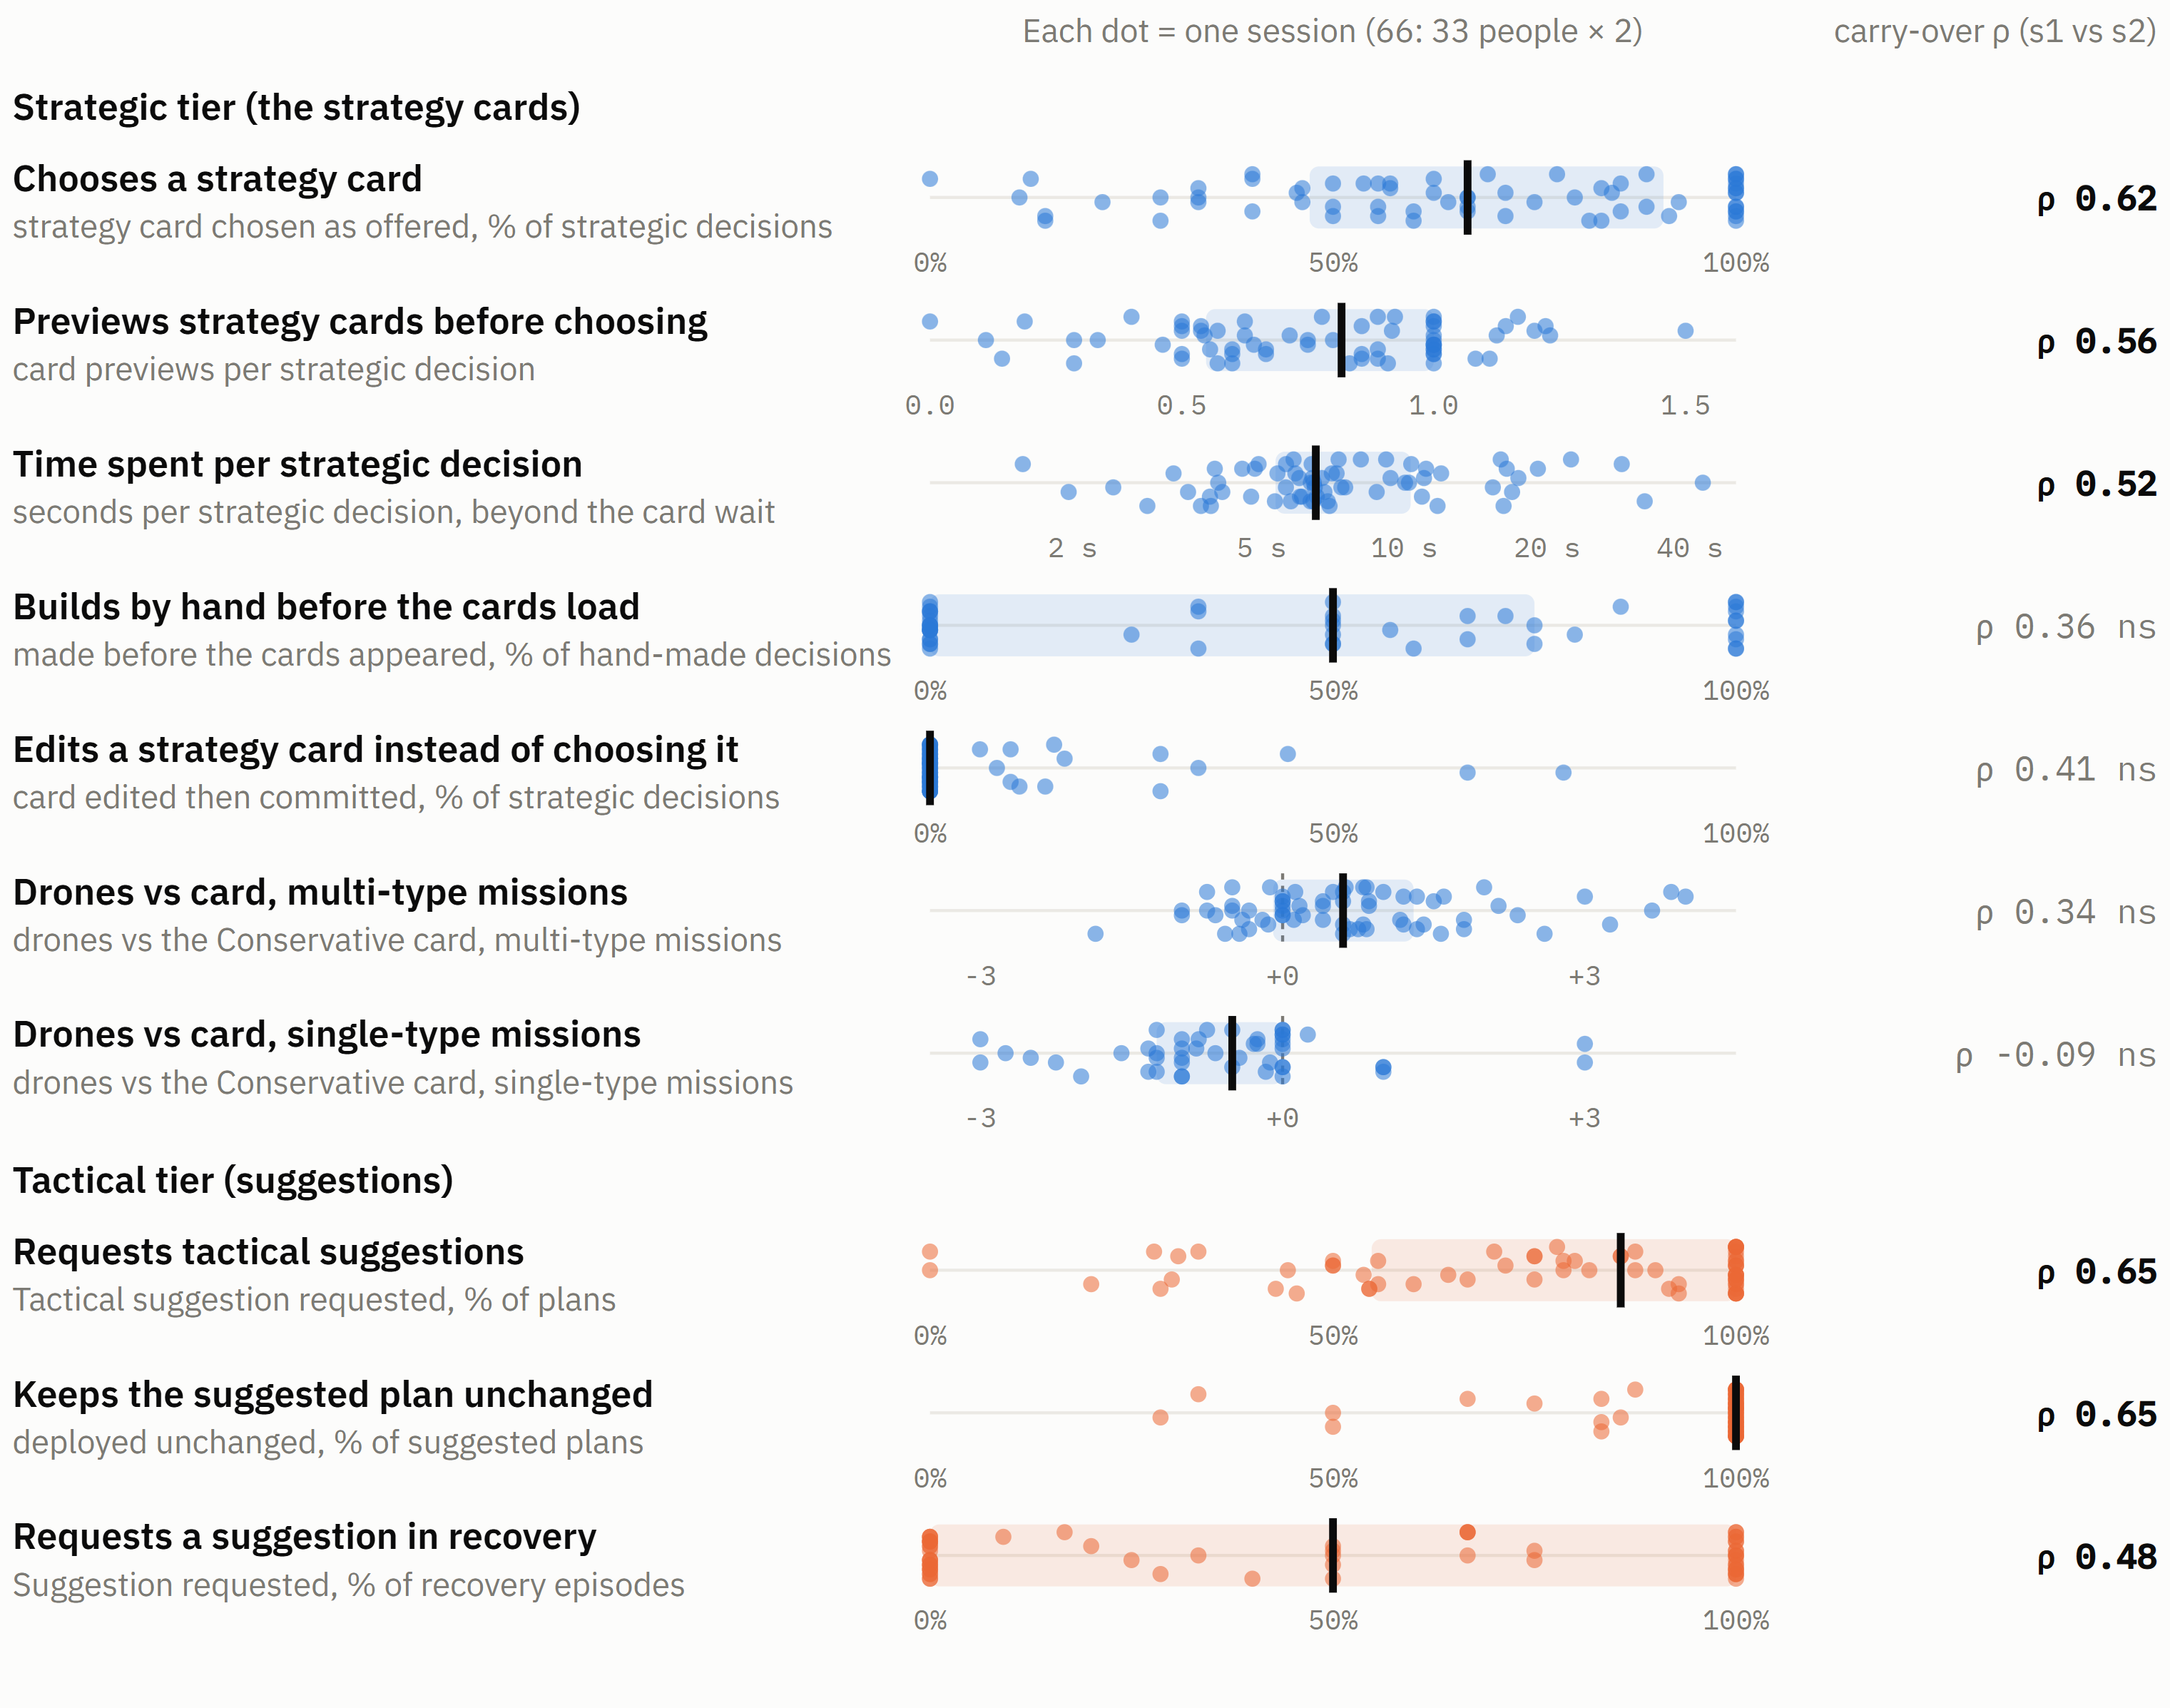
\includegraphics[width=\linewidth,height=0.50\textheight,keepaspectratio]{figs/results/f-personal-style__habits__main.png}
\caption{\textbf{The habits describing each user and how they vary.} These ten habits accurately describe a user and many carry over to that user's following scenario.}
\label{fig:res:personal-style:habits}
\end{figure}

% --- f-personal-style#fingerprint-ranks (pass 5: for the paper) ---

\phantomsection\label{sec:res:personal-style:fingerprint-ranks}
When asked to describe their approach, 15 of 33 named a consistent strategy of their own. In Figure~\ref{fig:res:personal-style:fingerprint-ranks:all}, each person's ten-habit profile from session 1 is compared with all 33 session-2 profiles, and the 33 are ranked from most to least alike (and the same the other way round, session 2 among the session 1s) by Euclidean distance over the 10 dimensions. If habits were not personal, a person's own other session would be equally likely to land anywhere in that ranking (dashed line). Instead it is the single closest match 12 times out of 66 (2 expected by chance) and in the closest three 27 times (6 expected), even though the second session is a different scenario ($p < .001$).

\begin{figure}[H]
\centering
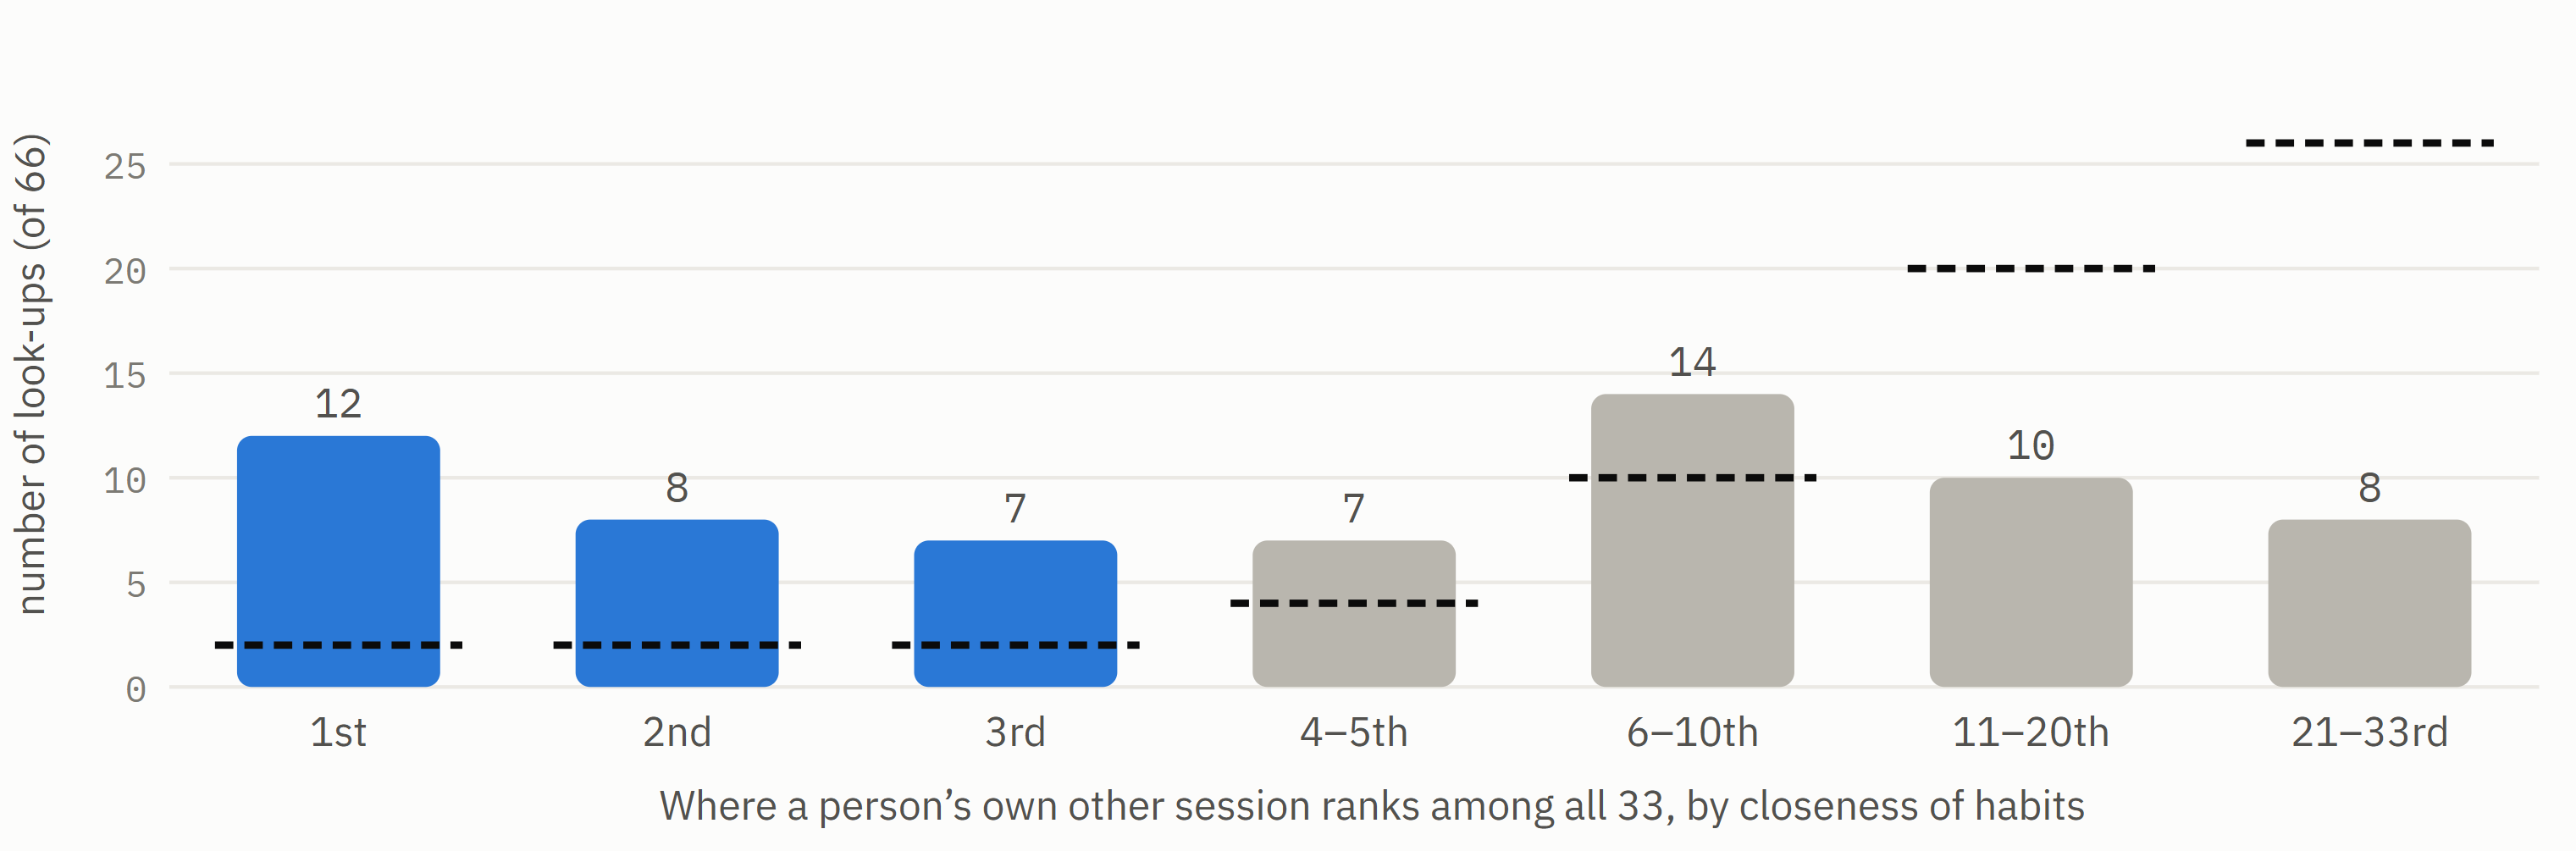
\includegraphics[width=\linewidth,height=0.50\textheight,keepaspectratio]{figs/results/f-personal-style__fingerprint-ranks__all.png}
\caption{\textbf{A person's own other session is usually among their closest matches.} Where each person's own session ranks among all 33 by ten-habit profile; dashed line: where it would fall if habits were not personal.}
\label{fig:res:personal-style:fingerprint-ranks}
\label{fig:res:personal-style:fingerprint-ranks:all}
\end{figure}

% --- f-personal-style#who-vs-what (pass 5: for the paper) ---

\phantomsection\label{sec:res:personal-style:who-vs-what}
When inspecting every instance of a user choosing or not choosing a strategy card, knowing \textit{who} is deciding predicts whether a card is chosen about six times better than knowing everything about the mission and when it arrived. We built three logistic models with access to different priors about the decision. Knowing only \textit{who} made the choice, the model classified the right one 75\% of the time (a coin: 50\%; knowing only the mission: 63\%). A person's session-1 rate on its own still does it 71\% of the time for their session-2 decisions. Figure~\ref{fig:res:personal-style:who-vs-what:r2} shows this as a set of $R^2$ values.

\begin{figure}[H]
\centering
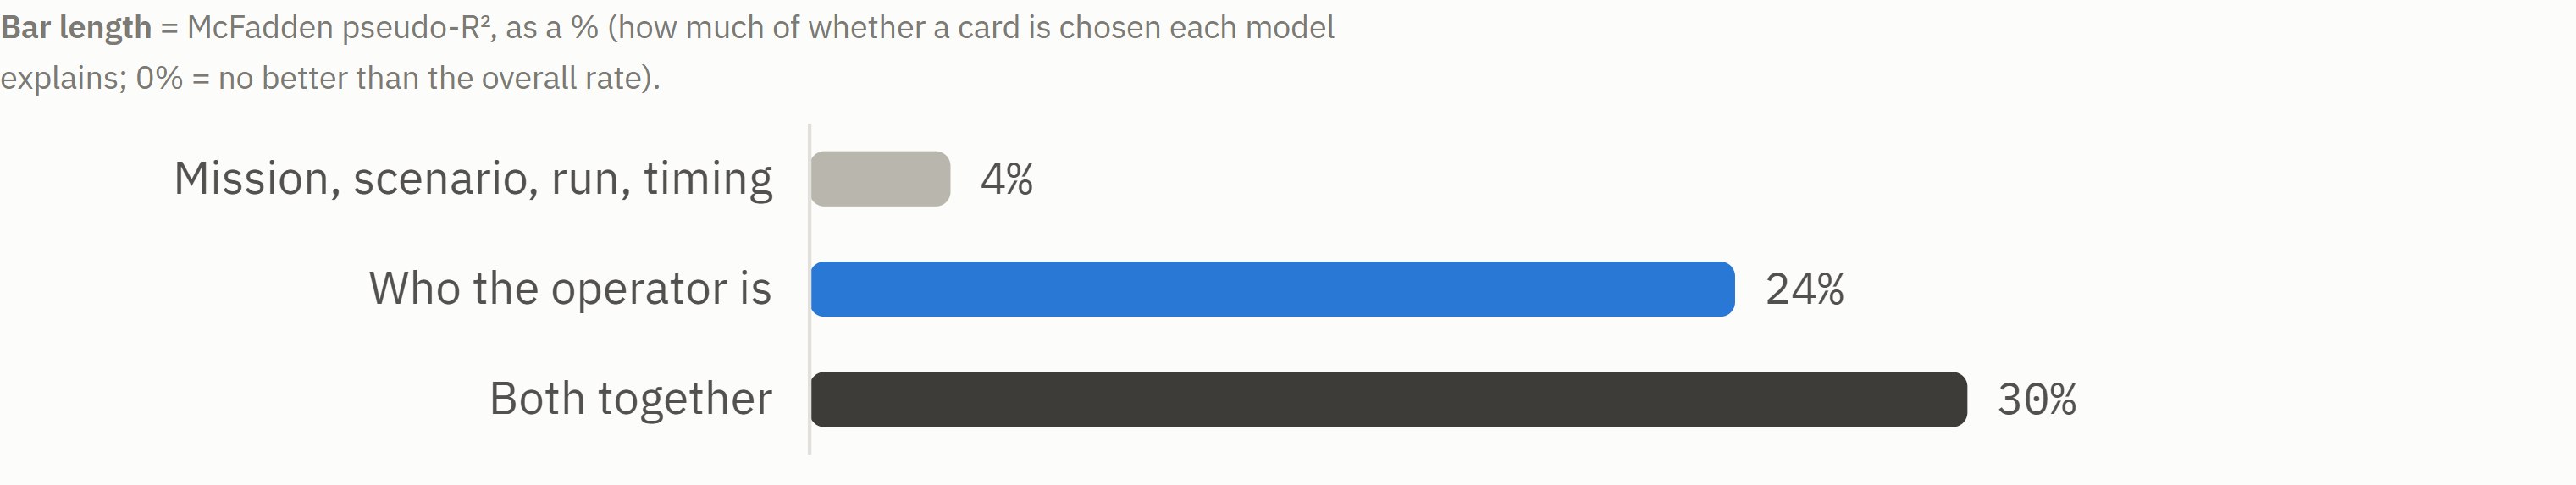
\includegraphics[width=\linewidth,height=0.50\textheight,keepaspectratio]{figs/results/f-personal-style__who-vs-what__r2.png}
\caption{\textbf{Who decides explains far more of strategy card choice than what is being decided.} McFadden pseudo-$R^2$ of models predicting whether a strategy card is chosen from the mission and its timing, from the person, and from both.}
\label{fig:res:personal-style:who-vs-what}
\label{fig:res:personal-style:who-vs-what:r2}
\end{figure}

People often described their use of the assistants as part of who they are, and in a highly varied sense: `naturally conservative' (P32), `I'm more conservative' (P26), `I always let the agent do it first' (P13). At the extremes, P14 used the assistants `for almost every allocation' and P16 `manually overrode most of the time'. P32 calls themself `naturally conservative' and also says their use was `very much about workload', so a person's style and the situation are both in play.

% --- f-personal-style#axis-scatter (pass 5: for the paper) ---

\phantomsection\label{sec:res:personal-style:axis-scatter}
Participants' strategic and tactical reliance correlated only slightly. Figure~\ref{fig:res:personal-style:axis-scatter:between} shows each participant's proportional use of each assistant. The correlation between use of the two assistants is only $\rho = 0.37$.

\begin{figure}[H]
\centering
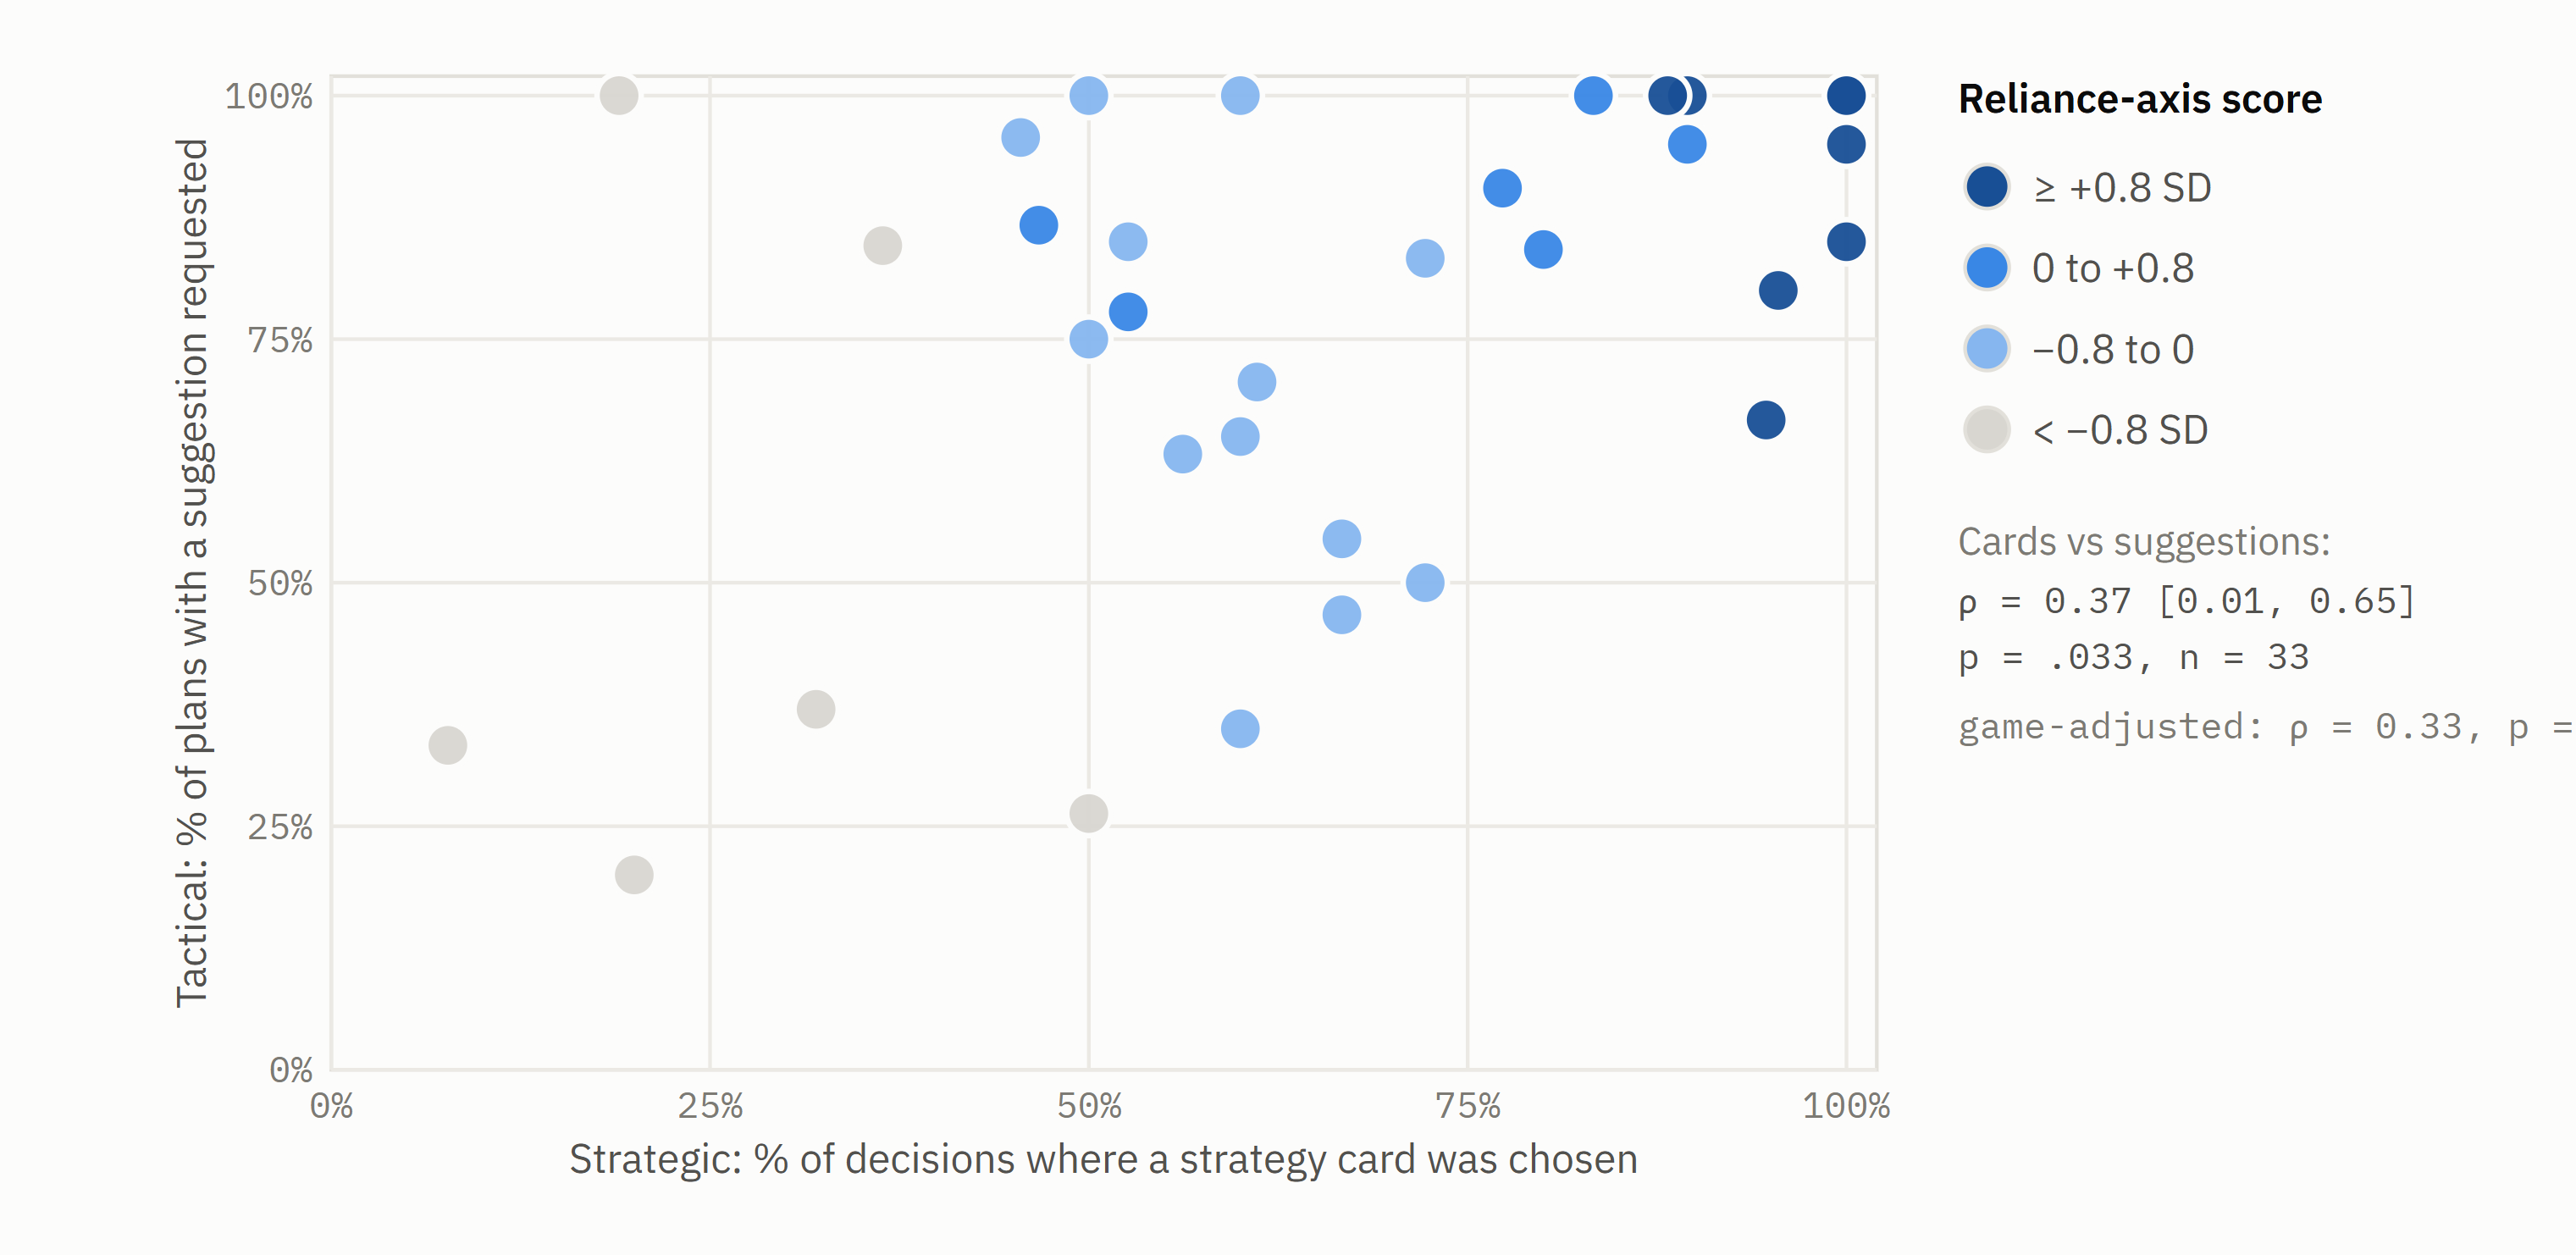
\includegraphics[width=\linewidth,height=0.50\textheight,keepaspectratio]{figs/results/f-personal-style__axis-scatter__between.png}
\caption{\textbf{Use of one assistant says little about use of the other.} Each dot is a person: the share of their strategic decisions where a strategy card was chosen, against the share of their tactical plans where a suggestion was requested.}
\label{fig:res:personal-style:axis-scatter}
\label{fig:res:personal-style:axis-scatter:between}
\end{figure}

% --- f-personal-style#not-types (pass 5: numbers only) ---

\phantomsection\label{sec:res:personal-style:not-types}
The styles are individual rather than types. Placed on their two largest habit dimensions, the 33 operators form one continuous cloud that looks like a set of simulated operators with no types by construction (Figure~\ref{fig:res:personal-style:not-types:map}). However many groups we ask for (two, three or four), the real people separate no better than the simulations do (silhouette .17--.20 against .19--.20), and groups found in one session barely come back in the other (adjusted Rand index .08--.09, against .13 for a smooth cloud in which people keep their place).

\begin{figure}[H]
\centering
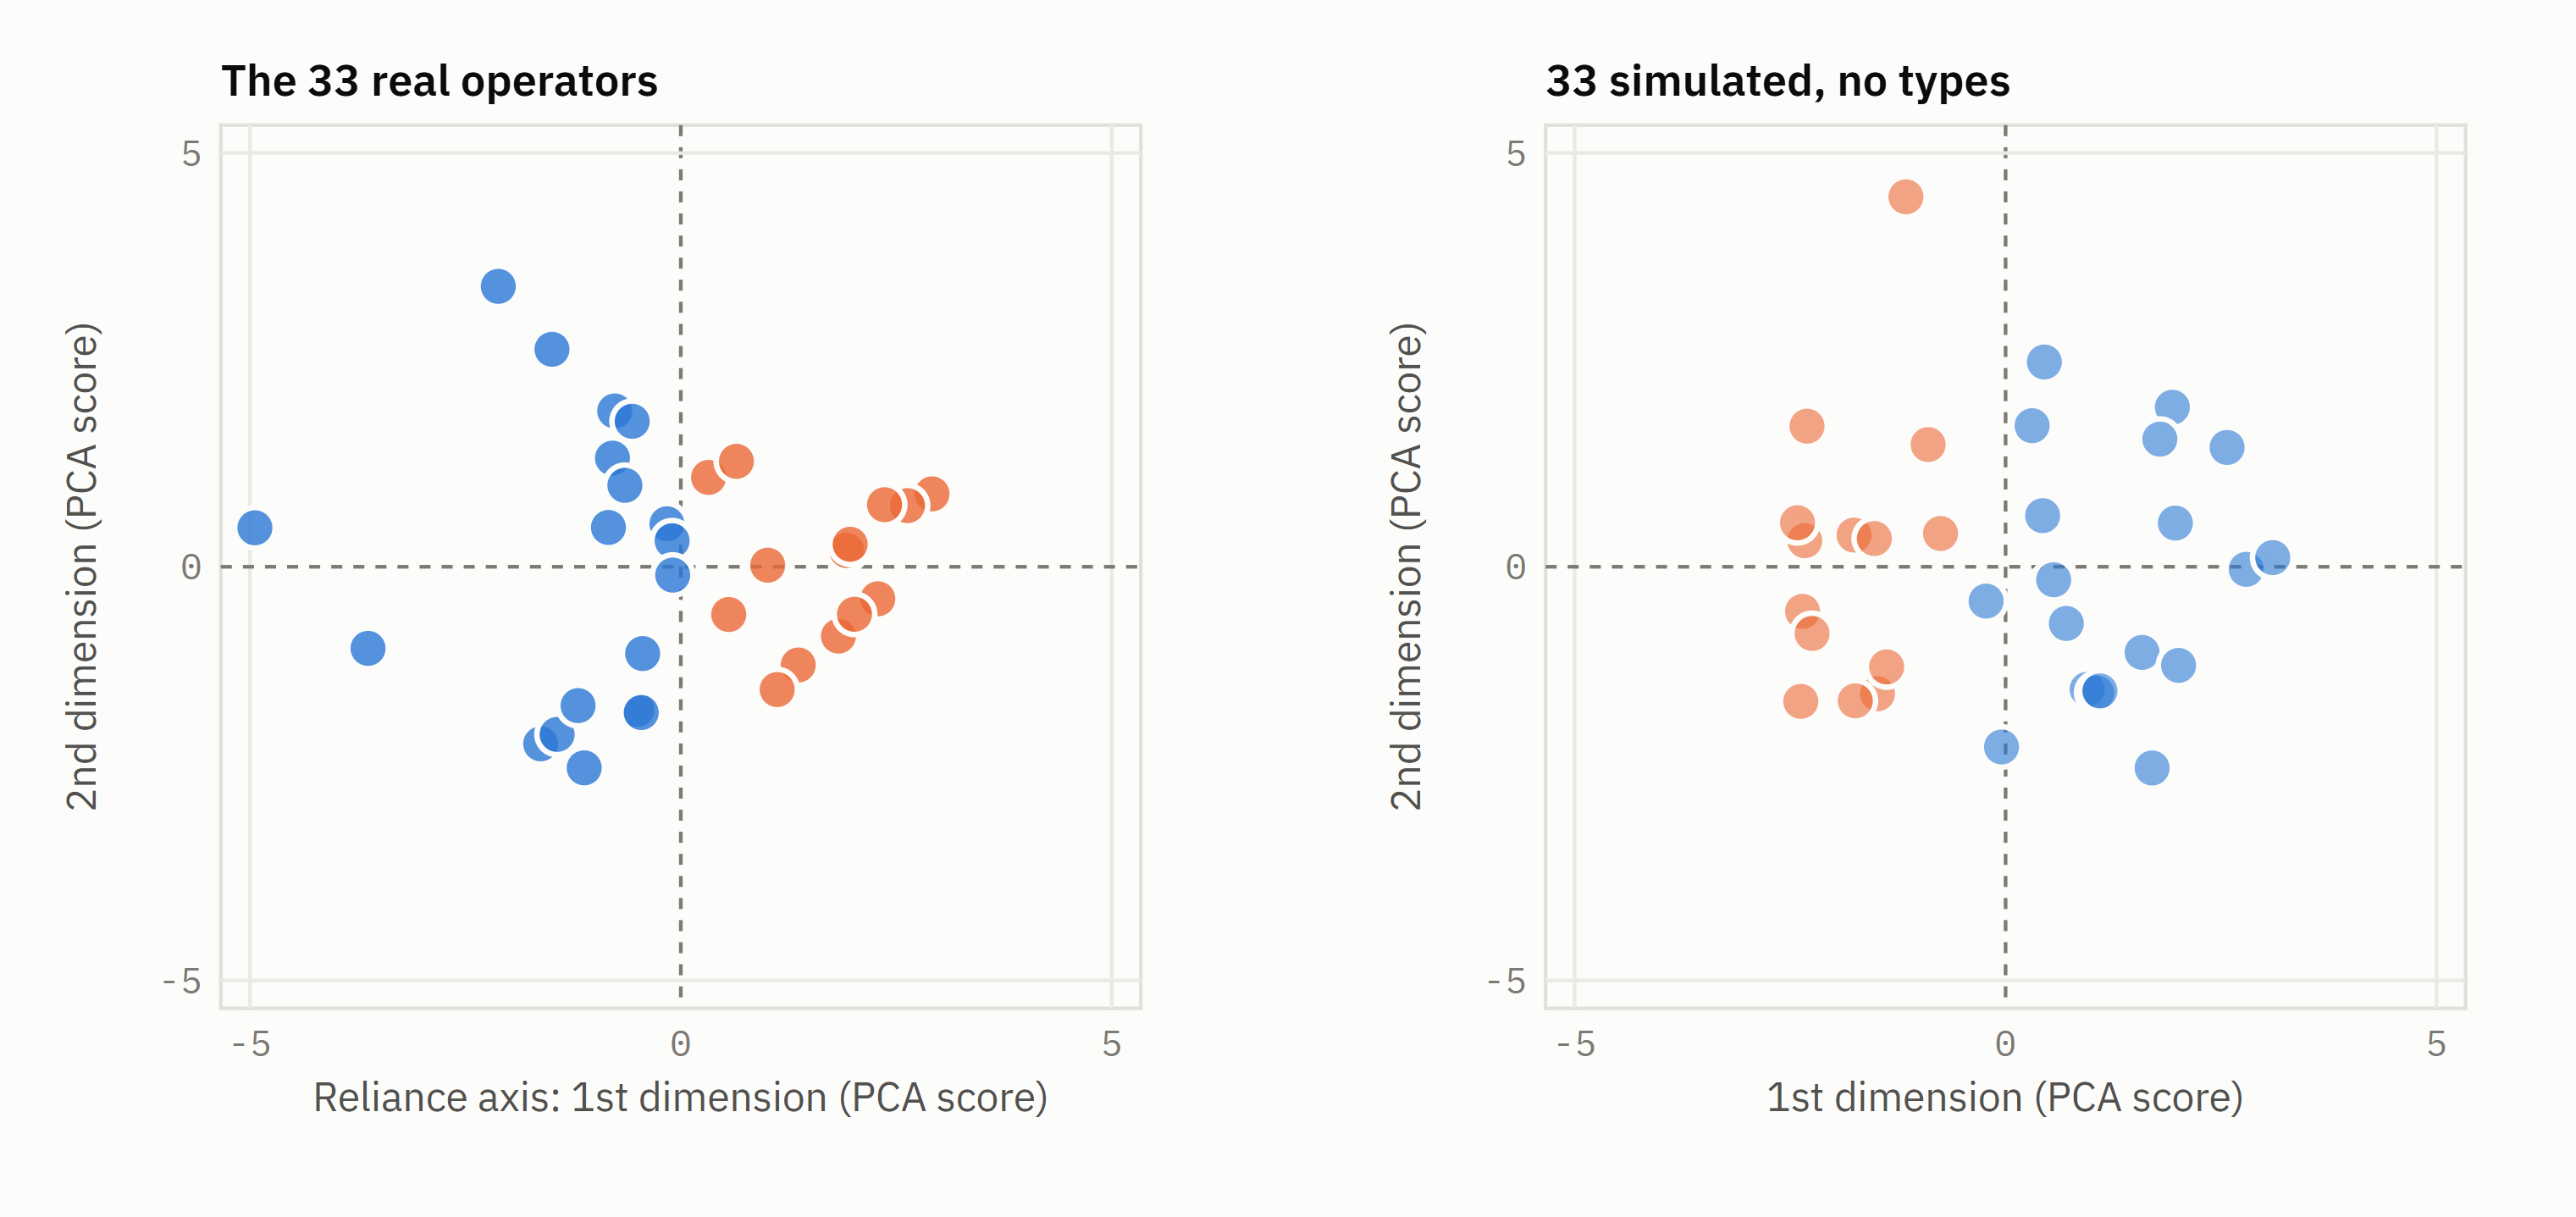
\includegraphics[width=\linewidth,height=0.50\textheight,keepaspectratio]{figs/results/f-personal-style__not-types__map.png}
\caption{\textbf{No types: the operators form one continuous cloud.} Each person placed on the first two principal components of the ten habits.}
\label{fig:res:personal-style:not-types}
\label{fig:res:personal-style:not-types:map}
\end{figure}

% --- f-personal-style#not-disposition (pass 5: for the paper) ---

\phantomsection\label{sec:res:personal-style:not-disposition}
Nothing measured before the study predicts a person's style. Of 40 tests of attitude to AI (AIAS-4), verification propensity, views on human authority and prior experience against five behaviours, three reach $p < .05$ and none survives Holm correction; chance alone gives two such hits on average, and three or more in a third of shuffles (Figure~\ref{fig:res:personal-style:not-disposition}). This is an absence of evidence rather than evidence of no link: with 33 people only correlations of $|\rho| \geq .48$ could be detected, and the sample is uniformly positive about AI (AIAS-4 mean 8.0 of 10). In their own words, people's general views on AI did not line up with what they did, and most explained their use by time pressure and job size rather than by a view about AI.

\begin{figure}[H]
\centering
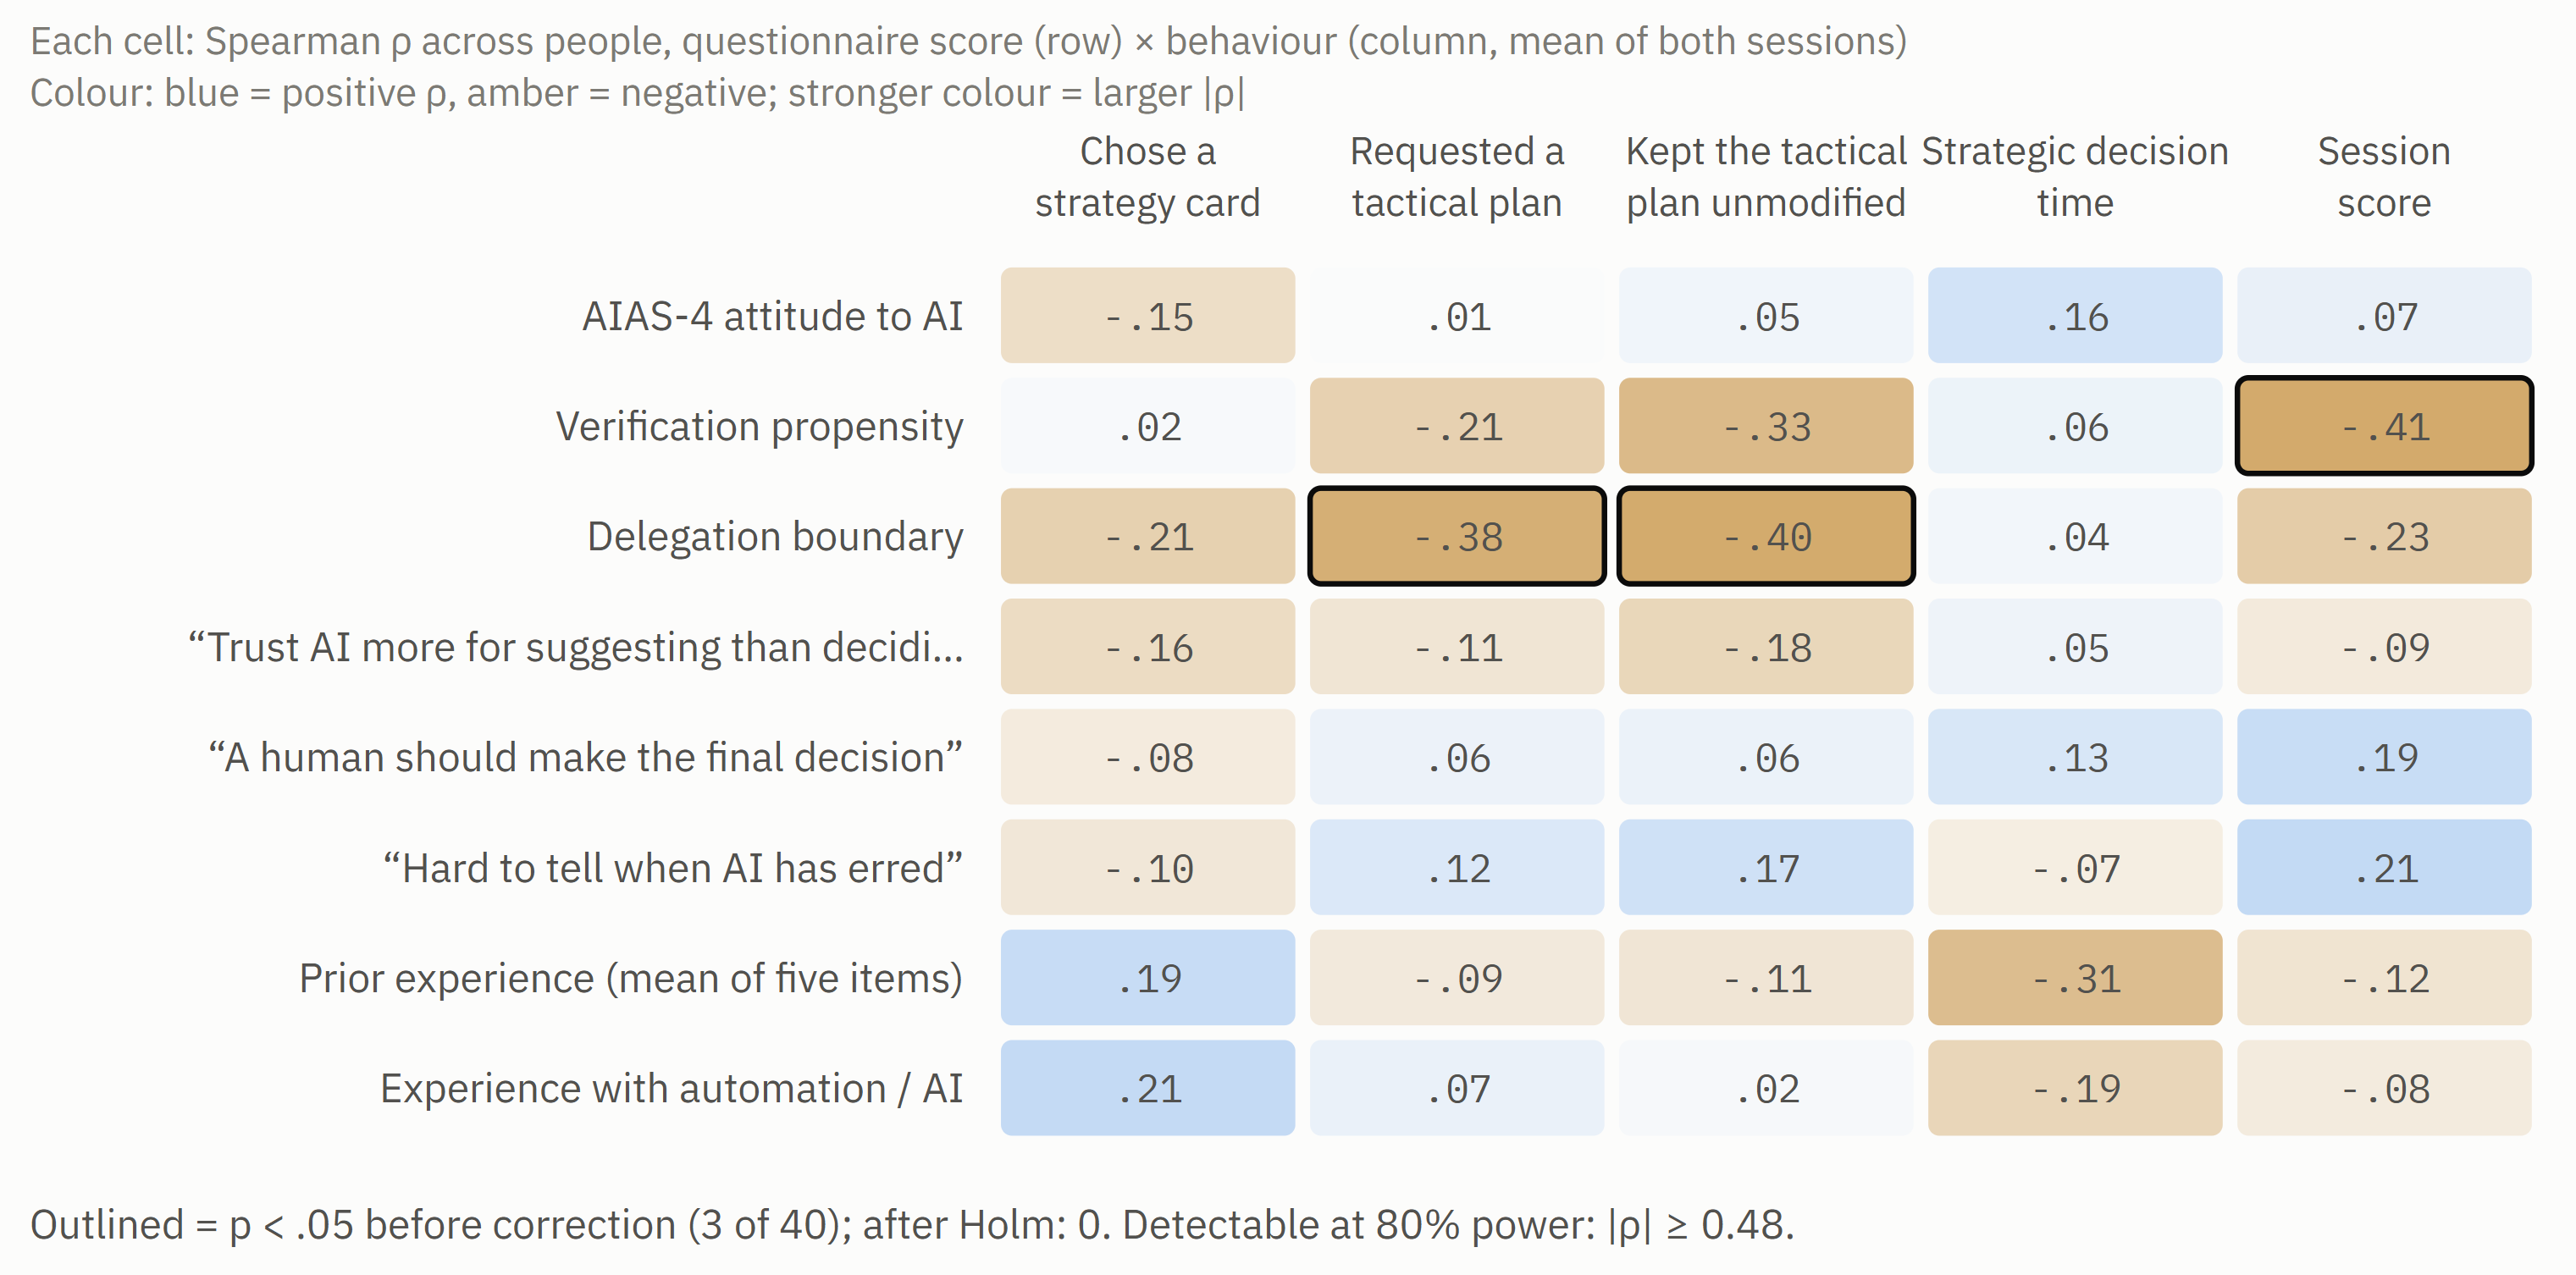
\includegraphics[width=\linewidth,height=0.50\textheight,keepaspectratio]{figs/results/f-personal-style__not-disposition__main.png}
\caption{\textbf{Nothing measured beforehand predicts style.} Correlations between the pre-study scales and five behaviours; none survives correction for the 40 tests.}
\label{fig:res:personal-style:not-disposition}
\end{figure}

\begin{options}
\optshead{Options for this finding}

\optsec{The habits we grade them on} {\footnotesize [pass 5: numbers only]}

\noindent Key numbers:\begin{itemize}[leftmargin=1.2em,itemsep=0pt]\footnotesize
\item Strategy card chosen as offered: median 67\% of a session's strategic decisions (middle half 47--91\%, range 0--100\%)
\item suggestion requested: median 86\% of tactical plans (55--100\%); suggested plan kept unchanged: median 100\% (middle half 100--100\%)
\item Decision time beyond the card wait: median 6.5 s (5.4--10.3 s, range 1.6--43 s)
\item Card edited before committing: median 0\% (most sessions never); going manual before the cards appear: median 50\% of hand-made decisions (0--75\%)
\item Drones vs the Conservative card: single-type $-$0.5 ($-$1.25 to 0); multi-type +0.6 ($-$0.1 to +1.3)
\end{itemize}

\optsec{Where each person's own session ranks} {\footnotesize [pass 5: for the paper]}

\par\noindent \begin{minipage}[t]{0.49\linewidth}\centering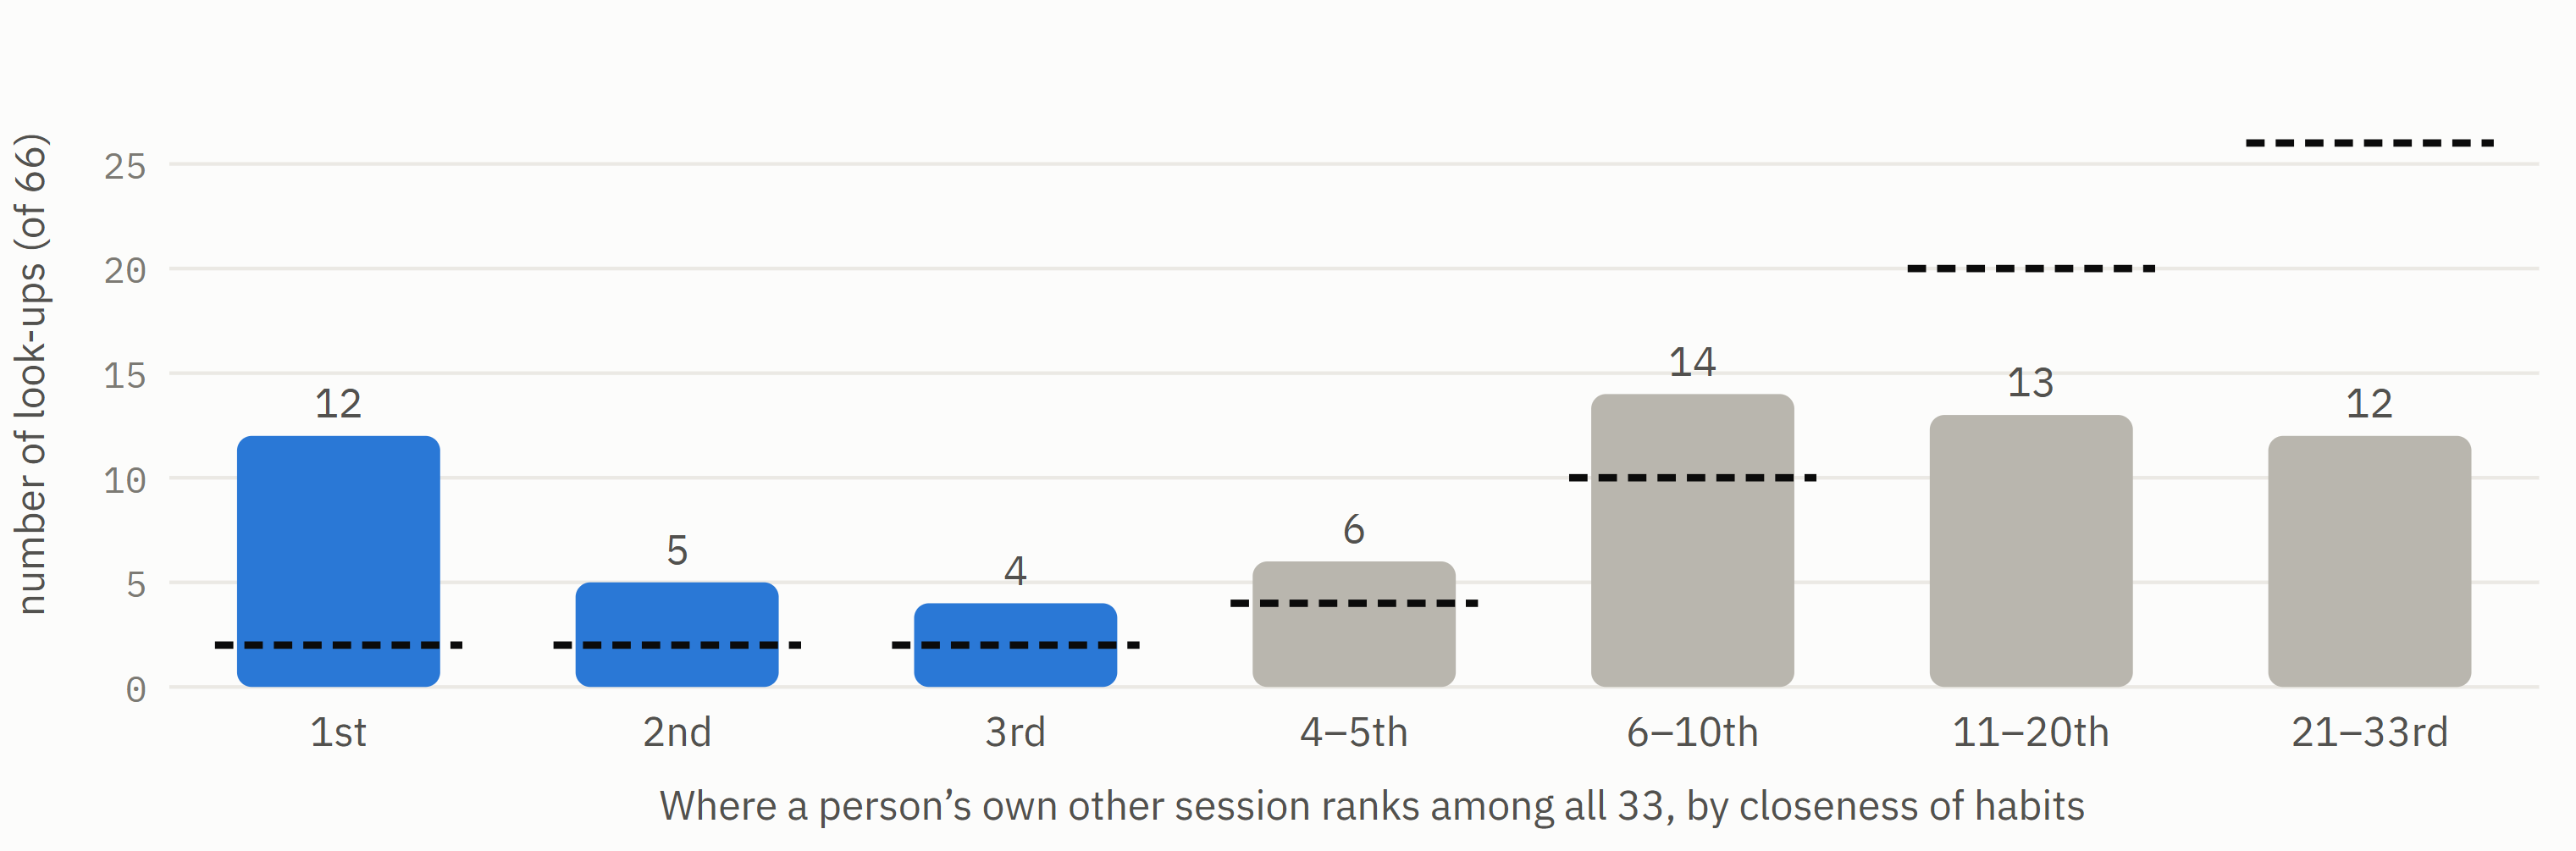
\includegraphics[width=\linewidth,height=0.24\textheight,keepaspectratio]{figs/results/f-personal-style__fingerprint-ranks__noaxis.png}\par{\scriptsize Other view: With the reliance axis removed.}\end{minipage}

\noindent Key numbers:\begin{itemize}[leftmargin=1.2em,itemsep=0pt]\footnotesize
\item Own session ranked 1st: 12 of 66 look-ups vs 2 expected; in the closest three: 27 vs 6 (41\% vs 9\%); permutation p < .001
\item Average rank of own session 8.2 of 33 (chance 17.0); with the reliance axis removed 10.1 (p < .001)
\item Profile correlation with own other session: median r = .48; with other people's: median r = $-$.01; own closer for 29 of 33
\end{itemize}

\optsec{Who decides matters more than what is being decided} {\footnotesize [pass 5: for the paper]}

\par\noindent \begin{minipage}[t]{0.49\linewidth}\centering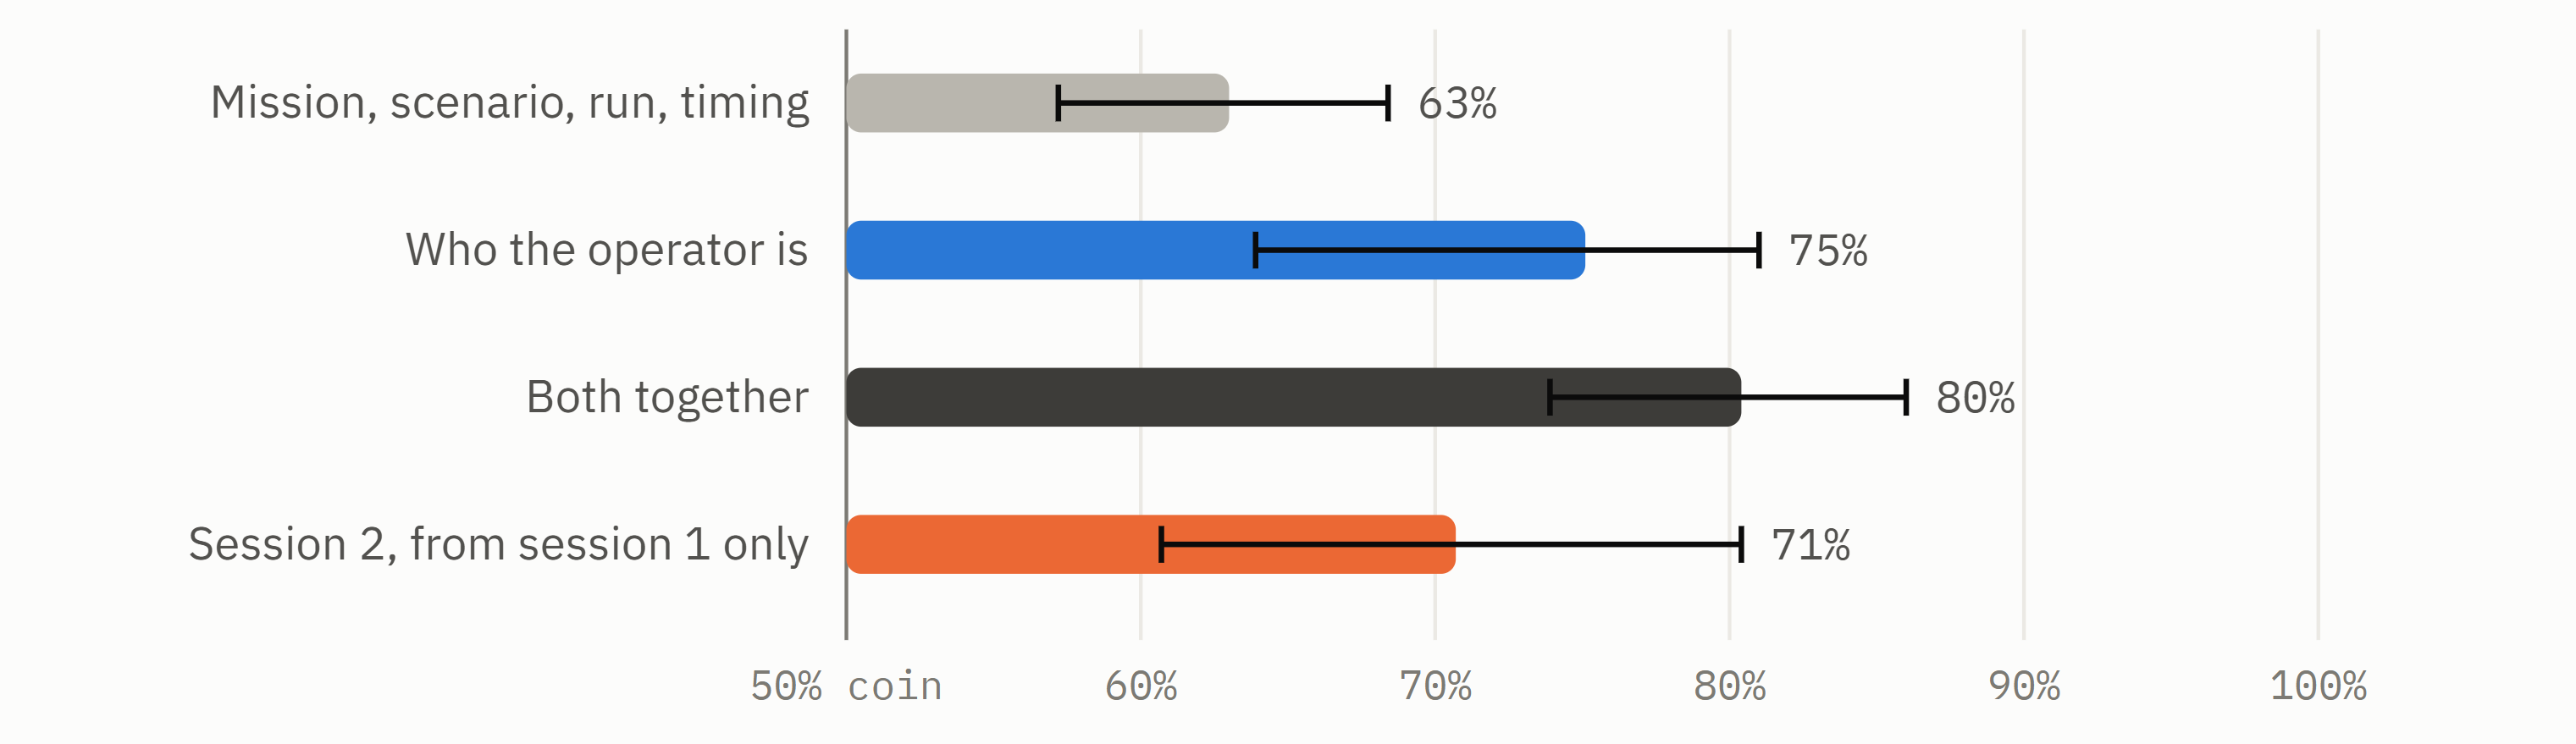
\includegraphics[width=\linewidth,height=0.24\textheight,keepaspectratio]{figs/results/f-personal-style__who-vs-what__auc.png}\par{\scriptsize Other view: The same comparison as a ranking test (AUC); whiskers are 95\% intervals (people resampled).}\end{minipage}

\noindent Key numbers:\begin{itemize}[leftmargin=1.2em,itemsep=0pt]\footnotesize
\item Pseudo-R$^2$: mission + timing 4\%; person 24\%; both 30\%
\item Strategy card choice per person 8\%--100\%, median 61\%; 6 people $\geq$ 90\%, 3 people $\leq$ 25\%
\item Telling a taken from a not-taken decision (AUC): mission and timing 63\% [57\%, 68\%]; the person, from their other decisions, 75\% [64\%, 81\%]; both 80\% [74\%, 86\%]; session-2 decisions from the session-1 rate alone 71\% [61\%, 80\%] (321 decisions).
\item Right-or-wrong guessing: always 'card' 66\%; mission 65\%; person 70\%; both 77\%.
\item Person-only pseudo-R$^2$ with the person labels shuffled: 4\% on average (95th percentile 6\%), against 24\% observed.
\end{itemize}

\optsec{How far each habit holds from one session to the next} {\footnotesize [pass 5: for the paper; not used in the prose above]}

\noindent\regtext{One line per habit: how strongly a person's place on that habit in session 1 predicts their place in session 2 ($\rho$; 0 = no carry-over, 1 = same order of people). Six of the ten carry over clearly and survive correction for testing ten (coloured). Editing cards, going manual before the cards load and topping up drones on multi-type missions carry over weakly, and topping up drones on single-type missions does not carry over at all ($\rho$ $-$.09). ``Keeps the suggested plan'' is high partly because 24 of 33 people kept every suggested plan in both sessions.}

\par\noindent \begin{minipage}[t]{0.49\linewidth}\centering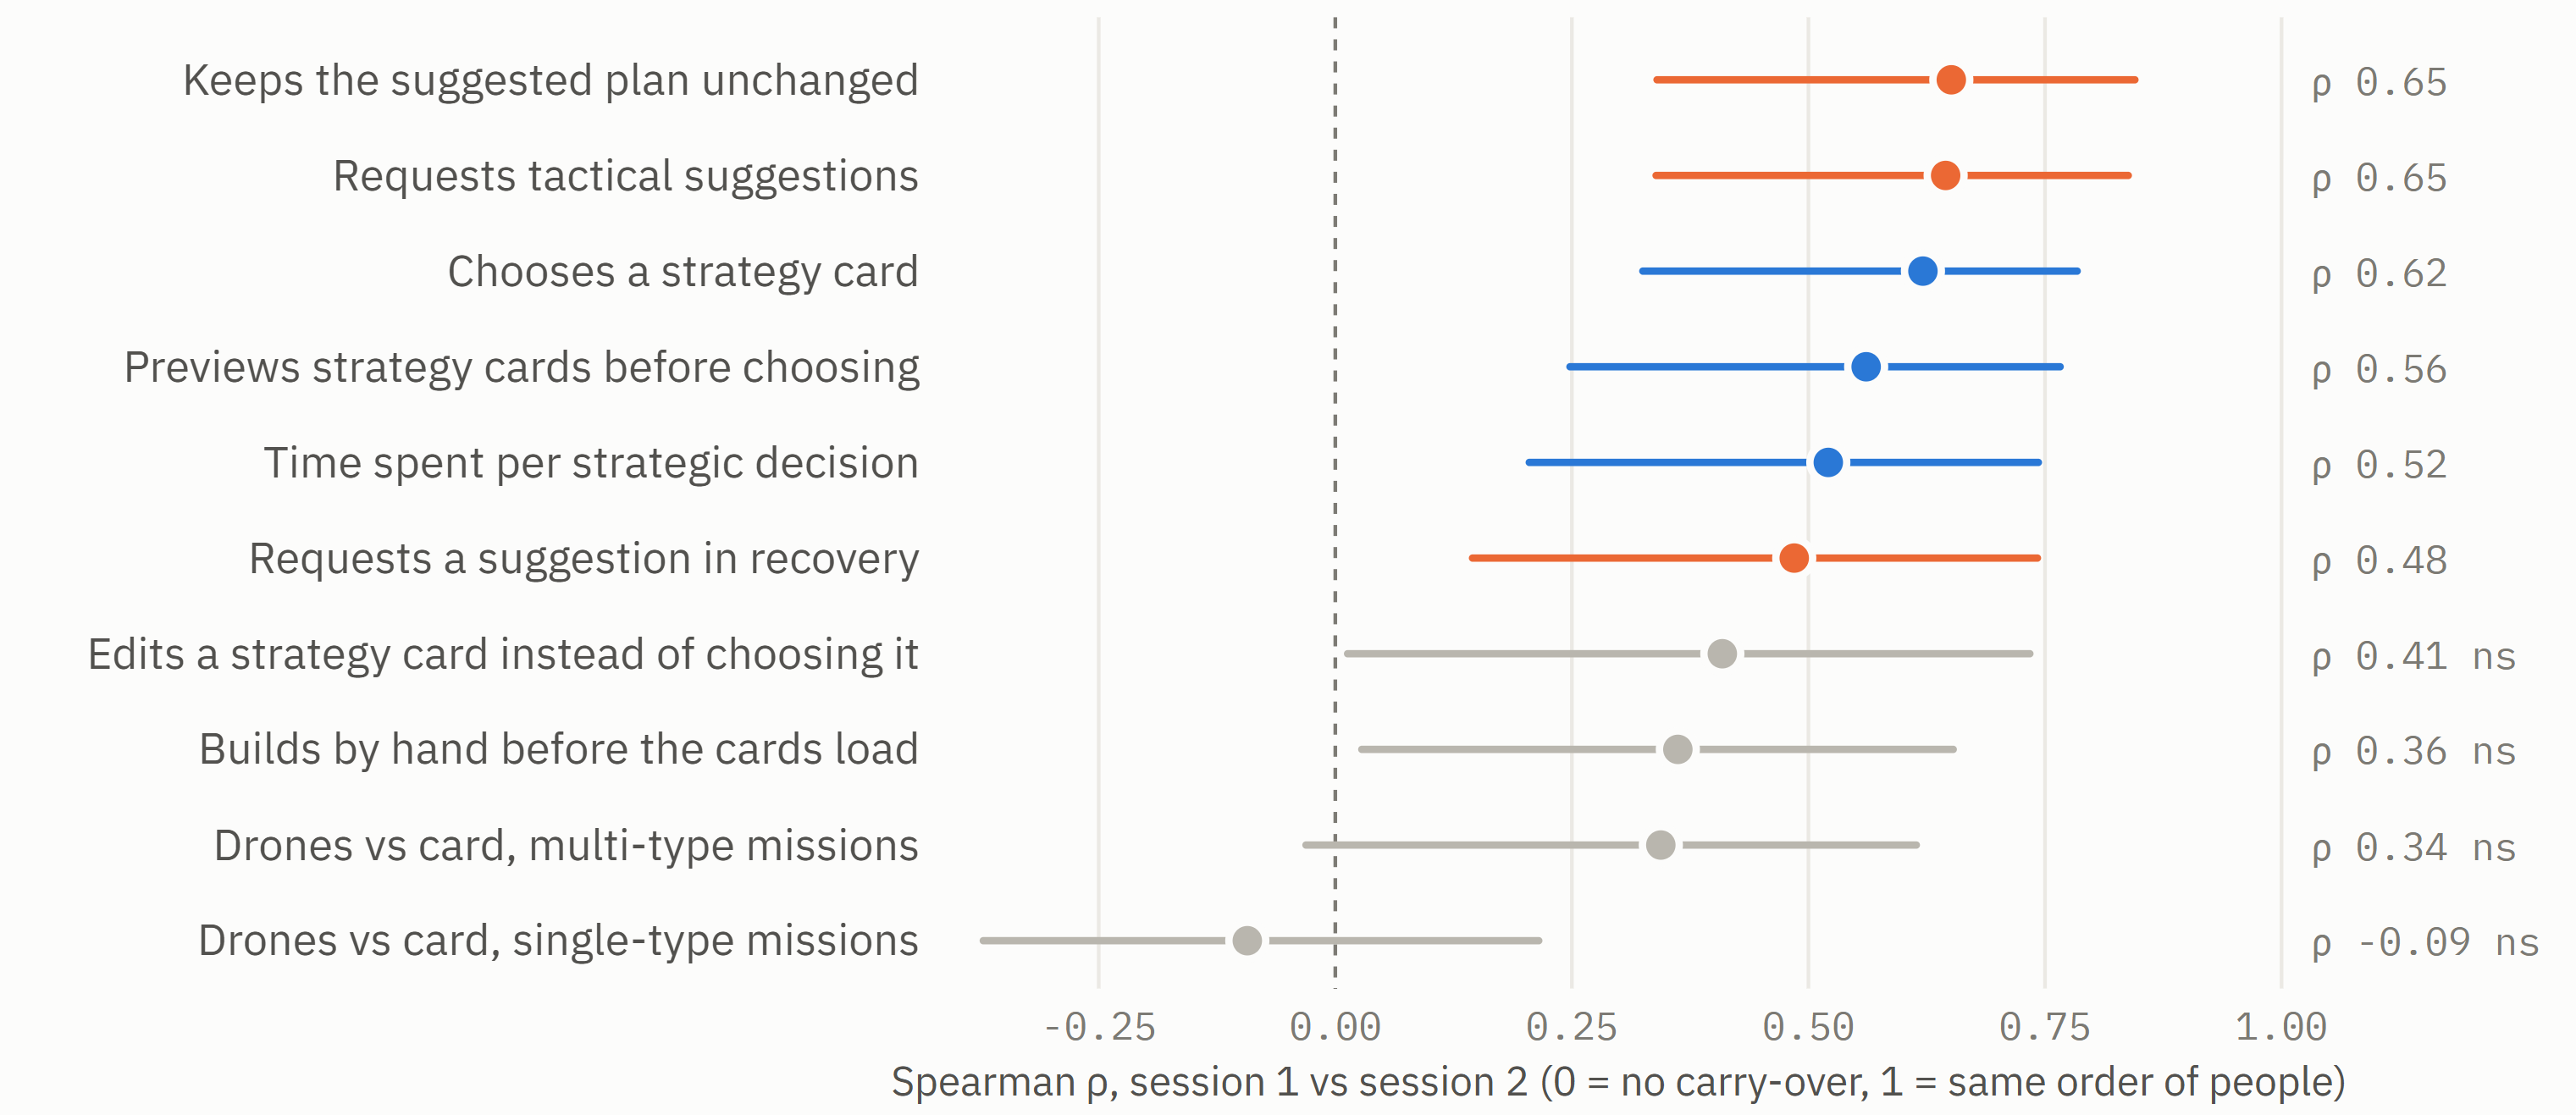
\includegraphics[width=\linewidth,height=0.24\textheight,keepaspectratio]{figs/results/f-personal-style__retest-summary__main.png}\par{\scriptsize main}\end{minipage}

\optsec{Strategic and tactical reliance go together only loosely between people} {\footnotesize [pass 5: for the paper]}

\par\noindent \begin{minipage}[t]{0.49\linewidth}\centering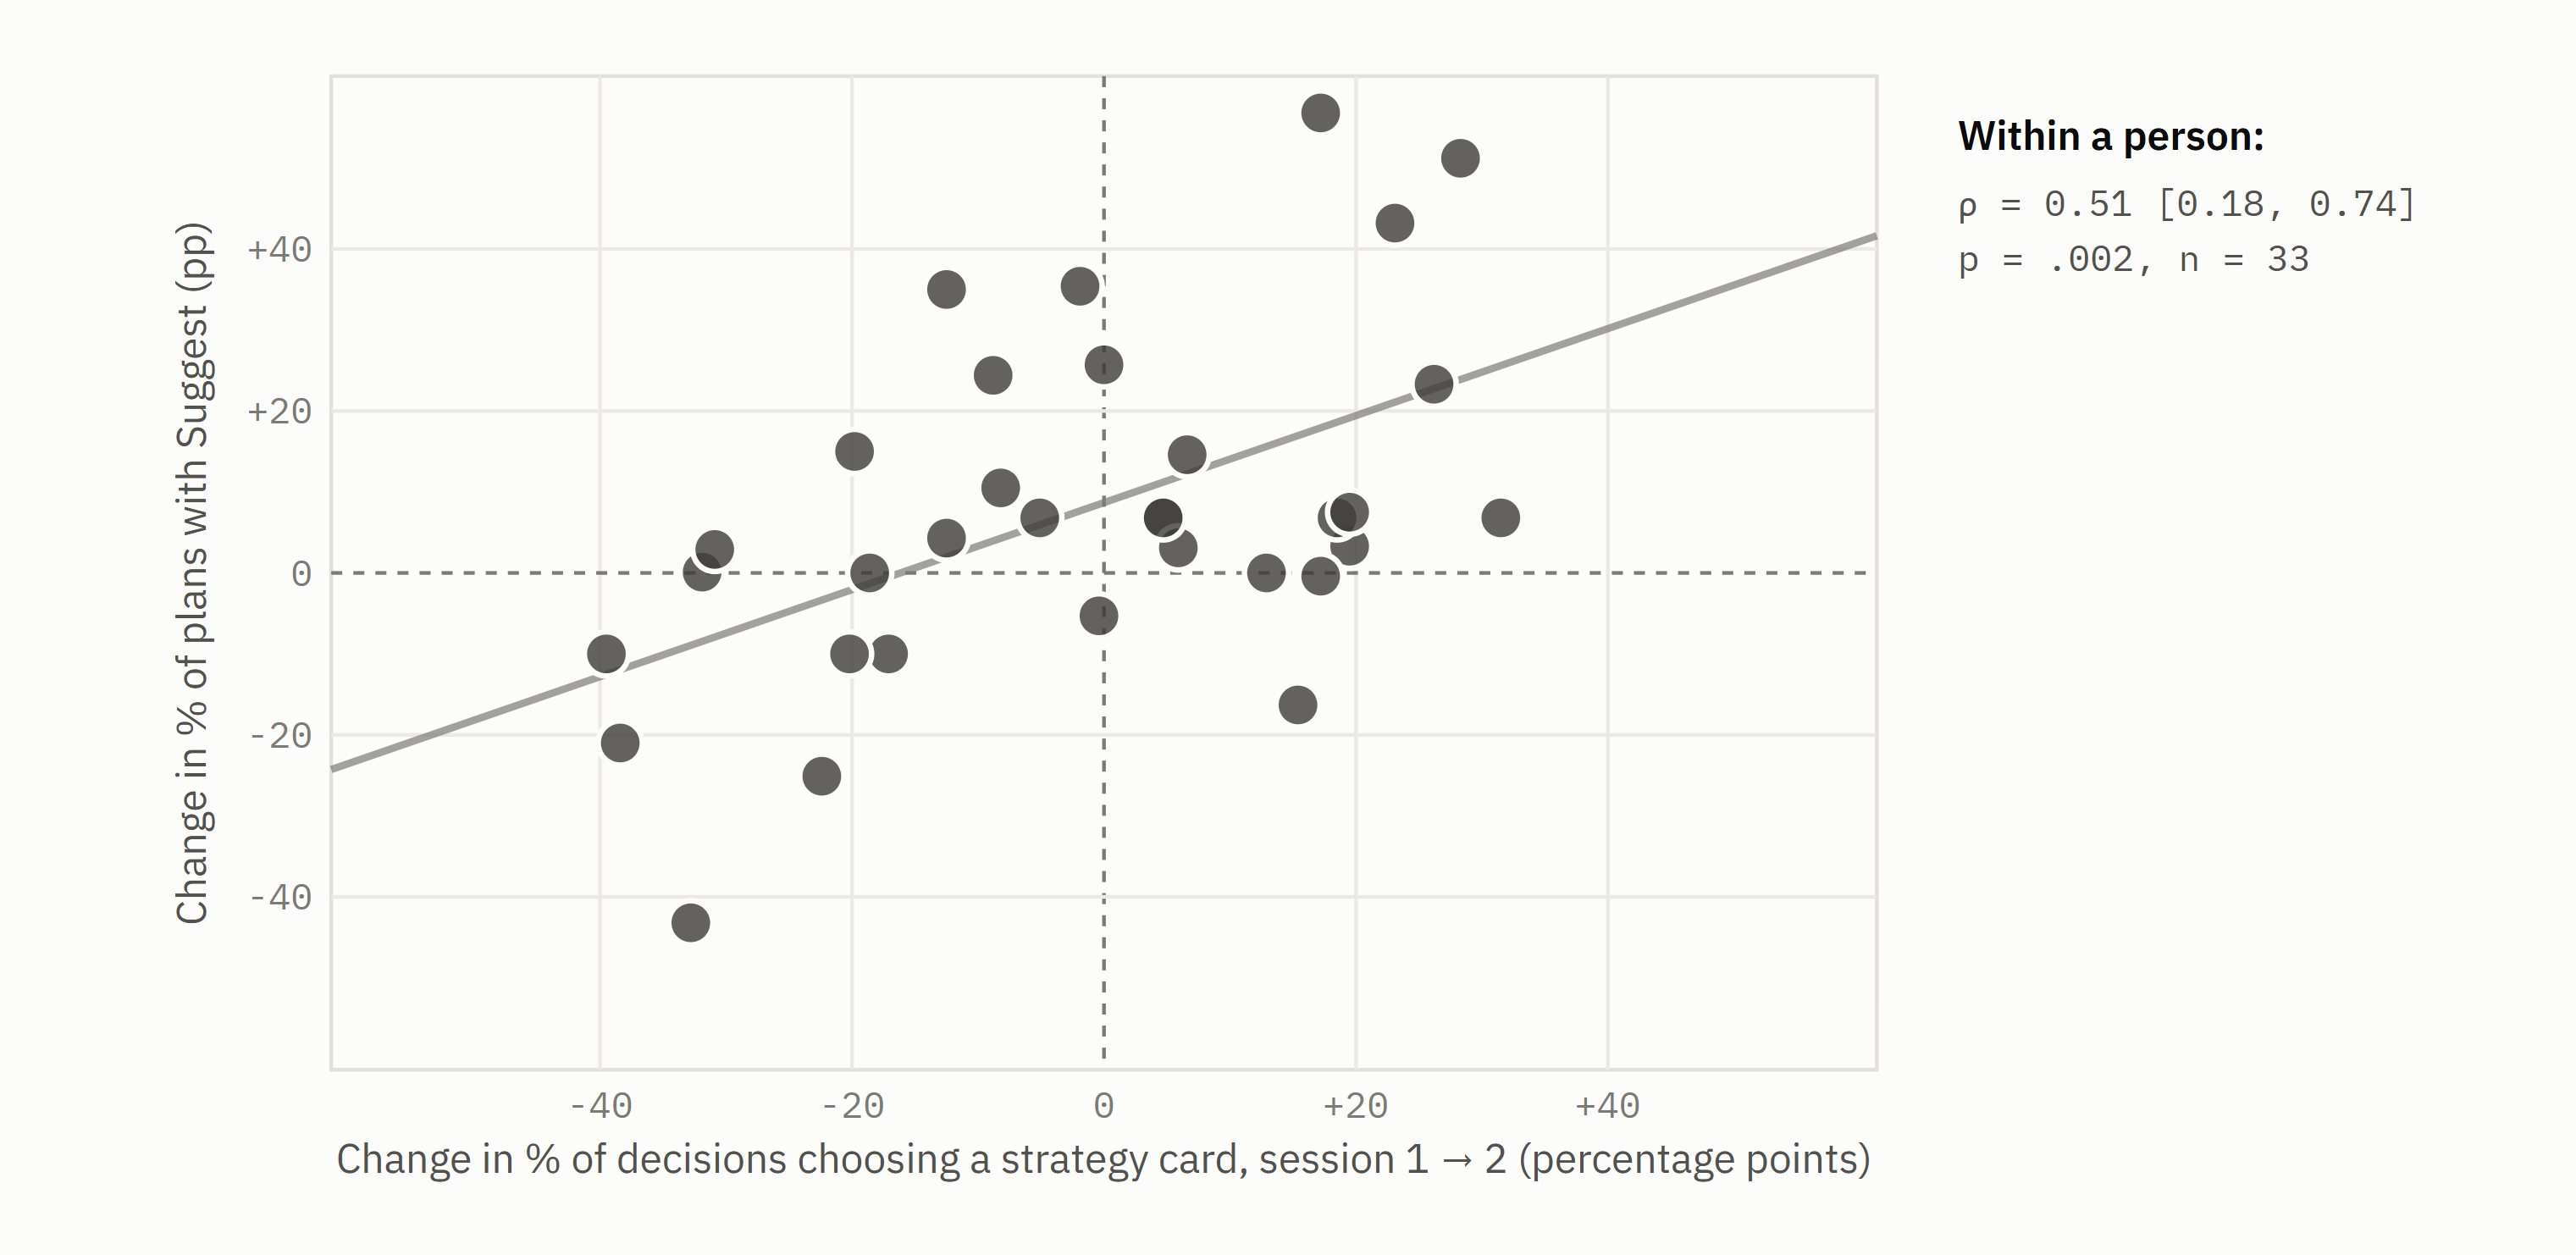
\includegraphics[width=\linewidth,height=0.24\textheight,keepaspectratio]{figs/results/f-personal-style__axis-scatter__within.png}\par{\scriptsize Other view: Within a person: change from session 1 to session 2.}\end{minipage}

\noindent Key numbers:\begin{itemize}[leftmargin=1.2em,itemsep=0pt]\footnotesize
\item Between people, strategy card choice vs tactical suggestion use: $\rho$ = .37 [.01, .65], p = .033 (raw); $\rho$ = .33 [$-$.03, .62], p = .058 (game-adjusted)
\item Within a person, change in strategy card choice vs change in tactical suggestion use, session 1 $\rightarrow$ 2: $\rho$ = .51 [.18, .74], p = .002
\item Strategy card choice vs Suggest in recovery: $\rho$ = .42, p = .014; vs keeping the suggested plan unchanged: $\rho$ = .20, p = .26
\item Card taking and previewing: $\rho$ = .79 (largely mechanical: choosing a card means clicking it)
\end{itemize}

\optsec{Individual, not types} {\footnotesize [pass 5: numbers only]}

\par\noindent \begin{minipage}[t]{0.49\linewidth}\centering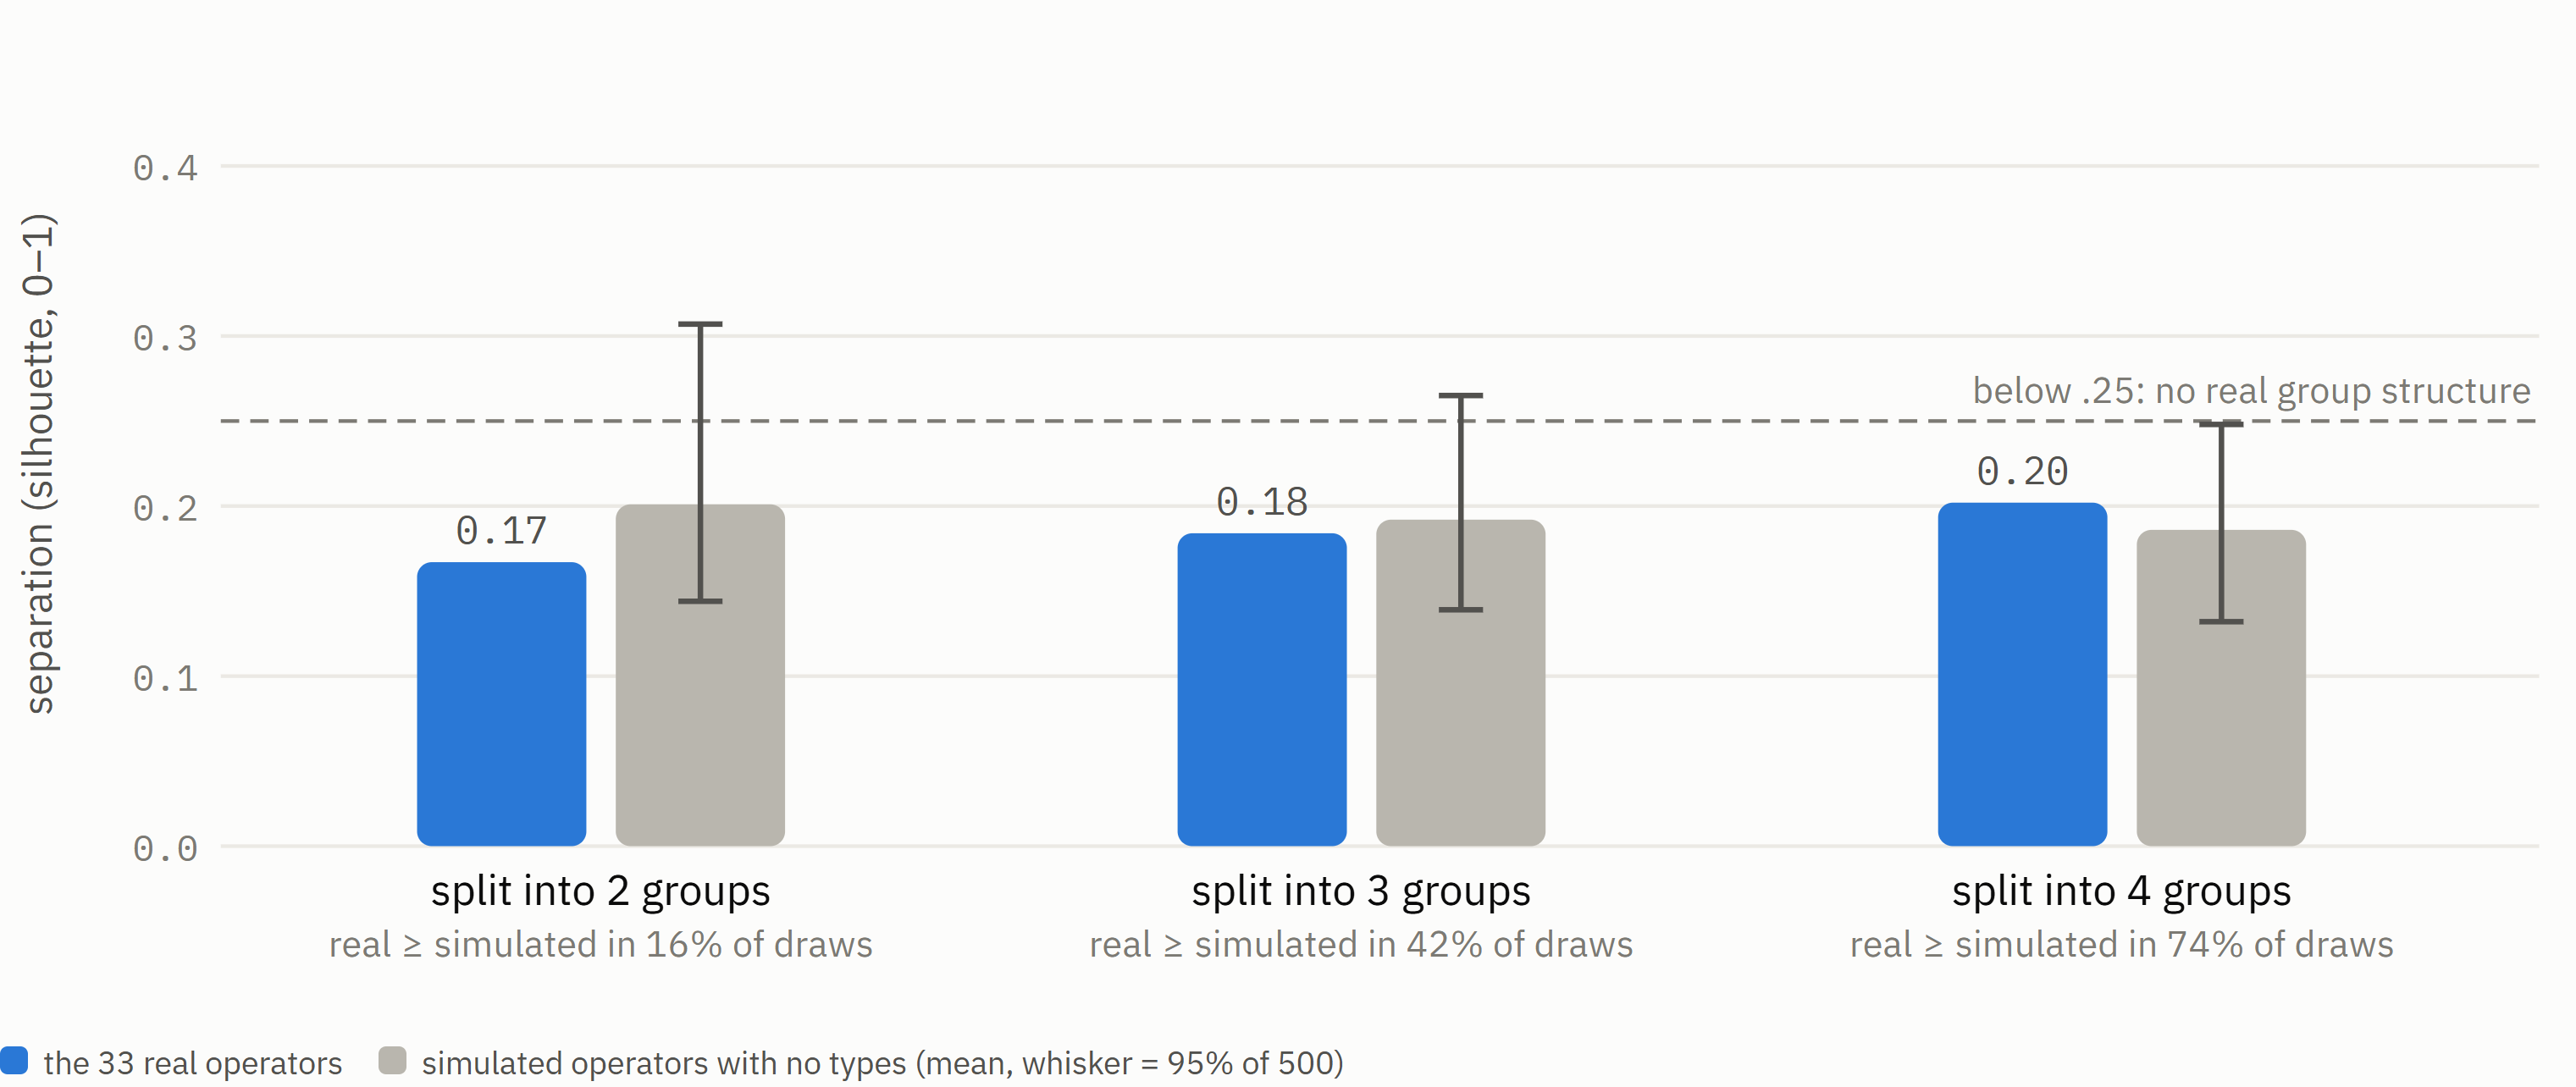
\includegraphics[width=\linewidth,height=0.24\textheight,keepaspectratio]{figs/results/f-personal-style__not-types__separate.png}\par{\scriptsize Other view: Cluster separation (silhouette) against no-types simulations.}\end{minipage}\hfill
\begin{minipage}[t]{0.49\linewidth}\centering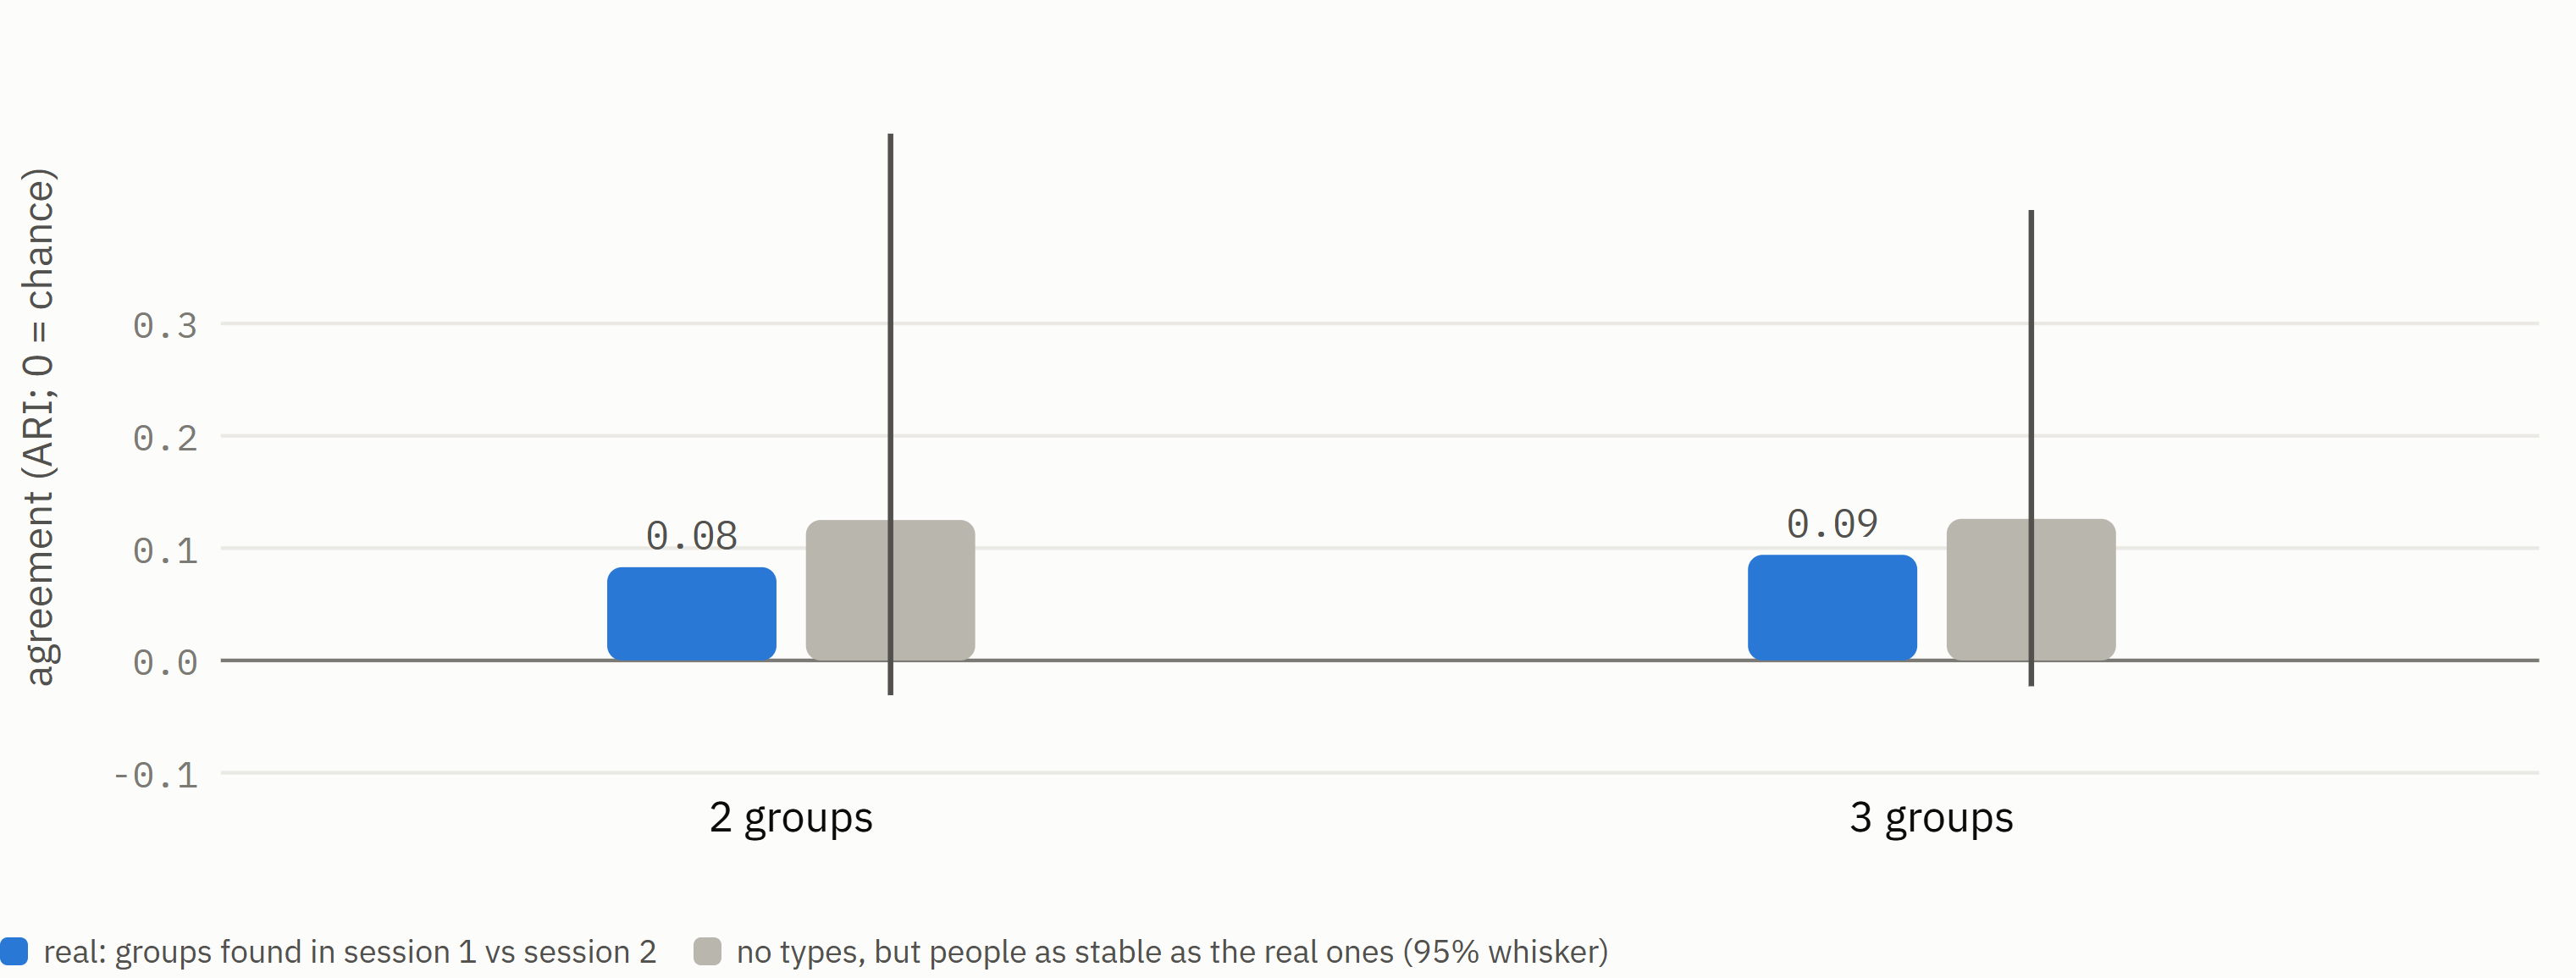
\includegraphics[width=\linewidth,height=0.24\textheight,keepaspectratio]{figs/results/f-personal-style__not-types__recur.png}\par{\scriptsize Other view: Recurrence of groupings across sessions (adjusted Rand index).}\end{minipage}

\noindent Key numbers:\begin{itemize}[leftmargin=1.2em,itemsep=0pt]\footnotesize
\item Separation (silhouette), real vs no-types simulations: 2 groups .17 vs .20 [.14, .31]; 3 groups .18 vs .19 [.14, .27]; 4 groups .20 vs .19 [.13, .25]; a no-types sample separates at least as well 84\%, 58\% and 26\% of the time
\item Groups in session 1 vs session 2 (ARI): 2 groups .08, 3 groups .09; a stable no-types cloud gives .13 on average (95\% of simulations $-$.03 to .47 for 2 groups, $-$.02 to .40 for 3), at least as high as the real value about 55\% of the time; shuffled labels give up to .12--.13
\item Round 1: two groups vs one, $\Delta$BIC 1.9 (needed > 10; 42\% of no-type simulations did at least as well)
\item Archetypes (extras2): three explain 46\% vs 43--59\% in the no-types continuum (p = .83); same archetype both sessions 61\% vs 30--79\% (p = .32)
\end{itemize}

\optsec{Nothing measured beforehand predicts the style} {\footnotesize [pass 5: for the paper]}

\noindent Key numbers:\begin{itemize}[leftmargin=1.2em,itemsep=0pt]\footnotesize
\item 0 of 40 tests survive Holm; 3 nominal (verification $\times$ score $\rho$ $-$.41; delegation $\times$ Suggest consulted $-$.38 and $\times$ plan kept $-$.40)
\item Chance alone gives 2.0 nominal hits on average; 3 or more in 34\% of 2000 shuffles of who-goes-with-whom; a p as small as the smallest one (.021) turns up somewhere in the grid in 51\% of shuffles
\item AIAS-4 $\times$ strategy card choice $\rho$ $-$.15; ``A human should make the final decision'' $\times$ strategy card choice $\rho$ $-$.08
\item AIAS-4 odds ratio for card taking 0.80 per SD [0.50, 1.27]; detectable only at about $\times$2
\item AIAS-4 mean 8.0 / 10 (SD 1.2); 32 of 33 from computing / engineering; detectable |$\rho$| $\geq$ .48
\end{itemize}
\end{options}

\clearpage

% ======== f-size-decides ========

\subsection{Small jobs by hand, big jobs to an assistant}\label{sec:res:size-decides}

The bigger the job, the more likely an operator was to hand it to an assistant, on both tiers. Measured the same way on both (the drones the mission needs), a strategy card was chosen on 56\% of the smallest missions and 75\% of the largest, and a tactical suggestion was requested on 54\% and 91\%. Comparing each person only with themselves, every doubling of mission size multiplied the odds of handing over by about 1.6 on the strategic tier ($\times 1.62$ [1.23, 2.15]) and 2.9 on the tactical tier ($\times 2.91$ [2.03, 4.17], both $p < .001$), and 22 of 33 people handed over more on their biggest missions than on their smallest on each tier. The rule is a sensible one: a strategy card is much quicker than building by hand on three-type missions and no quicker on one-type missions, and a tactical suggestion is not slower than a hand-built plan.

% --- f-size-decides#both (pass 5: for the paper) ---

\phantomsection\label{sec:res:size-decides:both}
Figure~\ref{fig:res:size-decides:both} shows the share of decisions handed over, on each tier, by the number of drones the mission needs. Both rise; the tactical tier rises more steeply and keeps rising. The strategic tier dips at five drones: these are seven particular one-type missions in the two Strategic Heavy games, six of which arrived in bursts, so operators reached them with three or four other missions waiting and often decided before the cards had loaded. Participants described the rule in their own words, for example: ``I think if it's just one colour, I'm gonna do it, like, assign it myself, but if it's multiple colours, I think I'm gonna let, um, the AI choose for me, for the, the strategic side'' (P29), and ``When they only needed a single colour of drone I tended to do it manually'' (P34).

\begin{figure}[H]
\centering
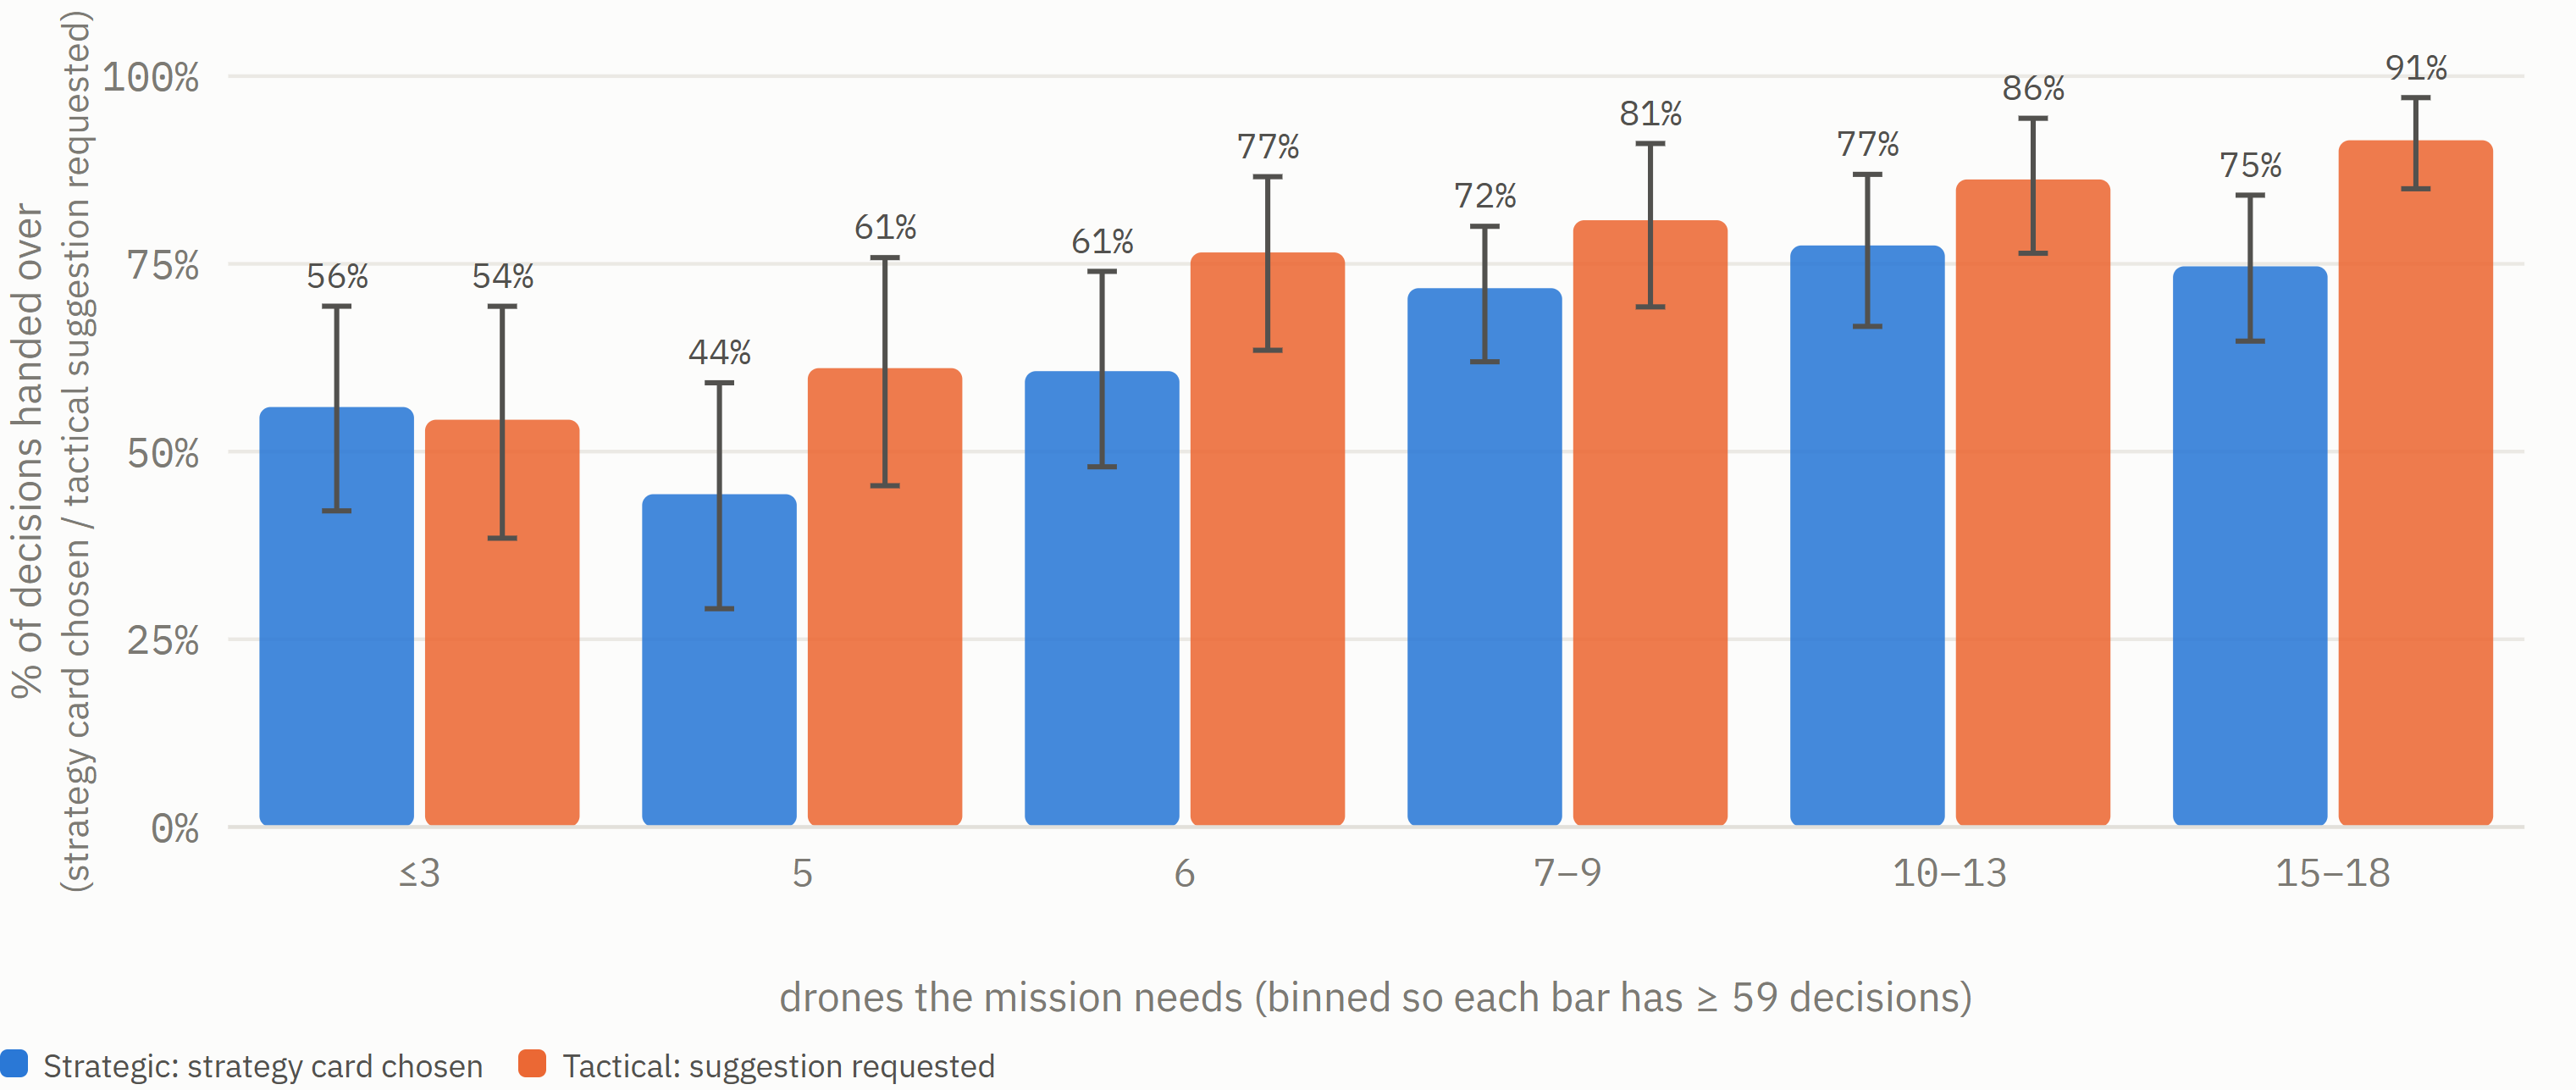
\includegraphics[width=\linewidth,height=0.50\textheight,keepaspectratio]{figs/results/f-size-decides__both__main.png}
\caption{\textbf{The bigger the mission, the more it is handed to an assistant, on both tiers.} Share of decisions where a strategy card was chosen (blue) or a tactical suggestion requested (orange), by the drones the mission needs; whiskers are 95\% intervals.}
\label{fig:res:size-decides:both}
\end{figure}

% --- f-size-decides#models (pass 5: for the paper) ---

\phantomsection\label{sec:res:size-decides:models}
The effect holds when each person is compared only with themselves, for every way of measuring size and on both tiers (Figure~\ref{fig:res:size-decides:models}). Dropping every illogical Conservative card leaves it in place (strategic $\times 1.46$ per doubling, $p = .006$), as does allowing for every operator having played the same fixed missions (strategic $\times 1.60$, tactical $\times 2.89$, both $p \leq .001$). With each mission as a single point, the share handed over still rises with its size ($\rho = .63$ on the strategic tier and $.69$ on the tactical, 41 missions each).

\begin{figure}[H]
\centering
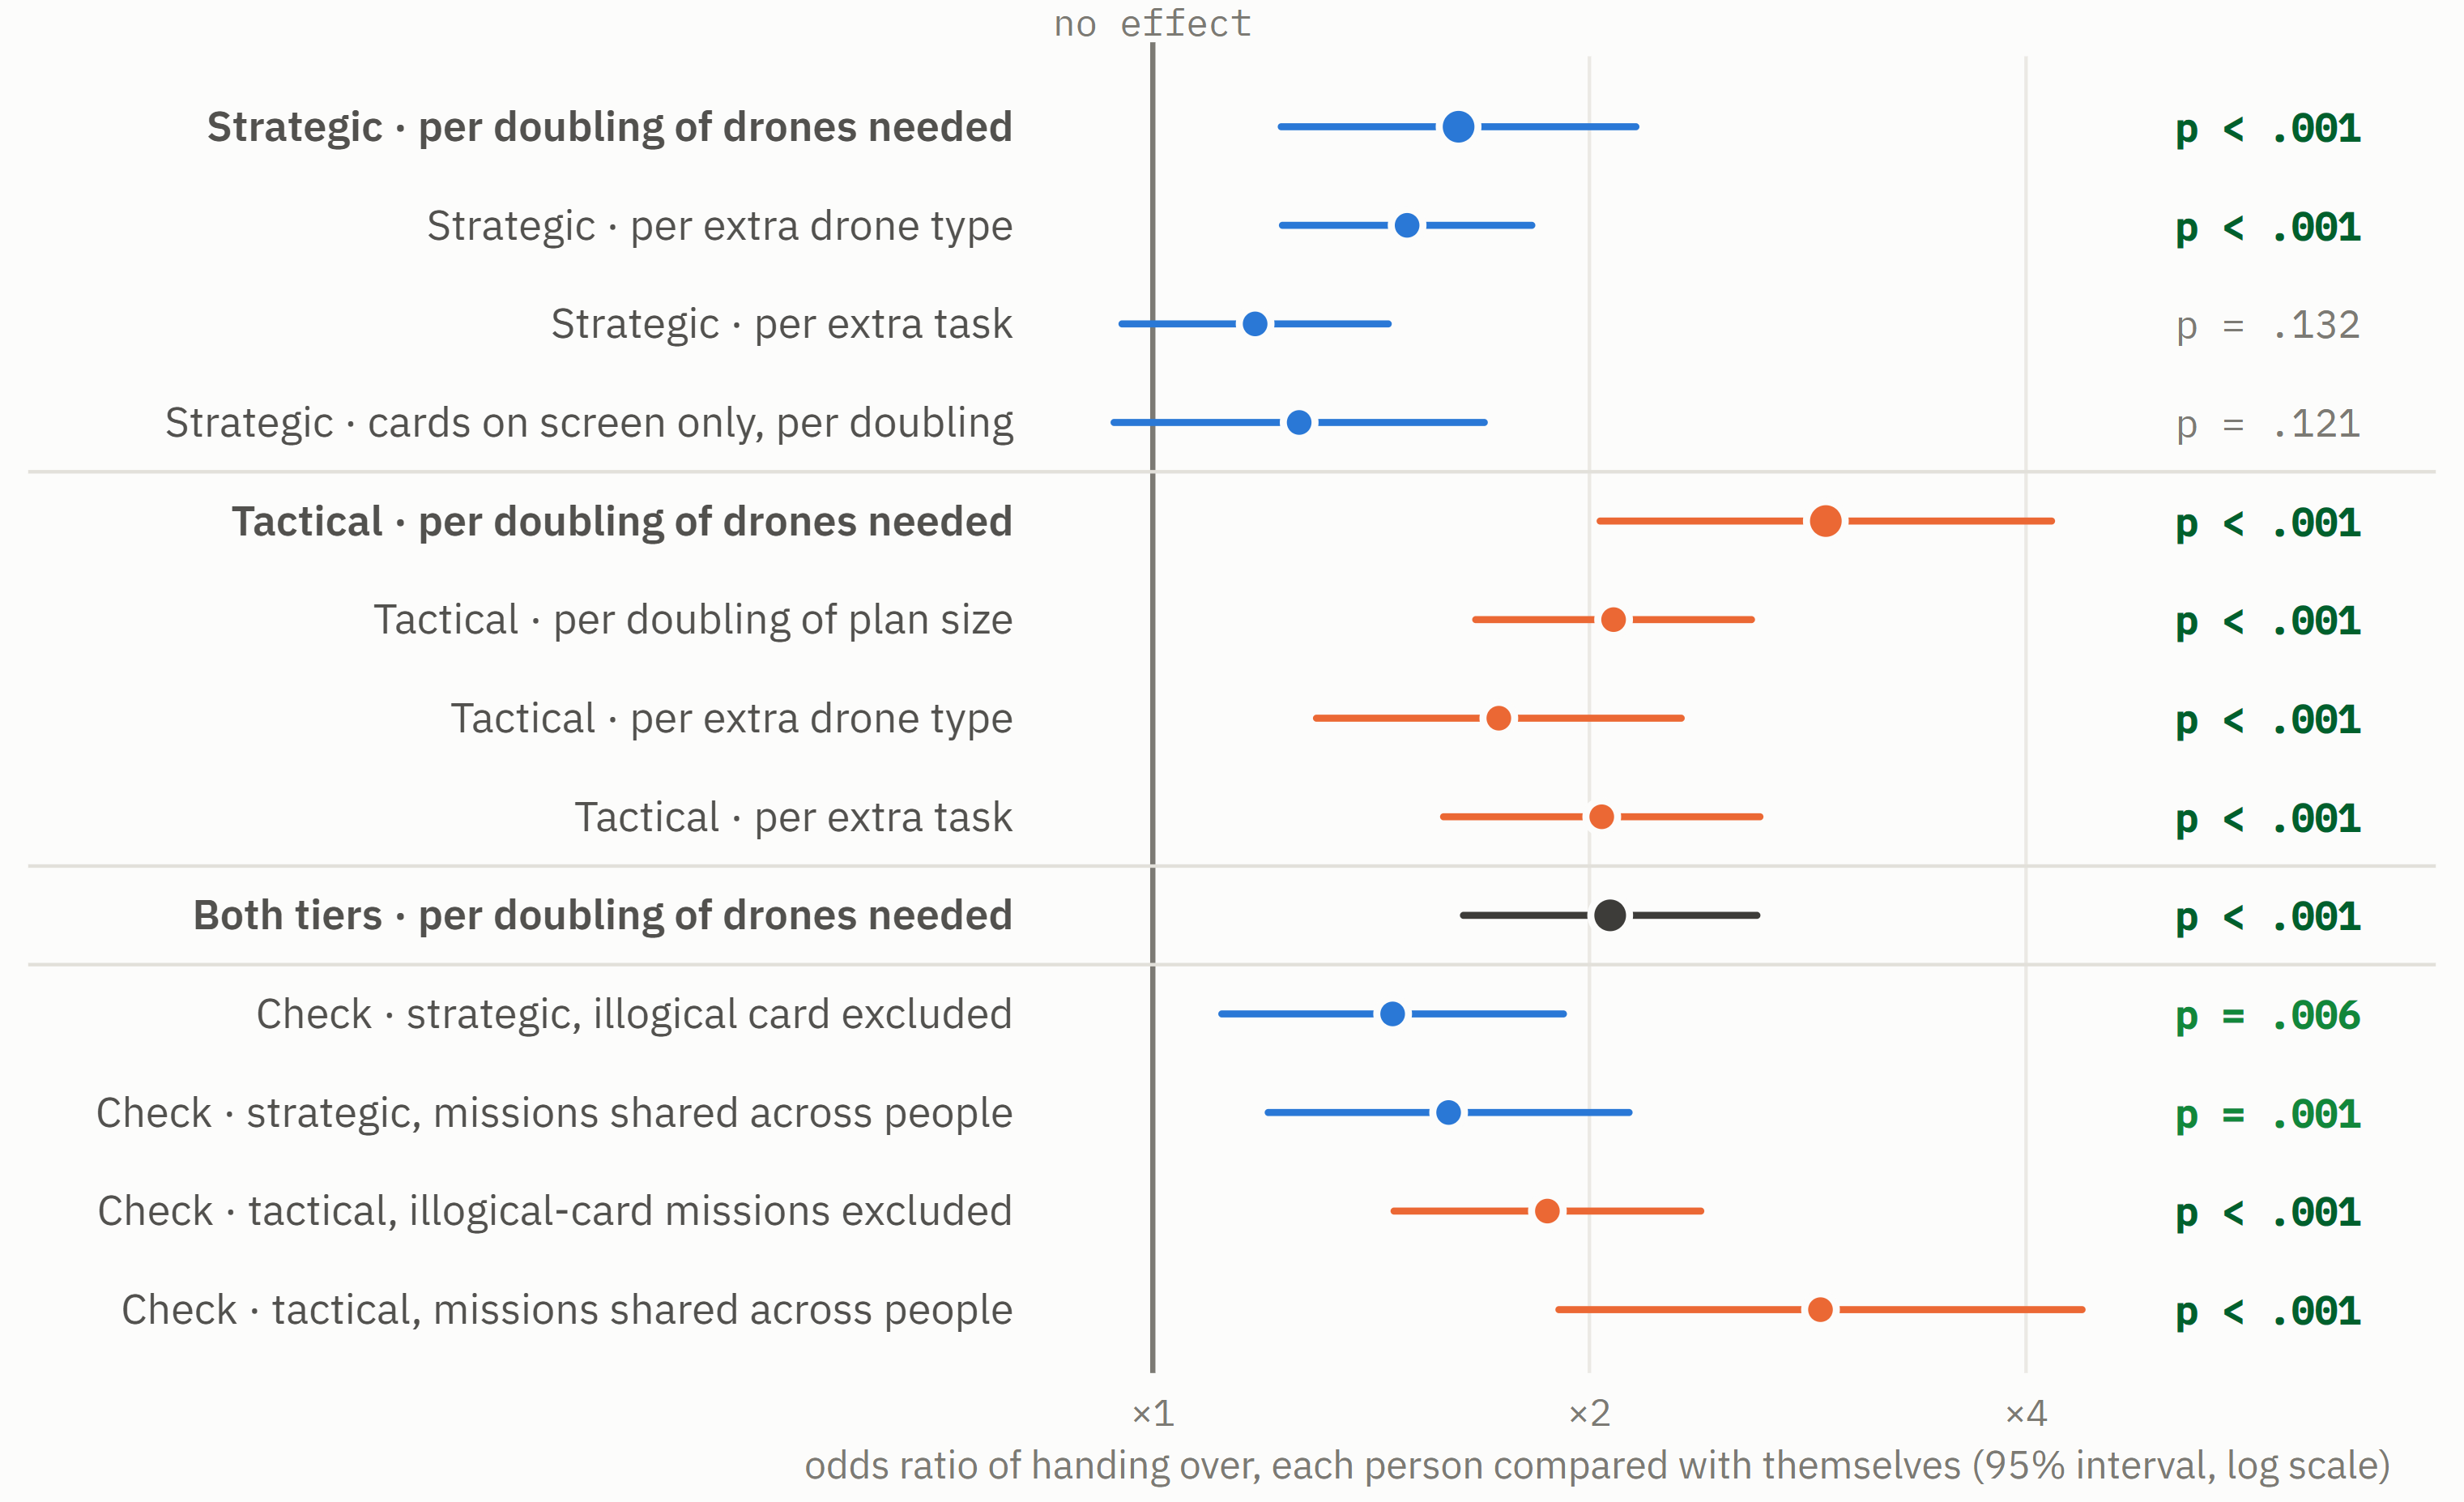
\includegraphics[width=\linewidth,height=0.50\textheight,keepaspectratio]{figs/results/f-size-decides__models__main.png}
\caption{\textbf{Bigger jobs are handed over more, for every size measure and on both tiers.} Each row is a within-person odds ratio per unit of size with its 95\% interval; the bottom block holds the checks for artefacts.}
\label{fig:res:size-decides:models}
\end{figure}

% --- f-size-decides#tactical (pass 5: for the paper) ---

\phantomsection\label{sec:res:size-decides:tactical}\label{sec:res:size-decides:route-people}
The two tiers are also linked. A mission whose drones came from a strategy card was more likely to get a tactical suggestion than one allocated by hand, at every size (Figure~\ref{fig:res:size-decides:tactical:needed}): for the same person and mission size, about twice the odds ($\times 2.10$ [1.30, 3.40], $p = .003$). The gap is wide on small missions (70\% against 35\% at three drones or fewer) and narrow on the largest (93\% against 88\%), but that narrowing is both rates approaching 100\% rather than a reliable change. It is a general tendency rather than the habit of a few people: of the 26 who did both often enough to compare, 17 leaned this way and 8 the other, although the three largest gaps make up about half of the total. Participants described the same continuity: ``Now I'm using the suggestion because I took the aggressive approach which means I know that I have enough drones'' (P10). Size also mattered in plain practical terms: ``If I look at a mission with 15 drones and I need to move two or three chains, that's just going to take me about a minute, and it's just no point'' (P11).

\begin{figure}[H]
\centering
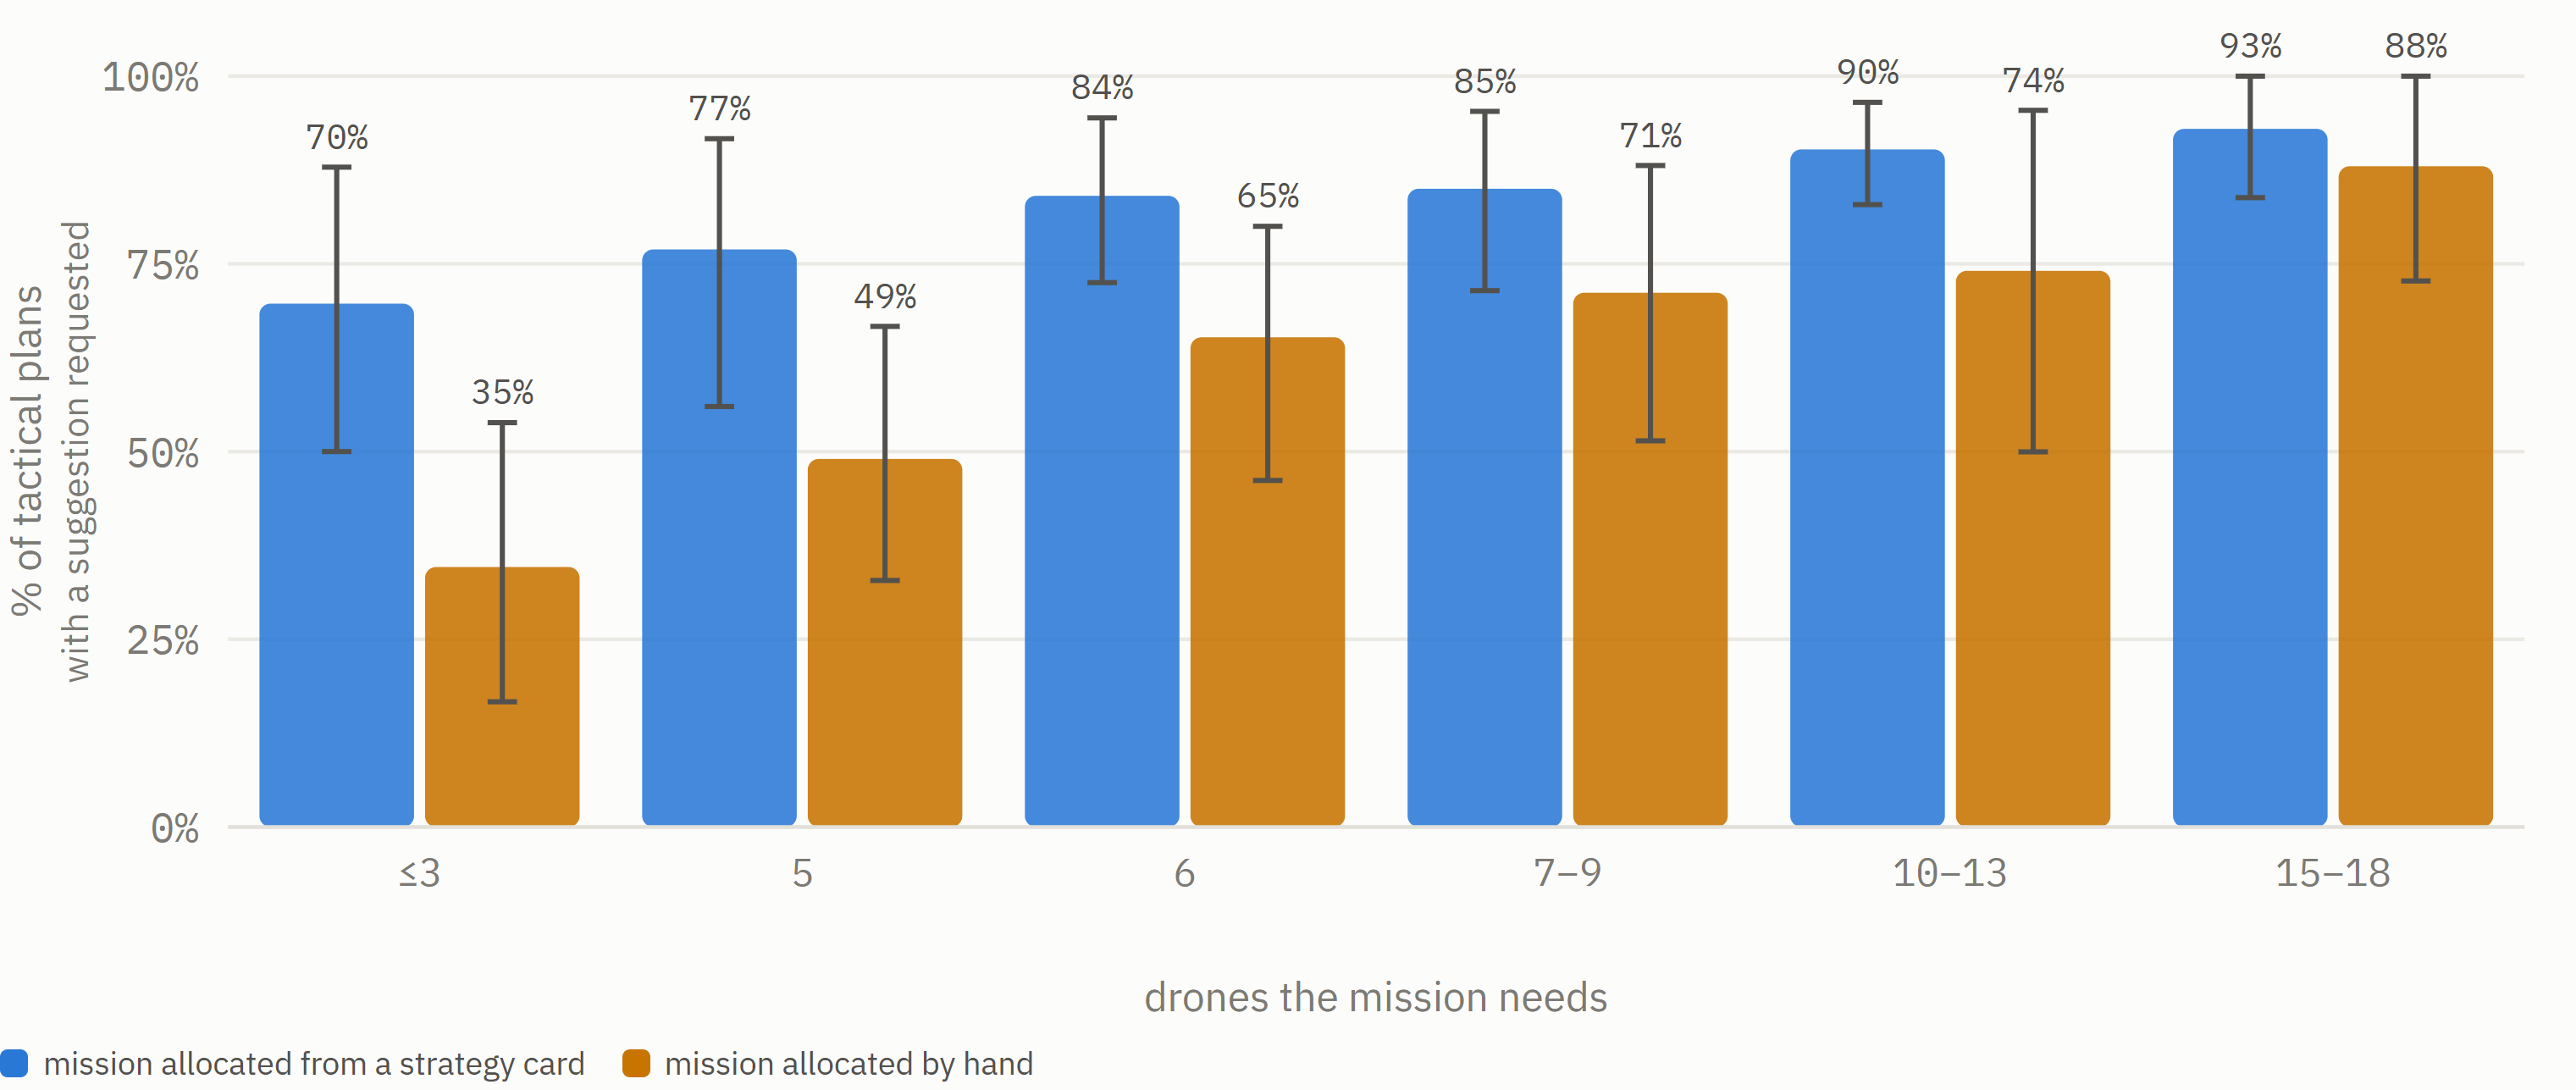
\includegraphics[width=\linewidth,height=0.50\textheight,keepaspectratio]{figs/results/f-size-decides__tactical__needed.png}
\caption{\textbf{A mission allocated from a strategy card is more likely to get a tactical suggestion.} Share of tactical plans with a suggestion requested, by the drones the mission needs, split by how the mission was allocated.}
\label{fig:res:size-decides:tactical}
\label{fig:res:size-decides:tactical:needed}
\end{figure}

% --- f-size-decides#speed (pass 5: extra: may make it in) ---

\phantomsection\label{sec:res:size-decides:speed}
The size rule also fits the time each route takes (Figure~\ref{fig:res:size-decides:speed}). On the strategic tier, choosing a strategy card is much quicker than building by hand on three-type missions (27\% less time for the same person, $p < .001$) and no quicker on one-type missions ($+22\%$, $p = .09$); with the idle time before the first click removed, the card is 44\% quicker on three-type missions and level on one-type ones. On the tactical tier, hand-built plans and tactical suggestions take about the same planner time (29 against 27\,s on average), within a second of each other for the same person and mission size. Speed was the most common reason participants gave for using the assistants: ``The top advantage in this situation was the speed of response'' (P31).

\begin{figure}[H]
\centering
\begin{subfigure}[t]{0.495\linewidth}
\centering
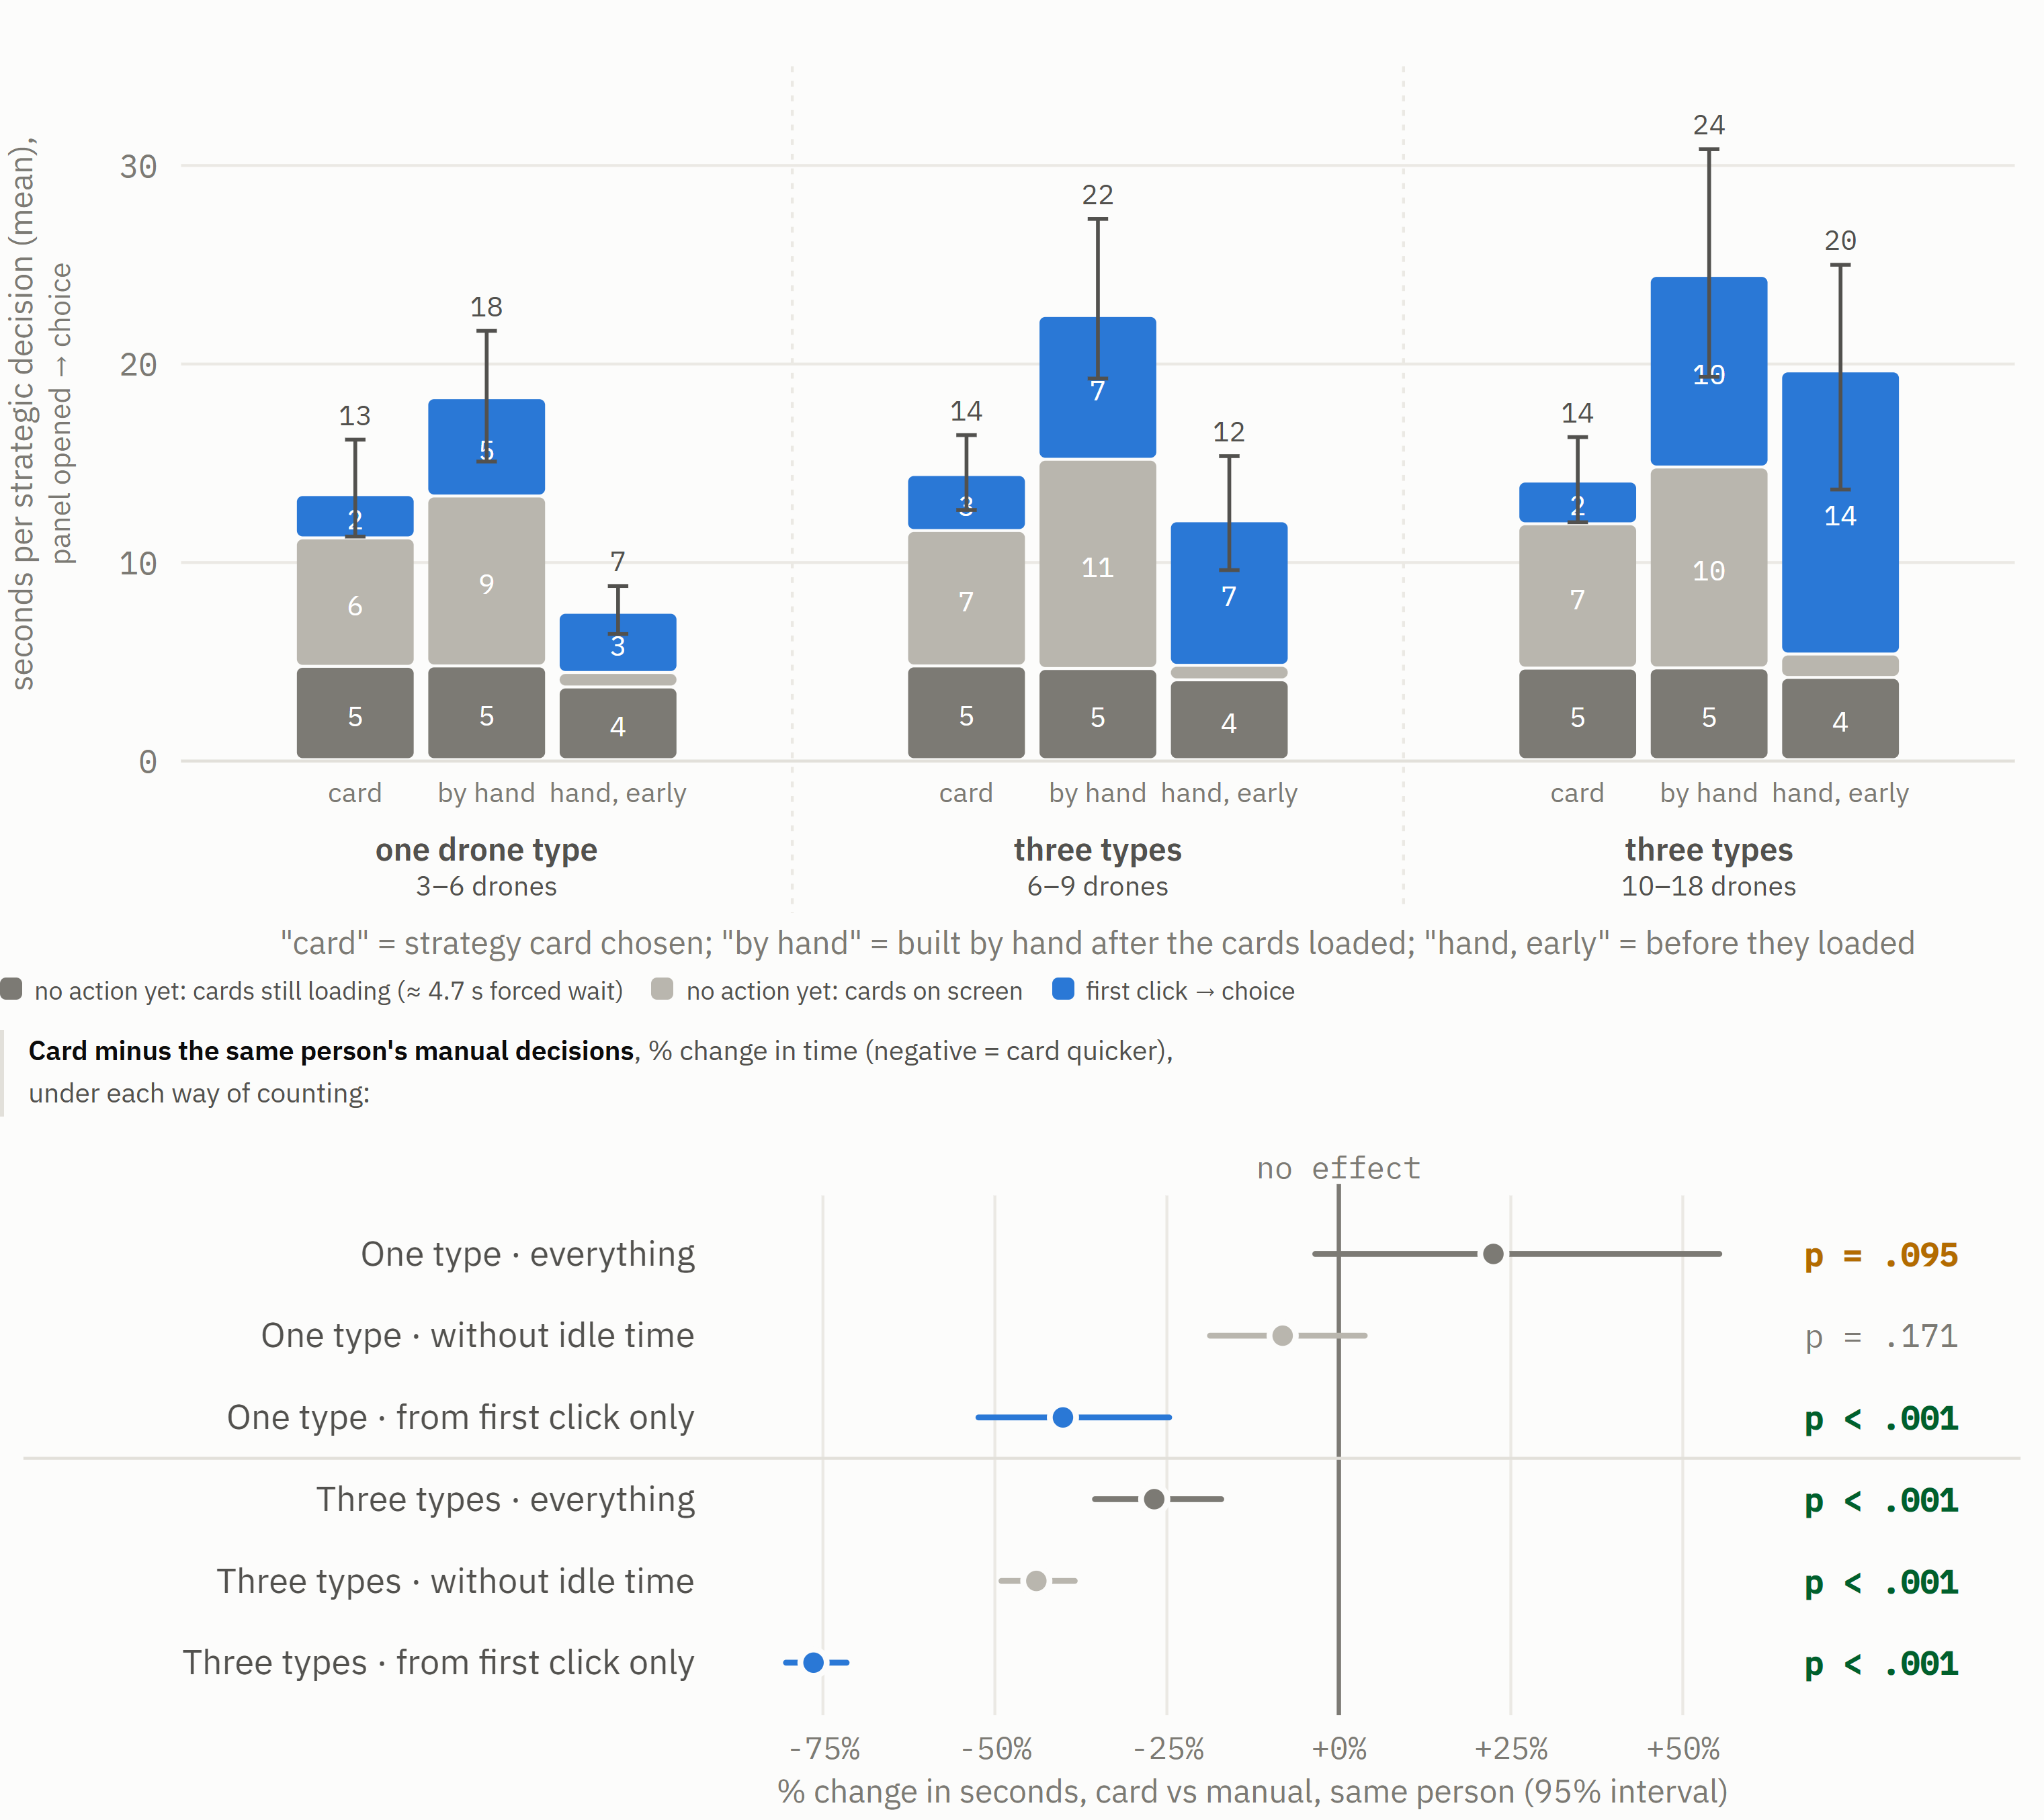
\includegraphics[width=\linewidth,height=0.55\textheight,keepaspectratio]{figs/results/f-size-decides__speed__strat-all.png}
\caption{Strategic tier, all time counted.}
\label{fig:res:size-decides:speed:strat-all}
\end{subfigure}
\hfill
\begin{subfigure}[t]{0.495\linewidth}
\centering
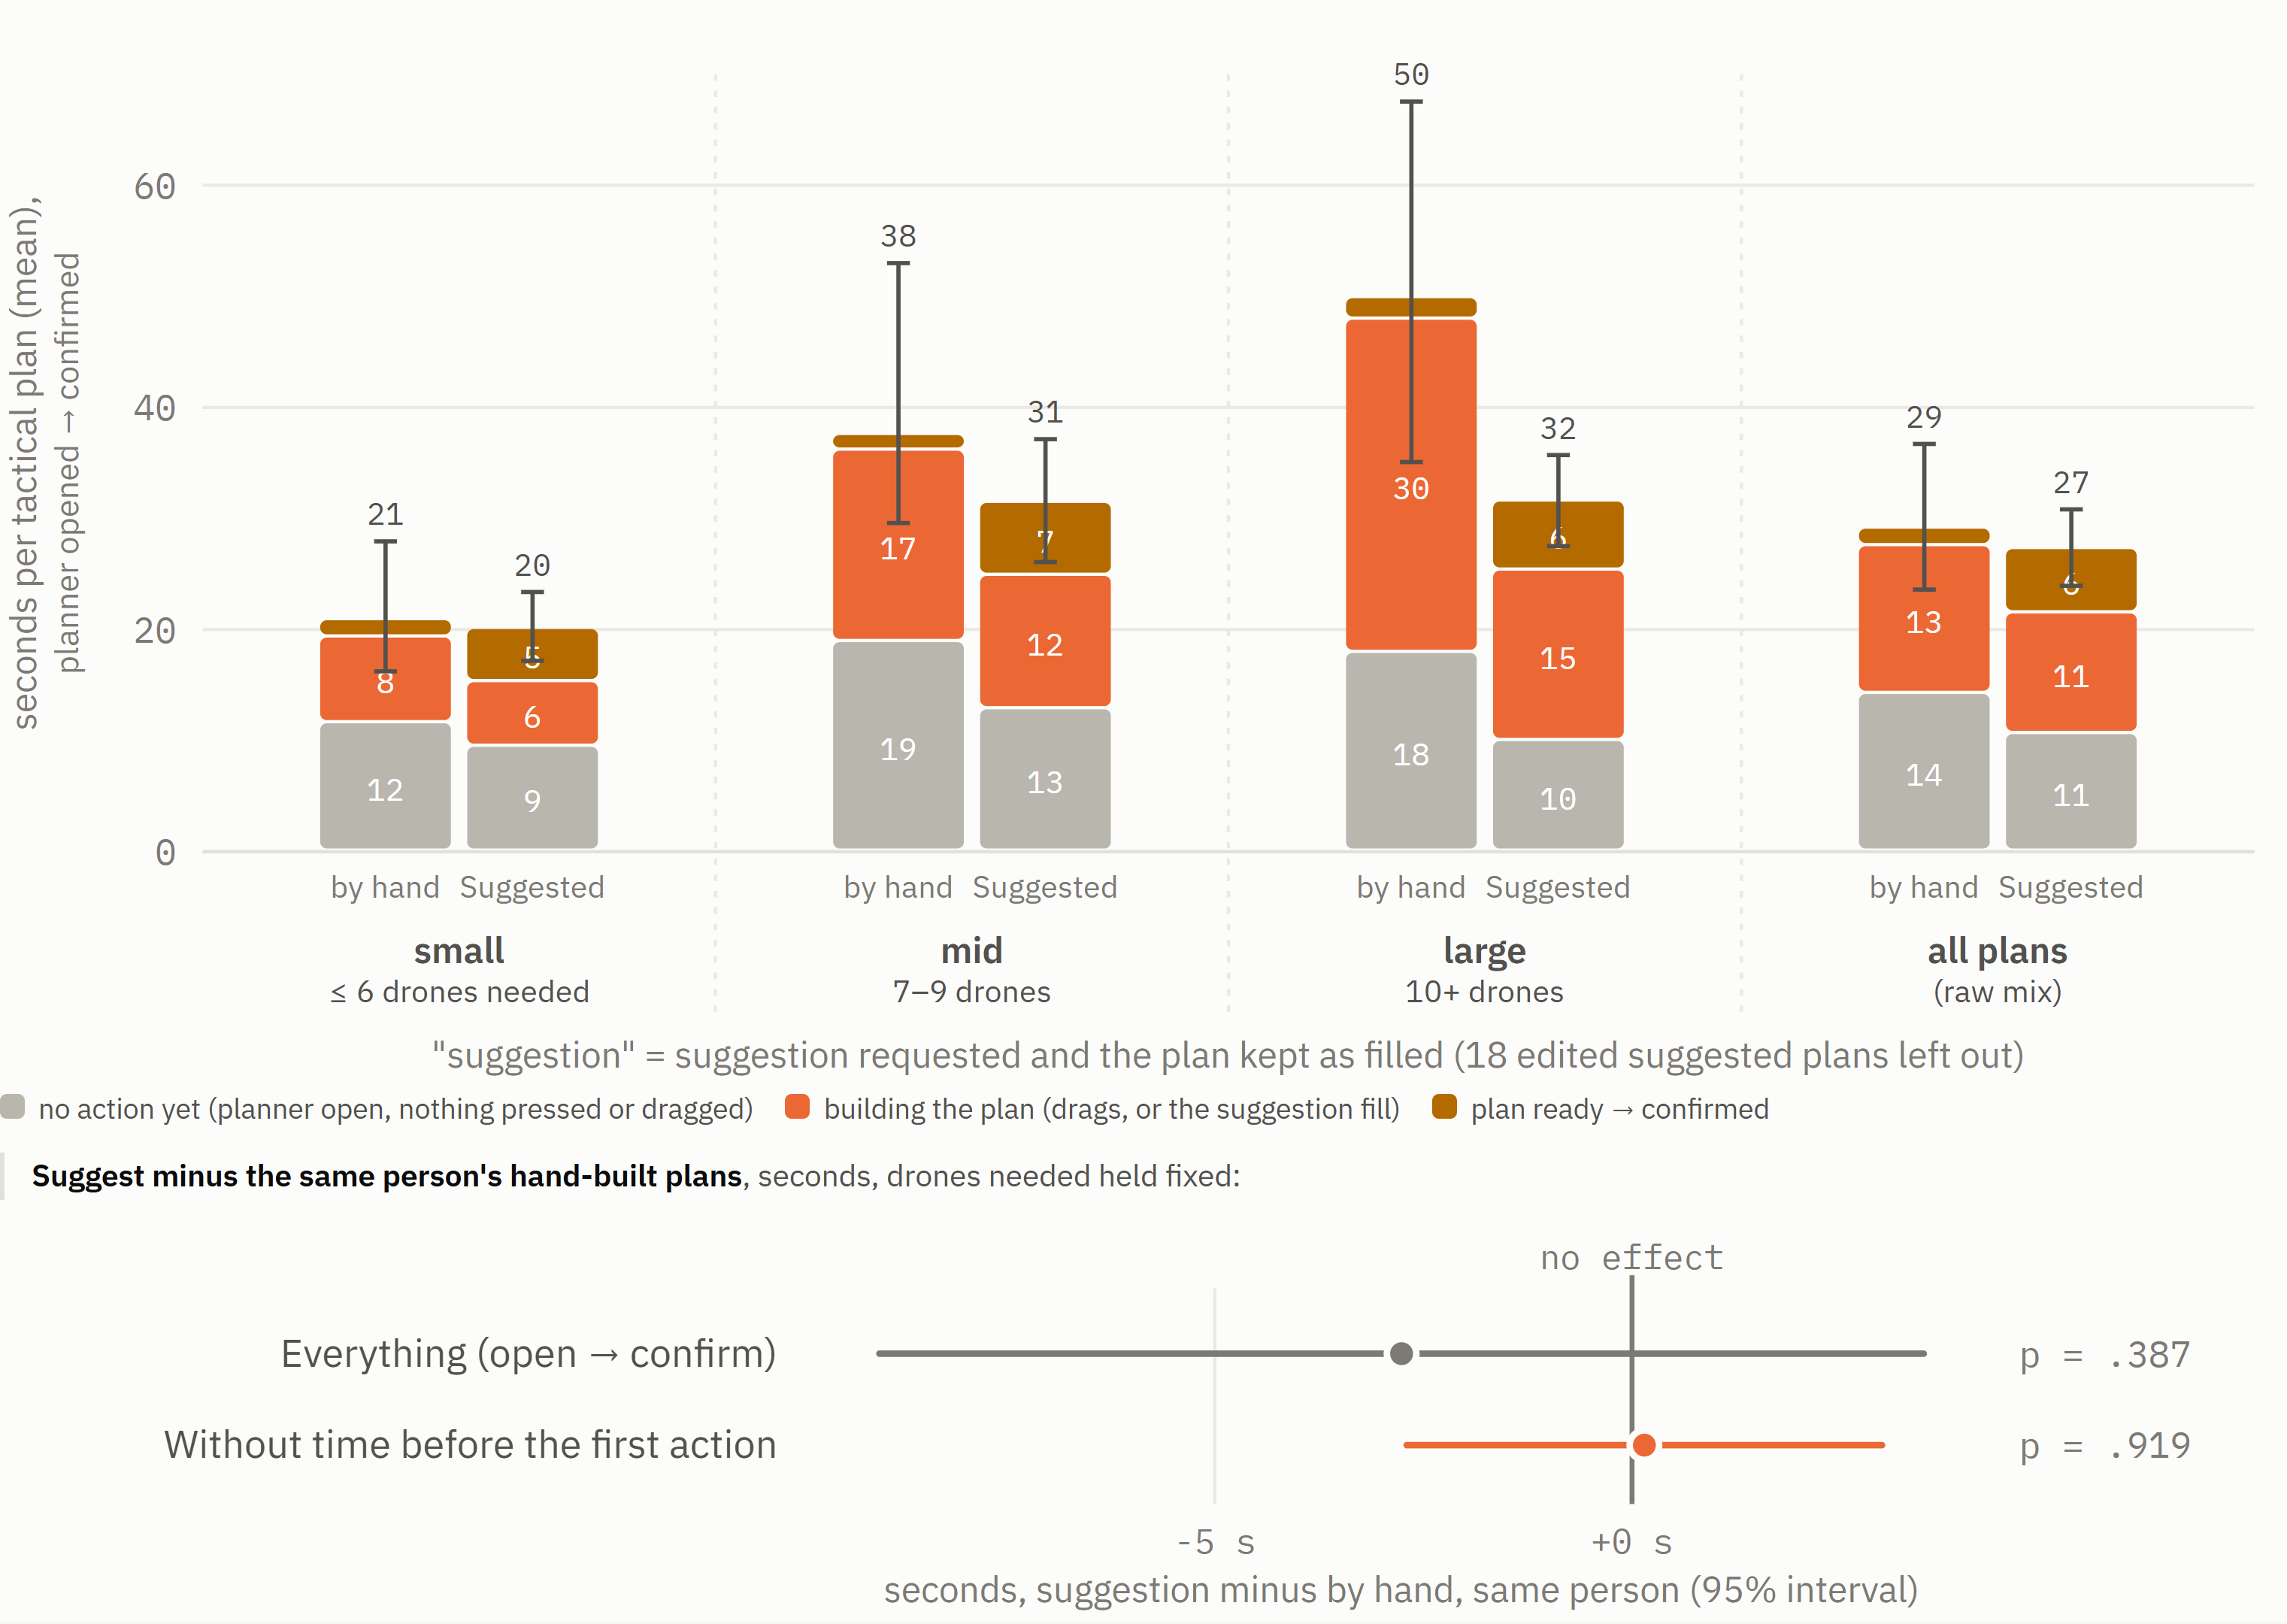
\includegraphics[width=\linewidth,height=0.55\textheight,keepaspectratio]{figs/results/f-size-decides__speed__tac-all.png}
\caption{Tactical tier, all time counted.}
\label{fig:res:size-decides:speed:tac-all}
\end{subfigure}
\par\smallskip
\caption{\textbf{A strategy card saves time only on big strategic jobs; a tactical suggestion saves no planner time.} Each decision's time split into the time before the operator's first action and after it, by mission size: (a) strategic tier, (b) tactical tier.}
\label{fig:res:size-decides:speed}
\end{figure}

% --- f-size-decides#parallel (pass 5: for the paper) ---

\phantomsection\label{sec:res:size-decides:parallel}
Where a tactical suggestion does gain is in carrying the plan out (Figure~\ref{fig:res:size-decides:parallel:all}). Splitting each tactical plan into four phases, the operator's own time is the same either way: a suggestion saves about 3\,s in building the plan and gives it back between the plan being ready and being confirmed. The only reliable difference is that a suggested plan is carried out about 11\,s sooner ($p = .006$), roughly a tenth of a mission. The common feeling that the assistant is faster is therefore only weakly supported: it does not save the operator time, and its plans finish a little sooner. Nor does relying on the assistants more make an operator do better: within a person, missions allocated from a strategy card were completed in full no more often than their own hand-built ones (60\% against 62\%, $p = .27$).

\begin{figure}[H]
\centering
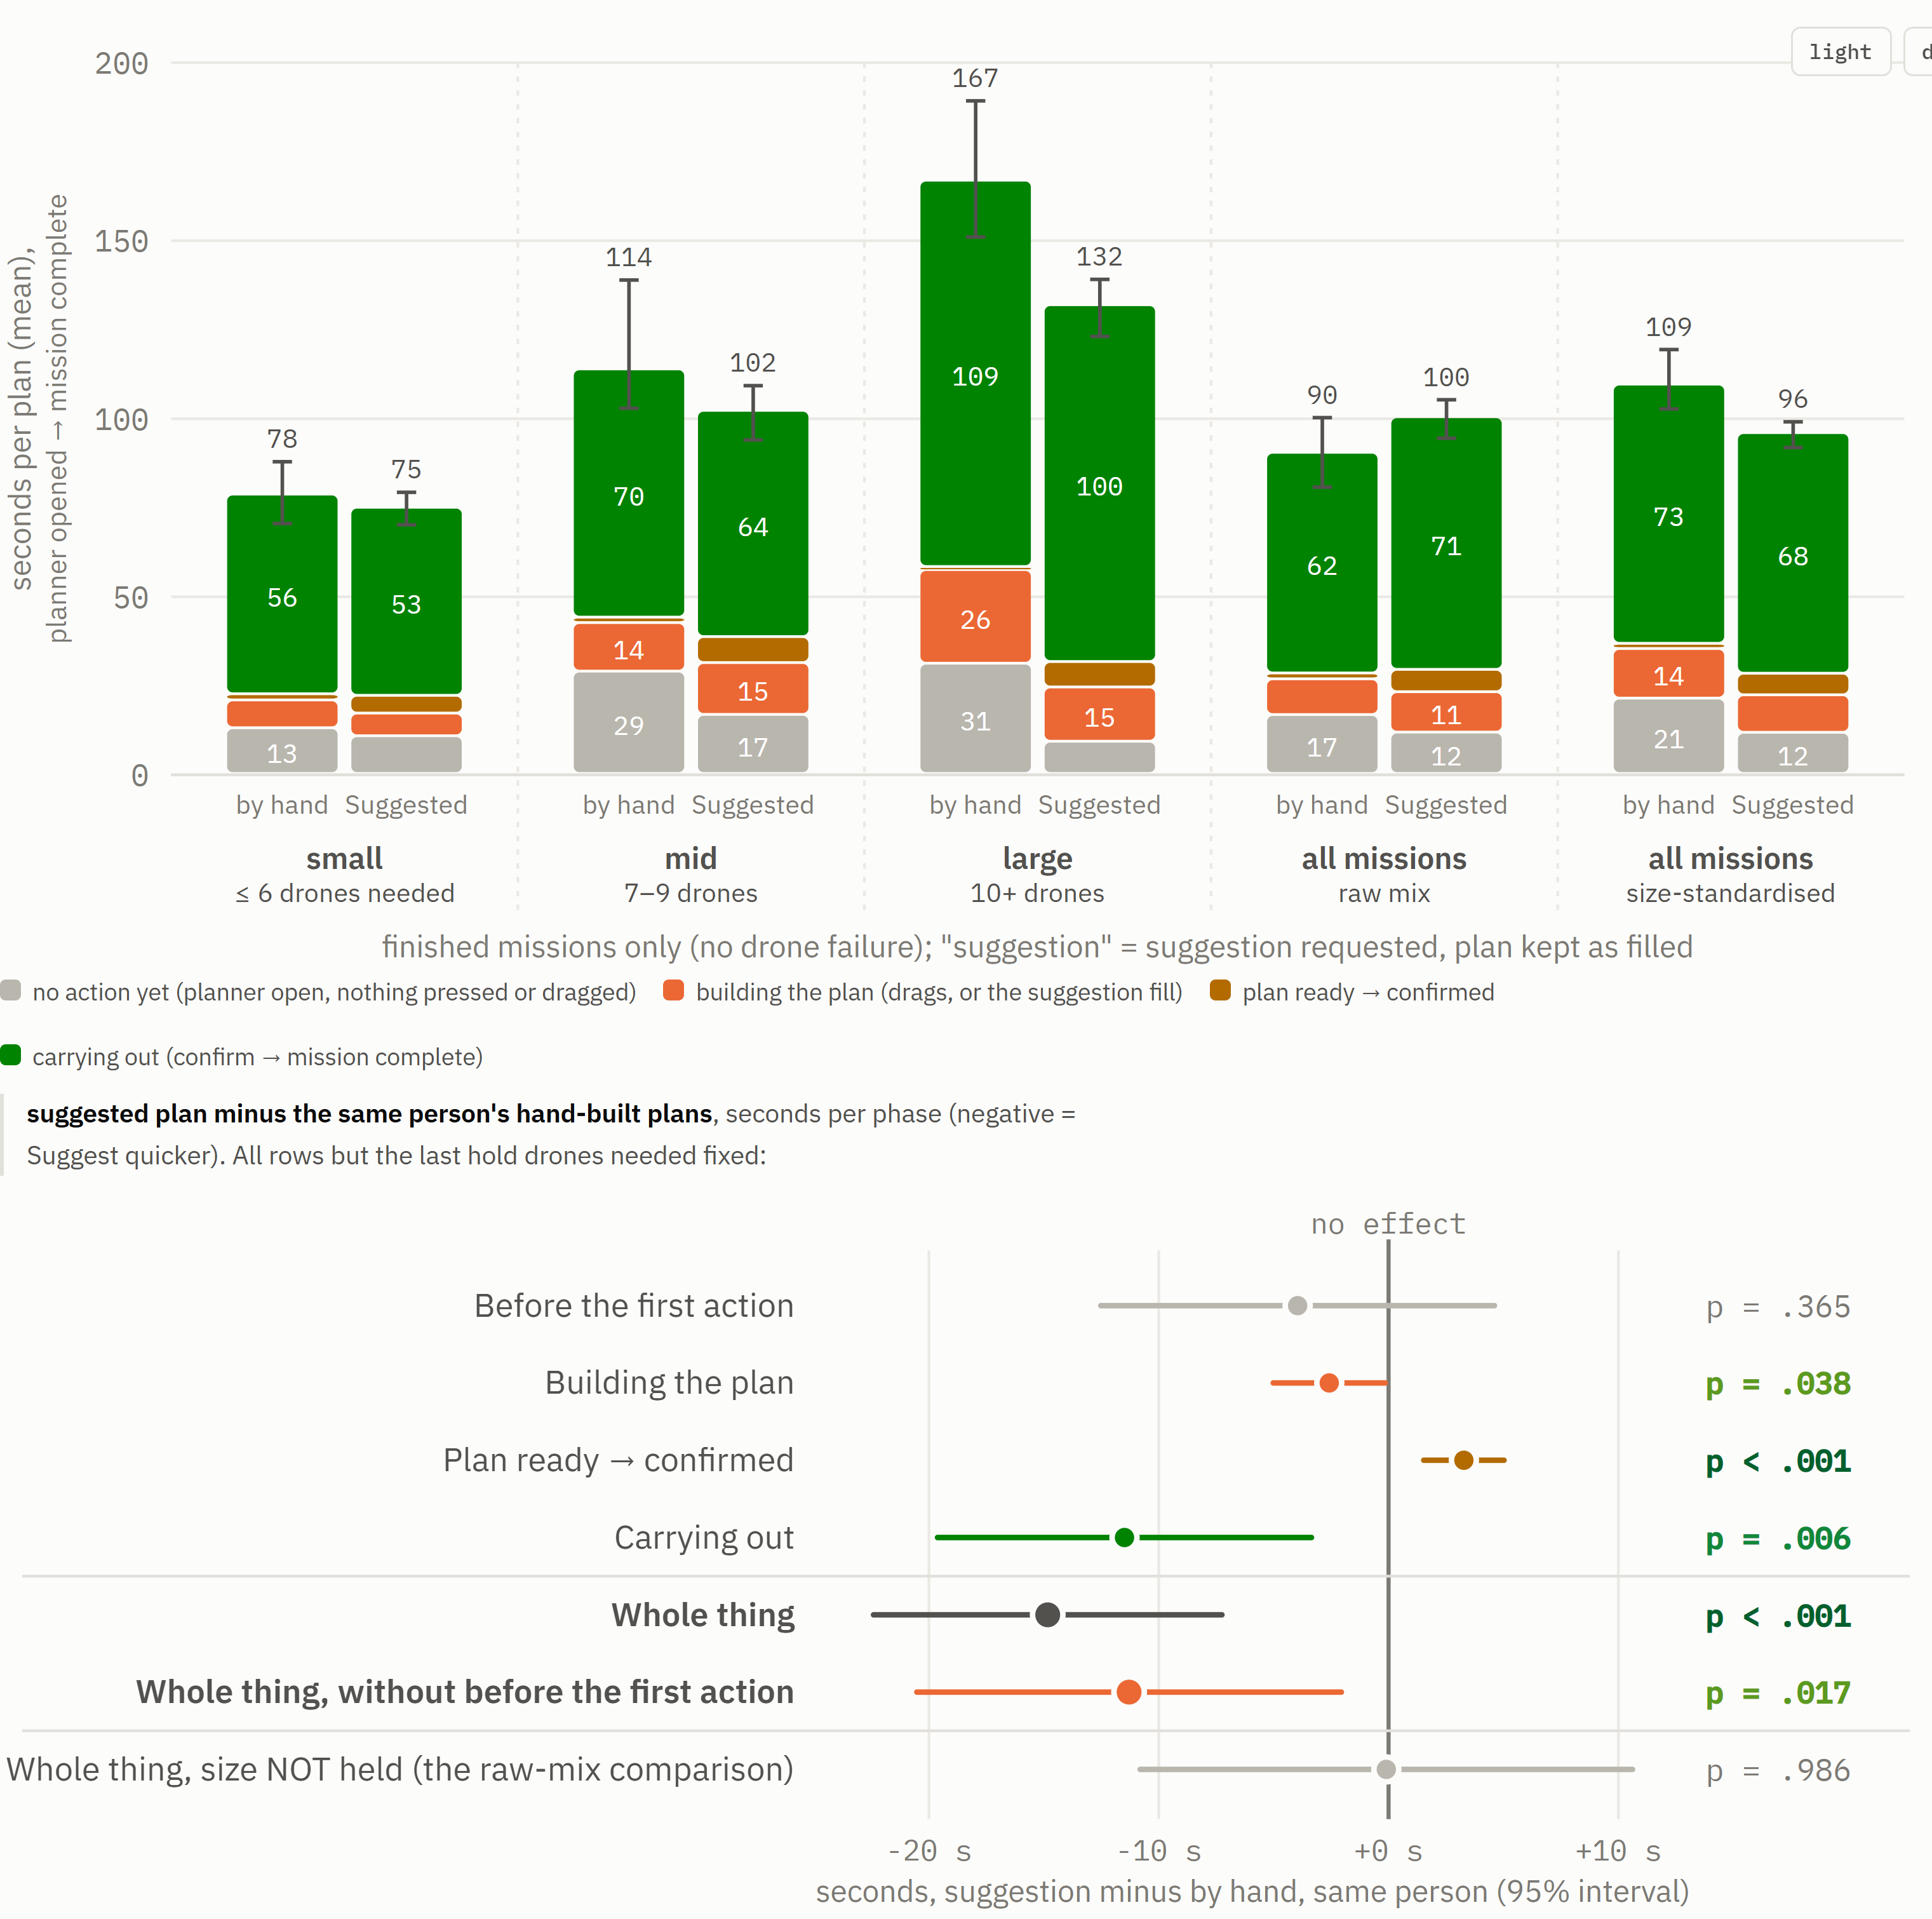
\includegraphics[width=\linewidth,height=0.50\textheight,keepaspectratio]{figs/results/f-size-decides__parallel__all.png}
\caption{\textbf{Hand-built and suggested tactical plans take the operator about the same time; suggested plans are carried out a little sooner.} Mean time per tactical plan in four phases, by mission size.}
\label{fig:res:size-decides:parallel}
\label{fig:res:size-decides:parallel:all}
\end{figure}

% --- f-size-decides#said (pass 5: for the paper) ---

\phantomsection\label{sec:res:size-decides:said}\label{sec:res:size-decides:parallel-said}
Ten of 33 participants stated the size rule without being asked, and 15 valued the assistants for speed rather than accuracy. Several also described using the wait: while a suggestion filled in, they turned to the next mission. The logs agree: 45\% of tactical plans with a suggestion requested had another mission's strategic panel opened while the planner was open, against 19\% of hand-built plans.

\begin{options}
\optshead{Options for this finding}

\optsec{Both tiers on one axis: the bigger the mission, the more it is handed over} {\footnotesize [pass 5: for the paper]}

\noindent Key numbers:\begin{itemize}[leftmargin=1.2em,itemsep=0pt]\footnotesize
\item Strategic, per doubling of drones needed: odds $\times$1.62 [1.23, 2.15], p < .001 (606 decisions, 33 people)
\item Tactical, per doubling of drones needed: odds $\times$2.91 [2.03, 4.17], p < .001 (627 plans)
\item Both tiers, one shared slope: $\times$2.07 [1.64, 2.61], p < .001 (1,233 decisions); the tactical slope is steeper than the strategic one by $\times$1.38 [0.99, 1.91], p = .056 --- suggestive, not shown
\item Raw rates, smallest to largest bin: strategic 56\% $\rightarrow$ 75\%, tactical 54\% $\rightarrow$ 91\%
\item Arrival bursts (Strategic Heavy games, fixed per game): the seven 5-drone missions had on average 4.4 other missions arrive within 60 s of them, against 3.6 for the 3- and 6-drone one-type missions and 3.1 for every other mission; 6 of 7 arrived inside or straight after a burst; the seventh arrived 10 s into a game and got the card 69\% of the time
\end{itemize}

\noindent Highlighted quotes not used above:\begin{quotelist}
\item ``either it's a really big mission, and it's like, oh, I can trust it with a large mission. [\ldots{}] Or it's a simple mission, and I'll be like, oh, I can just bang it up myself.''\,---\,P11 (debrief 0:28:41)
\item ``I did feel like some of them I should do myself and I trusted it more with the complicated tasks''\,---\,P29 (debrief 0:24:54)
\item ``I'll use the suggest, because there's a lot of drones here, so because there's a lot of drones to allocate''\,---\,P05 (think-aloud s1 0:09:36)
\end{quotelist}

\optsec{Person-adjusted: every size measure, both tiers, one picture} {\footnotesize [pass 5: for the paper]}

\noindent Key numbers:\begin{itemize}[leftmargin=1.2em,itemsep=0pt]\footnotesize
\item Strategic, illogical Conservative card excluded: $\times$1.46 [1.12, 1.92], p = .006 (474 decisions)
\item Missions shared across people (interval clustered on person and mission): strategic $\times$1.60 [1.20, 2.13], p = .001; tactical $\times$2.89 [1.91, 4.37], p < .001 (65 missions)
\item Each mission as one point (missions with $\geq$ 5 decisions): strategic $\rho$ = .63 over 41 missions, tactical $\rho$ = .69 over 41 (both p < .001)
\end{itemize}

\optsec{Tactical tier: Suggest rises with mission size, and goes with the strategic choice} {\footnotesize [pass 5: for the paper]}

\par\noindent \begin{minipage}[t]{0.49\linewidth}\centering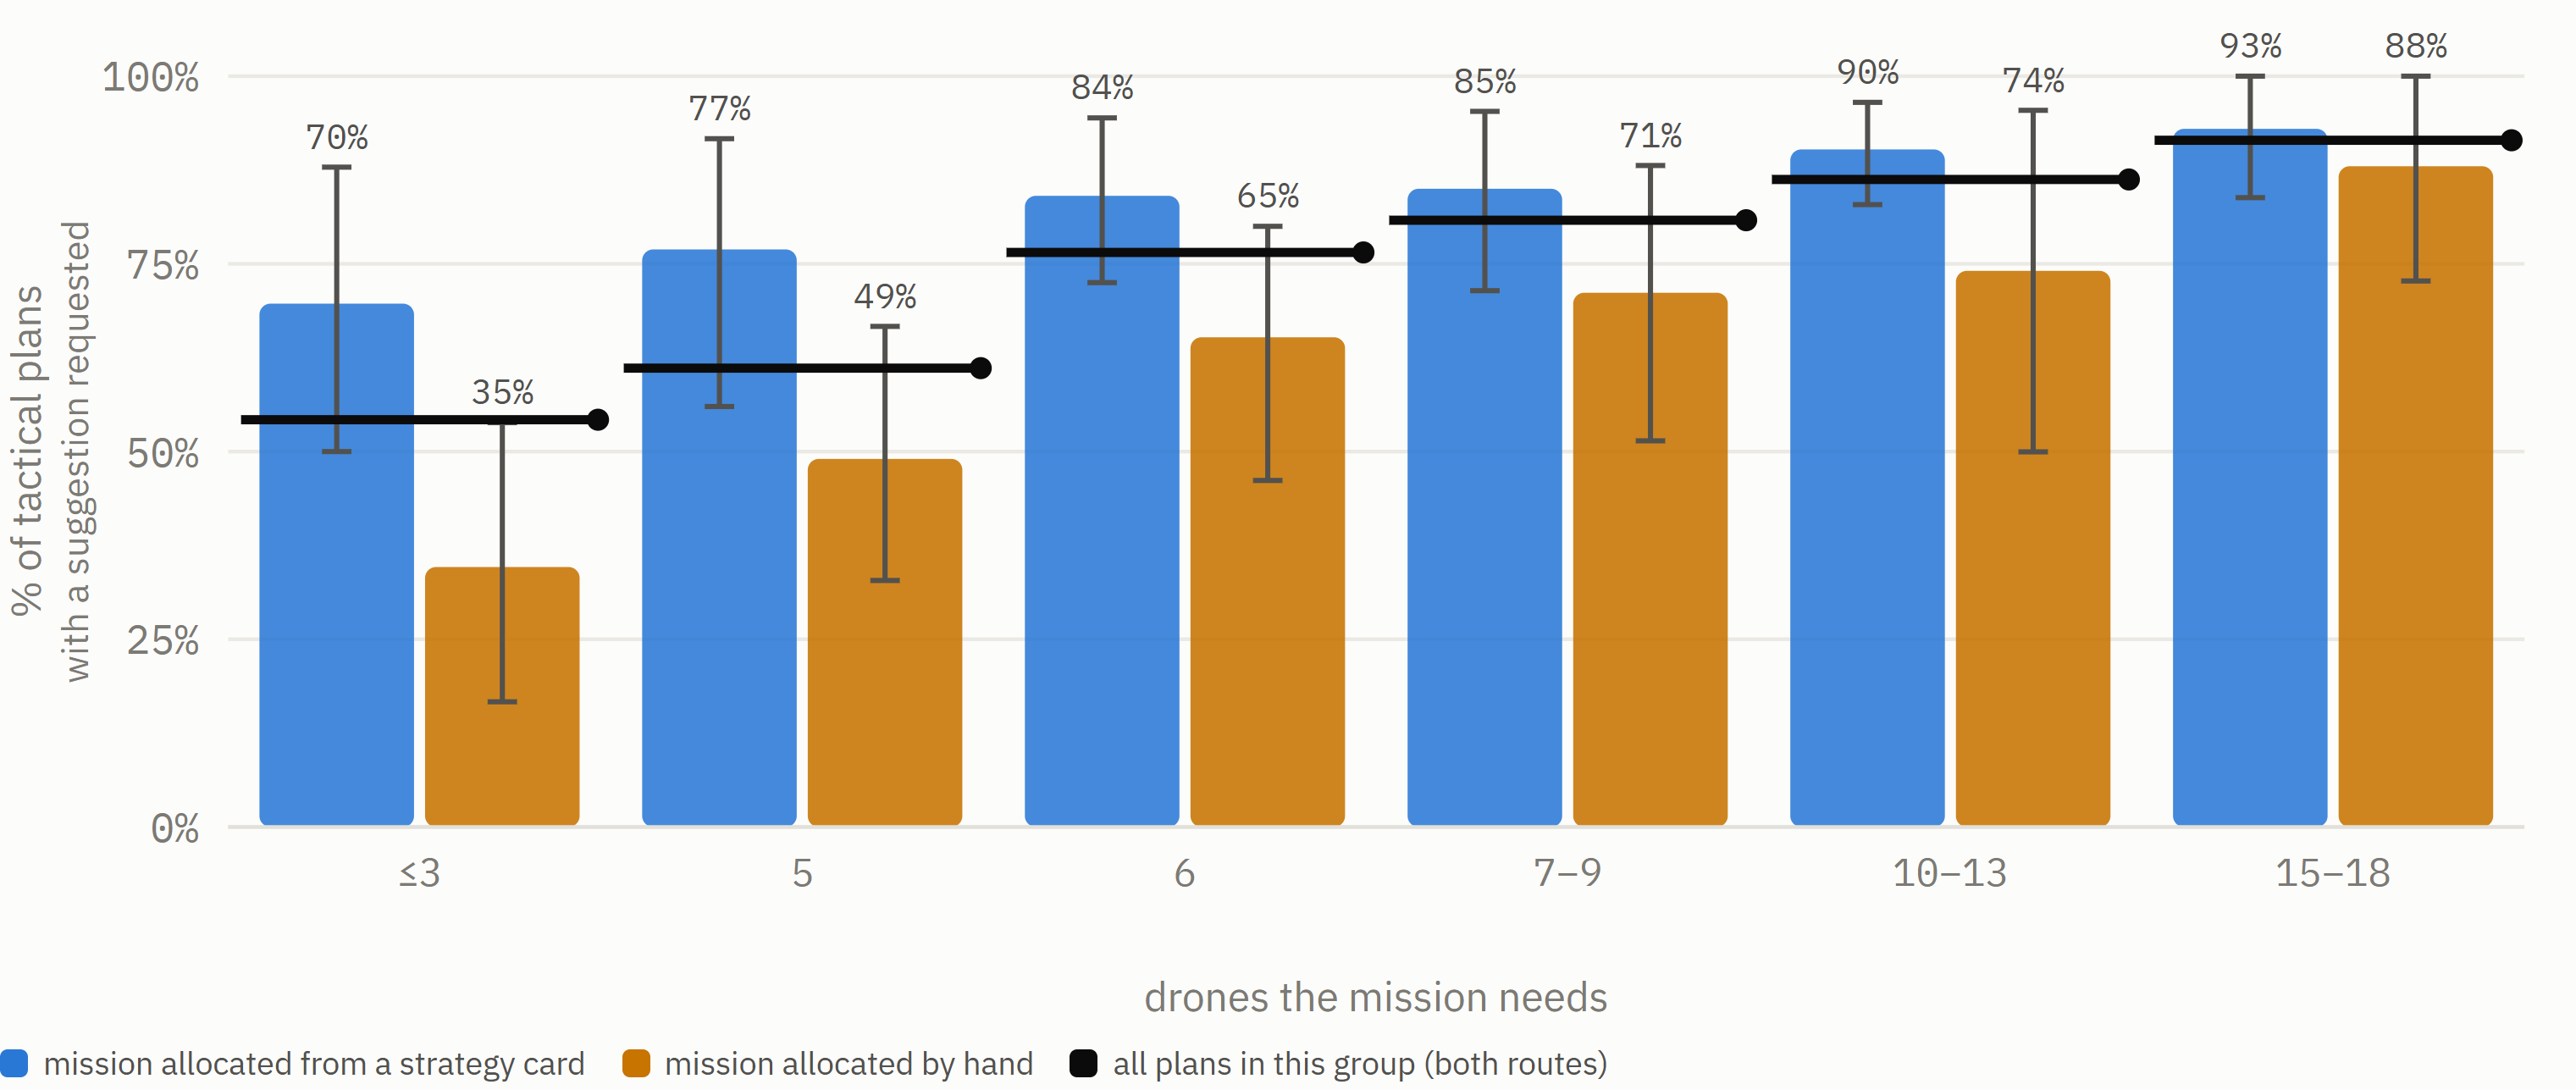
\includegraphics[width=\linewidth,height=0.24\textheight,keepaspectratio]{figs/results/f-size-decides__tactical__marker.png}\par{\scriptsize Other view: With a marker on each pair at the rate for all plans in that size group.}\end{minipage}

\noindent Key numbers:\begin{itemize}[leftmargin=1.2em,itemsep=0pt]\footnotesize
\item Within person, per doubling of drones needed: odds $\times$2.91 [2.03, 4.17]; per extra task $\times$2.04 [1.59, 2.62]; per extra drone type $\times$1.73 [1.30, 2.31]; per doubling of drones committed $\times$2.51 [1.83, 3.45]; per doubling of plan size $\times$2.08 [1.67, 2.59] (all p < .001)
\item Allocated from a card vs by hand, same person, size held: $\times$2.10 [1.30, 3.40], p = .003 (drones needed); $\times$1.78 to $\times$2.12 on the other four measures, all p < .05
\item Aggressive card vs Conservative card, same person, drones needed held: $\times$0.88 [0.45, 1.75], p = .72 (400 plans); raw Suggest rate after Aggressive 81\% (200), after Conservative 89\% (203), after a hand allocation 63\% (227)
\item Does the gap shrink with size? Route $\times$ size: $\times$0.76 [0.30, 1.92], p = .56 (drones needed); p = .28 to .98 on the other measures: no reliable narrowing
\item suggestion requested, card-allocated vs hand-allocated: $\leq$3 drones 70\% vs 35\%; 7--9 drones 85\% vs 71\%; 15--18 drones 93\% vs 88\%
\item Same mission, card vs hand: $\times$1.11 more drones committed and $\times$1.12 larger plan (both p < .001); drones needed, tasks and types identical by construction
\item Person level: people who choose strategy cards more often also request a tactical suggestion more (Spearman $\rho$ = .37, p = .033, 33 people)
\item P10 in the log: Suggest on 8 of 9 Aggressive-allocated missions (never took the Conservative card) vs 6 of 9 hand-allocated
\end{itemize}

\noindent Highlighted quotes not used above:\begin{quotelist}
\item ``Better to use tac agent when using the aggressive strat agent''\,---\,P10 (written interview) (paraphrase)
\item ``Dragging 14 drones is going to take way more time than hitting the assign and waiting for eight seconds.''\,---\,P10 (think-aloud s2 0:13:43)
\end{quotelist}

\optsec{Card then Suggest, person by person: a broad tilt, but a few people carry much of it} {\footnotesize [pass 5: numbers only]}

\par\noindent \begin{minipage}[t]{0.49\linewidth}\centering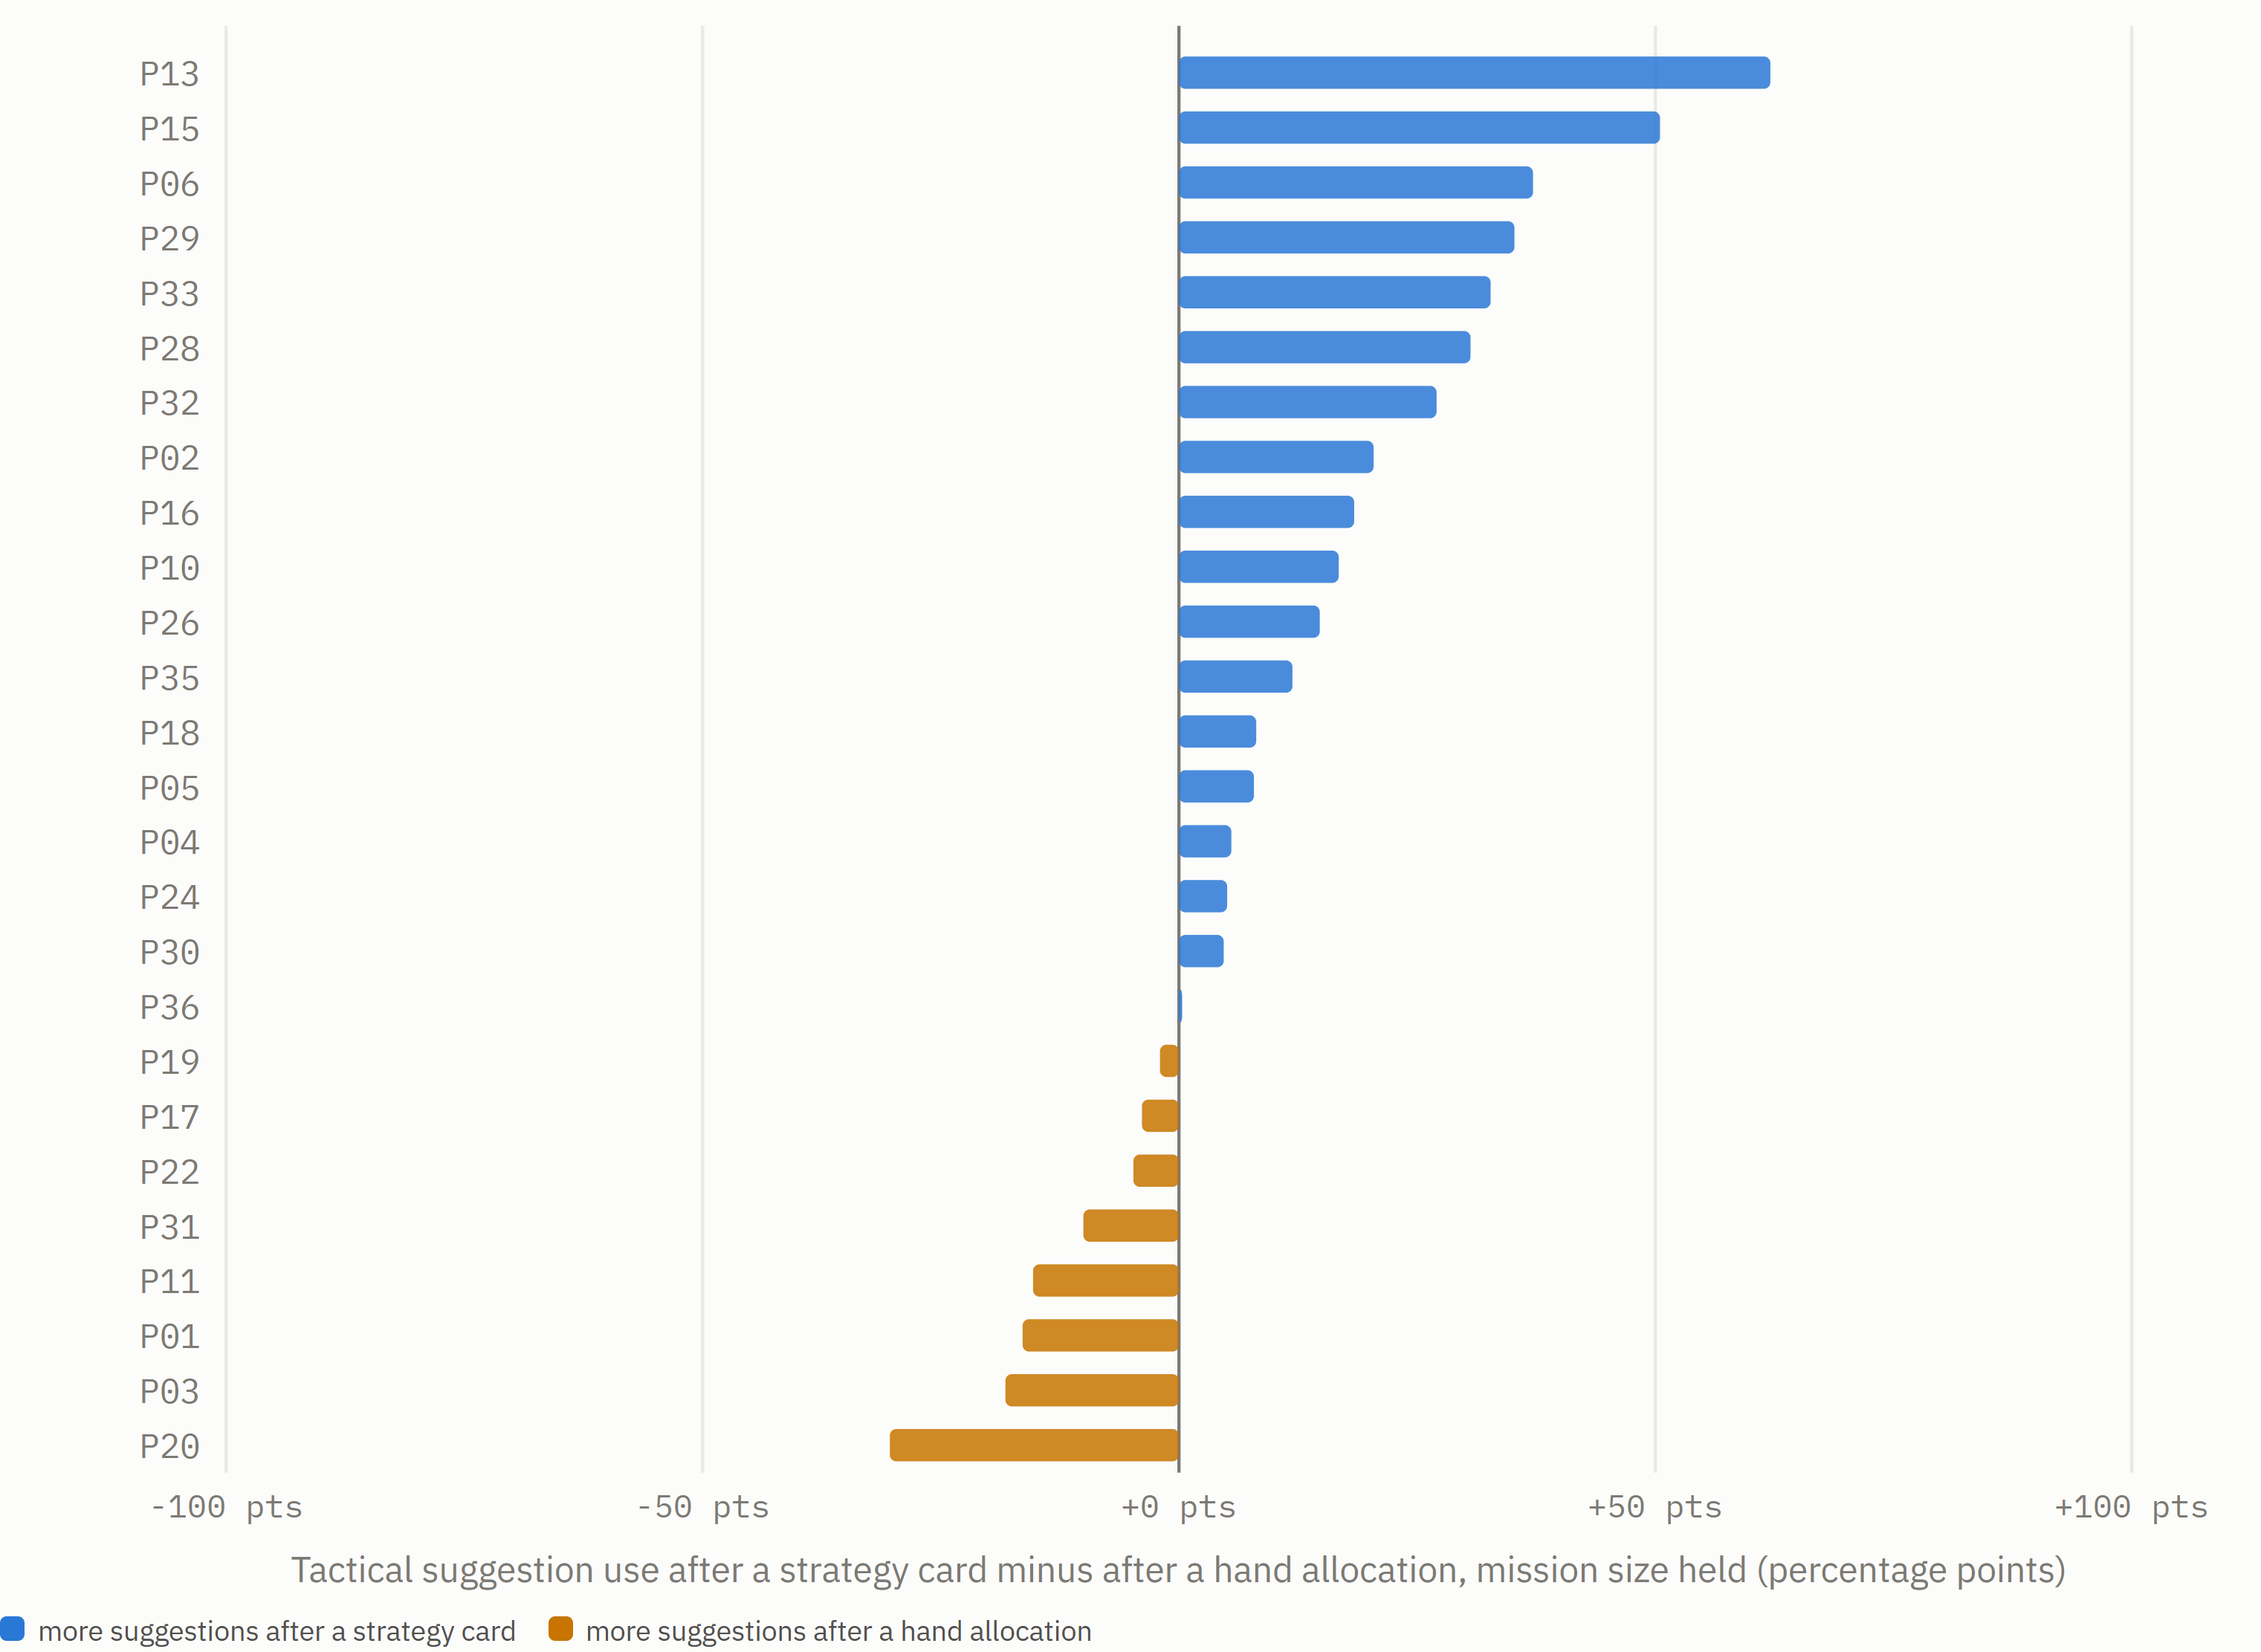
\includegraphics[width=\linewidth,height=0.24\textheight,keepaspectratio]{figs/results/f-size-decides__route-people__gap.png}\par{\scriptsize Other view: Each person's gap, mission size held.}\end{minipage}\hfill
\begin{minipage}[t]{0.49\linewidth}\centering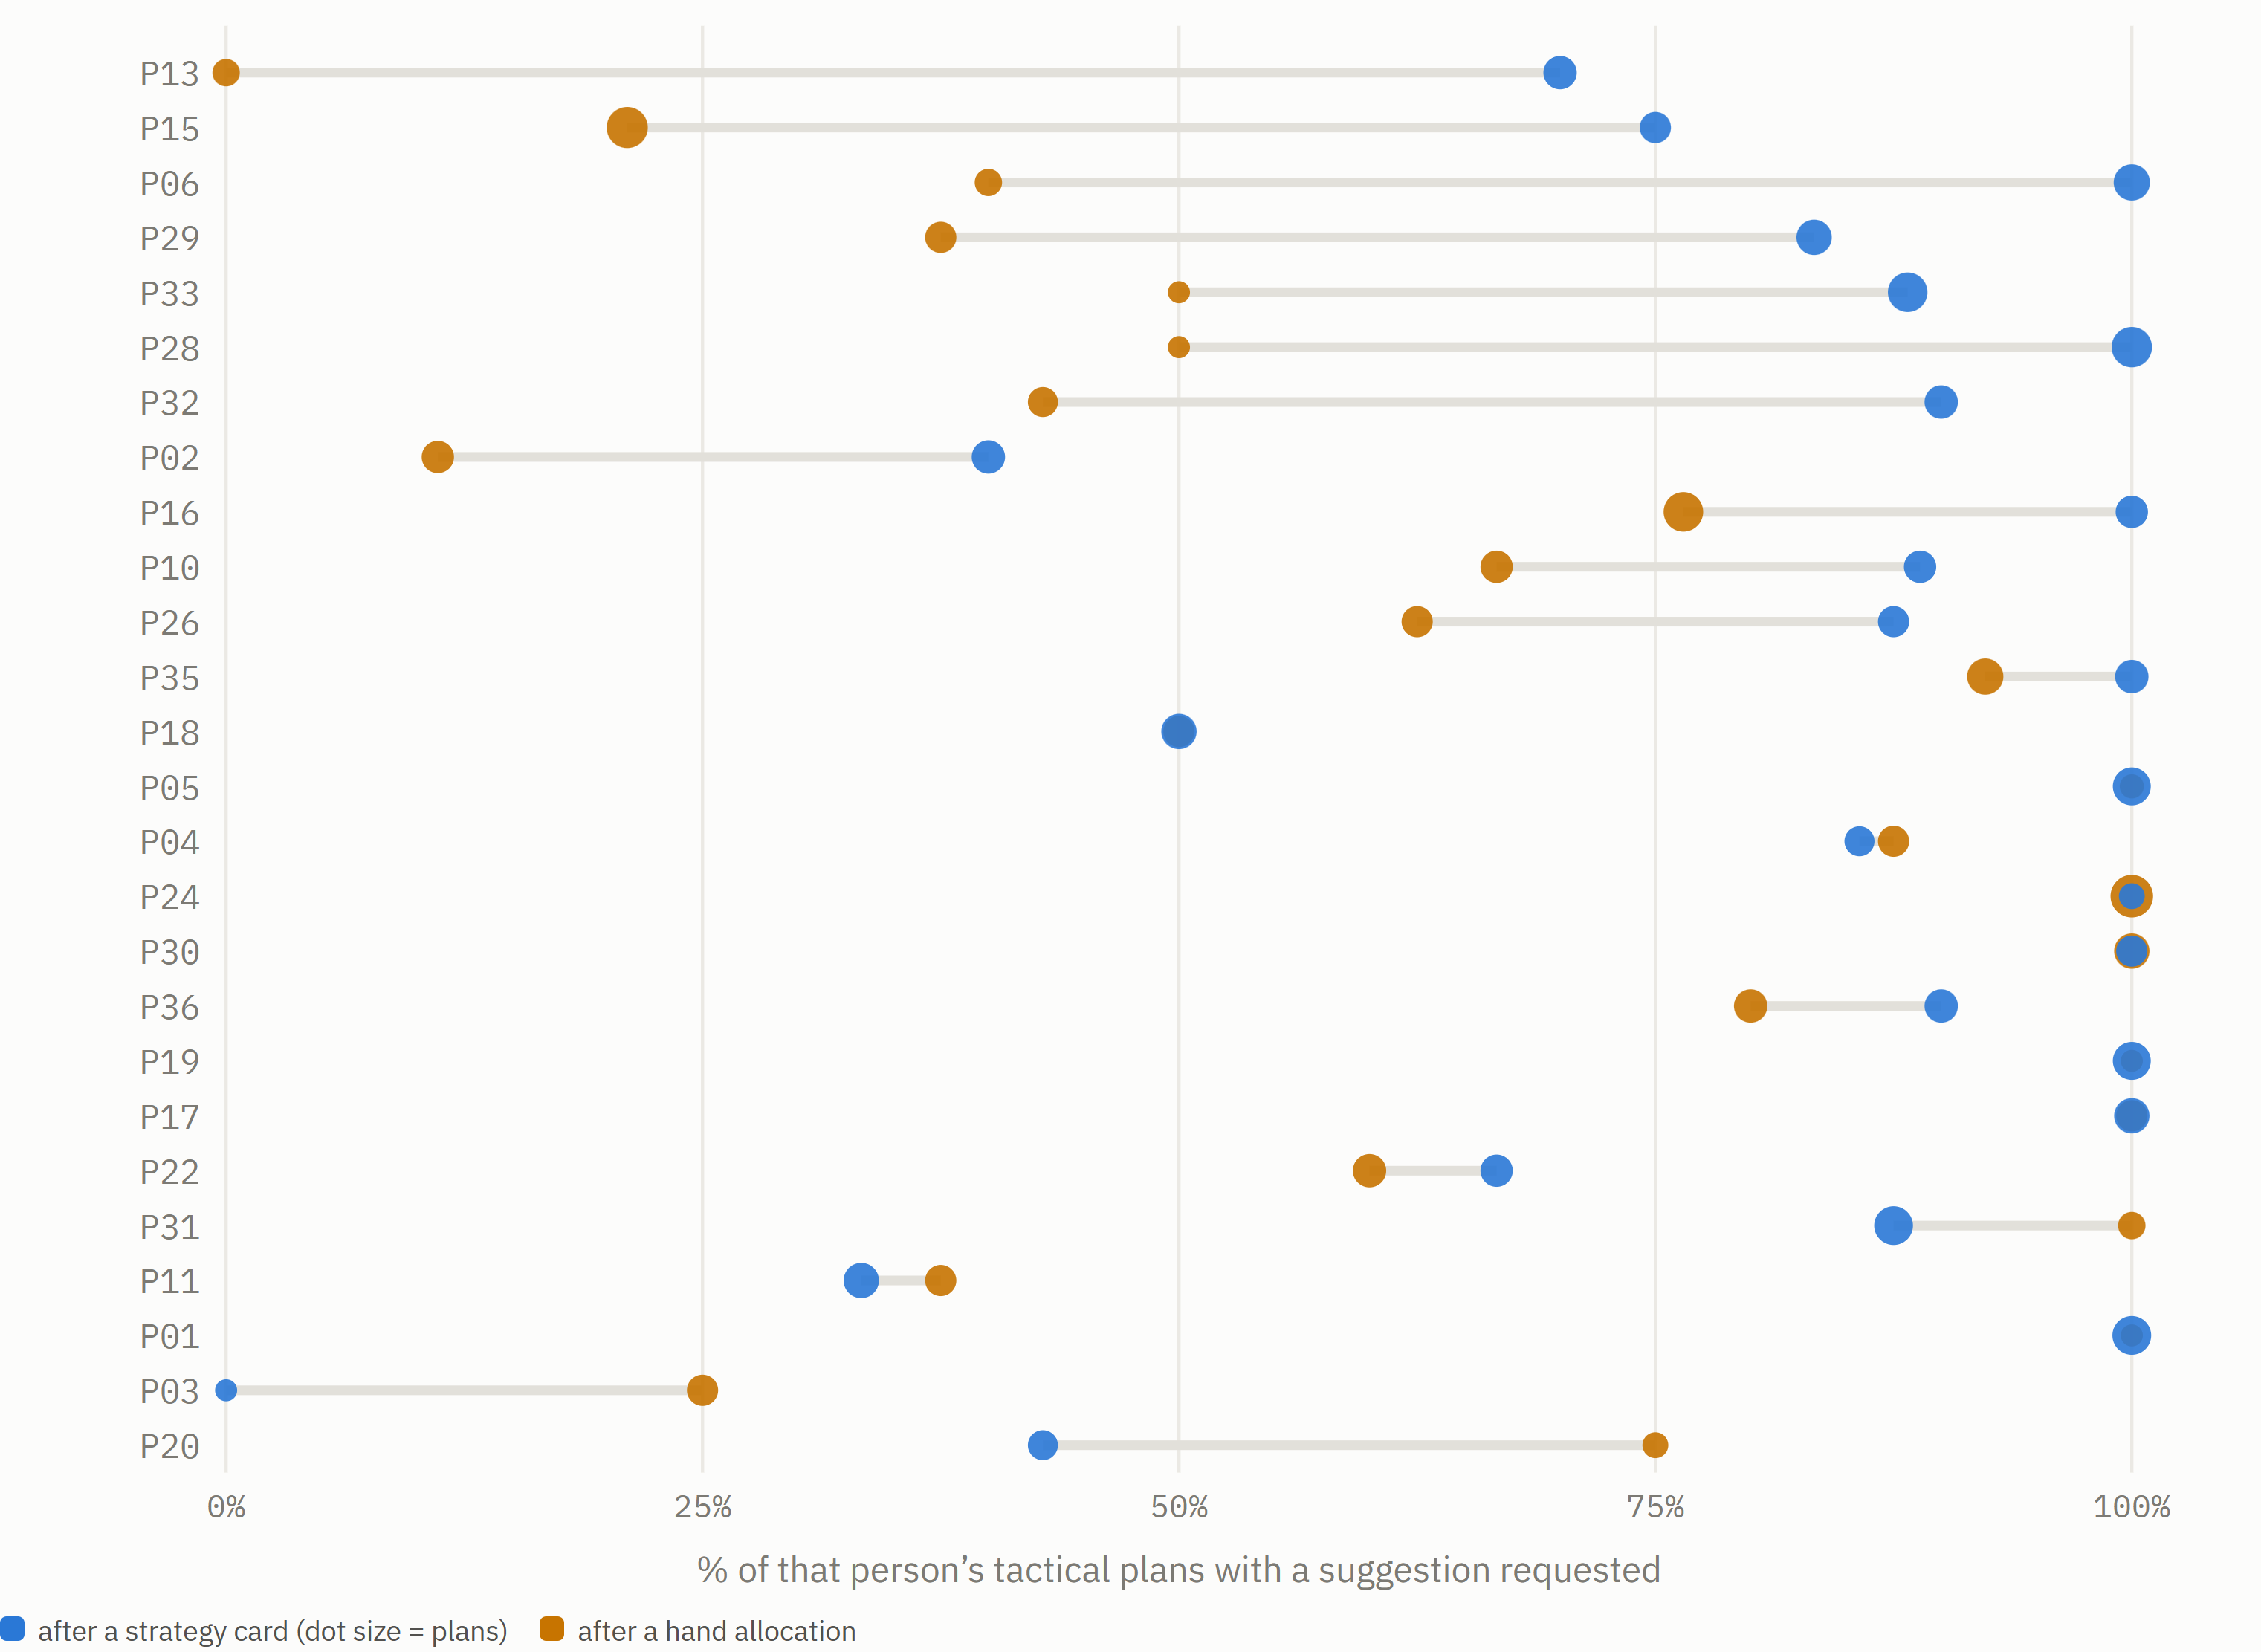
\includegraphics[width=\linewidth,height=0.24\textheight,keepaspectratio]{figs/results/f-size-decides__route-people__rates.png}\par{\scriptsize Other view: Each person's two raw rates.}\end{minipage}

\noindent Key numbers:\begin{itemize}[leftmargin=1.2em,itemsep=0pt]\footnotesize
\item People with $\geq$ 2 plans each way: 26. Gap (size held) positive 17, negative 8, none 1; sign test p = .11; mean gap +11 points.
\item Card vs hand odds ratio, everyone $\times$2.10; leaving out any one person $\times$1.90 (without P15) to $\times$2.40 (without P11), always p < .05.
\item Without the largest gaps: top 1 (P13) $\times$1.97, p = .006; top 3 (P06, P13, P15) $\times$1.63 [1.05, 2.52], p = .03; top 5 $\times$1.46 [0.96, 2.22], p = .08; top 8 $\times$1.23, p = .34.
\item The three largest gaps are 52\% of the summed gap. Not comparable: 6 people almost only planned after a card, 1 almost only after a hand allocation.
\item Also holding fixed whether the mission needs one drone type: $\times$2.13 [1.30, 3.49]; and the number of tasks too: $\times$2.06 [1.24, 3.43], p = .005.
\end{itemize}

\optsec{Why the rule makes sense: the card pays only on big strategic jobs; Suggest is not slower} {\footnotesize [pass 5: extra: may make it in]}

\par\noindent \begin{minipage}[t]{0.49\linewidth}\centering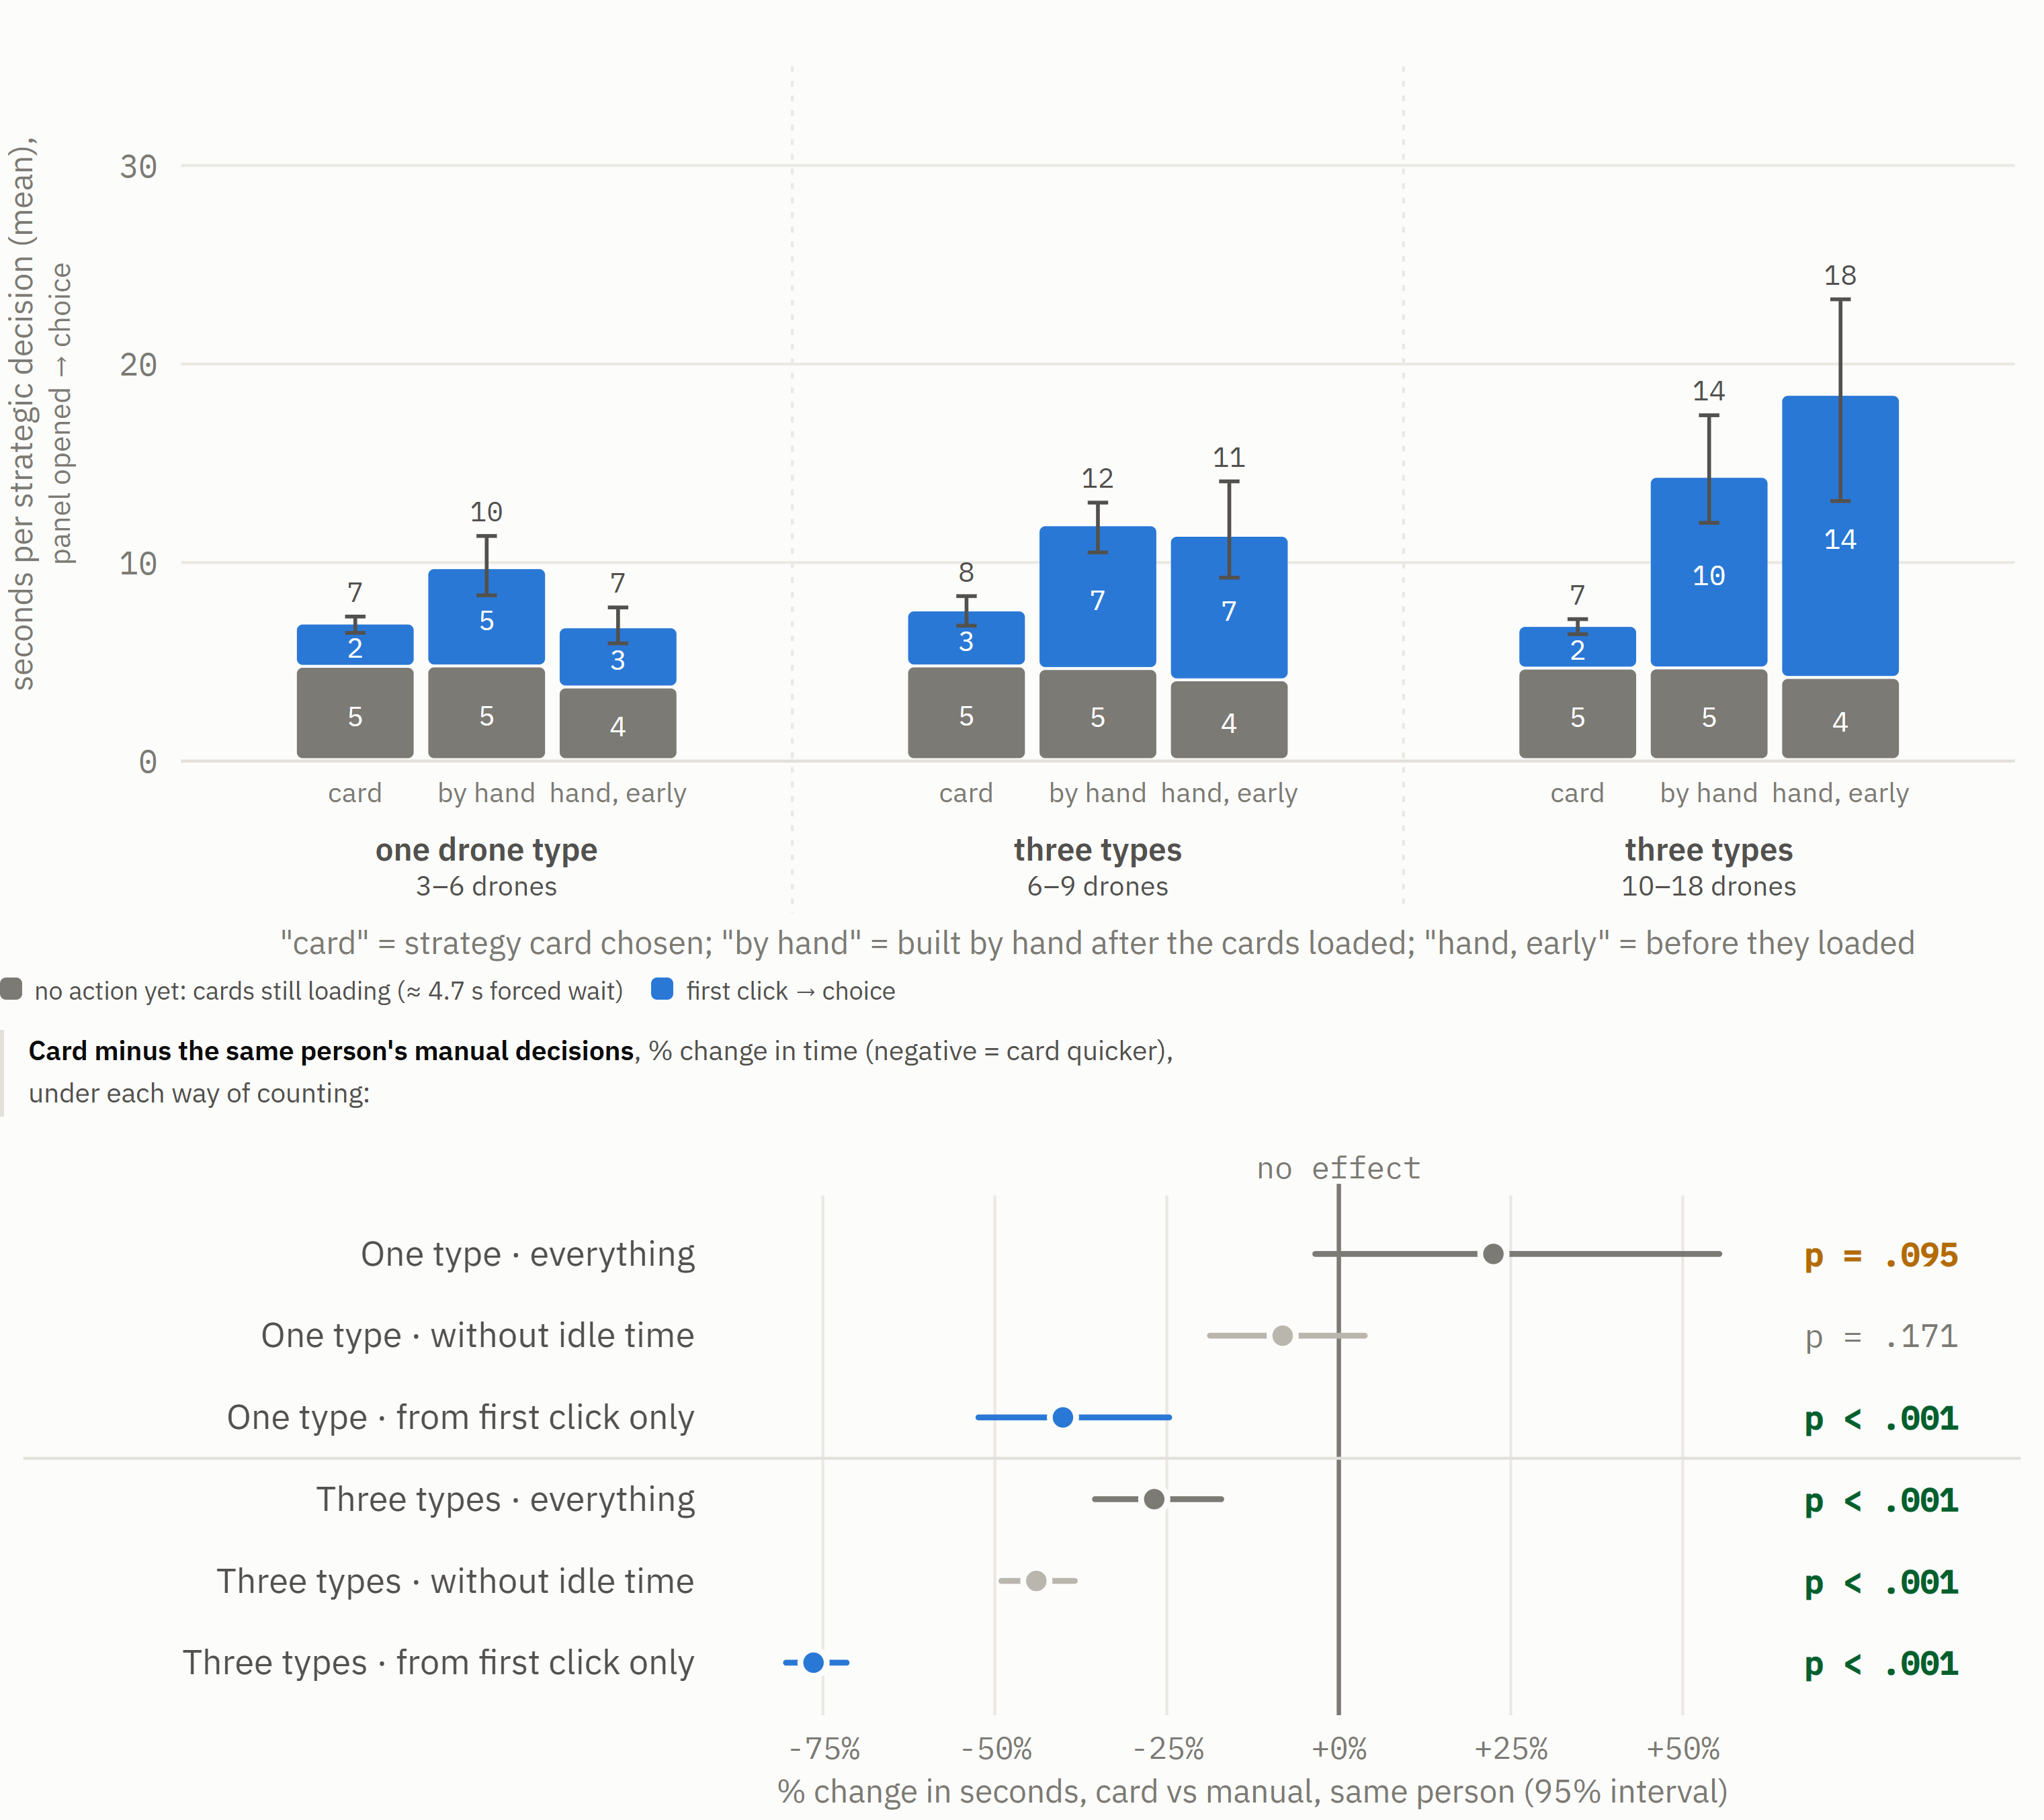
\includegraphics[width=\linewidth,height=0.24\textheight,keepaspectratio]{figs/results/f-size-decides__speed__strat-noidle.png}\par{\scriptsize Other view: Strategic tier, idle time removed.}\end{minipage}\hfill
\begin{minipage}[t]{0.49\linewidth}\centering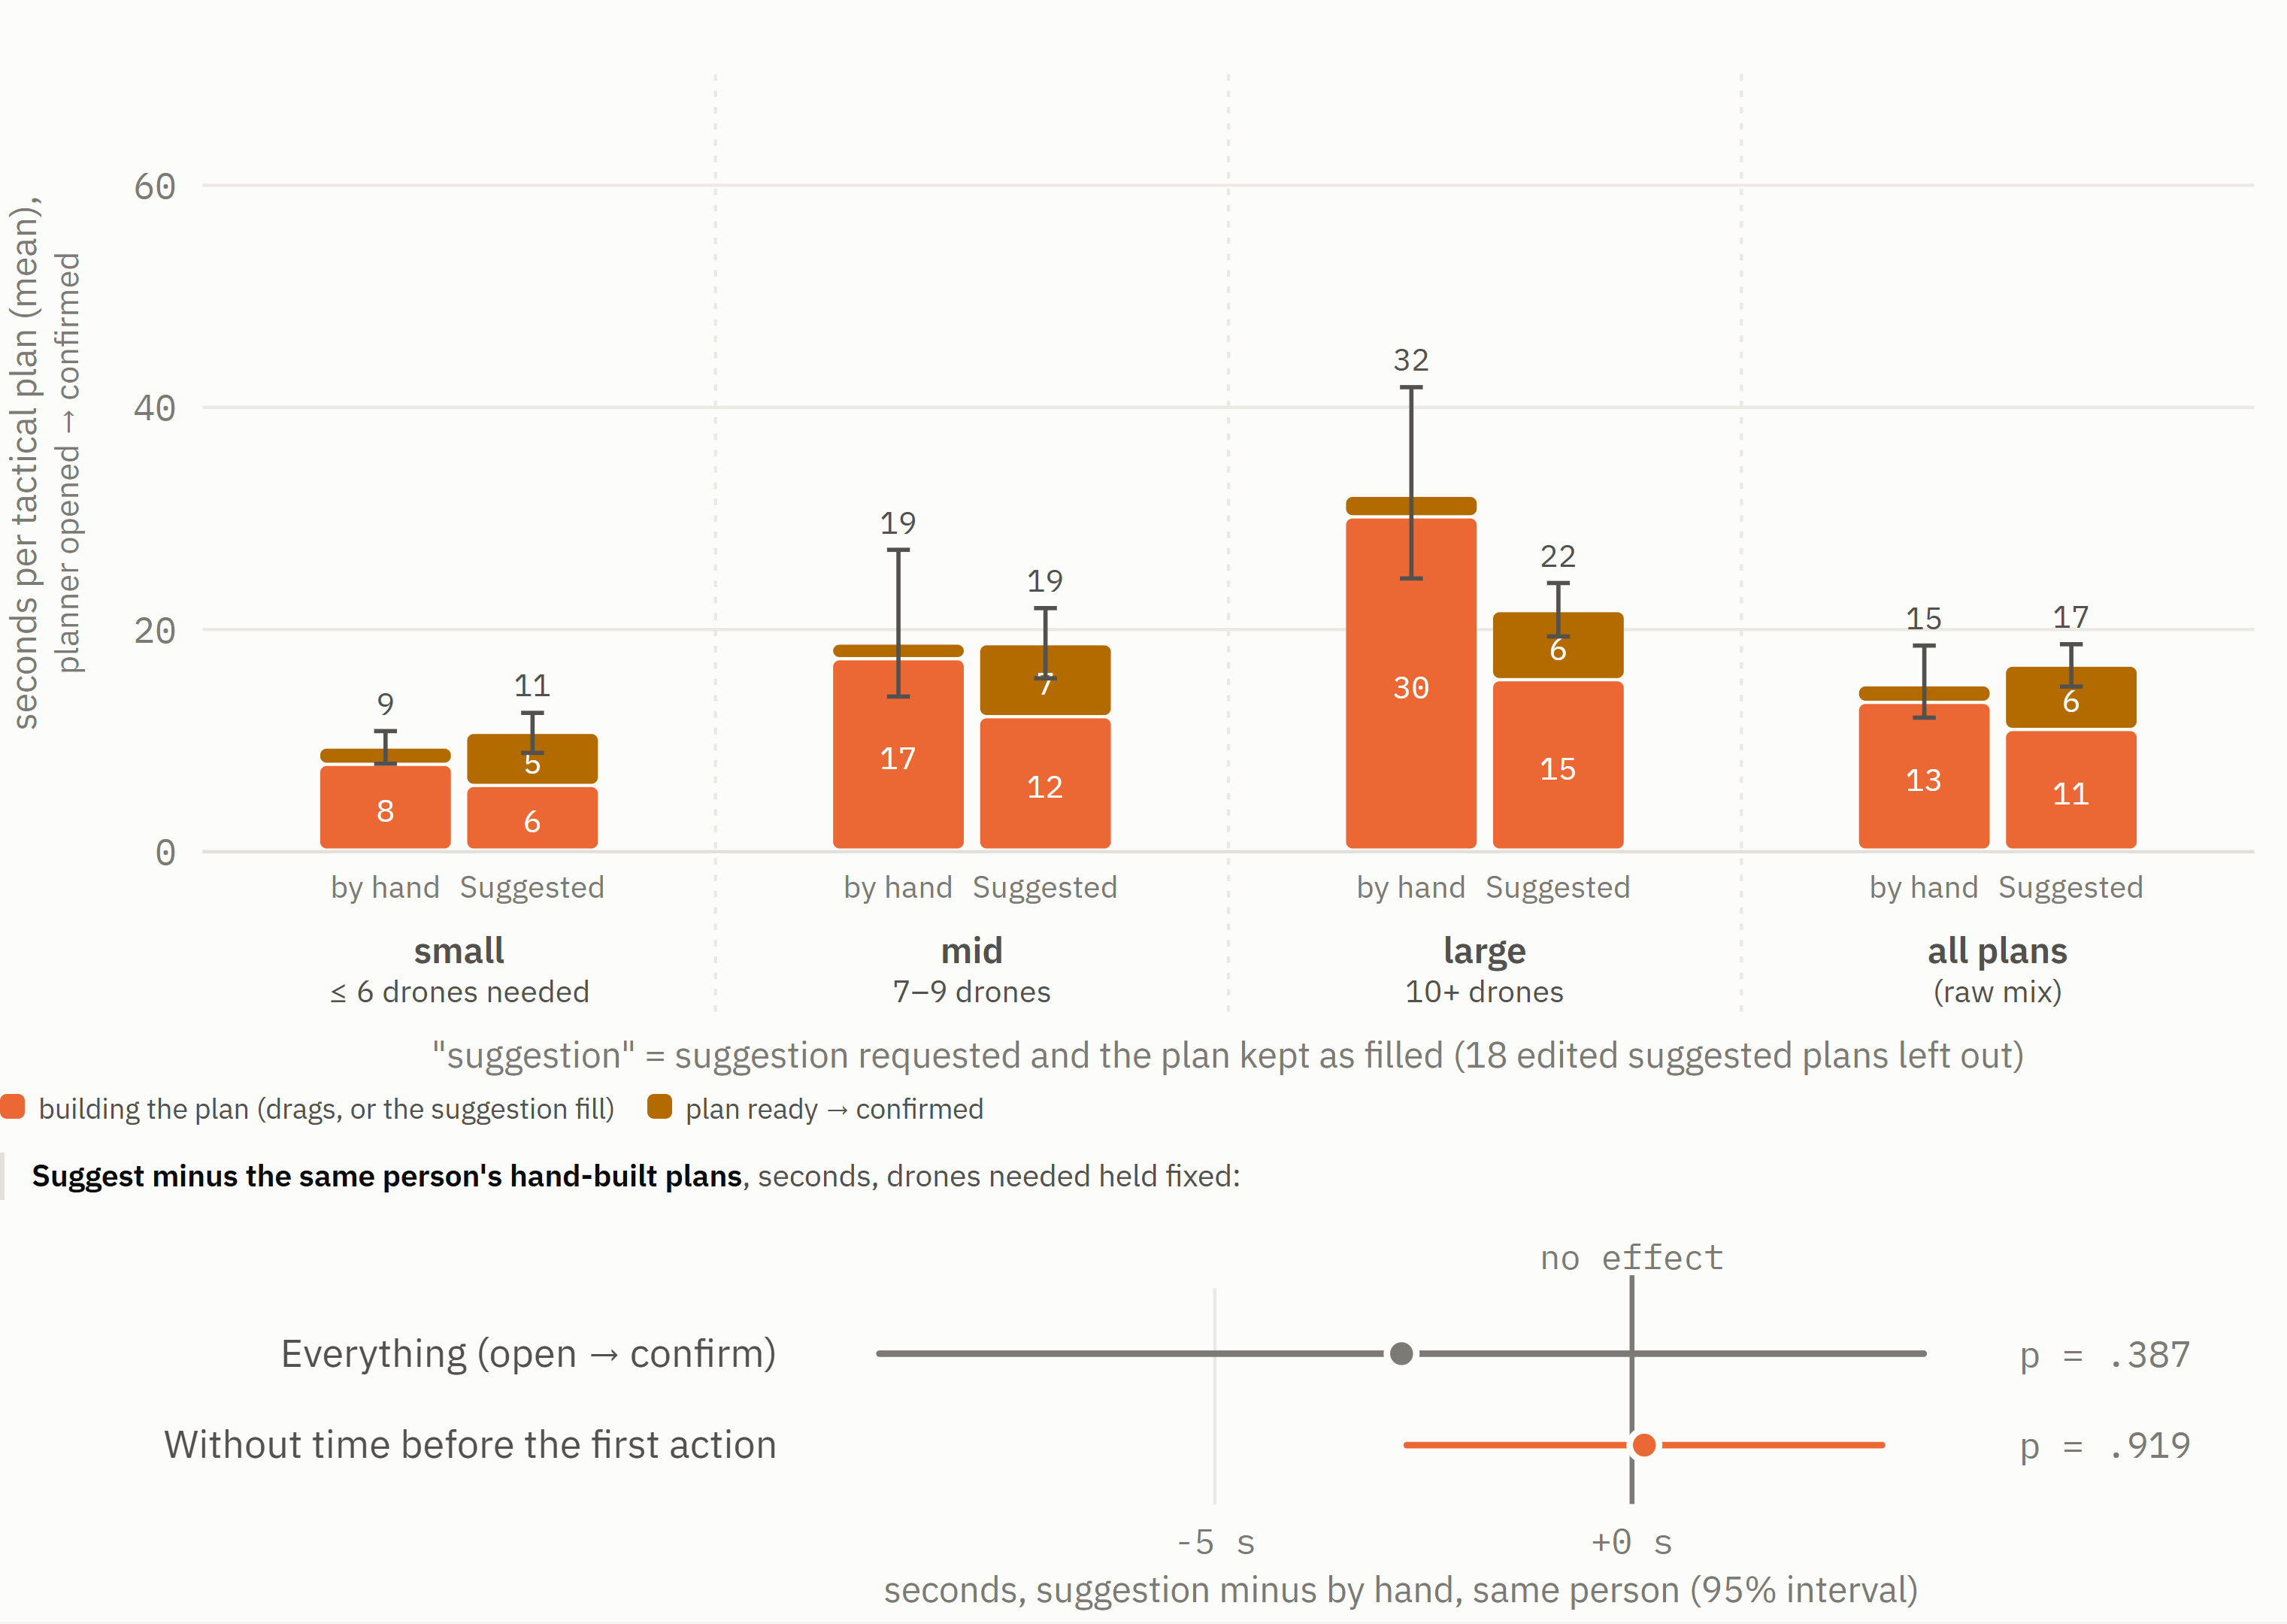
\includegraphics[width=\linewidth,height=0.24\textheight,keepaspectratio]{figs/results/f-size-decides__speed__tac-noidle.png}\par{\scriptsize Other view: Tactical tier, idle time removed.}\end{minipage}

\noindent Key numbers:\begin{itemize}[leftmargin=1.2em,itemsep=0pt]\footnotesize
\item Strategic, card vs manual, same person, \% change in time: everything: one-type +22\% [$-$3, +55], p = .09; three-type $-$27\% [$-$35, $-$17], p < .001
\item Without idle time: one-type $-$8\% [$-$19, +4], p = .17; three-type $-$44\% [$-$49, $-$38], p < .001. From the first click only: one-type $-$40\%, three-type $-$76\% (both p < .001)
\item Strategic means (s), loading + idle + acting: one-type card 4.7 + 6.5 + 2.2 = 13.3; by hand after cards 4.7 + 8.6 + 5.0 = 18.2; before cards 3.7 + 0.7 + 3.0 = 7.4. Three-type 10--18 drones: card 4.6 + 7.3 + 2.1 = 14.0; by hand 4.6 + 10.1 + 9.7 = 24.4
\item Tactical means (s), idle + building + ready $\rightarrow$ confirmed: all plans by hand 14.2 + 13.3 + 1.6 = 29.1 (144) vs Suggest 10.6 + 10.9 + 5.8 = 27.2 (465); large missions 17.9 + 30.0 + 1.9 = 49.8 (22) vs 10.0 + 15.3 + 6.2 = 31.5 (159)
\item Tactical, Suggest minus by hand, same person, drones needed held: everything $-$2.8 s [$-$9.0, +3.5], p = .39; without idle time +0.2 s [$-$2.7, +3.0], p = .92; Suggest $\times$ size (without idle) $-$1.3 s per doubling, p = .47
\item Tactical plans idle for more than 10 s: 54\% had another mission's strategic panel opened before the first action (176 plans); all plans 22\%
\end{itemize}

\noindent Highlighted quotes not used above:\begin{quotelist}
\item ``I think the key strength when I [am] using the agent is it can help me to save the time and energy to those specific deployments''\,---\,P28 (debrief 0:32:10)
\item ``the point is, it takes me so much time to untangle that, that maybe it probably will not be faster if I do it myself manually. So as long as the AI makes sure that everything is covered once.''\,---\,P17 (think-aloud s1 0:07:07)
\item ``Manually, [I] can't wait for the processing, to be honest.''\,---\,P21 (think-aloud s1 0:09:32)
\item ``I think even if the tactical agent gave me a dodgy suggestion and the mission failed and I lost points, I probably would have gained more points from the time saved...''\,---\,P11 (debrief 0:30:11)
\item ``I think I was definitely a bit slower than the, than the algorithm there.''\,---\,P22 (think-aloud s1 0:07:11)
\item ``You know, it's quicker to get a suggestion, but it is less clicking, and it seems to do what I would do.''\,---\,P32 (think-aloud s1 0:10:07)
\item ``So, it just seems quicker to just send some myself than wait for the recommendation. I might just be impatient.''\,---\,P32 (think-aloud s1 0:03:09)
\item ``So, when we are trying to do with the tactical screen, I find the agent is quite slow.''\,---\,P27 (debrief 0:29:10)
\item ``Yeah, when I located, I think sometimes the AI will take a little longer. And I just mess up my strategy''\,---\,P26 (debrief 0:28:37)
\end{quotelist}

\optsec{Where the tactical time goes: hand-built and Suggest plans are close, with a small edge to Suggest in carrying the plan out} {\footnotesize [pass 5: for the paper]}

\par\noindent \begin{minipage}[t]{0.49\linewidth}\centering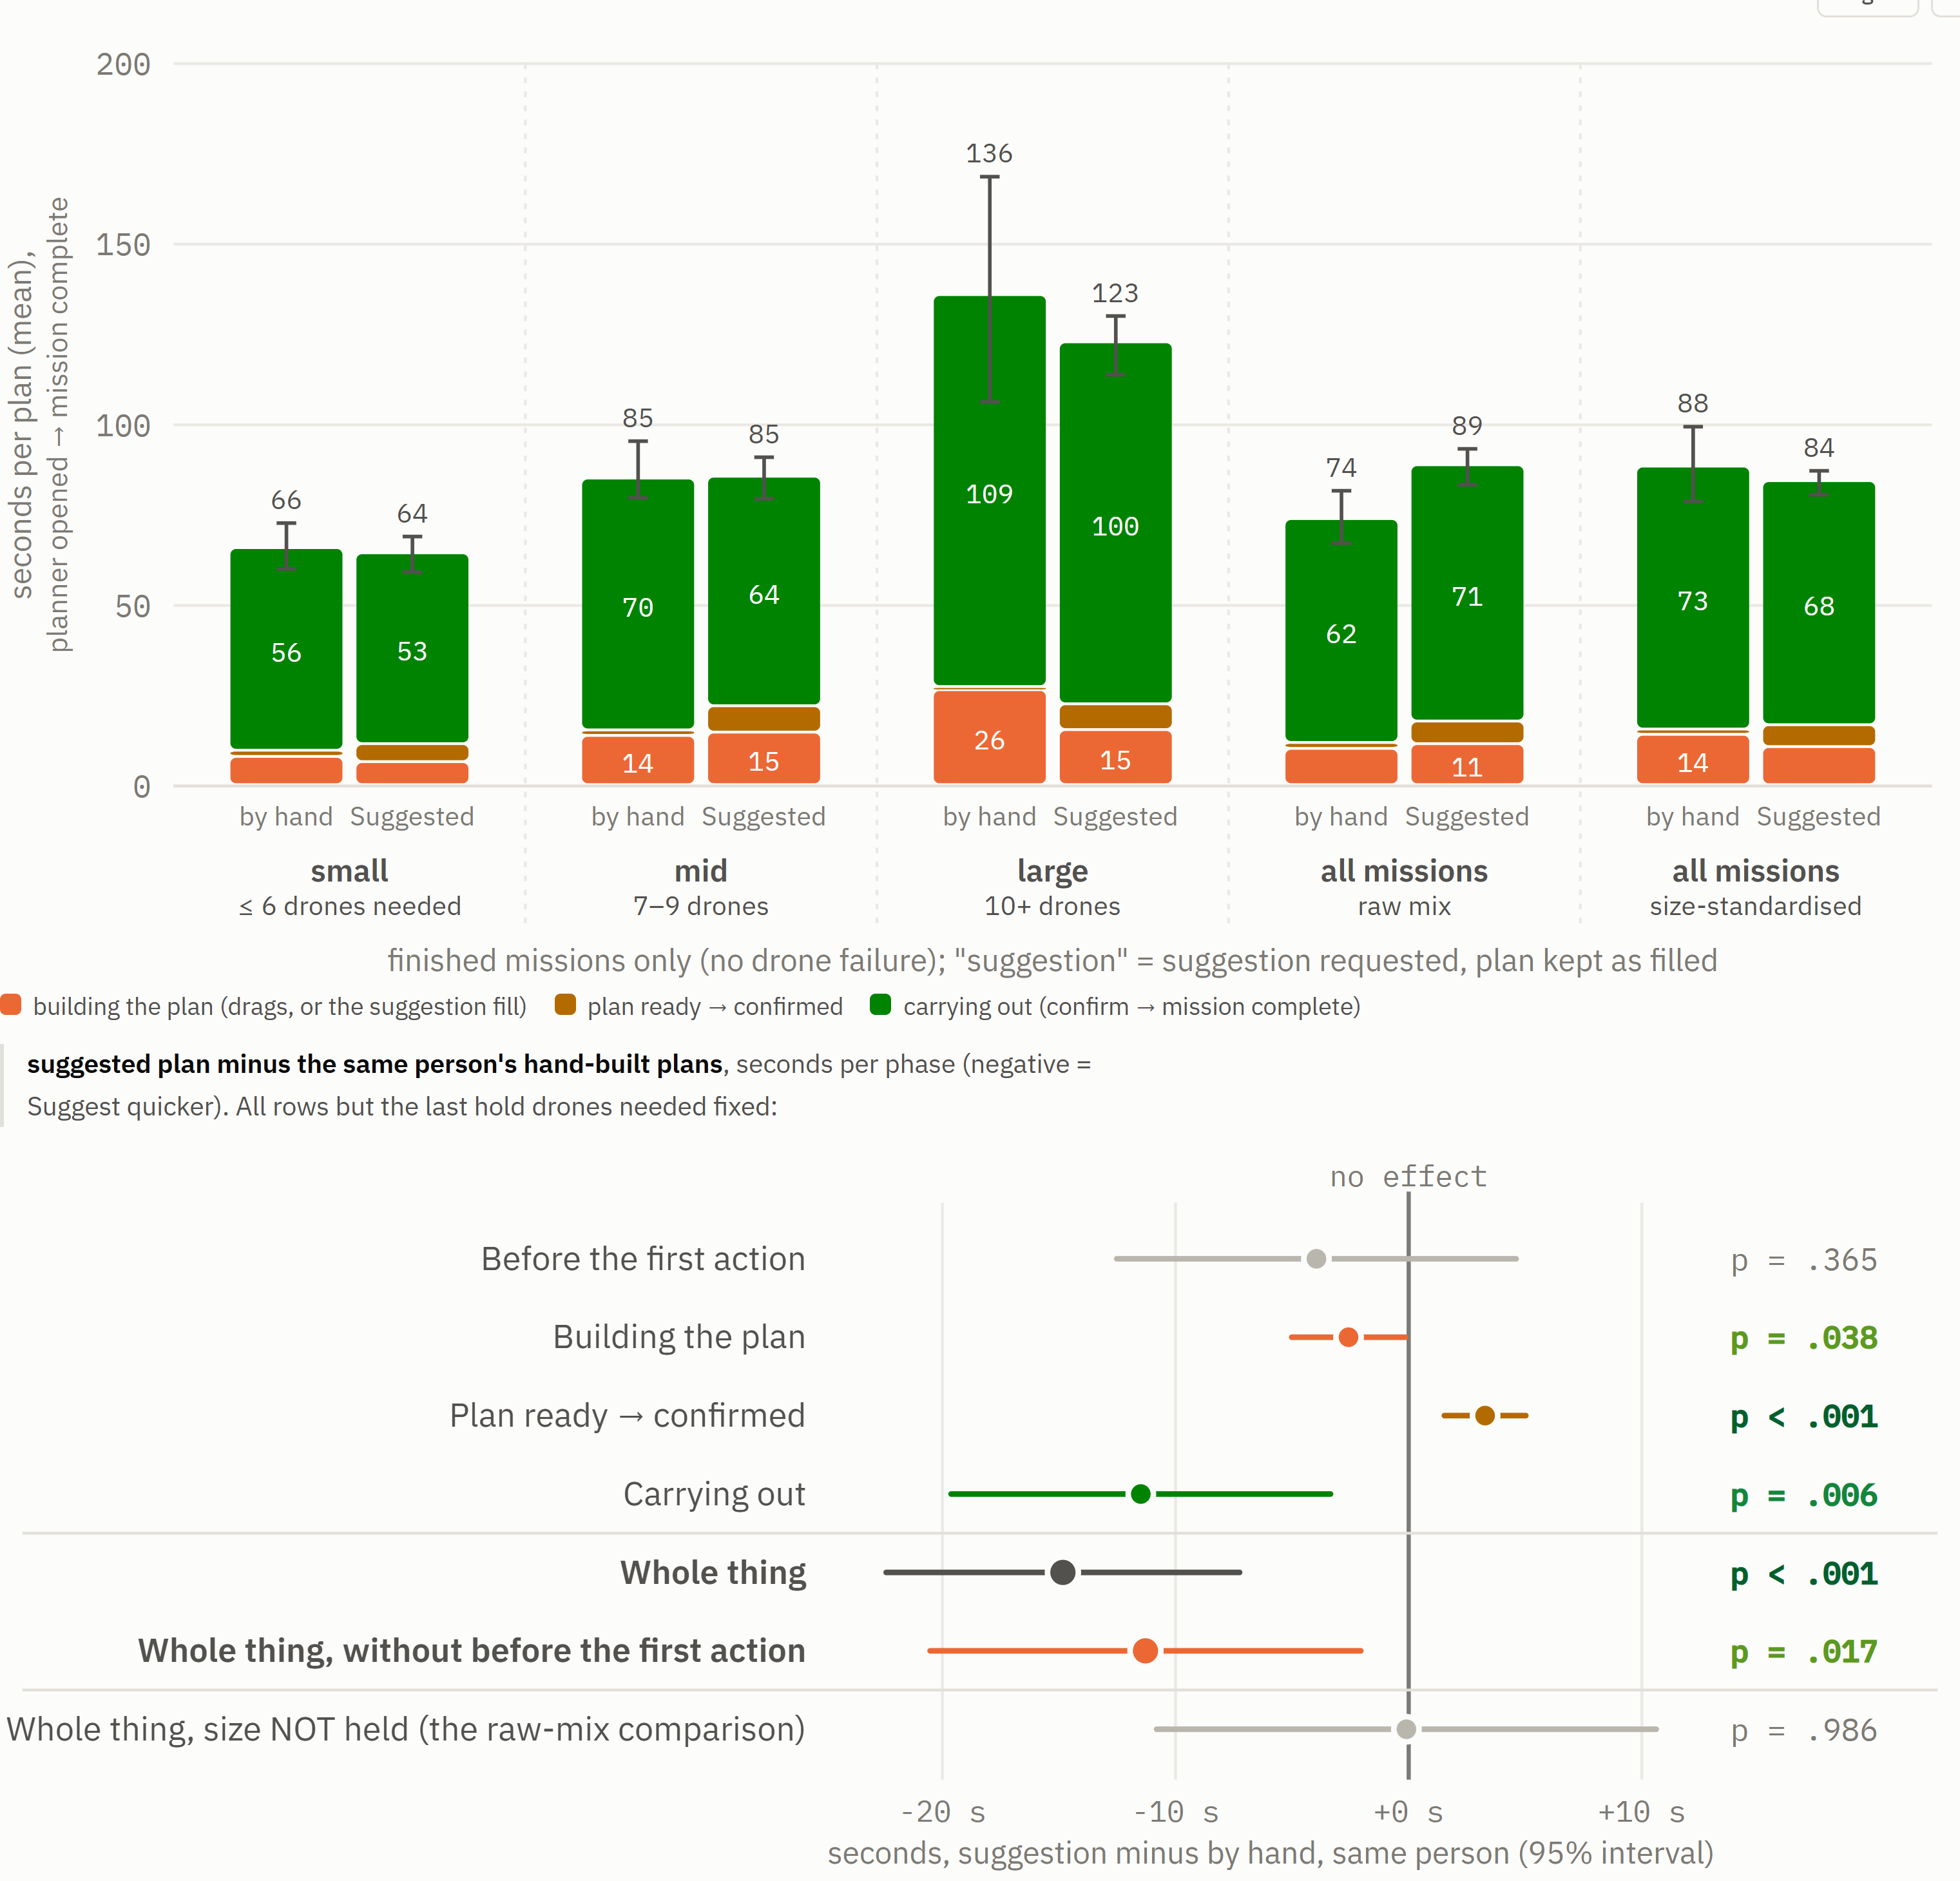
\includegraphics[width=\linewidth,height=0.24\textheight,keepaspectratio]{figs/results/f-size-decides__parallel__noidle.png}\par{\scriptsize Other view: Without the time before the first action.}\end{minipage}

\noindent Key numbers:\begin{itemize}[leftmargin=1.2em,itemsep=0pt]\footnotesize
\item Suggest minus hand-built, same person, drones needed held (315 finished plans): before the first action $-$4.0 s [$-$12.5, +4.6], p = .37; building $-$2.6 s [$-$5.0, $-$0.1], p = .038; ready $\rightarrow$ confirmed +3.3 s [+1.5, +5.0], p < .001; carrying out $-$11.5 s [$-$19.6, $-$3.4], p = .006; whole $-$14.8 s [$-$22.4, $-$7.3], p < .001
\item Whole thing without the time before the first action: $-$11.3 s [$-$20.5, $-$2.1], p = .017; whole thing with size not held: $-$0.1 s [$-$10.8, +10.6], p = .99
\item Means (s), hand vs kept Suggest: small 78.5 vs 74.8 (63 vs 97 plans); mid 113.6 vs 102.0 (12 vs 59); large 166.6 vs 131.6 (6 vs 75); all, raw 90.2 vs 100.2; all, size-standardised 109.3 [102.7, 119.4] vs 95.7 [91.9, 99.1]
\item Size mix of finished plans: hand-built 78\% small, 15\% mid, 7\% large (mean 5.7 drones needed); Suggest 42\%, 26\%, 32\% (mean 8.8)
\item All 627 plans, first three phases: before $-$2.9 s, p = .29; building $-$3.2 s [$-$6.2, $-$0.1], p = .04; ready $\rightarrow$ confirmed +3.3 s [+2.0, +4.6], p < .001
\item Carrying out, including missions with a drone failure (378): $-$8.1 s [$-$17.1, +0.9], p = .08: same direction, less certain
\item Projected completion vs the assistant's own plan at open, median: hand-built +10.3 s [3.7, 28.3] (144 plans), kept Suggest +1.6 s [0.8, 4.0] (468), edited Suggest +38.7 s (18)
\item Interleaving, round-1 specification re-run: odds $\times$4.83 [2.24, 10.40], p < .001 (630 plans, 33 people); raw 45\% vs 19\%; 28\% vs 11\% actually allocated another mission
\item Operator time, building + ready $\rightarrow$ confirmed, Suggest minus hand-built, same person, size held: $-$2.6 s + 3.3 s $\approx$ +0.7 s (negligible)
\item From the retired ``who does better'' finding: within a person, card missions vs own manual missions, completed in full odds $\times$0.81 [0.55, 1.18], p = .27 (raw 60\% vs 62\%); session score per +25 points of strategy card choice $-$0.10 SD [$-$0.47, 0.27], p = .61. Between people, heavier card users complete more ($\times$1.32 per 25 points, p = .004): the difference is in the people, not the advice
\end{itemize}

\optsec{What operators say} {\footnotesize [pass 5: for the paper]}

\noindent Key numbers:\begin{itemize}[leftmargin=1.2em,itemsep=0pt]\footnotesize
\item C03 10 of 33; C04 15 of 33; C05 8 of 33
\item C03 vs others, size slope ratio: strategic $\times$1.28 [0.69, 2.38], p = .43; tactical $\times$1.43 [0.93, 2.20], p = .10
\end{itemize}
\end{options}

\clearpage

% ======== f-manual-cards ========

\subsection{Hand-built allocations are anchored on the strategy cards}\label{sec:res:manual-cards}

When operators allocated by hand after seeing the strategy cards, their numbers tracked the cards: one more drone on the Conservative card meant about half a drone more in the hand-built allocation, beyond what the mission needed. Operators who decided before the cards appeared showed no such link, which makes this anchoring rather than both following the mission. Hand-built allocations mostly sat at or below the cards (44\% below both, 33\% equal to one, 14\% between and 8\% above).

% --- f-manual-cards#dots (pass 5: for the paper) ---

\phantomsection\label{sec:res:manual-cards:dots}
Figure~\ref{fig:res:manual-cards:dots} shows every hand-built allocation (209) against the Conservative card. Counting all drone types, allocations on small one-type missions sit about one drone below the card; counting only the types the mission needs, they match it ($+0.05$ drones). The apparent trimming of small missions is almost entirely the card's spare drones of unneeded types being left off. On big three-type missions hand-built allocations sit about one drone above the card. When short of drones, some sent everything they had: ``All right. Let's just send everything I have. Edit, give me five red ones. Five green ones. Hit it.'' (P10).

\begin{figure}[H]
\centering
\begin{subfigure}[t]{\linewidth}
\centering
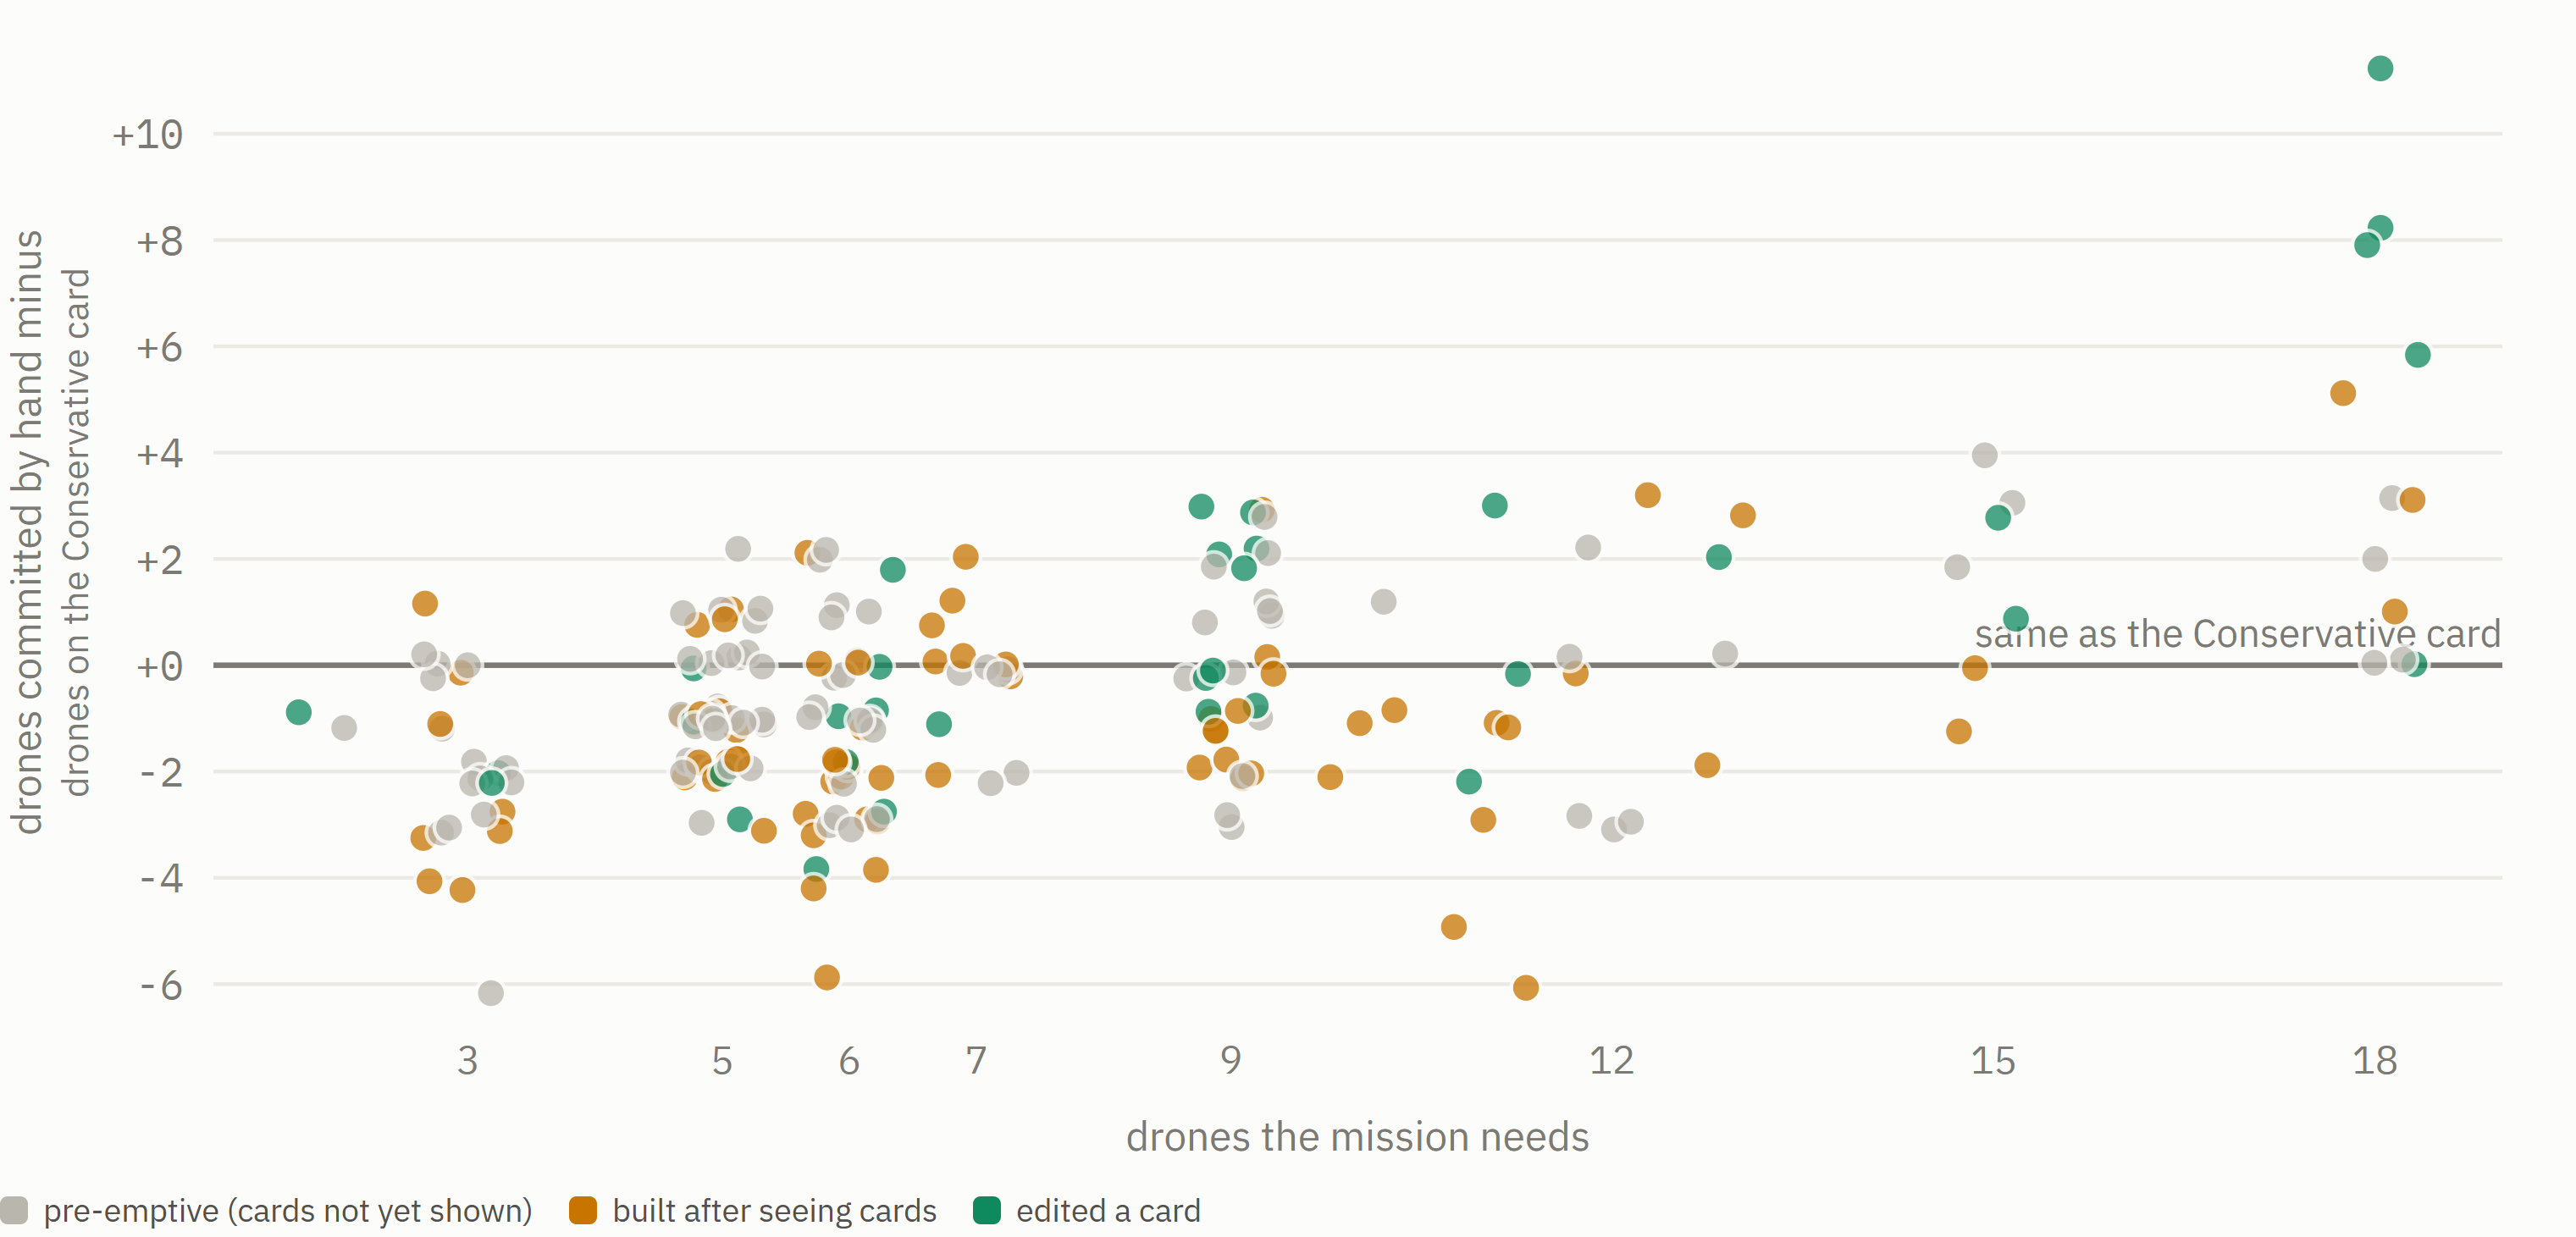
\includegraphics[width=\linewidth,height=0.21\textheight,keepaspectratio]{figs/results/f-manual-cards__dots__all.png}
\caption{All drone types.}
\label{fig:res:manual-cards:dots:all}
\end{subfigure}
\par\smallskip
\begin{subfigure}[t]{\linewidth}
\centering
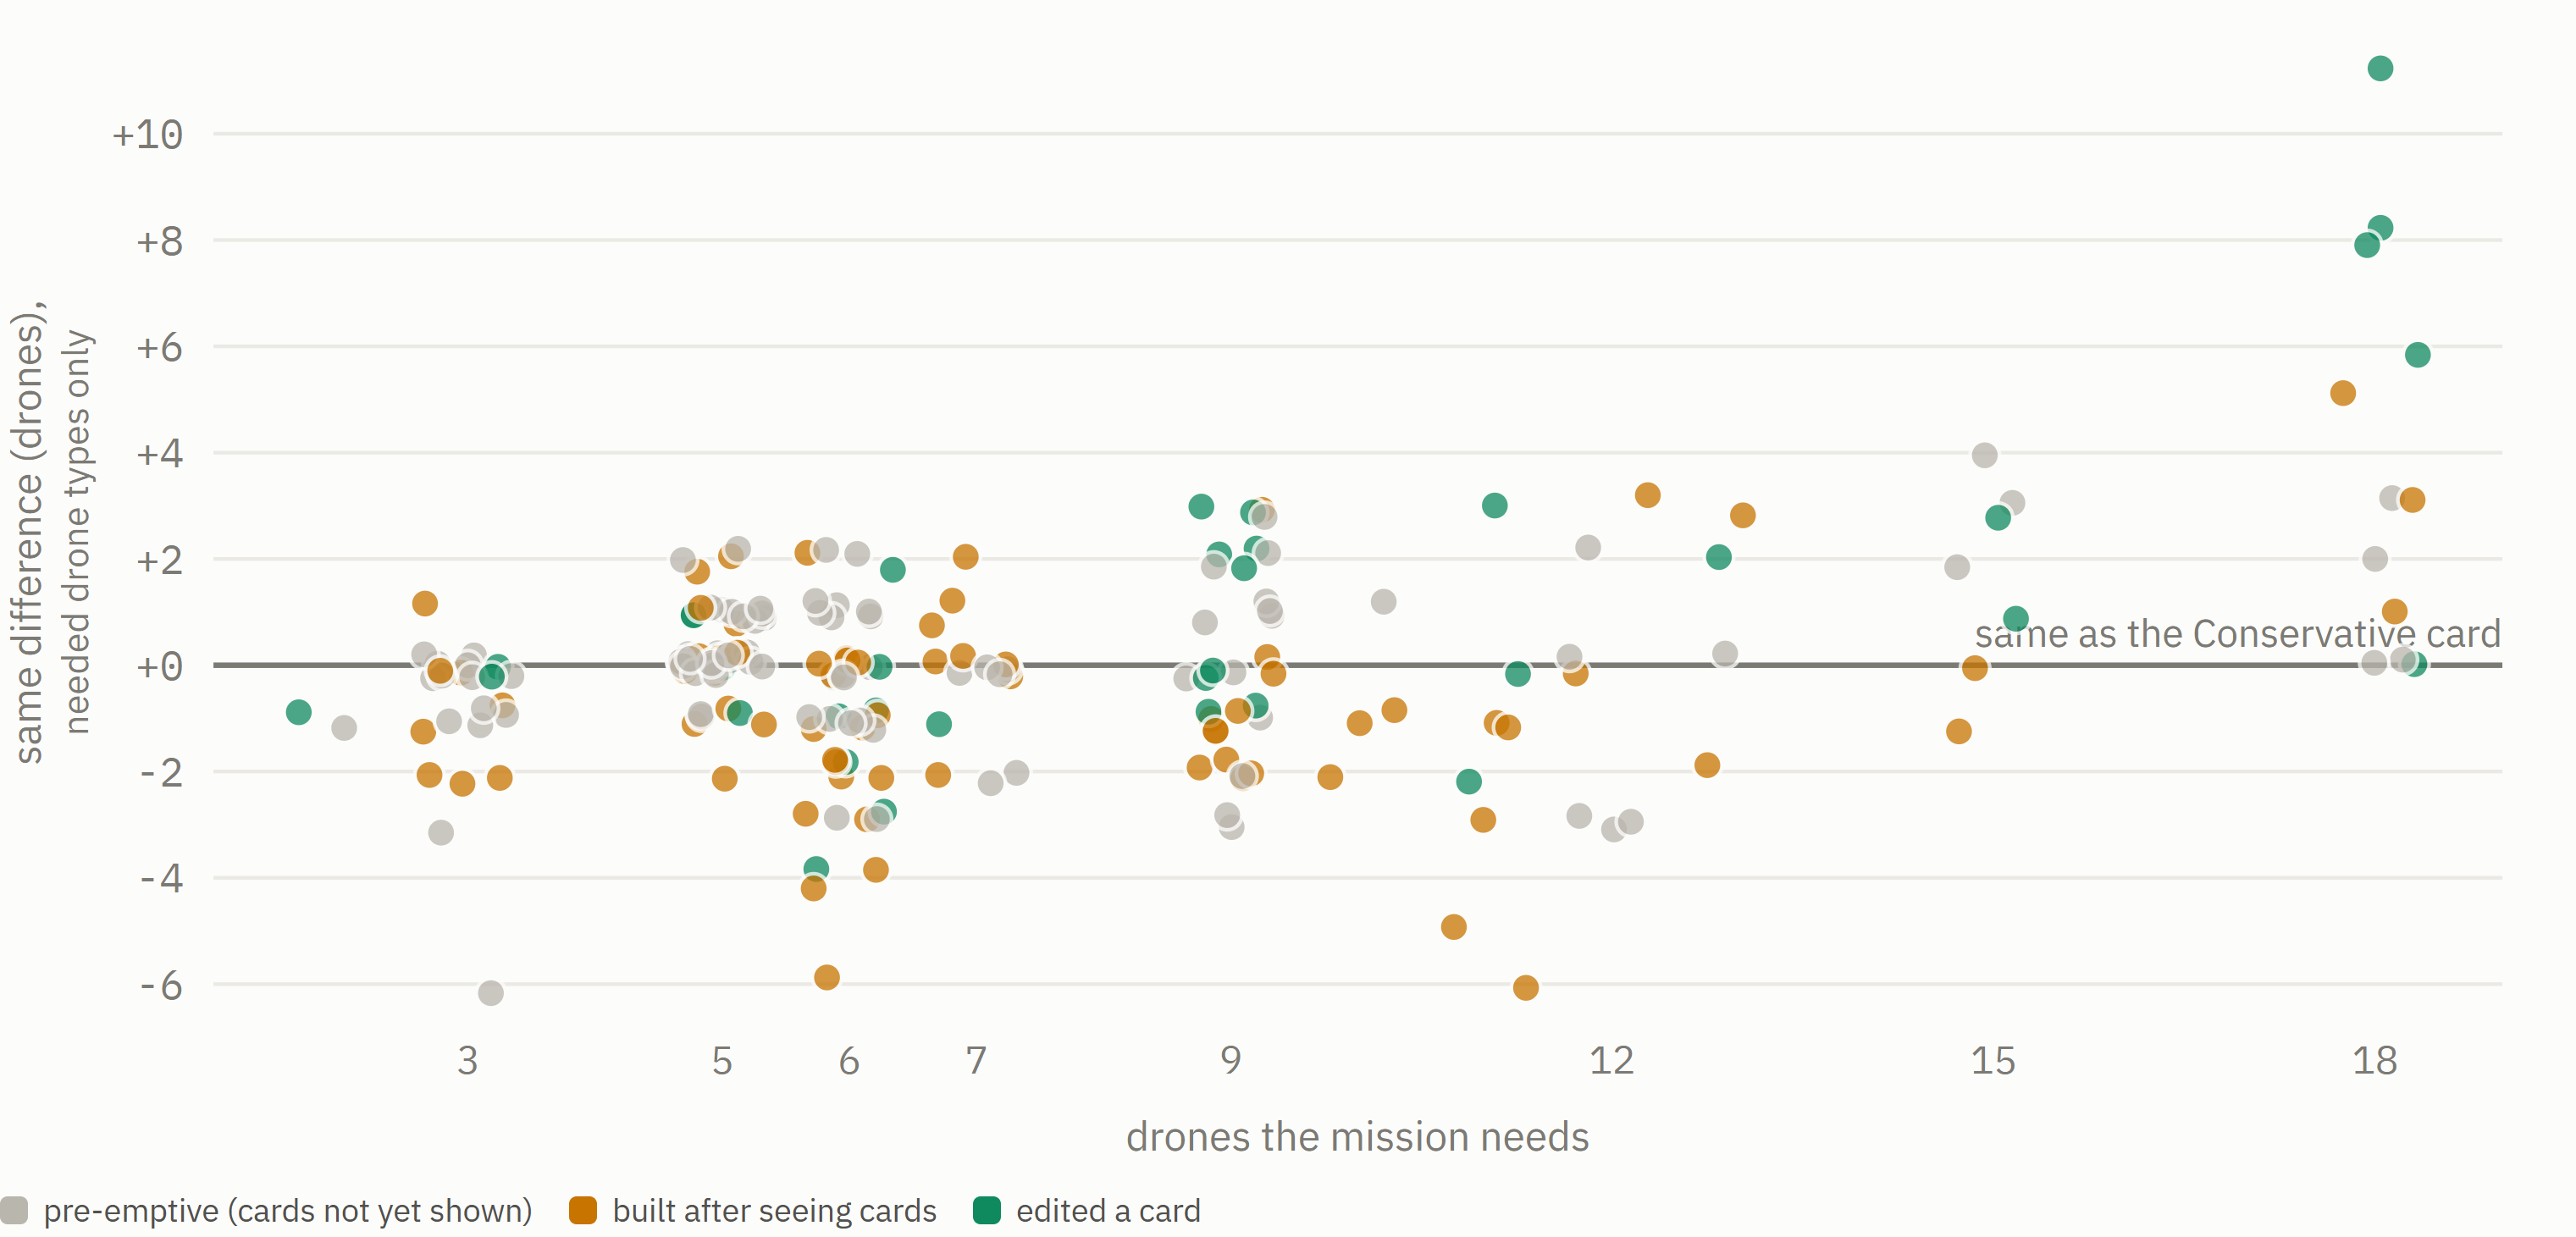
\includegraphics[width=\linewidth,height=0.21\textheight,keepaspectratio]{figs/results/f-manual-cards__dots__needed.png}
\caption{Needed drone types only.}
\label{fig:res:manual-cards:dots:needed}
\end{subfigure}
\par\smallskip
\caption{\textbf{The trim on small missions is the card's unneeded spare.} Drones committed by hand minus drones on the Conservative card, by the drones the mission needs: (a) all drone types, (b) needed types only.}
\label{fig:res:manual-cards:dots}
\end{figure}

% --- f-manual-cards#position (pass 5: for the paper) ---

\phantomsection\label{sec:res:manual-cards:position}\label{sec:res:manual-cards:said}
Allocations built before the cards appeared landed exactly on a card total more often than those built after seeing them (39\% against 27\%, Figure~\ref{fig:res:manual-cards:position:raw}), so matching a card is partly just the obvious allocation rather than copying; balanced for the mission, the difference is too small to tell apart (37\% against 29\%). Some wanted something the two cards did not offer: ``But whenever I clicked manual, it's either been for the cause of `they are sending too much', or I want it to be somewhere between those two levels'' (P17).

\begin{figure}[H]
\centering
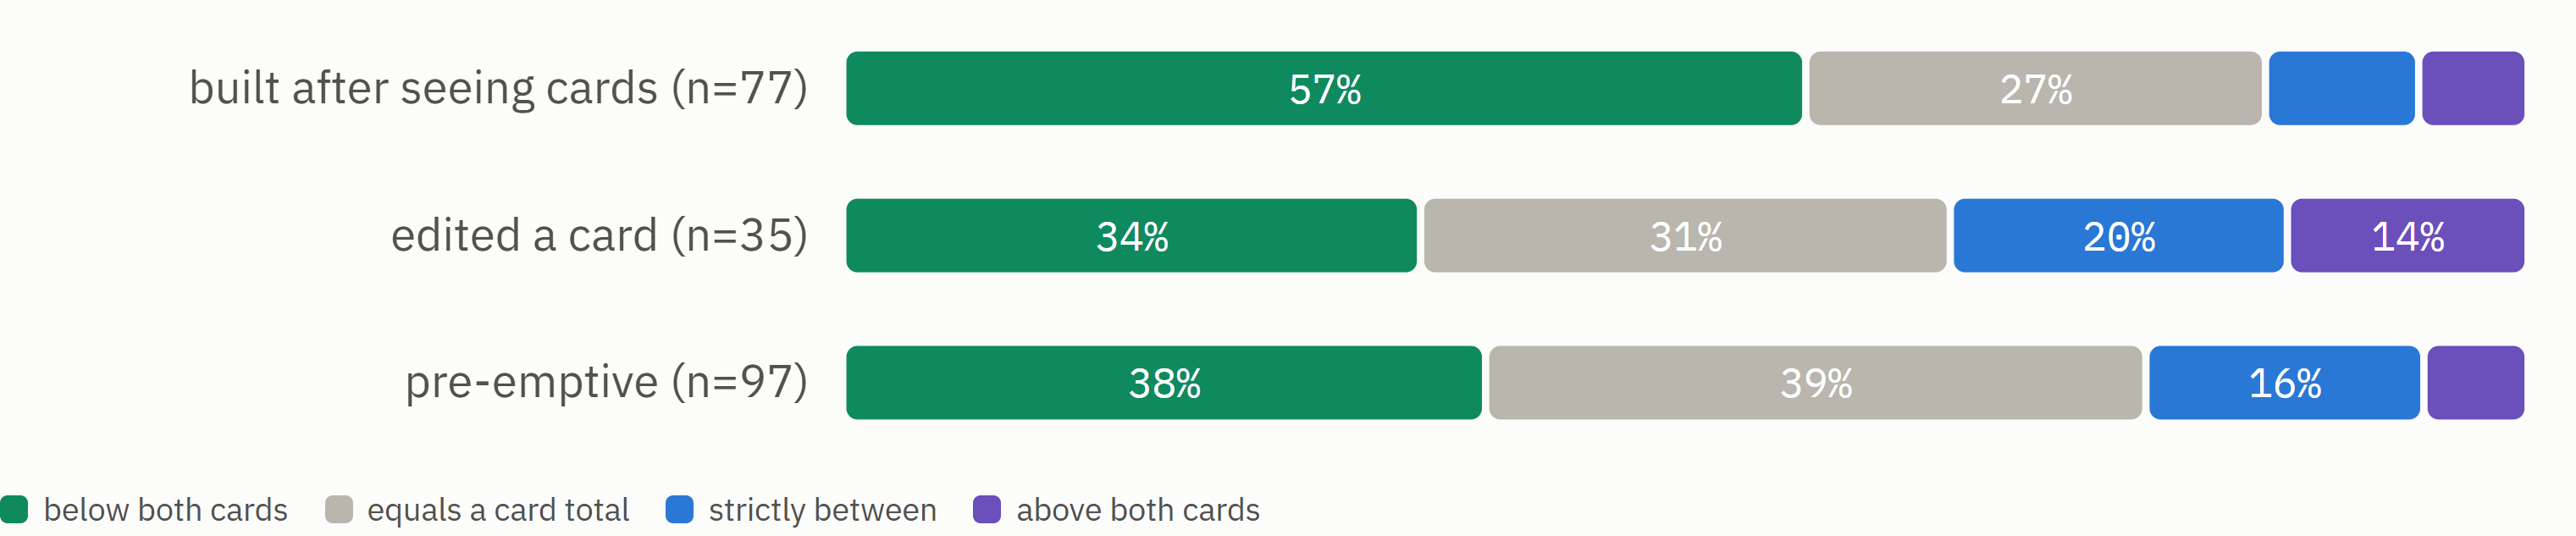
\includegraphics[width=\linewidth,height=0.50\textheight,keepaspectratio]{figs/results/f-manual-cards__position__raw.png}
\caption{\textbf{Hand-built allocations mostly sit below both strategy cards or equal to one, rarely above.}}
\label{fig:res:manual-cards:position}
\label{fig:res:manual-cards:position:raw}
\end{figure}

\begin{options}
\optshead{Options for this finding}

\optsec{Each manual decision against the Conservative card} {\footnotesize [pass 5: for the paper]}

\noindent Key numbers:\begin{itemize}[leftmargin=1.2em,itemsep=0pt]\footnotesize
\item Mean manual $-$ Conservative: $-$0.55 drones overall = $-$0.51 on unneeded types + $-$0.04 on needed types
\item One-type missions: $-$1.17 overall, +0.05 on needed types, $-$1.22 on unneeded; three-type with 10+ drones: +0.95
\item Per doubling of mission size the difference grows by +1.51 drones [0.53, 2.49] (after seeing the cards) and +1.09 [0.47, 1.72] (pre-emptive): the size pattern is just as strong in people who never saw the cards, so it is not a reaction to the card
\item Needed types only, after seeing the cards: +0.93 per doubling [$-$0.18, 2.04], p = .10
\end{itemize}

\noindent Highlighted quotes not used above:\begin{quotelist}
\item ``I'm trying to reserve more and more drones in the base, rather than send them out to finish the task quickly, because I cannot predict when the next task will appear.''\,---\,P28 (debrief 0:28:05)
\end{quotelist}

\optsec{Where manual builds sit relative to the two cards} {\footnotesize [pass 5: for the paper]}

\par\noindent \begin{minipage}[t]{0.49\linewidth}\centering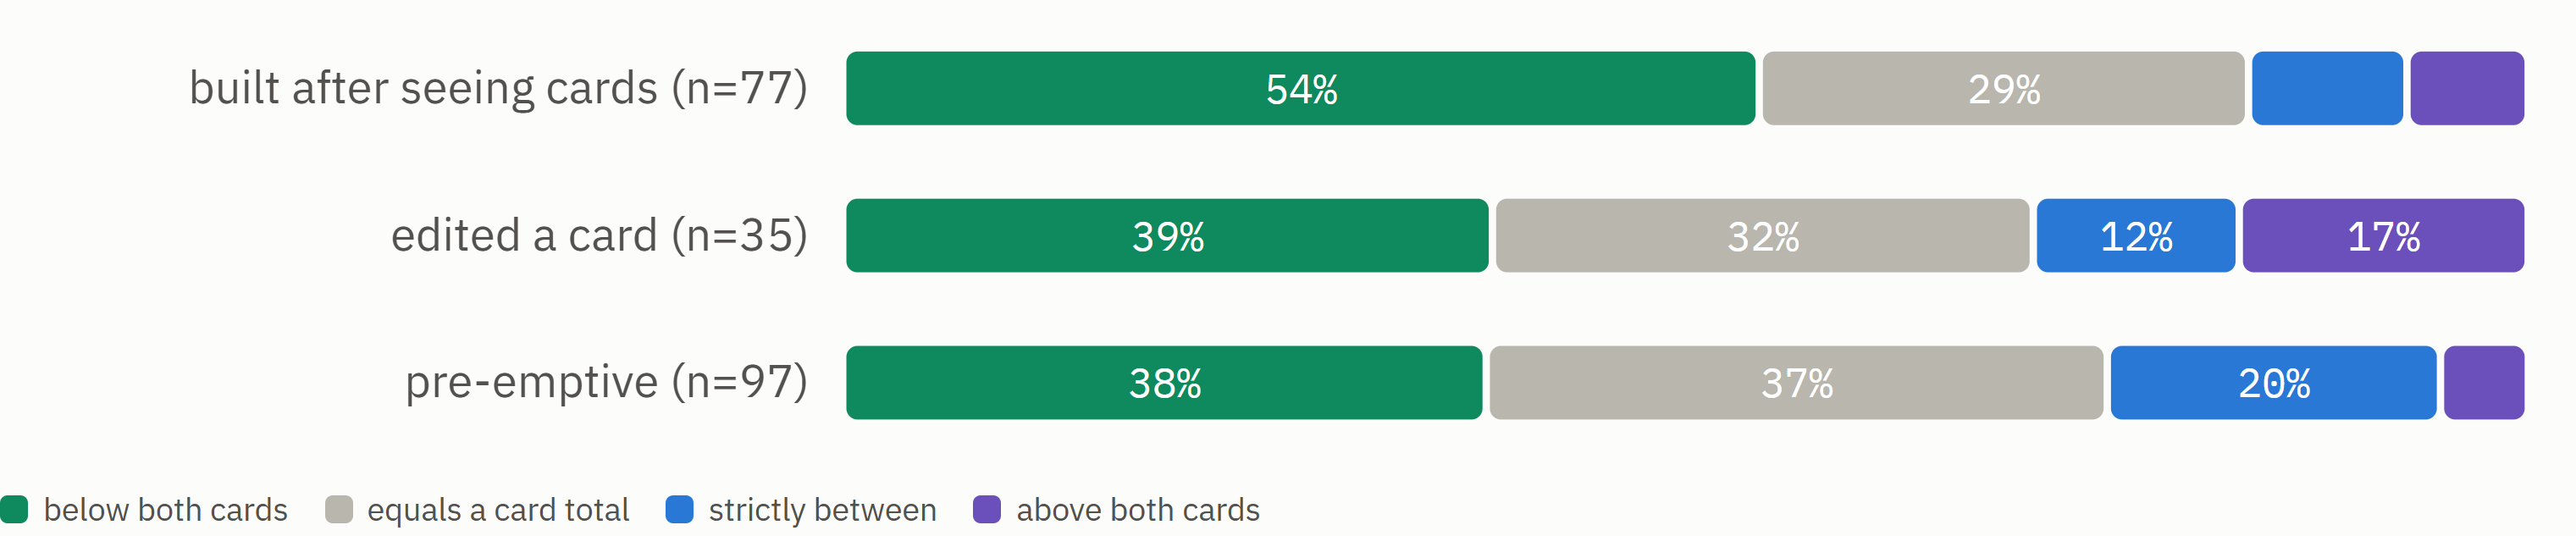
\includegraphics[width=\linewidth,height=0.24\textheight,keepaspectratio]{figs/results/f-manual-cards__position__balanced.png}\par{\scriptsize Other view: Balanced for mission size, drone types, the gap between the cards, game, session and minute.}\end{minipage}

\noindent Key numbers:\begin{itemize}[leftmargin=1.2em,itemsep=0pt]\footnotesize
\item All 209: below both 44\%, equal to a card 33\%, strictly between 14\%, above both 8\%
\item Built after seeing (77): 57\% below, 27\% equal, 9\% between, 6\% above; pre-emptive (97): 38\%, 39\%, 16\%, 6\%
\item Mission mix: pre-emptive builds needed 6.9 drones on average (after seeing 7.6, edited 9.3) and 52\% were one drone type (38\%, 23\%).
\item Balanced: after seeing 54\% below, 29\% equal, 9\% between, 7\% above; pre-emptive 38\%, 37\%, 20\%, 5\%; edited a card 39\%, 32\%, 12\%, 17\%.
\item Pre-emptive minus after seeing, balanced: equal to a card +8 points [$-$10, +23] (raw +12); below both $-$16 [$-$33, +4] (raw $-$19).
\end{itemize}

\noindent Highlighted quotes not used above:\begin{quotelist}
\item ``I felt like sometimes I could find like a middle ground that had like maybe a little bit of gambling in there, essentially, that you wouldn't have the necessary coverage.''\,---\,P22 (debrief 0:28:57)
\end{quotelist}

\optsec{What operators say about building by hand}

\noindent Key numbers:\begin{itemize}[leftmargin=1.2em,itemsep=0pt]\footnotesize
\item C07: 55 manual decisions from 6 people, mean +0.36 vs Conservative on needed types, 21 edited cards
\item C08: 40 from 5 people, 10\% strictly between the cards
\item C09: 33 from 4 people, 16 edited cards
\item C10: 40 from 5 people
\end{itemize}
\end{options}

\clearpage

% ======== f-practice ========

\subsection{Practice makes operators faster, not better at choosing when to hand over}\label{sec:res:practice}

Decisions sped up within each session, by about 6\% per minute on both tiers, and not because the queue grew. On the strategic tier most of that gain was gone by the start of the next session, so it reads as a warm-up within a session more than lasting learning; on the tactical tier the second session started about where the first ended. The size rule did not sharpen with practice.

% --- f-practice#speed (pass 5: numbers only) ---

\phantomsection\label{sec:res:practice:speed}
Figure~\ref{fig:res:practice:speed} shows the median decision time through each session. Strategic decisions fell from 11.6\,s in the first two minutes of session 1 to 6.9\,s at its end, started session 2 nearly as slow again (10.6\,s) and fell once more (5.8\,s). Tactical plans fell from 18.0 to 12.9\,s in session 1 and from 15.5 to 8.0\,s in session 2. Holding the number of waiting missions fixed does not remove the speed-up. Participants described finding a rhythm: ``there was definitely an improvement further throughout session one, and in session two, you really find your stride'' (P10).

\begin{figure}[H]
\centering
\begin{subfigure}[t]{\linewidth}
\centering
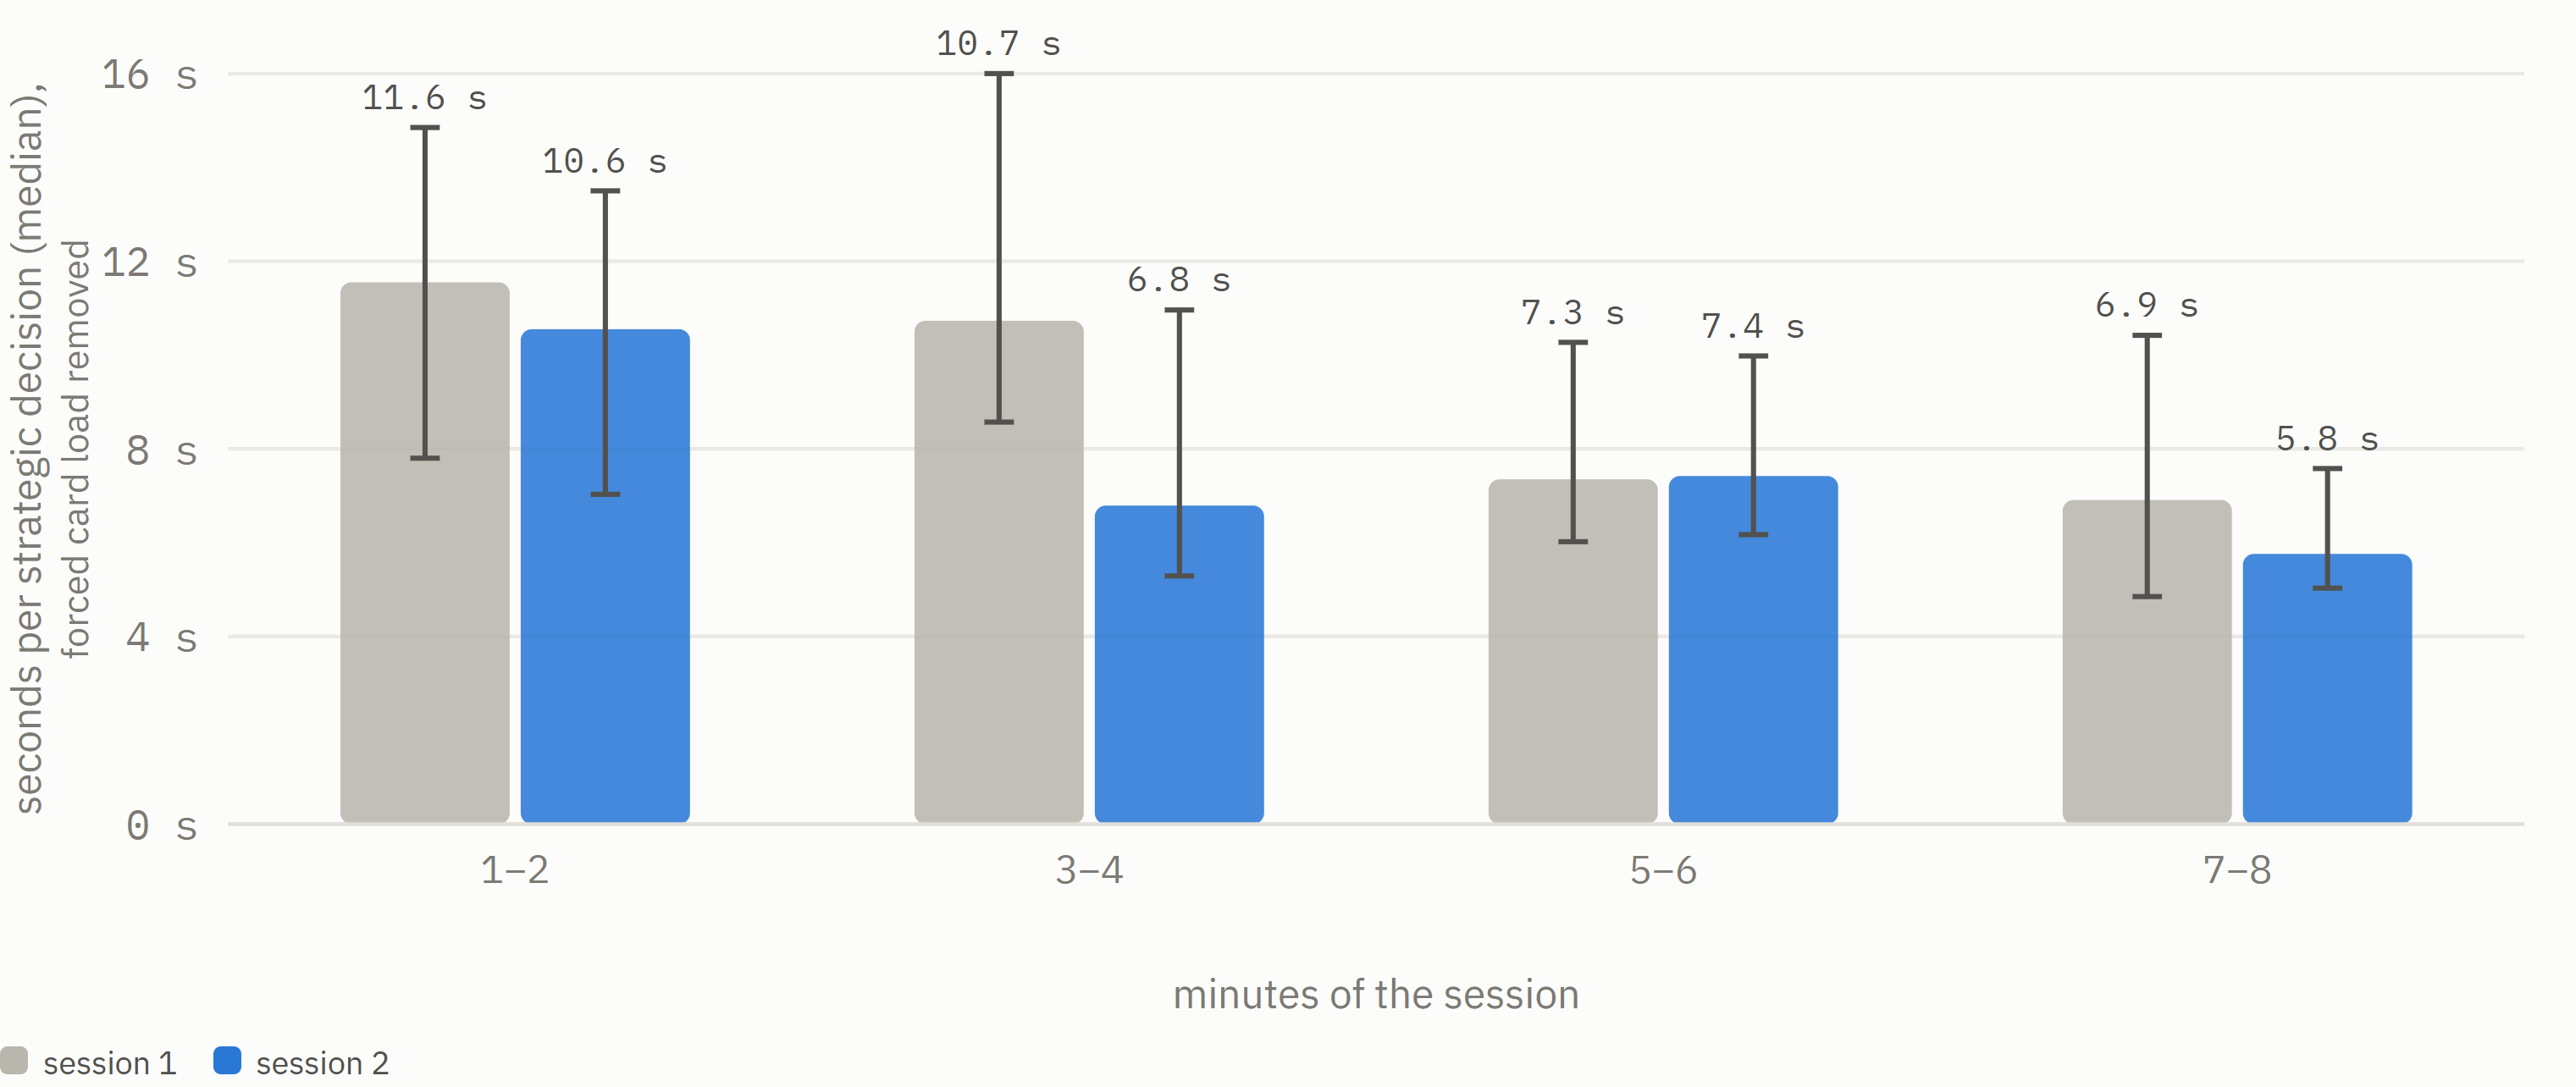
\includegraphics[width=\linewidth,height=0.21\textheight,keepaspectratio]{figs/results/f-practice__speed__strat.png}
\caption{Strategic tier, sessions side by side.}
\label{fig:res:practice:speed:strat}
\end{subfigure}
\par\smallskip
\begin{subfigure}[t]{\linewidth}
\centering
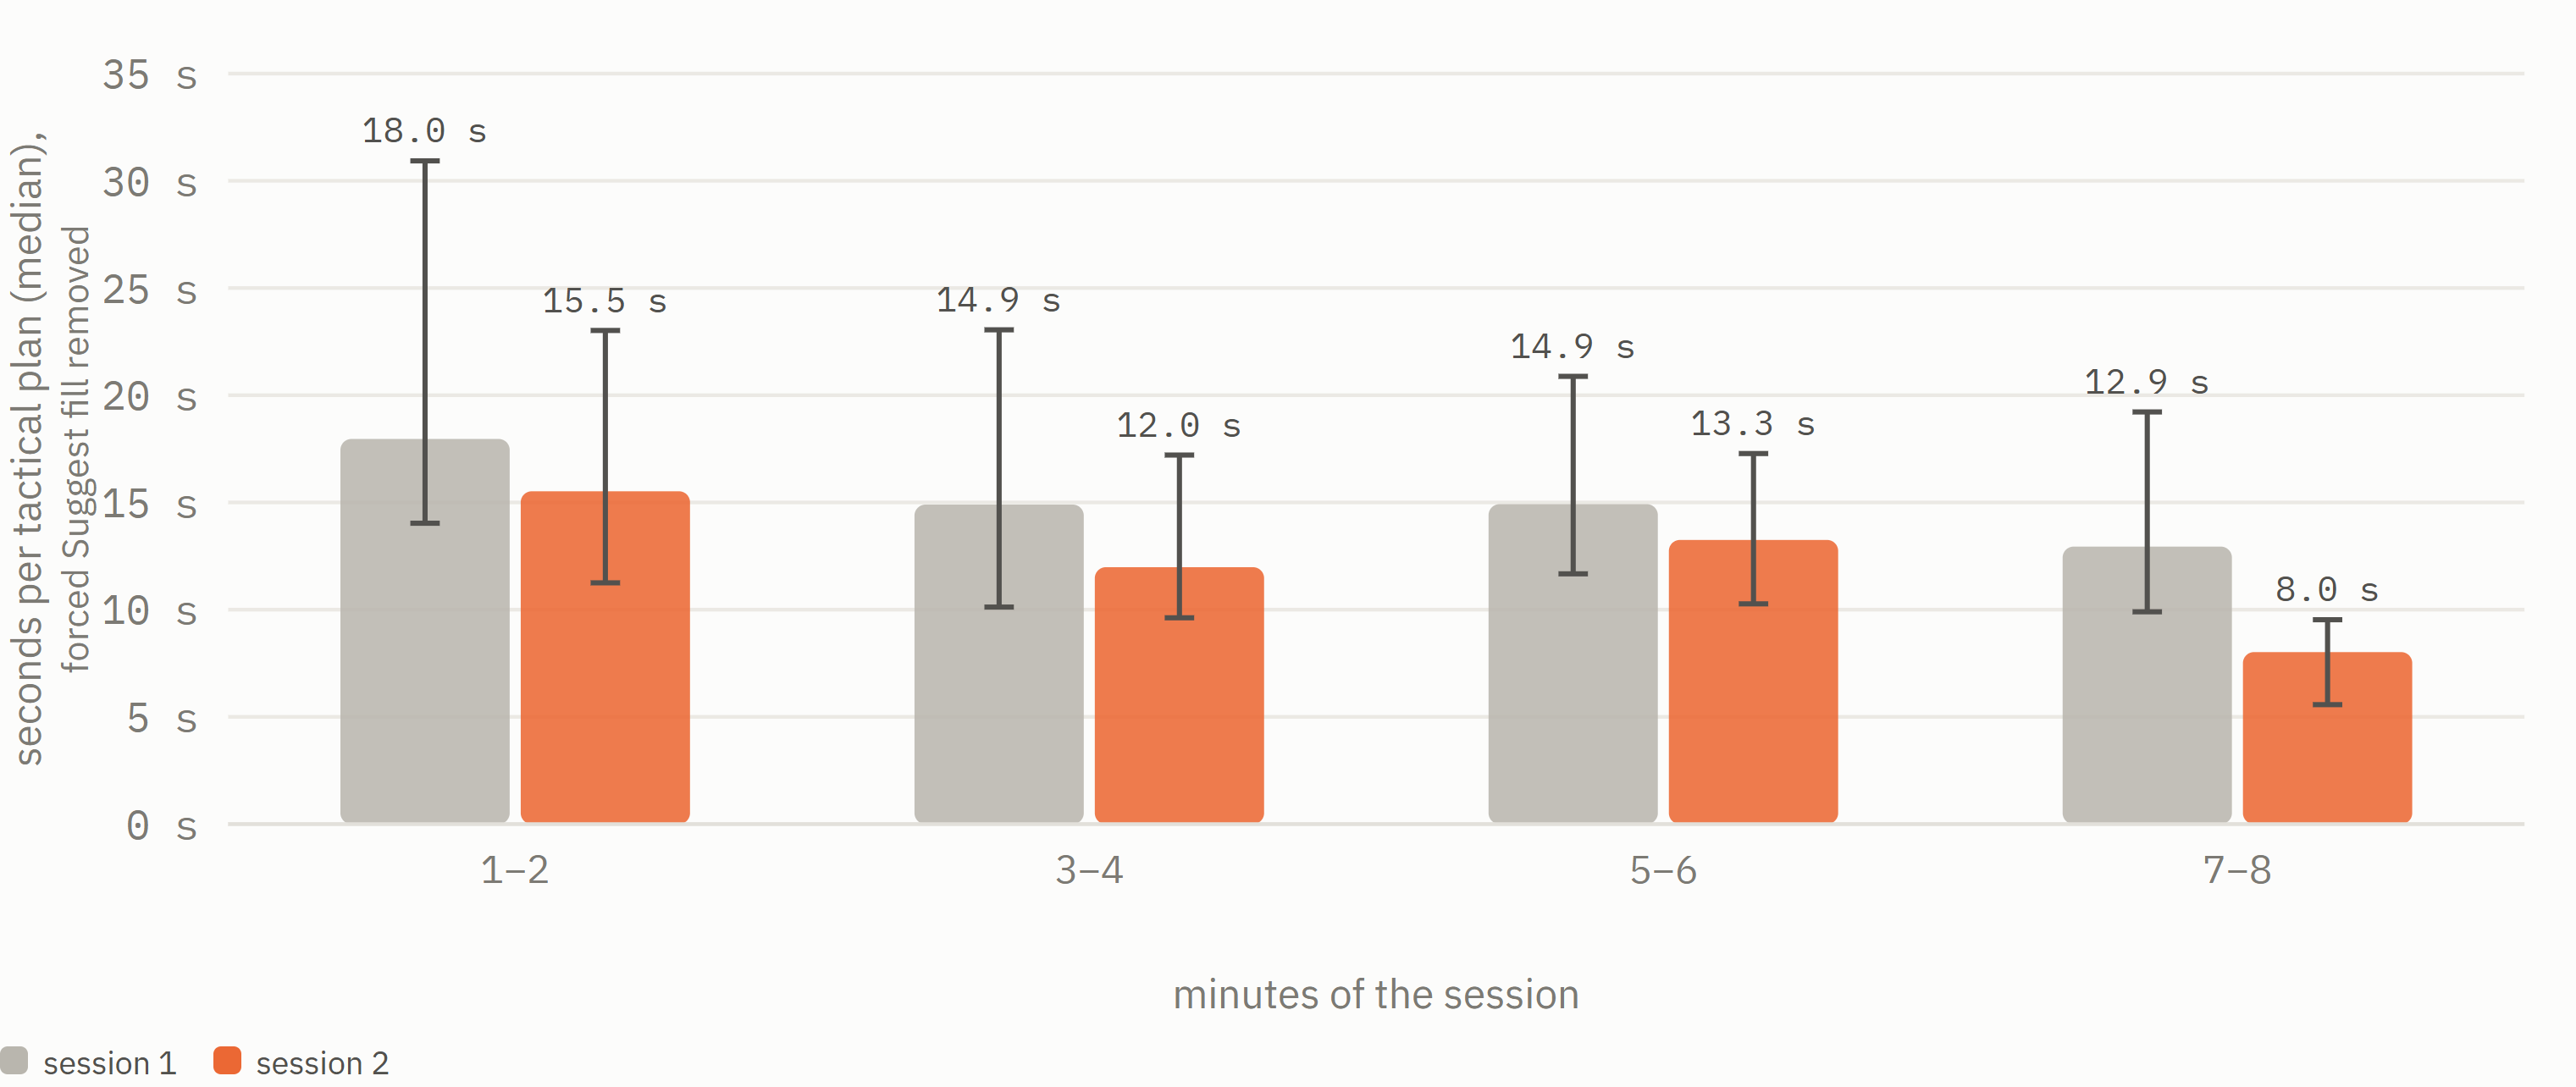
\includegraphics[width=\linewidth,height=0.21\textheight,keepaspectratio]{figs/results/f-practice__speed__tac.png}
\caption{Tactical tier, sessions side by side.}
\label{fig:res:practice:speed:tac}
\end{subfigure}
\par\smallskip
\caption{\textbf{Faster within a session; on the strategic tier the gain mostly resets by the next.} Median time per decision by pair of minutes: (a) strategic tier, (b) tactical tier.}
\label{fig:res:practice:speed}
\end{figure}

% --- f-practice#c22 (pass 5: numbers only) ---

\phantomsection\label{sec:res:practice:c22}
The six participants who said they got better did improve their scores (all six, against 10 of the other 27), but they did not come to use the assistants more, and across everyone a bigger score gain did not go with more use of either assistant ($\rho = -.07$ for strategy cards, $-.18$ for tactical suggestions).

\begin{options}
\optshead{Options for this finding}

\optsec{Faster within a session; on the strategic tier the gain mostly resets by the next} {\footnotesize [pass 5: numbers only]}

\par\noindent \begin{minipage}[t]{0.49\linewidth}\centering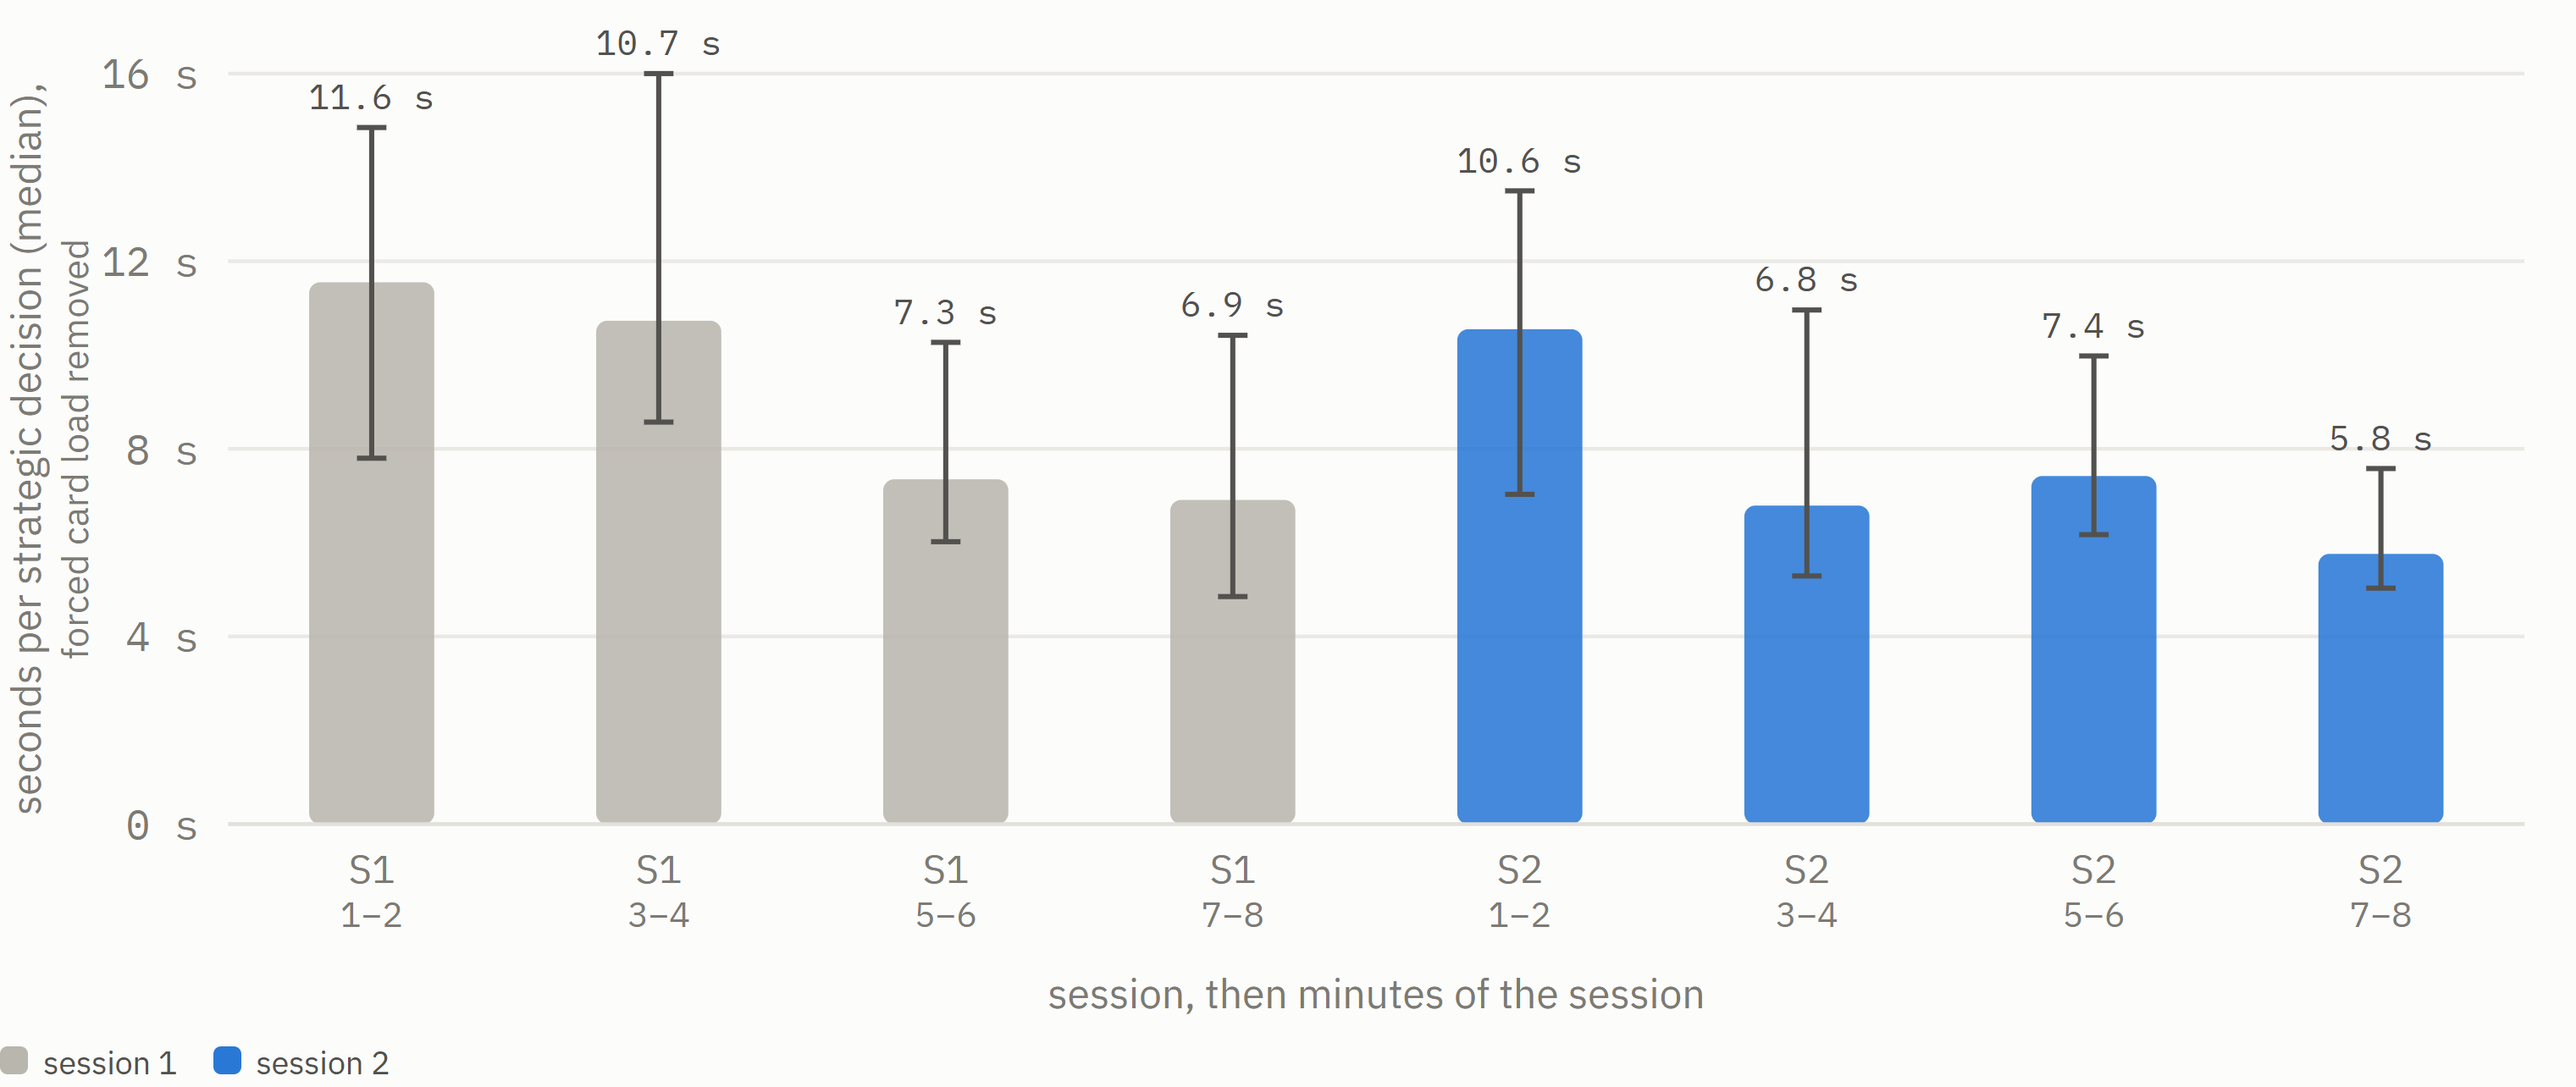
\includegraphics[width=\linewidth,height=0.24\textheight,keepaspectratio]{figs/results/f-practice__speed__strat-order.png}\par{\scriptsize Other view: Strategic tier, all of session 1 then all of session 2.}\end{minipage}

\noindent Key numbers:\begin{itemize}[leftmargin=1.2em,itemsep=0pt]\footnotesize
\item Strategic, medians: session 1 minutes 1--2 11.6 s [7.8, 14.5] $\rightarrow$ minutes 7--8 6.9 s [4.9, 10.2]; session 2 10.6 s [7.0, 13.5] $\rightarrow$ 5.8 s [5.0, 7.6]
\item Strategic, model: end of session 1 $-$39\% [$-$51, $-$24]; start of session 2 $-$20\% [$-$37, +2], p = .07; start of session 2 vs end of session 1 +31\% [0, +72], p = .053 (slower again)
\item Tactical, medians: 18.0 s [14.0, 30.9] $\rightarrow$ 12.9 s [10.1, 19.2]; session 2 15.5 s [11.3, 21.9] $\rightarrow$ 8.0 s [5.6, 9.6]
\item Tactical, model: end of session 1 $-$24\% [$-$45, +4], p = .09; start of session 2 vs end of session 1 +2\% [$-$33, +56], p = .92; session 2 slope $-$7\% per minute vs $-$4\% in session 1 (difference p = .26)
\item Within-session slope with the queue held fixed: strategic $-$6\% per minute, tactical $-$8\% per minute (both p < .001)
\item Overall (unchanged): strategic $-$5.7\% per minute [$-$7.8, $-$3.6], session 2 vs 1 $-$19\% [$-$30, $-$6]; tactical $-$5.7\% per minute [$-$9.1, $-$2.2], session 2 vs 1 $-$24\% [$-$36, $-$9]
\end{itemize}

\noindent Highlighted quotes not used above:\begin{quotelist}
\item ``i think the second scenario i used more personalised, i think it was easier because i had to i sort of got into the rhythm of having to anticipate other problems''\,---\,P30 (debrief 0:23:52)
\item ``Right. So now we also know from the last one, don't send everything straight away. Cause otherwise we end up, we're waiting for drones.''\,---\,P22 (think-aloud s2 0:17:11)
\item ``And I could definitely feel that there is absolutely a learning effect.''\,---\,P10 (debrief 0:22:39)
\item ``I think with having some experience, yeah, I was able to quickly understand this''\,---\,P05 (think-aloud s1 0:11:14)
\end{quotelist}

\optsec{Does 'I got better with practice' match the logs? For score yes; not for speed or assistant use} {\footnotesize [pass 5: numbers only]}

\par\noindent \begin{minipage}[t]{0.49\linewidth}\centering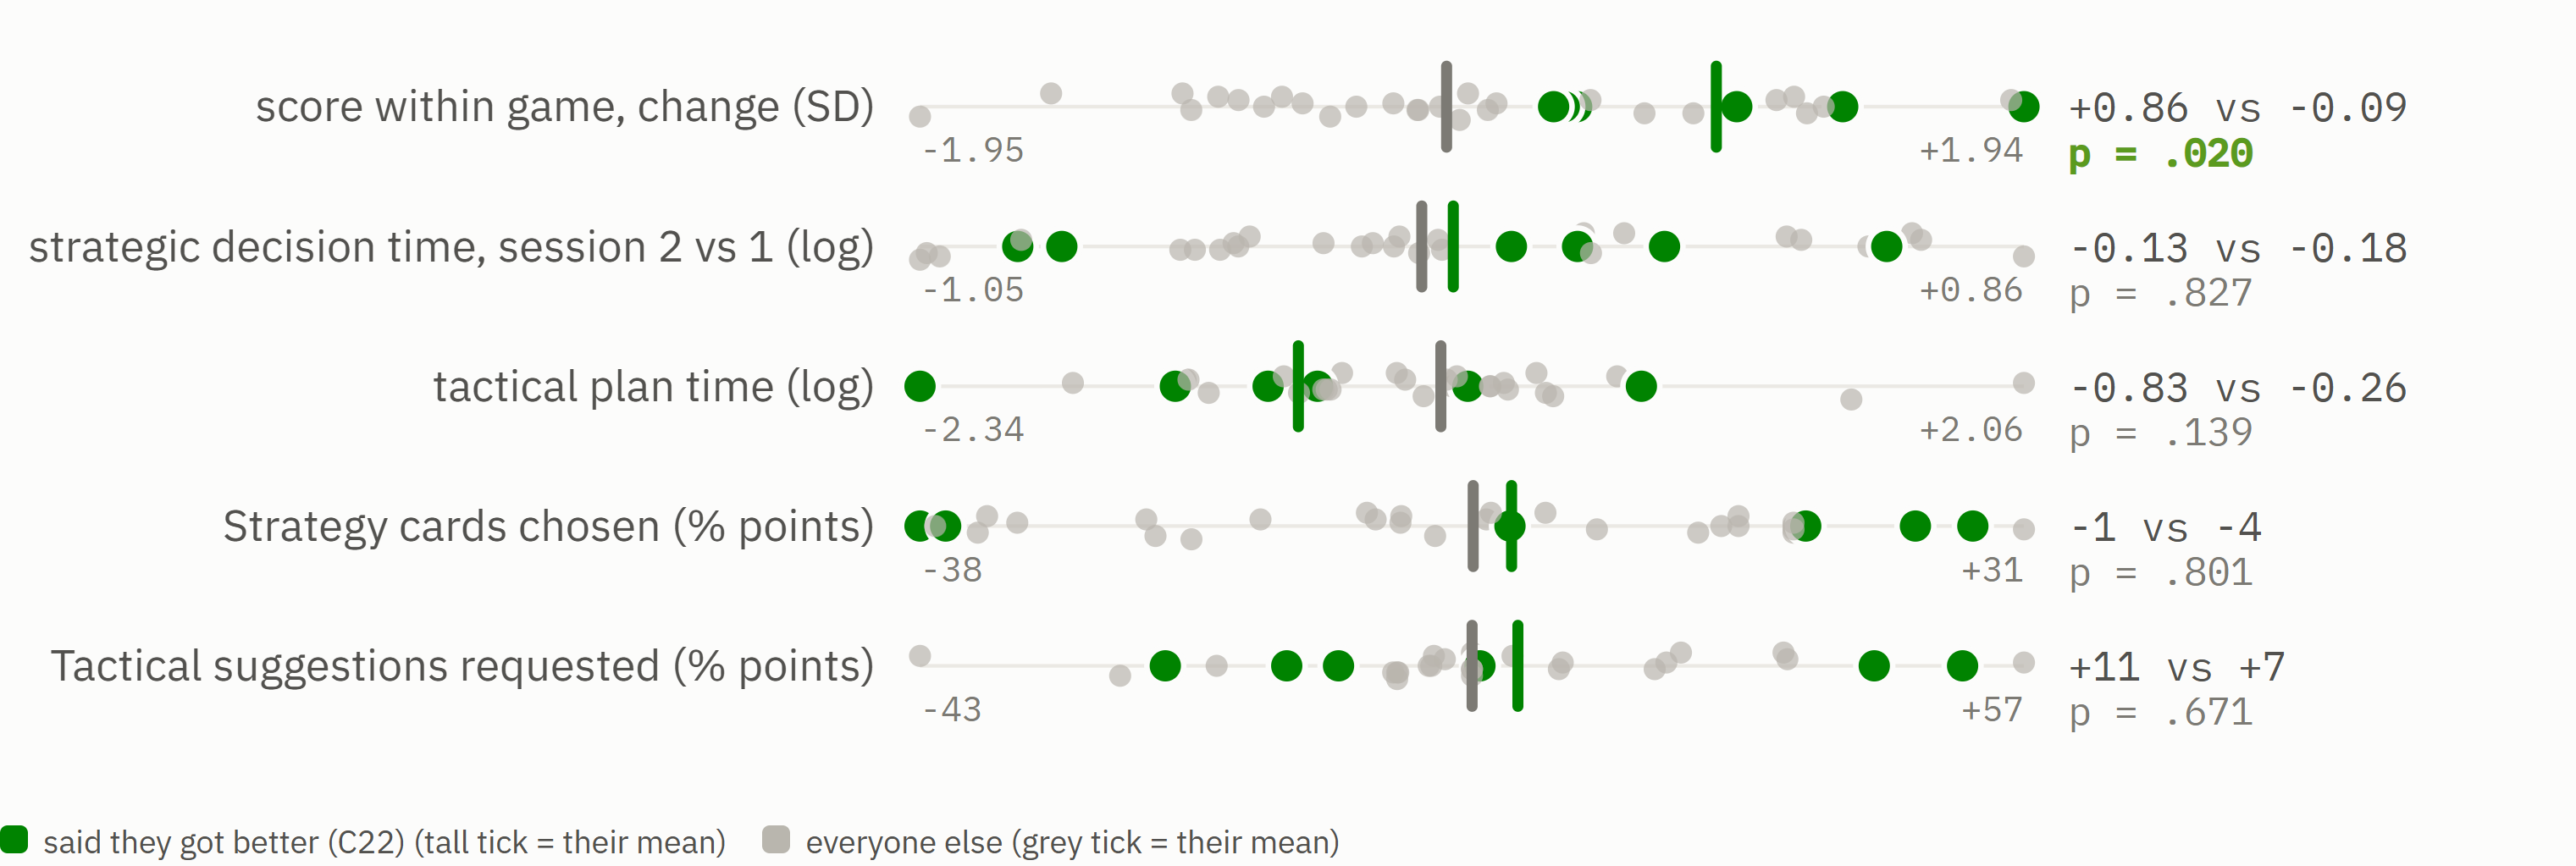
\includegraphics[width=\linewidth,height=0.24\textheight,keepaspectratio]{figs/results/f-practice__c22__main.png}\par{\scriptsize Other view: main}\end{minipage}

\noindent Key numbers:\begin{itemize}[leftmargin=1.2em,itemsep=0pt]\footnotesize
\item Score change: C22 +0.86 SD vs others $-$0.09, p = .020
\item Tactical time change (log): $-$0.83 vs $-$0.26, p = .14; strategic: $-$0.13 vs $-$0.18, p = .83
\item Change in strategy cards chosen (game-adjusted): C22 $-$1 point vs others $-$4, p = .80; suggestion requested: +11 vs +7 points, p = .67
\item Used more in session 2: cards 3 of 6 C22 vs 12 of 27 others; Suggest 3 of 6 vs 19 of 27
\item Everyone: score change vs change in strategy card choice $\rho$ = $-$.07 (p = .71); vs change in Suggest $\rho$ = $-$.18 (p = .32)
\end{itemize}
\end{options}

\clearpage

% ======== f-workload ========

\subsection{A busier moment does not push operators onto the assistants}\label{sec:res:workload}

Comparing each operator with themselves, having more missions waiting did not change how often they chose a strategy card or requested a tactical suggestion, once we account for what each decision was, when it came in the session, which game it was and who made it. The data rule out large effects (on the strategic tier, at most about 15 points more strategy card choice going from zero to five missions waiting). Nine of 33 participants said they handed over more when overloaded; their own behaviour moved with the queue no more than anyone else's.

% --- f-workload#raw-vs-adjusted (pass 5: for the paper) ---

\phantomsection\label{sec:res:workload:raw-vs-adjusted}
Figure~\ref{fig:res:workload:raw-vs-adjusted} shows the share of decisions handed over by the number of other missions waiting. The raw strategic rate dips at three to four missions waiting, but that dip is where the decisions themselves predicted it (dashed lines): deep queues happened almost only in the Strategic Heavy games and late in a session. Adjusted for the mission, the minute, the game and the person, every point sits between 59\% and 74\% on the strategic tier and between 75\% and 82\% on the tactical tier, with no trend, including beyond the point where the queue list runs out of room. This runs against what participants said, for example: ``So I think if, at first glance, I felt really overwhelmed by the amount of drones to be assigned. I would use the assistant'' (P18).

\begin{figure}[H]
\centering
\begin{subfigure}[t]{\linewidth}
\centering
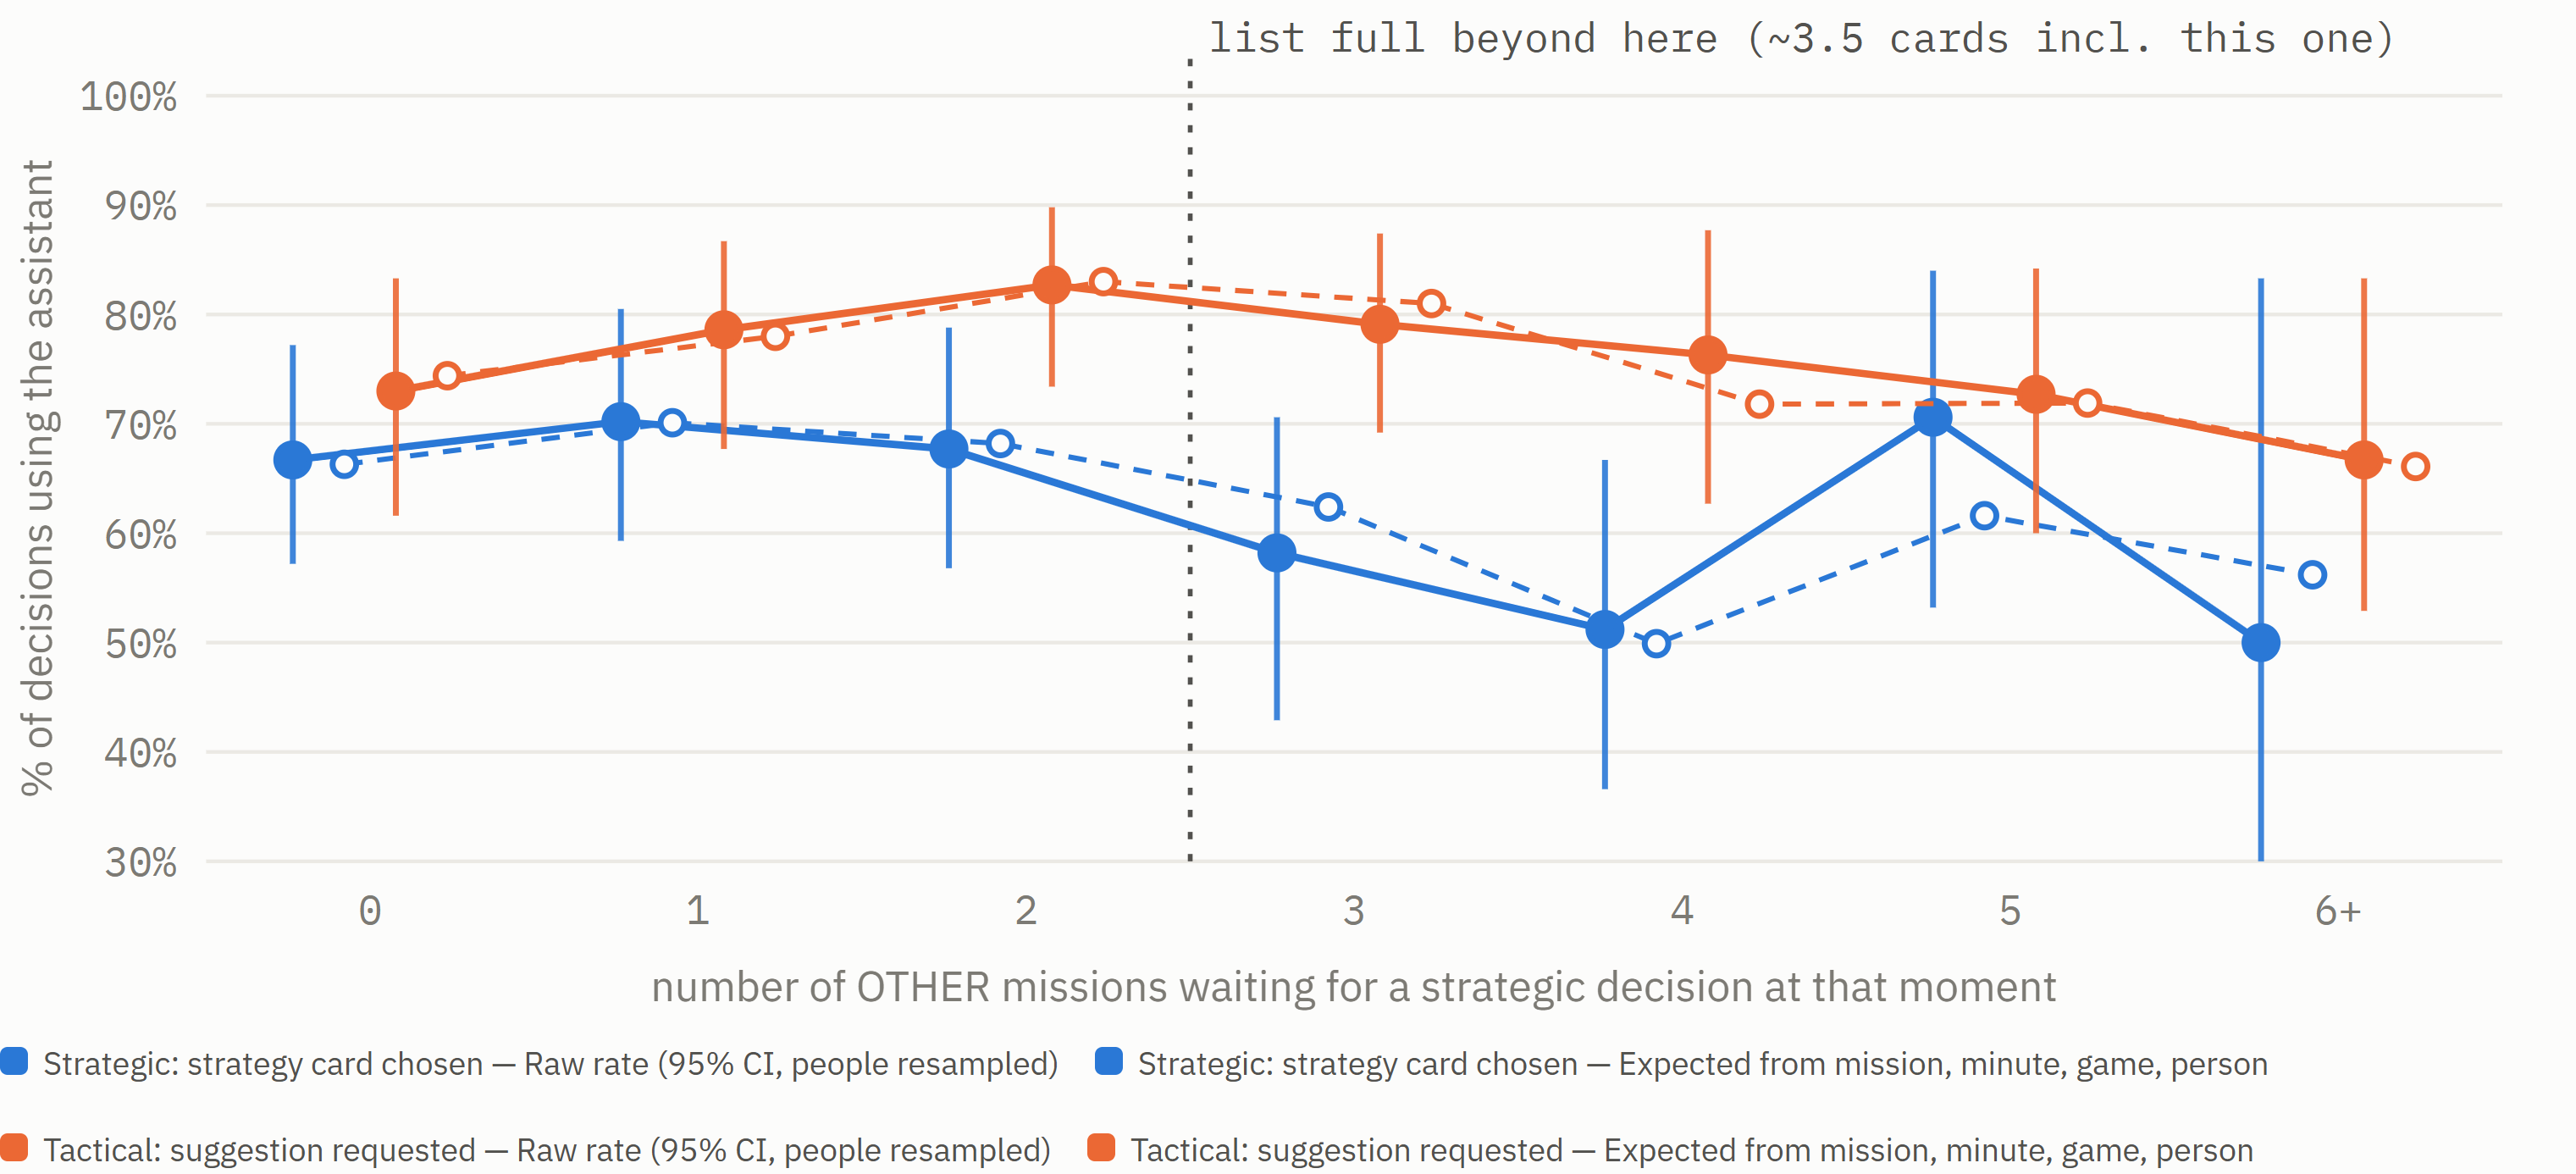
\includegraphics[width=\linewidth,height=0.21\textheight,keepaspectratio]{figs/results/f-workload__raw-vs-adjusted__both-exp.png}
\caption{Both tiers together, raw with their expected rates (dashed).}
\label{fig:res:workload:raw-vs-adjusted:both-exp}
\end{subfigure}
\par\smallskip
\begin{subfigure}[t]{\linewidth}
\centering
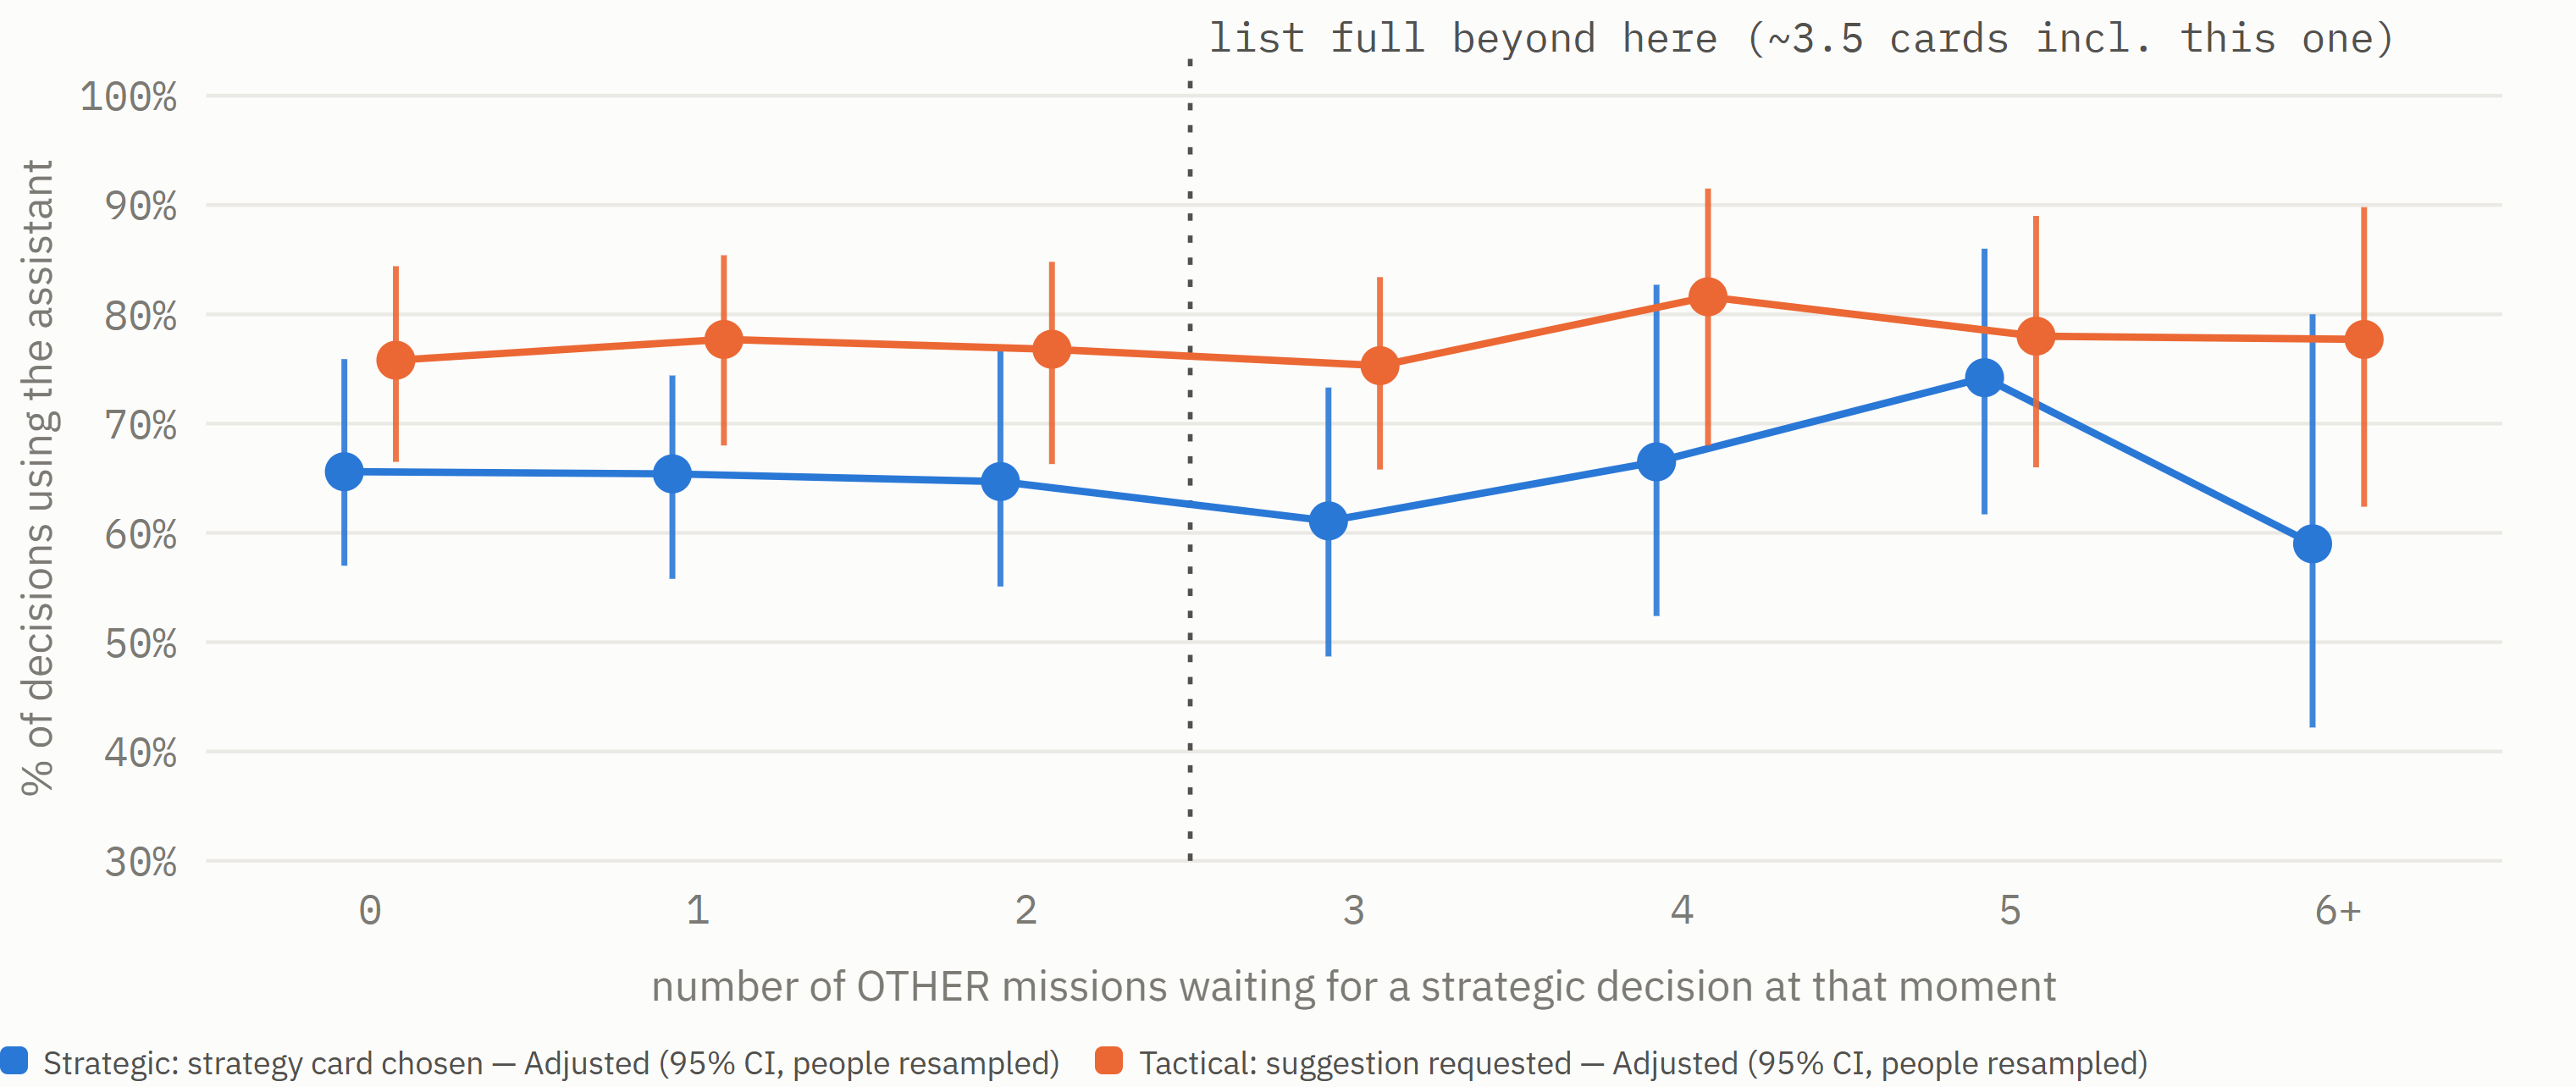
\includegraphics[width=\linewidth,height=0.21\textheight,keepaspectratio]{figs/results/f-workload__raw-vs-adjusted__both-adj.png}
\caption{Both tiers together, adjusted.}
\label{fig:res:workload:raw-vs-adjusted:both-adj}
\end{subfigure}
\par\smallskip
\caption{\textbf{A busier moment does not push operators onto the assistants.} Share of decisions handed over by the number of other missions waiting, both tiers together: (a) raw, with the rate the decisions themselves predict (dashed); (b) adjusted.}
\label{fig:res:workload:raw-vs-adjusted}
\end{figure}

% --- f-workload#waited (pass 5: numbers only) ---

\phantomsection\label{sec:res:workload:waited}
Nor were missions handed over more often after being left waiting: strategy card choice was 63--68\% (adjusted) whether a mission had waited ten seconds or more than two minutes, and tactical suggestions, if anything, became a little less likely the longer a plan had been left open.

\begin{options}
\optshead{Options for this finding}

\optsec{Queue depth against reliance --- raw, and adjusted} {\footnotesize [pass 5: for the paper]}

\par\noindent \begin{minipage}[t]{0.49\linewidth}\centering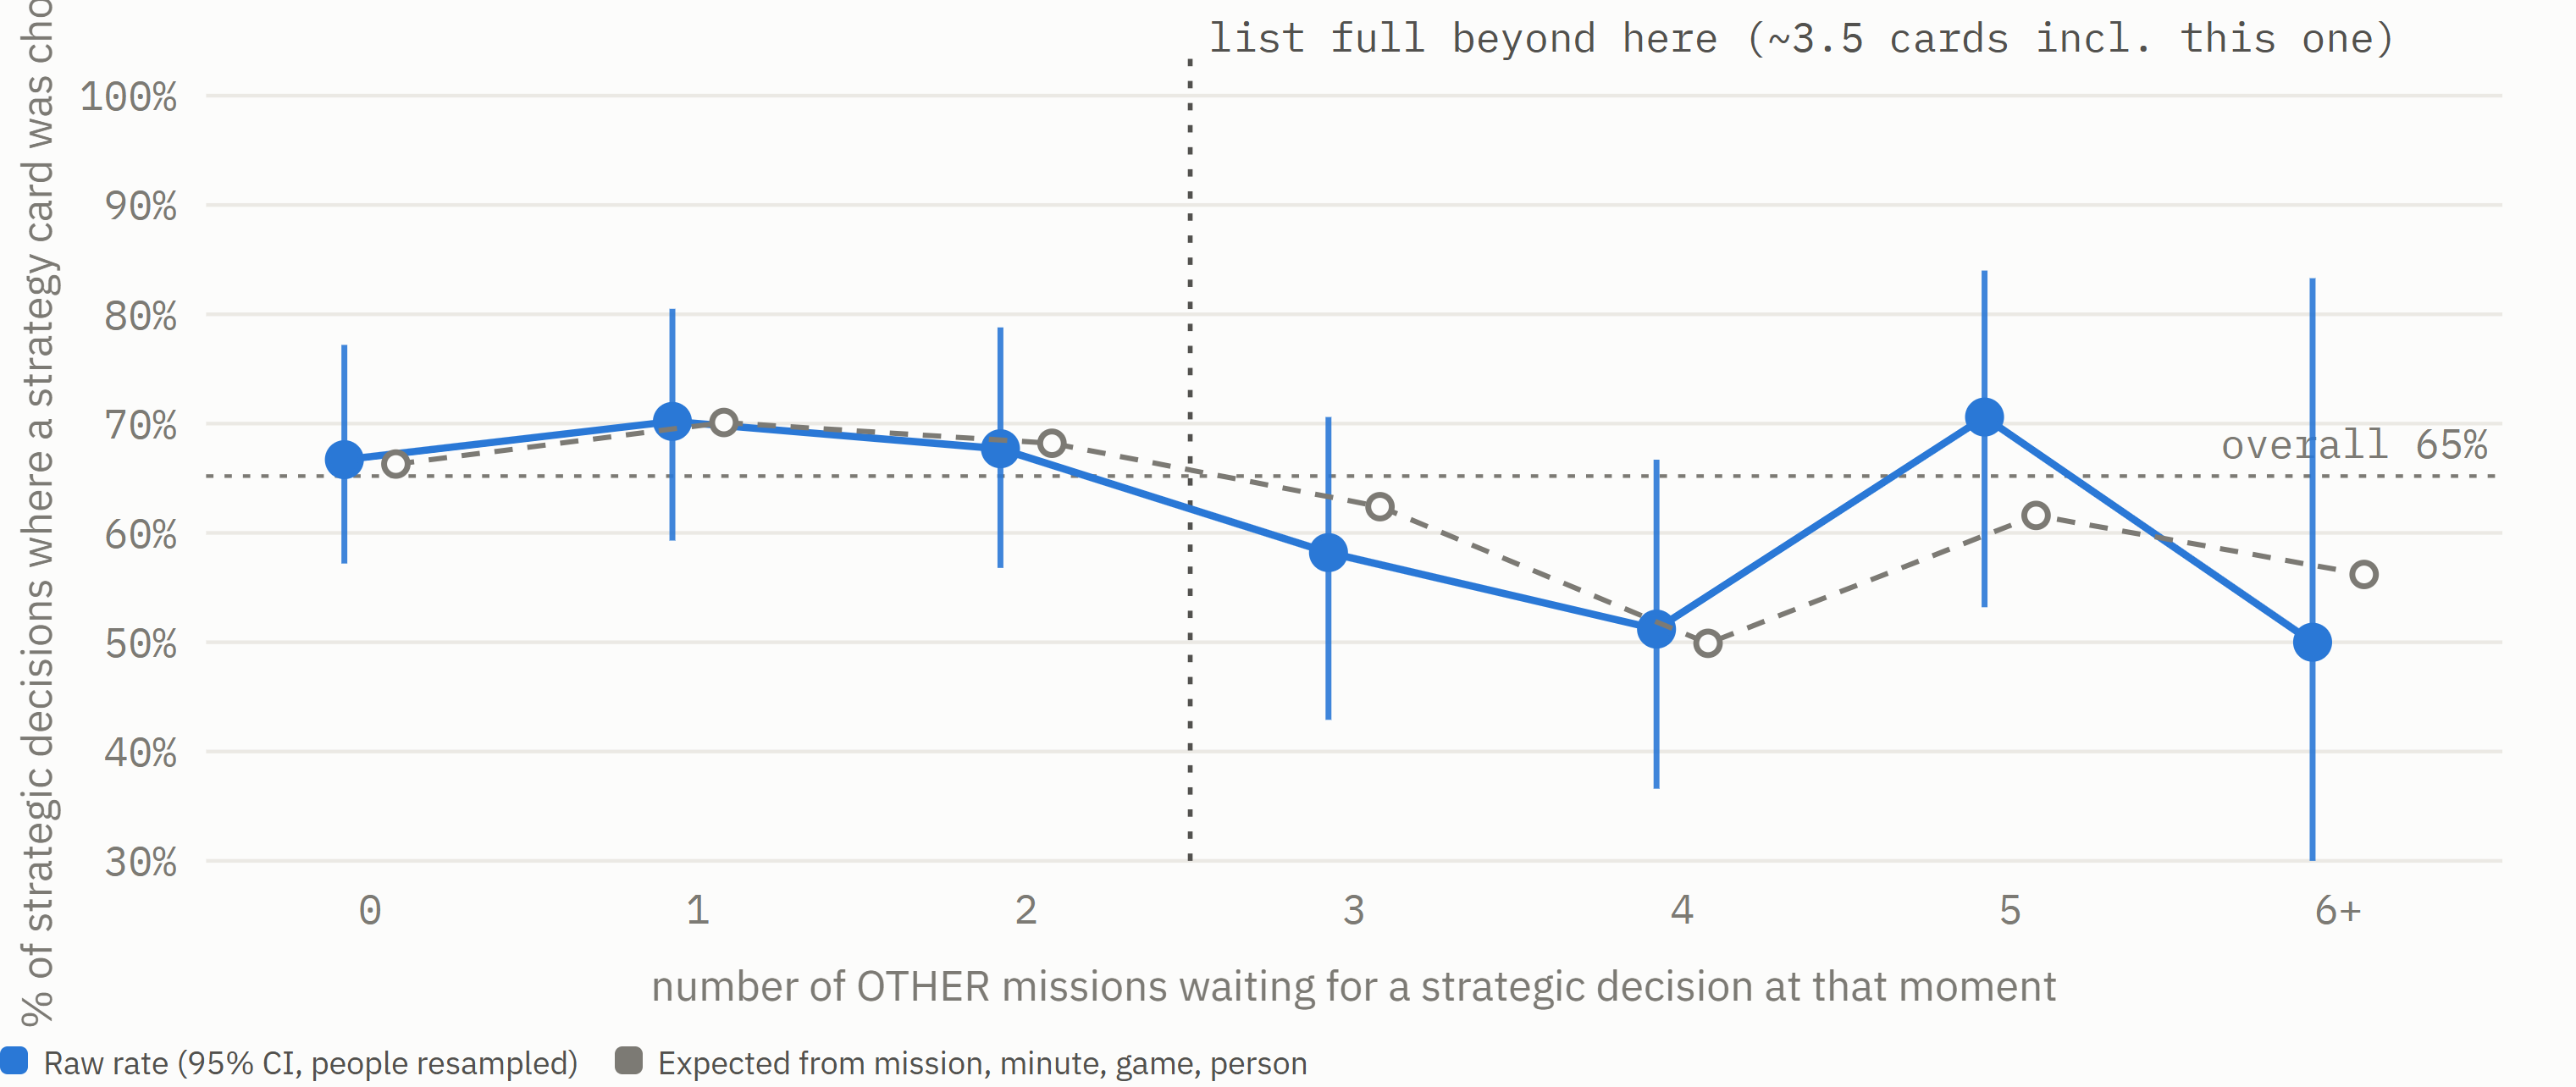
\includegraphics[width=\linewidth,height=0.24\textheight,keepaspectratio]{figs/results/f-workload__raw-vs-adjusted__strat-exp.png}\par{\scriptsize Other view: Strategic tier, raw with the expected rate (dashed).}\end{minipage}\hfill
\begin{minipage}[t]{0.49\linewidth}\centering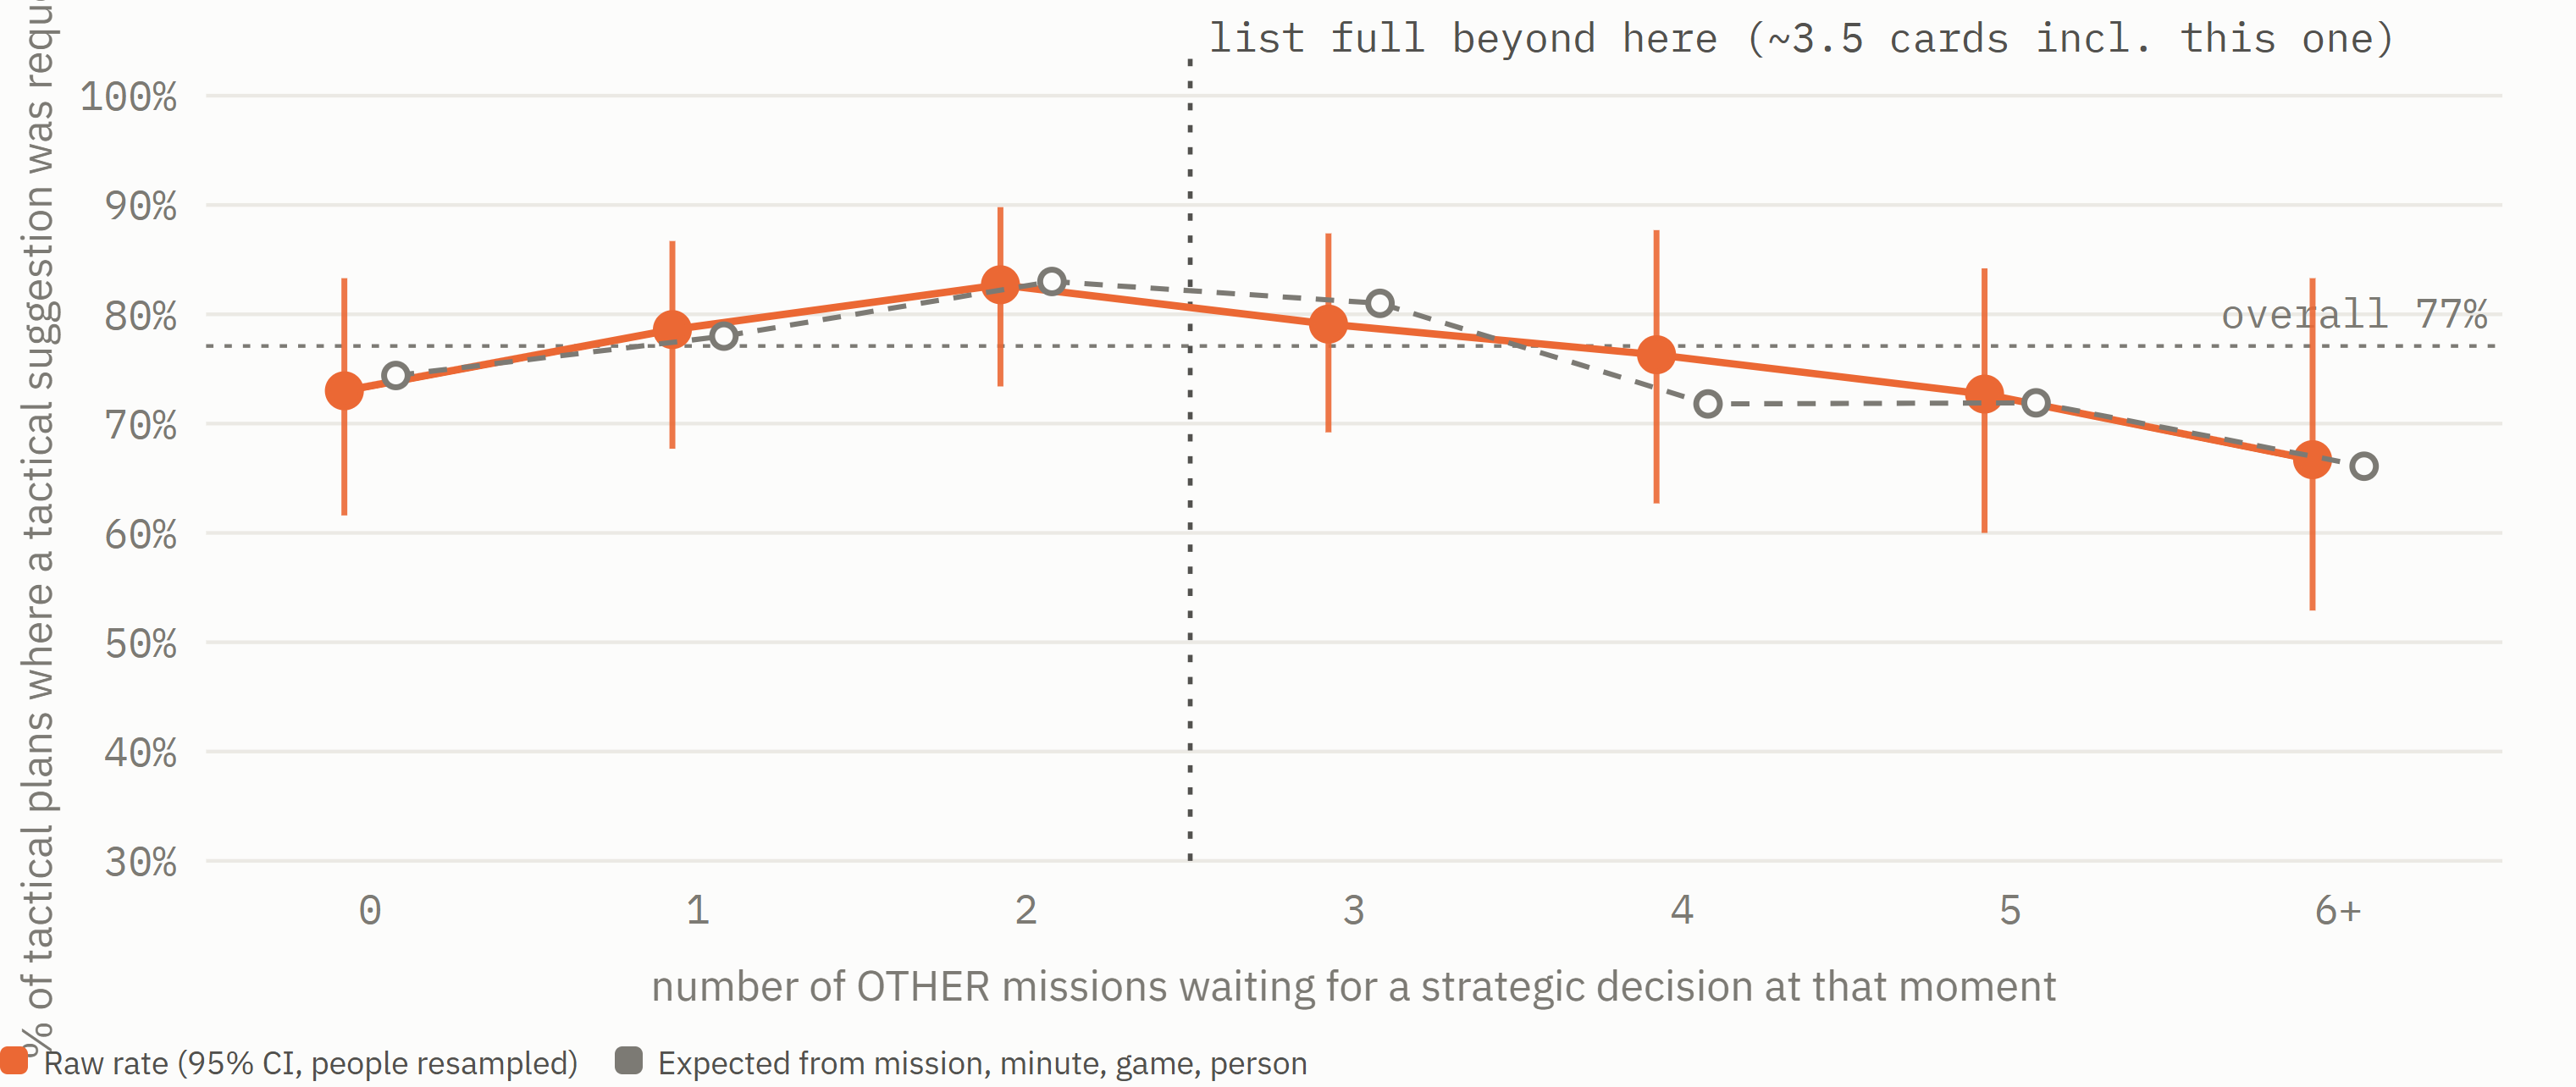
\includegraphics[width=\linewidth,height=0.24\textheight,keepaspectratio]{figs/results/f-workload__raw-vs-adjusted__tac-exp.png}\par{\scriptsize Other view: Tactical tier, raw with the expected rate (dashed).}\end{minipage}

\noindent Key numbers:\begin{itemize}[leftmargin=1.2em,itemsep=0pt]\footnotesize
\item Strategic raw: 67\% (0 waiting), 70\%, 68\%, 58\%, 51\%, 71\%, 50\% (6+); adjusted: 66\%, 65\%, 65\%, 61\%, 67\%, 74\%, 59\% --- all intervals overlap.
\item Tactical raw: 73\%, 79\%, 83\%, 79\%, 76\%, 73\%, 67\%; adjusted: 76\%, 78\%, 77\%, 75\%, 82\%, 78\%, 78\%.
\item The queue rises with the minute (Spearman $\rho$ = .49) but hardly with mission size ($\rho$ = $-$.08): the adjustment mostly removes WHO reaches deep queues and WHICH GAME they are in.
\item Deep queues are a Strategic Heavy phenomenon: 90--97\% of decisions at 4+ waiting are in those two games.
\end{itemize}

\noindent Highlighted quotes not used above:\begin{quotelist}
\item ``You can have a lot of tasks to be overloaded and try and offload some of that work to AI and then for the very complex stuff, maybe you don't.''\,---\,P20 (debrief 0:28:46)
\item ``there was no more active missions coming in, so therefore I could take more time and ensure that it was correct. But perhaps if I was more time pressured, then I'd ask it to suggest.''\,---\,P05 (think-aloud s1 7:31)
\item ``But in an urgent situation and the number of the swarm is not enough, so I need to consider about the strategies and I think I need the help of AI assistant.''\,---\,P35 (debrief 0:28:19)
\item ``I think the first one, I feel the pace is very, very fast. So, I can't do it very well in a very short time. So, I used a lot of AI suggestions.''\,---\,P33 (debrief 0:27:33)
\end{quotelist}

\optsec{A mission left waiting is not handed over more often} {\footnotesize [pass 5: numbers only]}

\par\noindent \begin{minipage}[t]{0.49\linewidth}\centering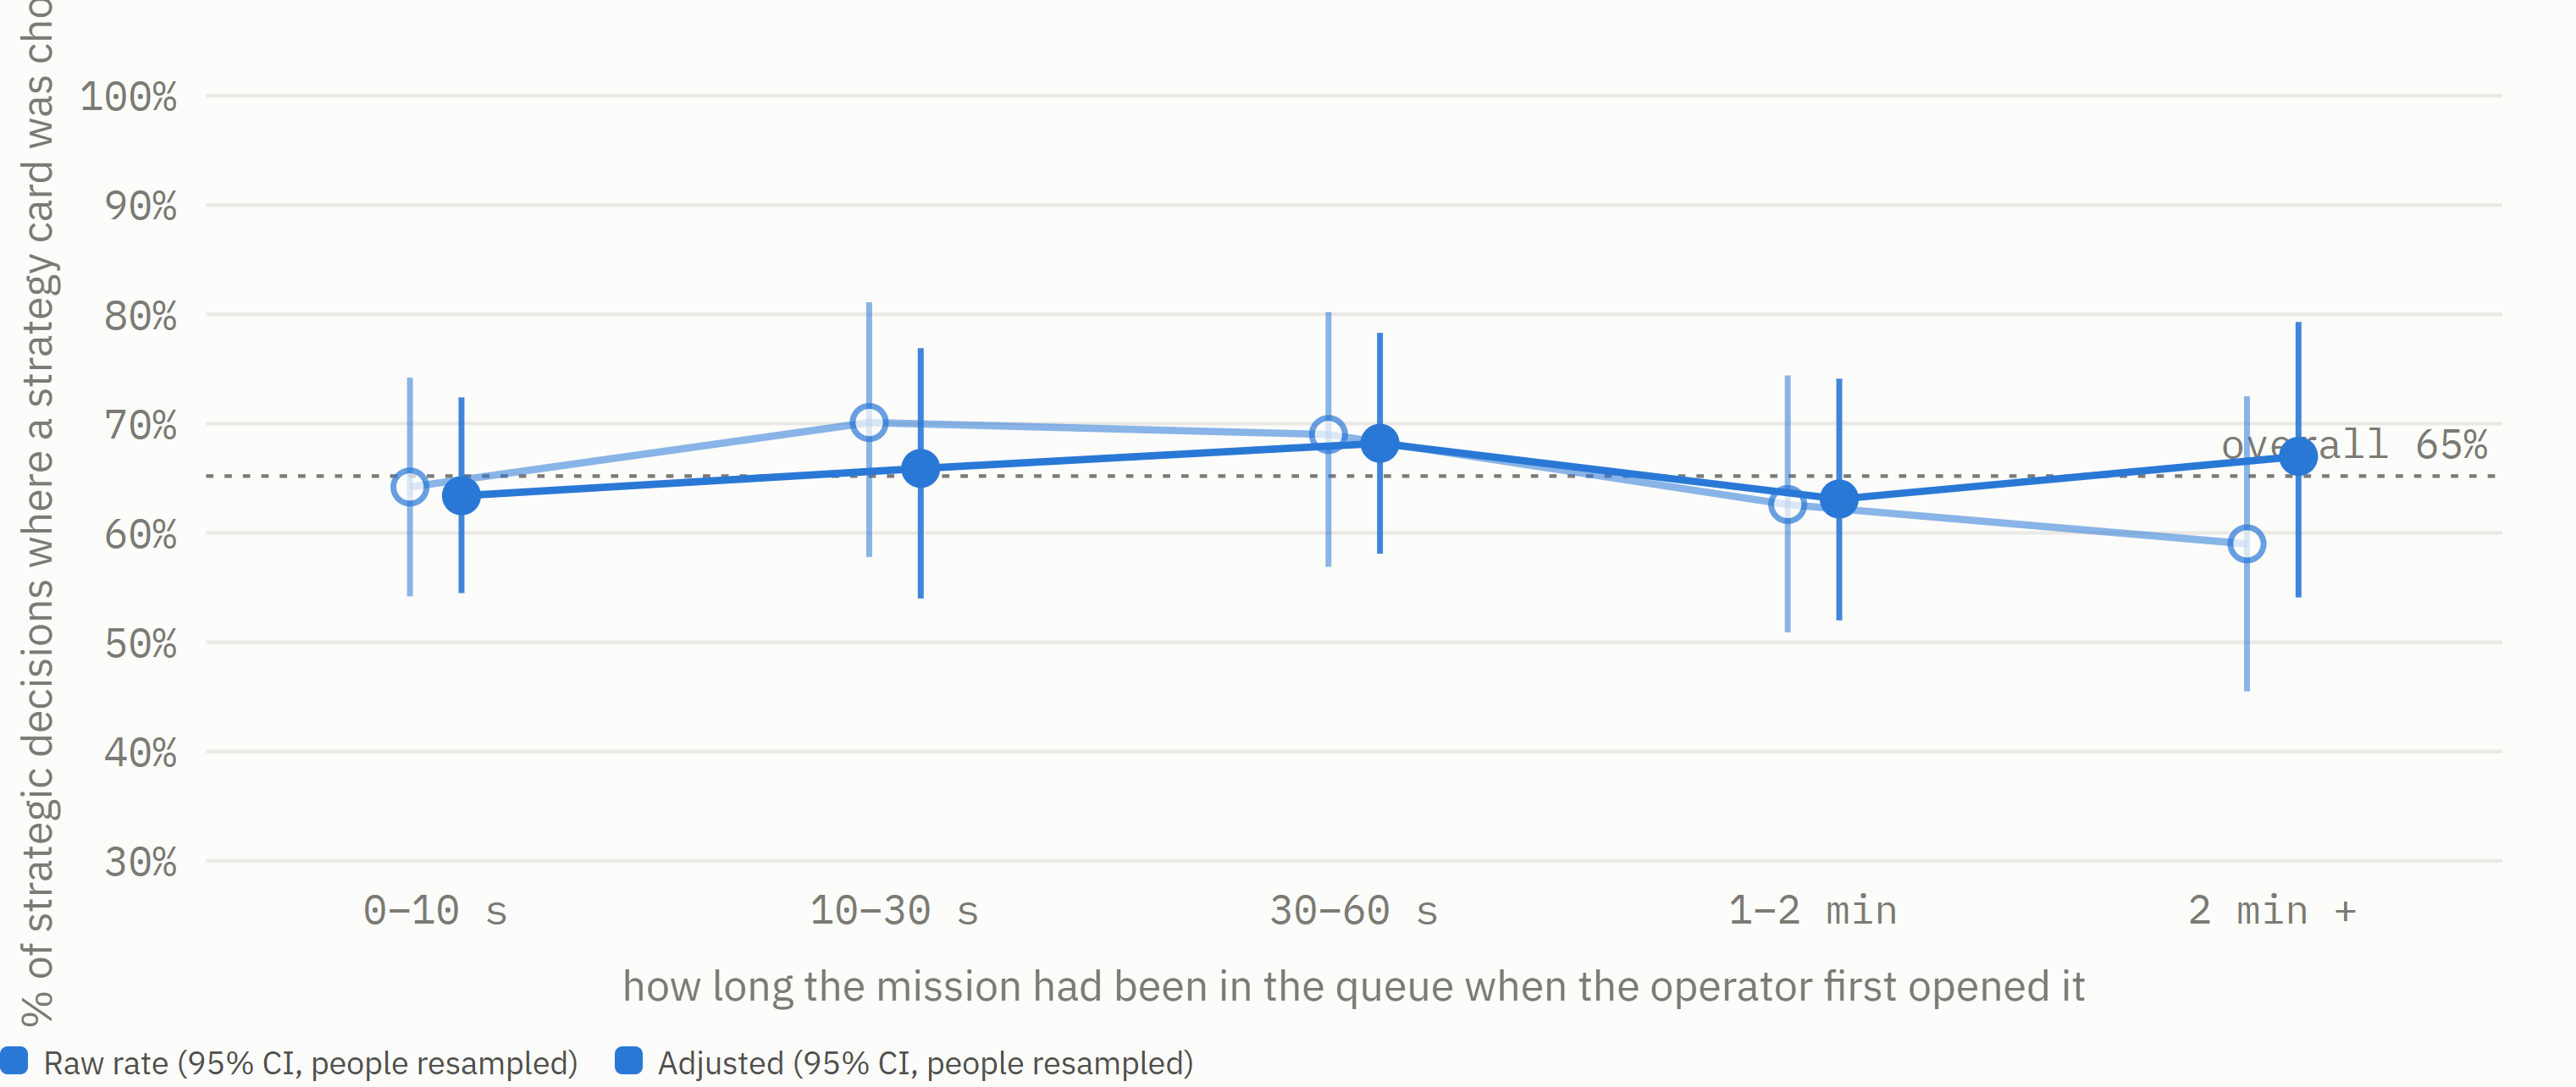
\includegraphics[width=\linewidth,height=0.24\textheight,keepaspectratio]{figs/results/f-workload__waited__strat.png}\par{\scriptsize Other view: Strategic tier: how long the mission had waited in the queue.}\end{minipage}\hfill
\begin{minipage}[t]{0.49\linewidth}\centering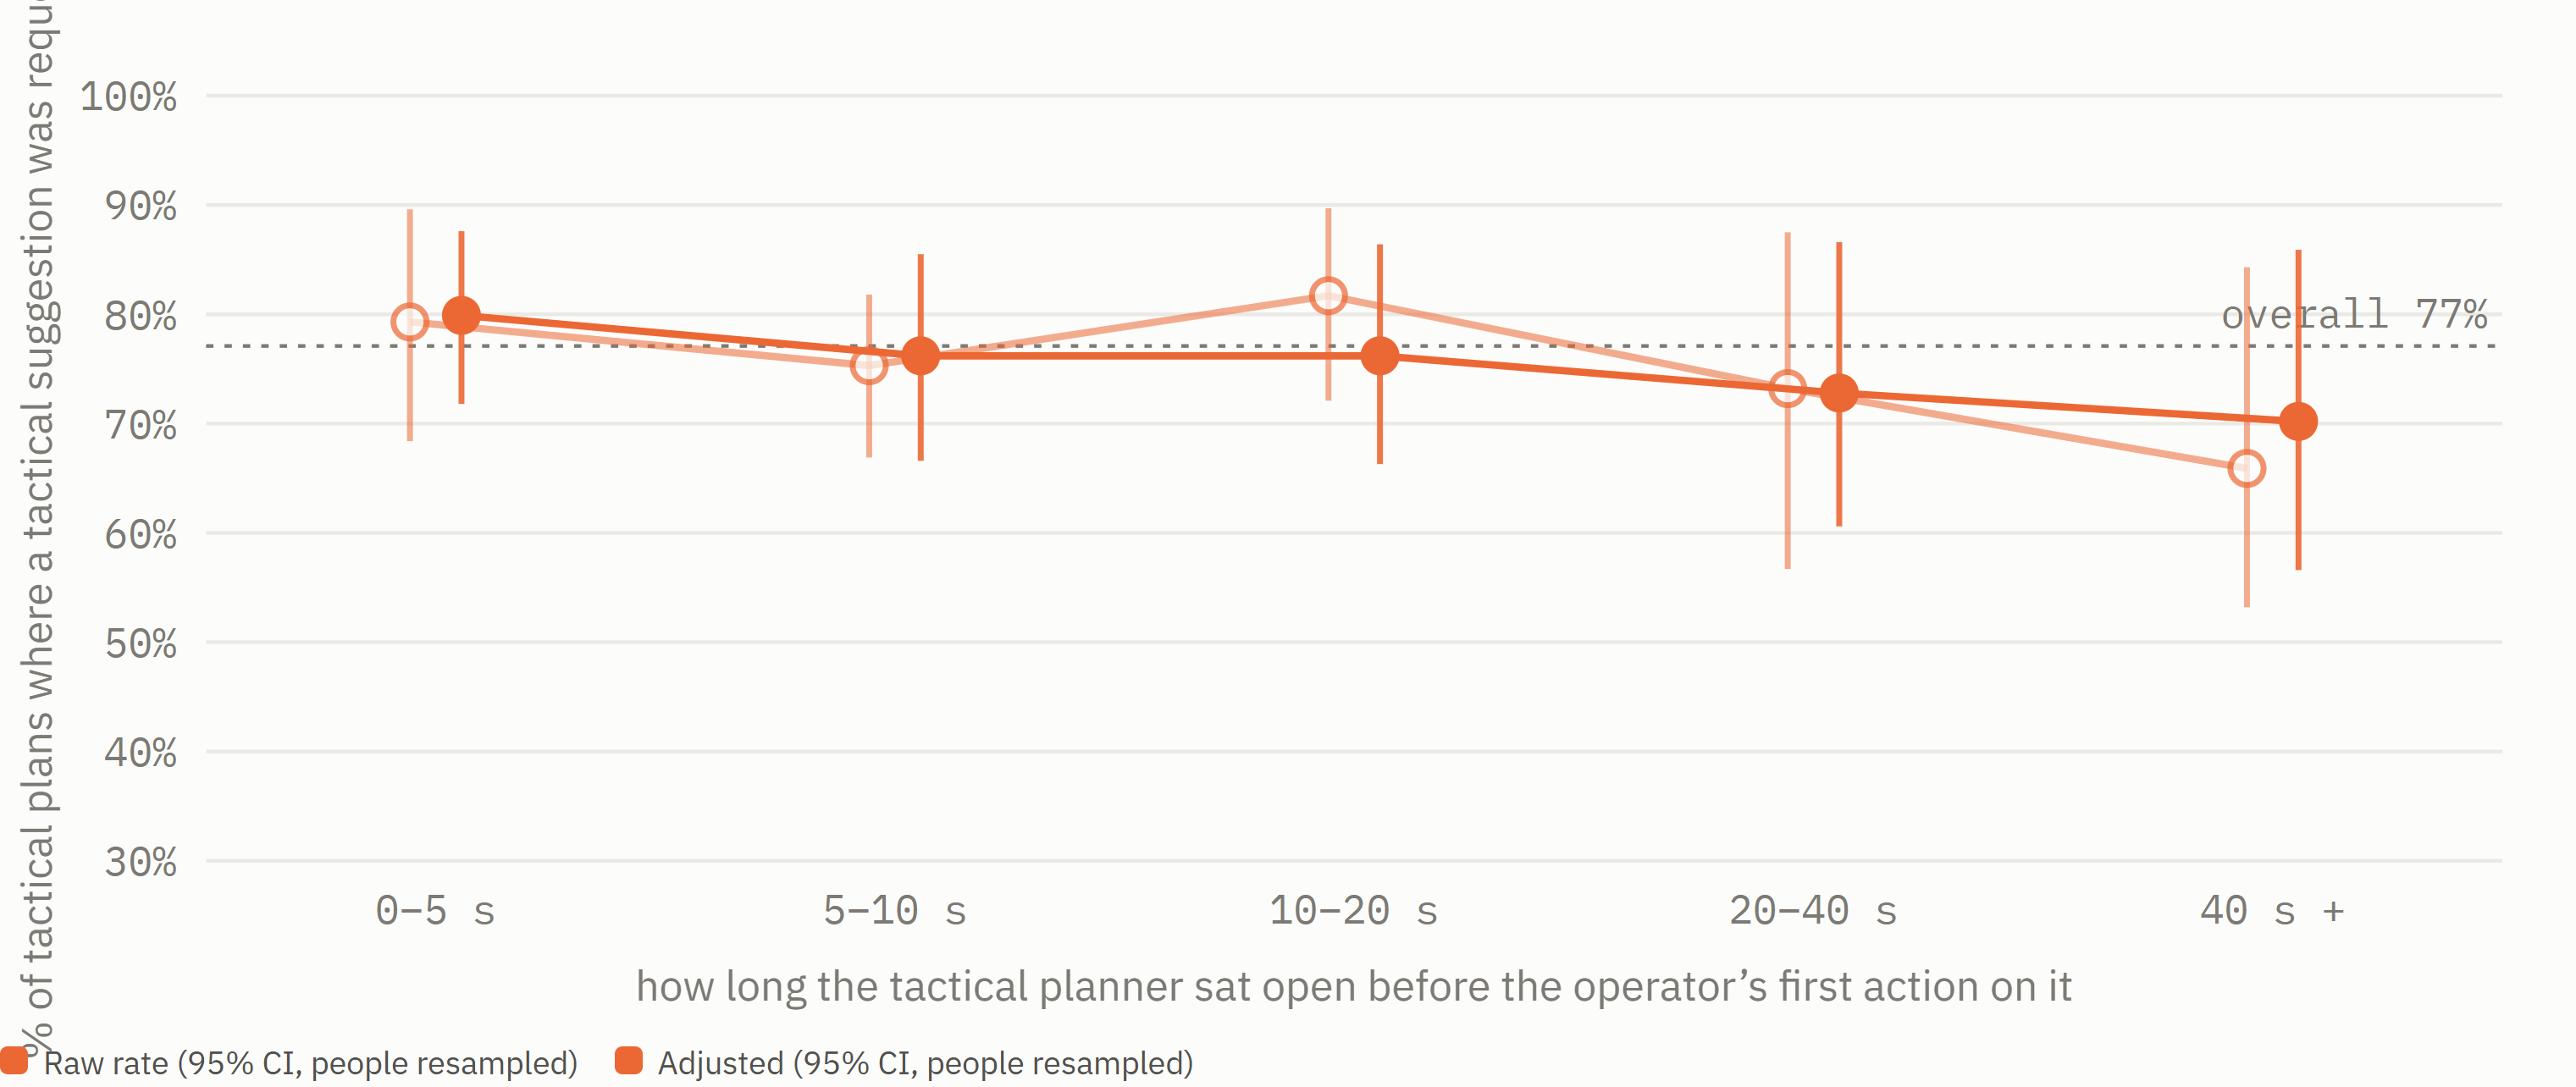
\includegraphics[width=\linewidth,height=0.24\textheight,keepaspectratio]{figs/results/f-workload__waited__tac.png}\par{\scriptsize Other view: Tactical tier: how long the plan had been left open.}\end{minipage}

\noindent Key numbers:\begin{itemize}[leftmargin=1.2em,itemsep=0pt]\footnotesize
\item Strategic (mission left in the queue): adjusted 63\% at 0--10 s, 66\% 10--30 s, 68\% 30--60 s, 63\% 1--2 min, 67\% at 2 min+ (n 173, 117, 100, 91, 83). Within person, odds $\times$1.10 per doubling of the wait [0.96, 1.28], p = .17; holding the queue fixed $\times$1.10, p = .19.
\item Tactical (plan left open): adjusted 80\% at 0--5 s, 76\% 5--10 s, 76\% 10--20 s, 73\% 20--40 s, 70\% at 40 s+ (n 270, 182, 93, 41, 44). Within person, odds $\times$0.80 per doubling [0.60, 1.06], p = .12; holding the queue fixed $\times$0.76, p = .10.
\end{itemize}
\end{options}

\clearpage

% ======== f-triage ========

\subsection{A long queue does not change what operators open}\label{sec:res:triage}

With a long queue, operators did not abandon order or pick smaller missions: compared with what was actually waiting, they kept the same priorities at any queue length.

% --- f-triage#order (pass 5: for the paper) ---

\phantomsection\label{sec:res:triage:order}\label{sec:res:triage:choice}
The share of decisions that opened the oldest waiting mission fell as the queue grew (59\% with one other waiting, about 30\% with five), but so did the chance of picking the oldest at random (50\% to 17\%); measured against chance, the pull towards the oldest stayed the same (Figure~\ref{fig:res:triage:order}). In a model of the choice among what was waiting, being the oldest roughly tripled a mission's chance of being opened, at short and long queues alike. Criticality pulls a little too: each category above the waiting missions' average raised the odds of being opened by about 1.45 (Section~\ref{sec:qual:new-jobs:queue-order}).

\begin{figure}[H]
\centering
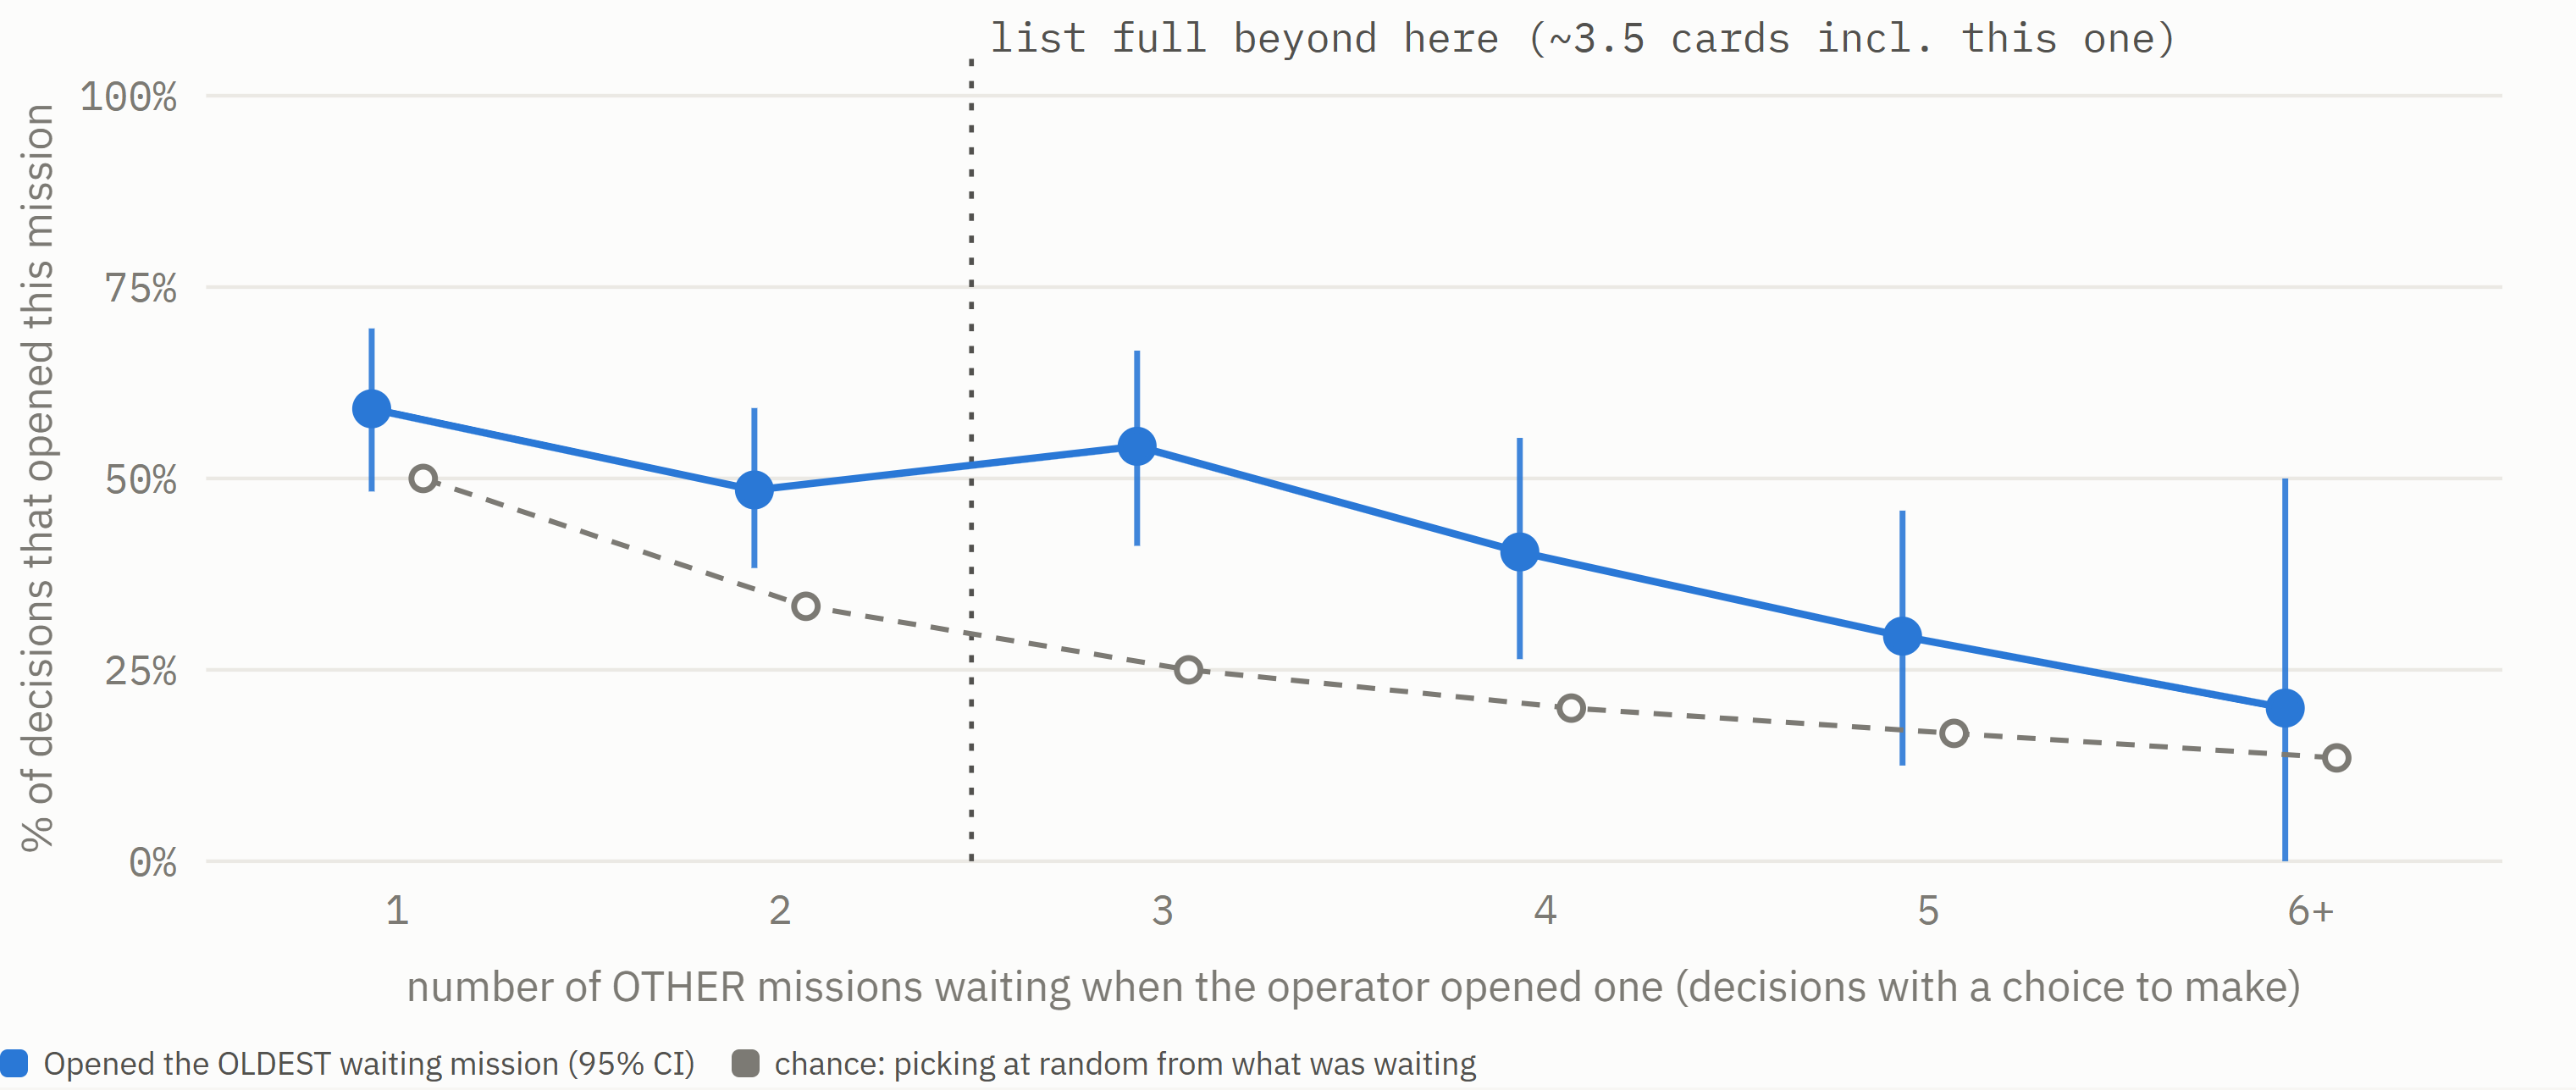
\includegraphics[width=\linewidth,height=0.50\textheight,keepaspectratio]{figs/results/f-triage__order__main.png}
\caption{\textbf{Operators open the oldest waiting mission well above chance at every queue length.}}
\label{fig:res:triage:order}
\end{figure}

\begin{options}
\optshead{Options for this finding}

\optsec{Order: still oldest-first well above chance} {\footnotesize [pass 5: for the paper]}

\noindent Key numbers:\begin{itemize}[leftmargin=1.2em,itemsep=0pt]\footnotesize
\item Opened the oldest: 59\% (1 other waiting; chance 50\%), 48\% (33\%), 54\% (25\%), 40\% (20\%), 29\% (17\%), 20\% (14\%).
\item Within person, the excess over chance does not shrink with depth: +2.4 points per extra mission [$-$1.0, +5.7], p = .16.
\end{itemize}

\optsec{What makes a waiting mission get opened, short vs long queues} {\footnotesize [pass 5: numbers only]}

\par\noindent \begin{minipage}[t]{0.49\linewidth}\centering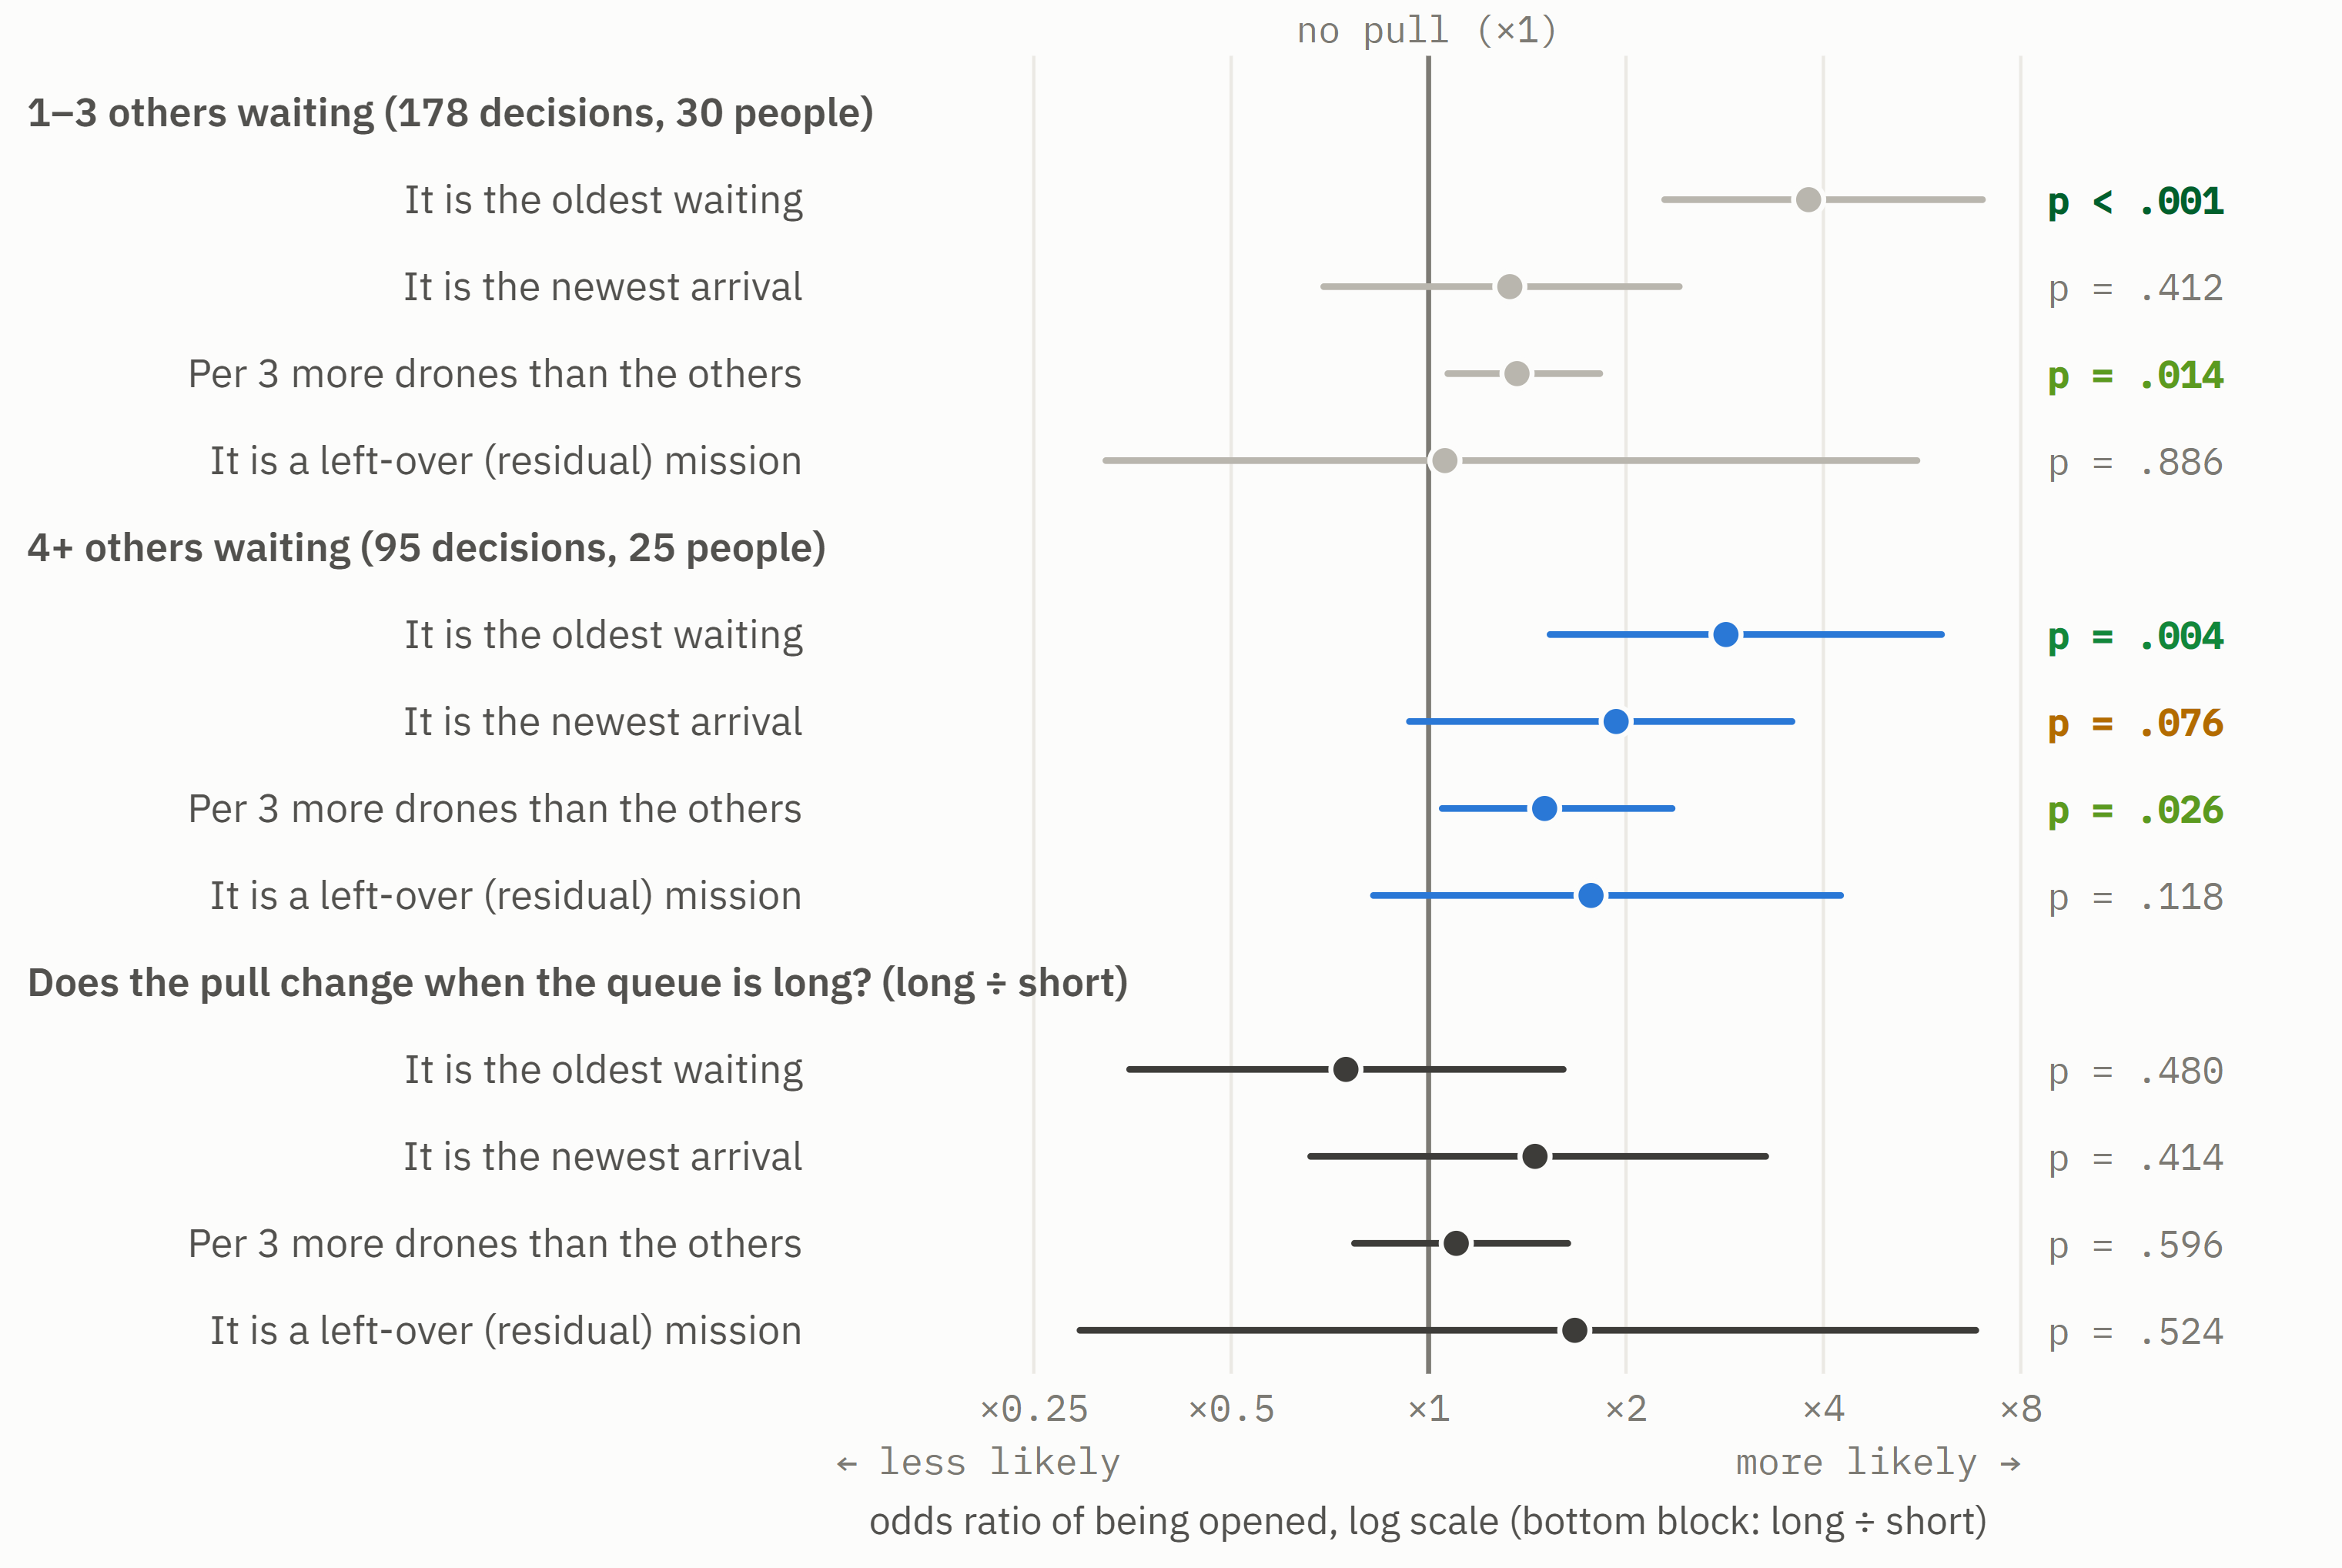
\includegraphics[width=\linewidth,height=0.24\textheight,keepaspectratio]{figs/results/f-triage__choice__sh.png}\par{\scriptsize Other view: Strategic Heavy games only.}\end{minipage}\hfill
\begin{minipage}[t]{0.49\linewidth}\centering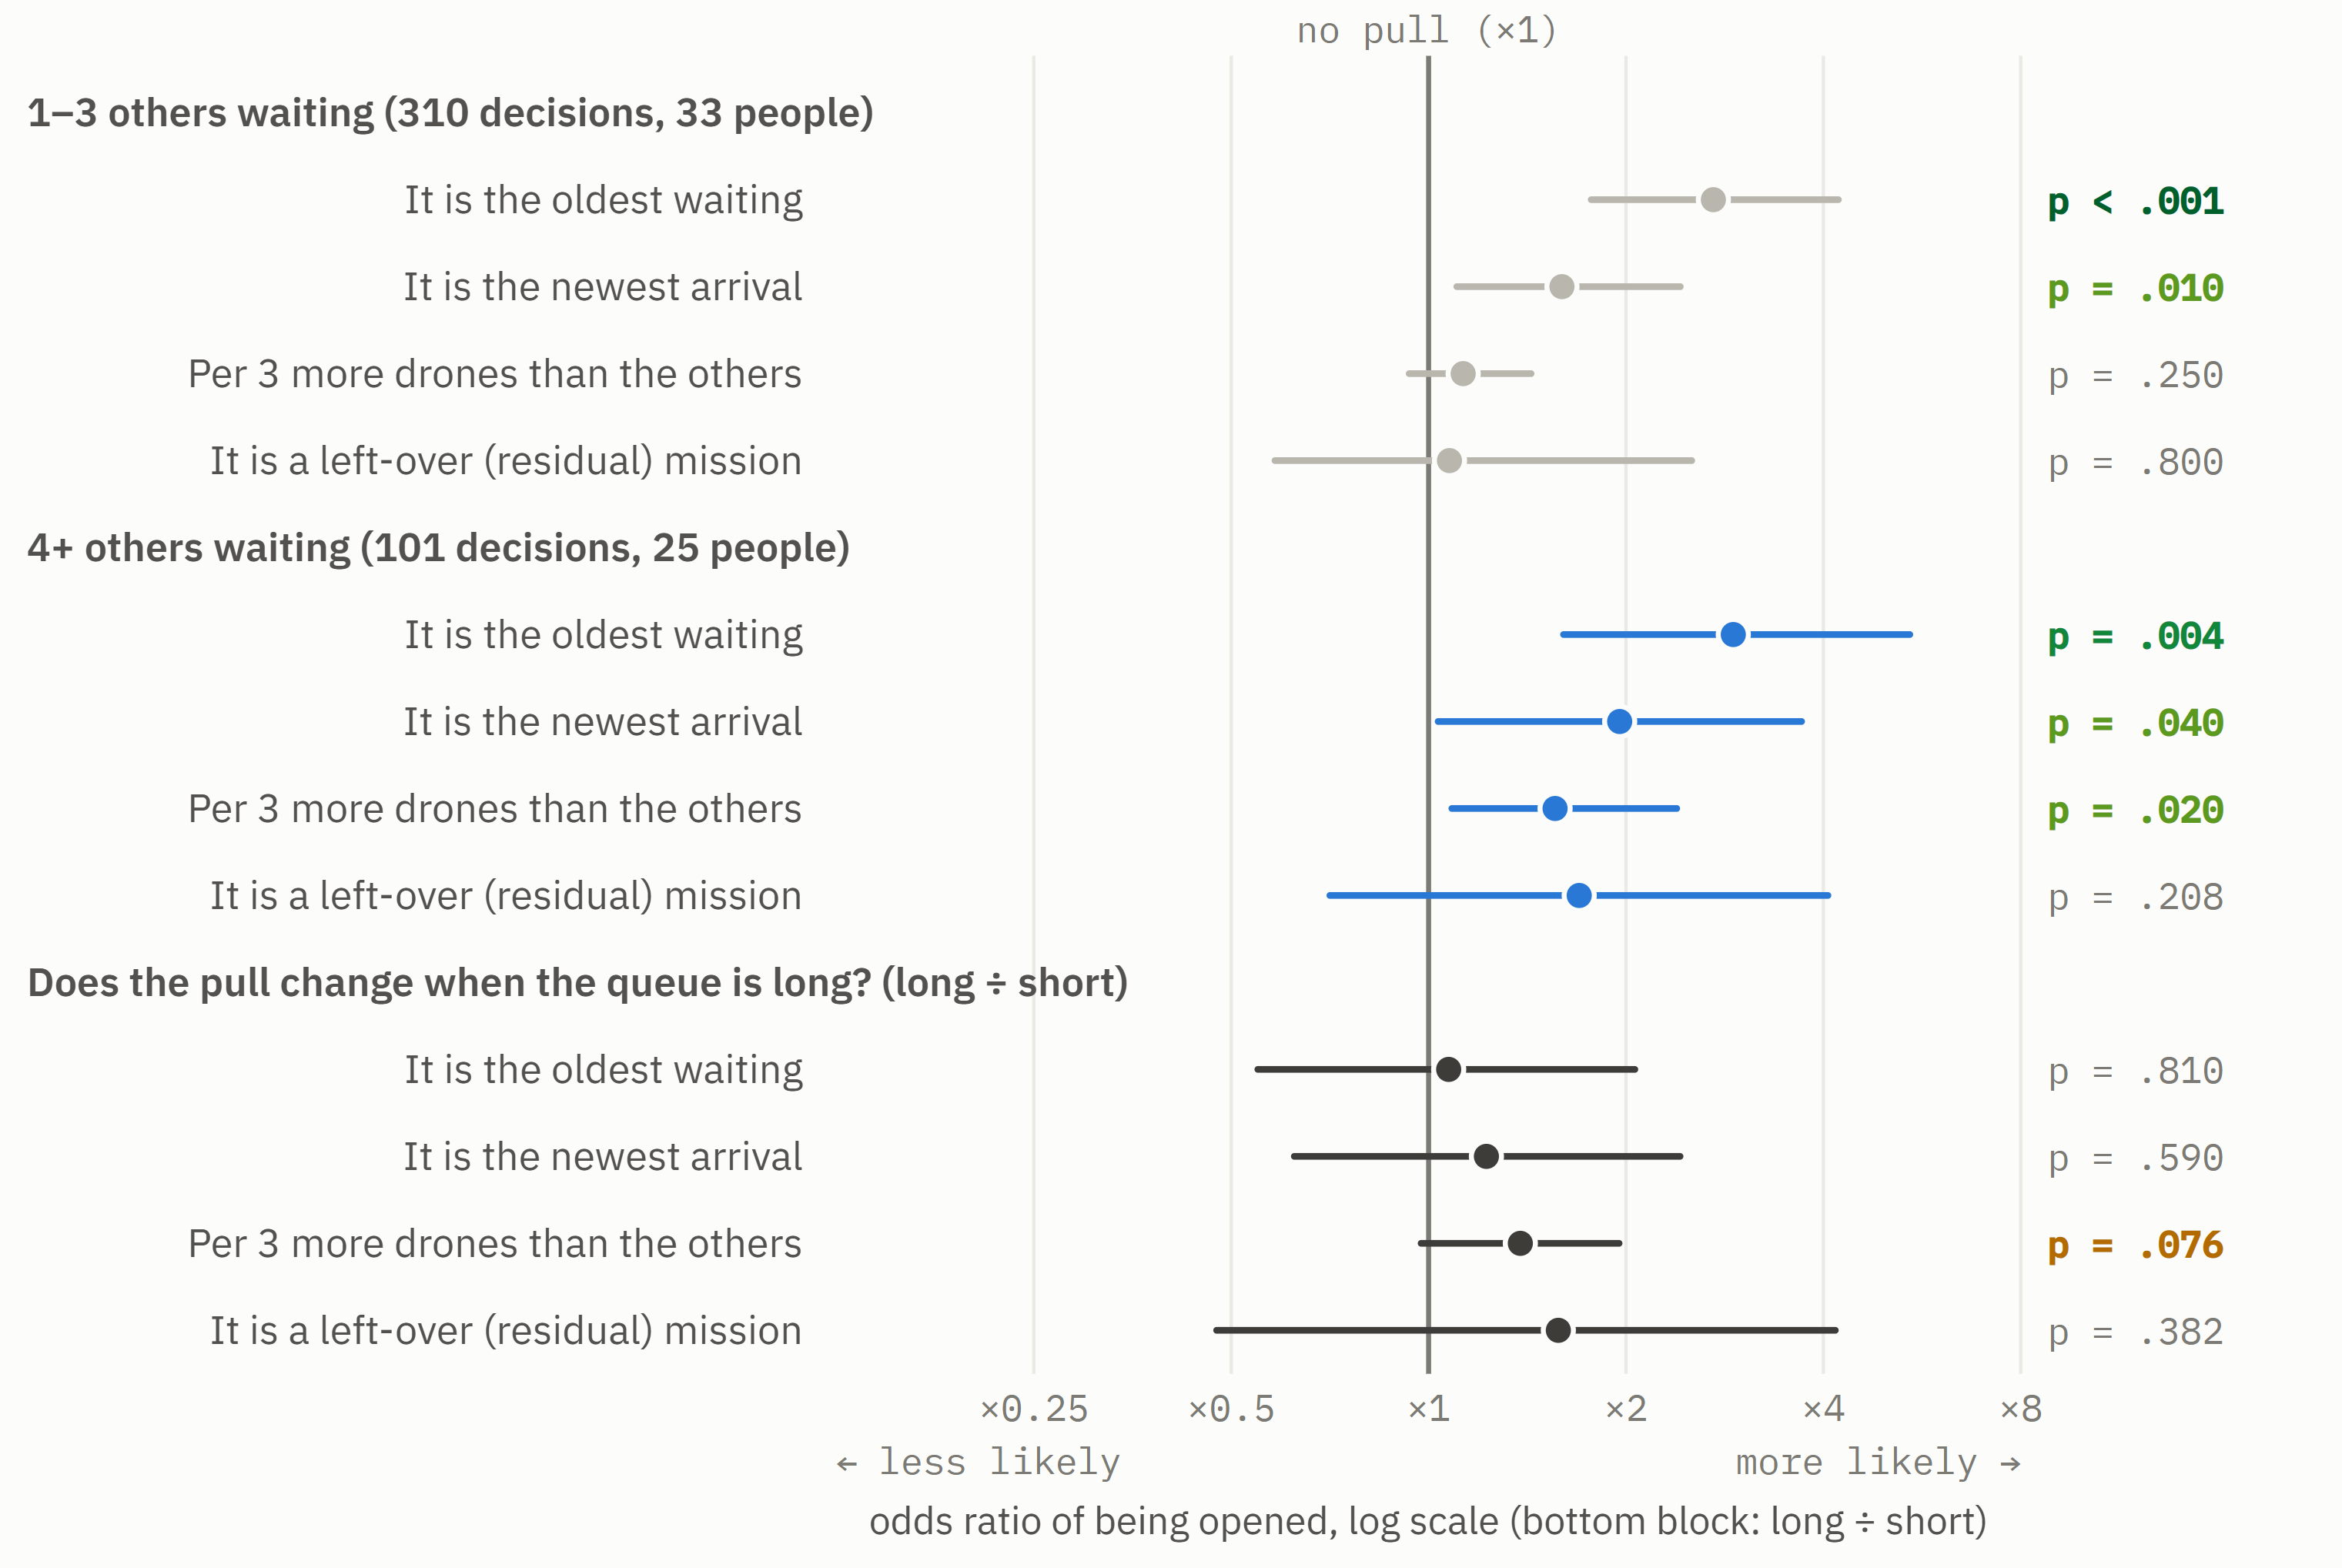
\includegraphics[width=\linewidth,height=0.24\textheight,keepaspectratio]{figs/results/f-triage__choice__all.png}\par{\scriptsize Other view: All four games.}\end{minipage}

\noindent Key numbers:\begin{itemize}[leftmargin=1.2em,itemsep=0pt]\footnotesize
\item Strategic Heavy games, short queues (178 decisions): oldest $\times$3.80 [2.29, 6.99], p < .001; newest $\times$1.33 [0.69, 2.41], p = .41; +3 drones $\times$1.36 [1.07, 1.82], p = .014; residual $\times$1.06, p = .89
\item Strategic Heavy games, long queues (95 decisions): oldest $\times$2.84 [1.53, 6.06], p = .004; newest $\times$1.93 [0.94, 3.58], p = .076; +3 drones $\times$1.50 [1.05, 2.35], p = .026; residual $\times$1.77, p = .12
\item Long $\div$ short, Strategic Heavy games: oldest $\times$0.75 [0.35, 1.60], p = .48; newest $\times$1.45, p = .41; size $\times$1.10, p = .60; residual $\times$1.67, p = .52 (none differs)
\item All four games: oldest $\times$2.72 (short) and $\times$2.92 (long), both p $\leq$ .004; newest $\times$1.60, p = .010 and $\times$1.96, p = .040; size $\times$1.13, p = .25 and $\times$1.56, p = .020; long $\div$ short for size $\times$1.38 [0.97, 1.95], p = .076, all others p $\geq$ .38
\end{itemize}
\end{options}

\clearpage

% ======== f-flaw-odd ========

\subsection{The illogical strategy card, and who stopped choosing the cards}\label{sec:res:flaw-odd}

The Conservative strategy card sometimes added a drone type the mission did not use (22\% of decisions, nearly all on one-type missions), and all 33 people met it, usually on their first or second decision. The 15 who later said they noticed it chose strategy cards less afterwards, and on the flawed one-type missions they learned to skip the card. But the dip in their use is not tied to the illogical card itself: it appears early in the first session whether or not they had met that card yet, and in the same stretch the people who never mentioned it chose the cards more. Our best reading is that ``noticed'' marks people who scrutinise the cards, and the dip is that scrutiny at the first busy stretch of the study. The evidence is suggestive (15 against 18 people).

% --- f-flaw-odd#event (pass 5: for the paper) ---

\phantomsection\label{sec:res:flaw-odd:event}
Lined up on each person's first illogical card (Figure~\ref{fig:res:flaw-odd:event:pairs}), noticers went from choosing a strategy card on 76\% of decisions before it to 43--52\% for their next ten decisions, recovering to 67--68\% only from the eleventh on; people who never mentioned it stayed at 67--75\% throughout. On three-type missions, which never carry the flaw, noticers dipped for a short stretch and recovered (74\% before, 43\% for the next two decisions, then 59--63\% and 75\%). Many first met the card with puzzlement rather than a verdict: ``Oh, this just sends a bunch of extra of these even though it doesn't need it?'' (P19); ``But in conservative, you don't need camera or lifters, yet it adds it as reserve. Even for tasks it doesn't do. That doesn't make sense.'' (P13).

\begin{figure}[H]
\centering
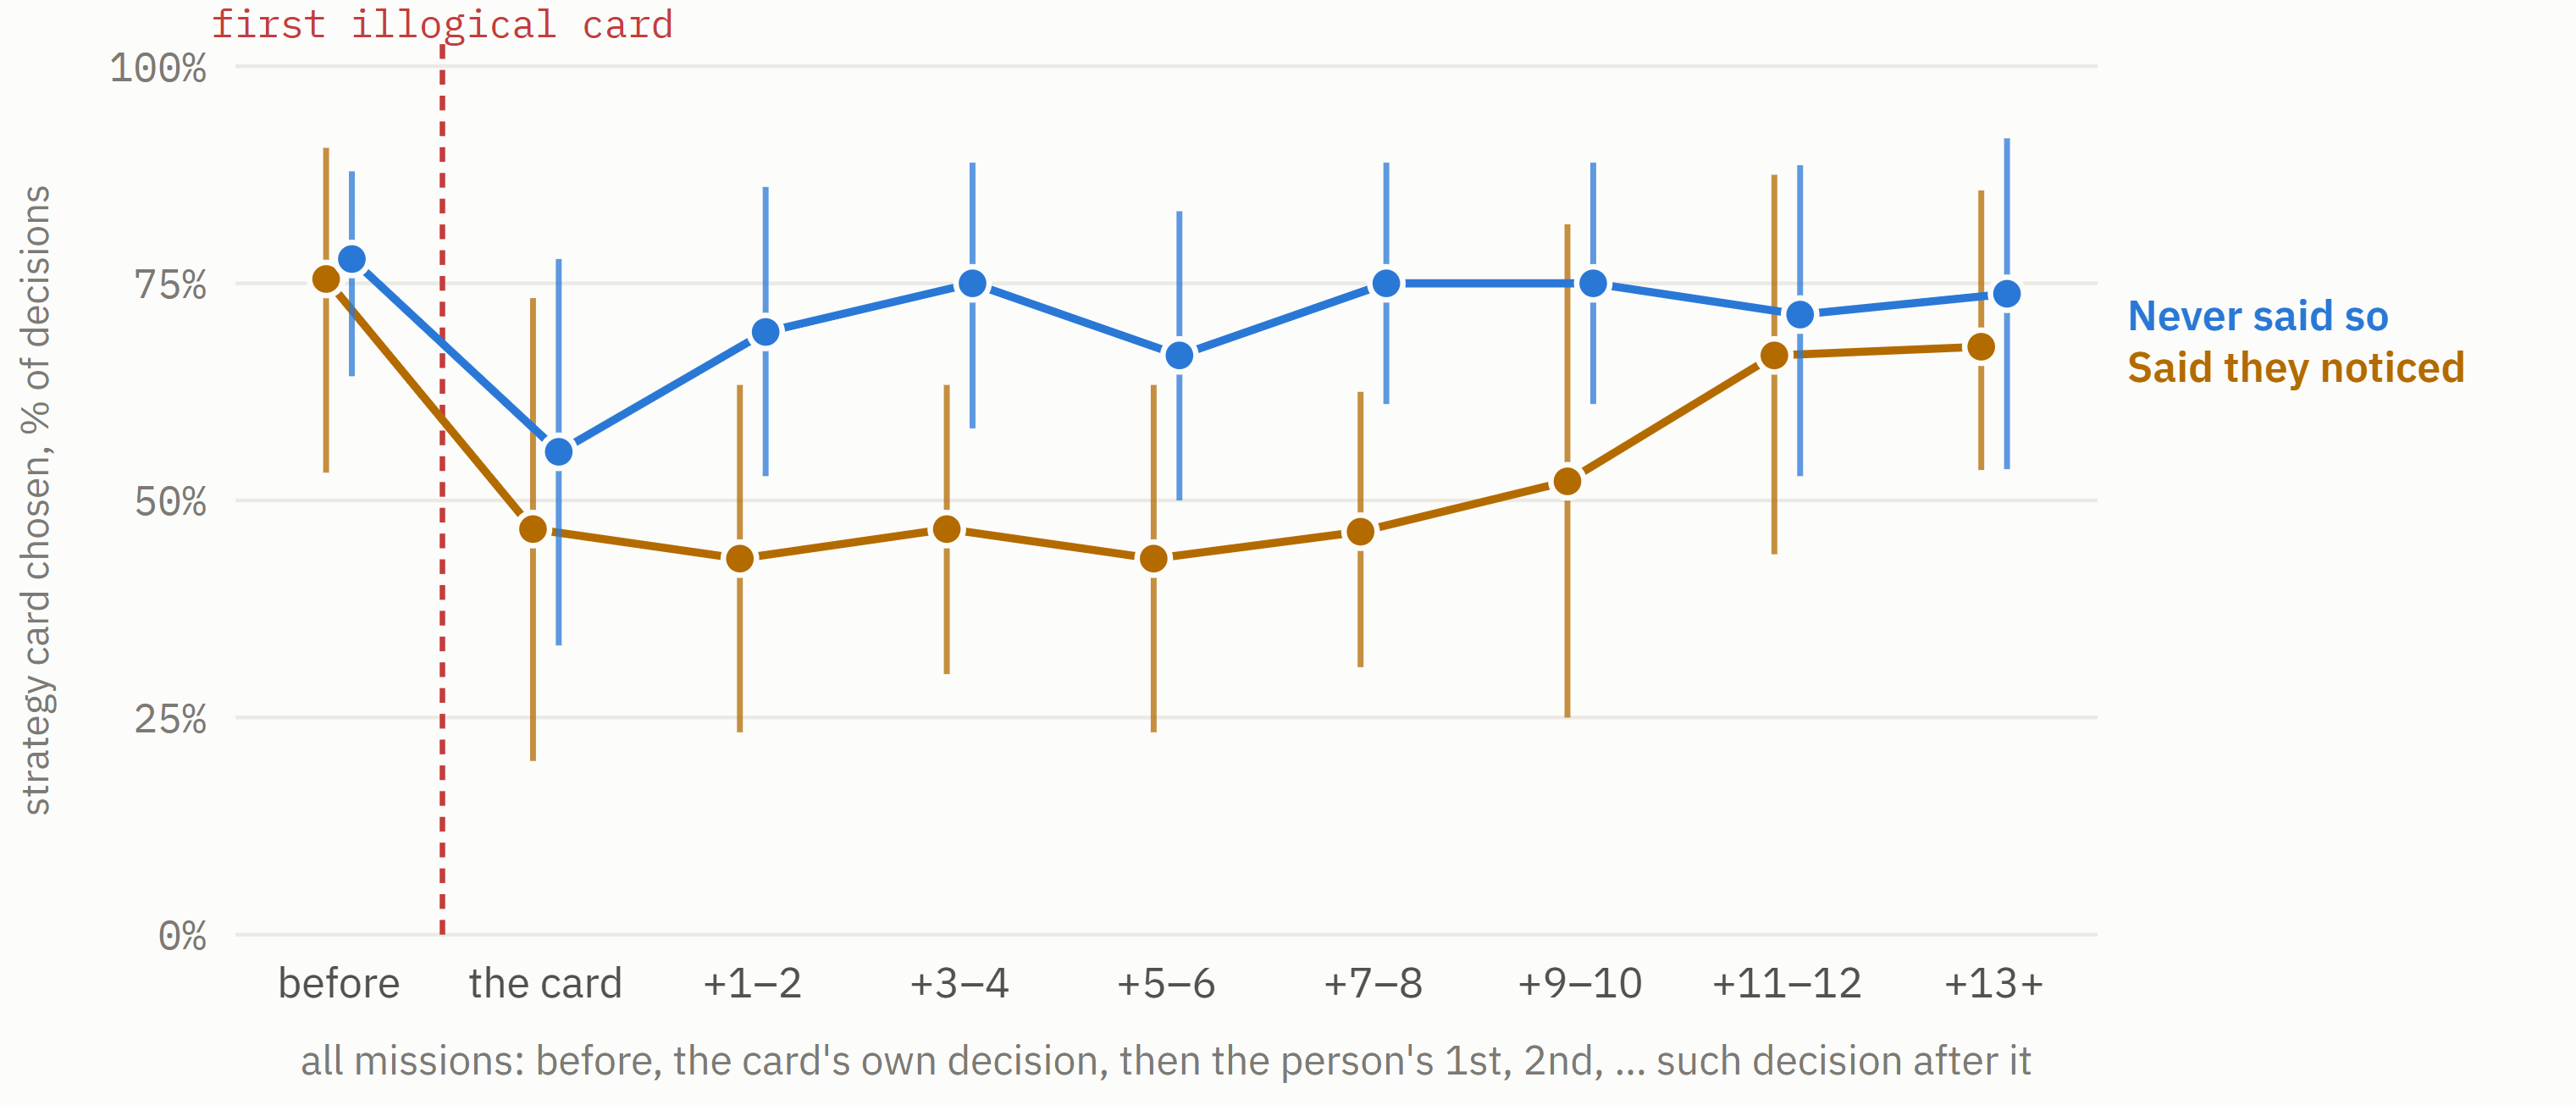
\includegraphics[width=\linewidth,height=0.50\textheight,keepaspectratio]{figs/results/f-flaw-odd__event__pairs.png}
\caption{\textbf{After the first illogical strategy card, those who later said they noticed it choose the cards less for about ten decisions.} Share of decisions where a strategy card was chosen, by decision number after the first illogical card, in pairs.}
\label{fig:res:flaw-odd:event}
\label{fig:res:flaw-odd:event:pairs}
\end{figure}

% --- f-flaw-odd#over-time (pass 5: for the paper) ---

\phantomsection\label{sec:res:flaw-odd:over-time}
Not lined up on the card but placed by the minute of the session (Figure~\ref{fig:res:flaw-odd:over-time}), the dip is still there. In session 1 noticers started at 86\% in the first minute, fell to 38--50\% over minutes one to four and came back to 73\%, while the others rose over the same minutes (65\% to 88\%). Pooled over everyone the line stays at 61--77\%, because the two groups move in opposite directions. Several kept using the cards anyway for the time they saved: ``I think it's less reliable than before, but I still use its suggestion, and that's the case. Yeah, because at least it saves time.'' (P28).

\begin{figure}[H]
\centering
\begin{subfigure}[t]{\linewidth}
\centering
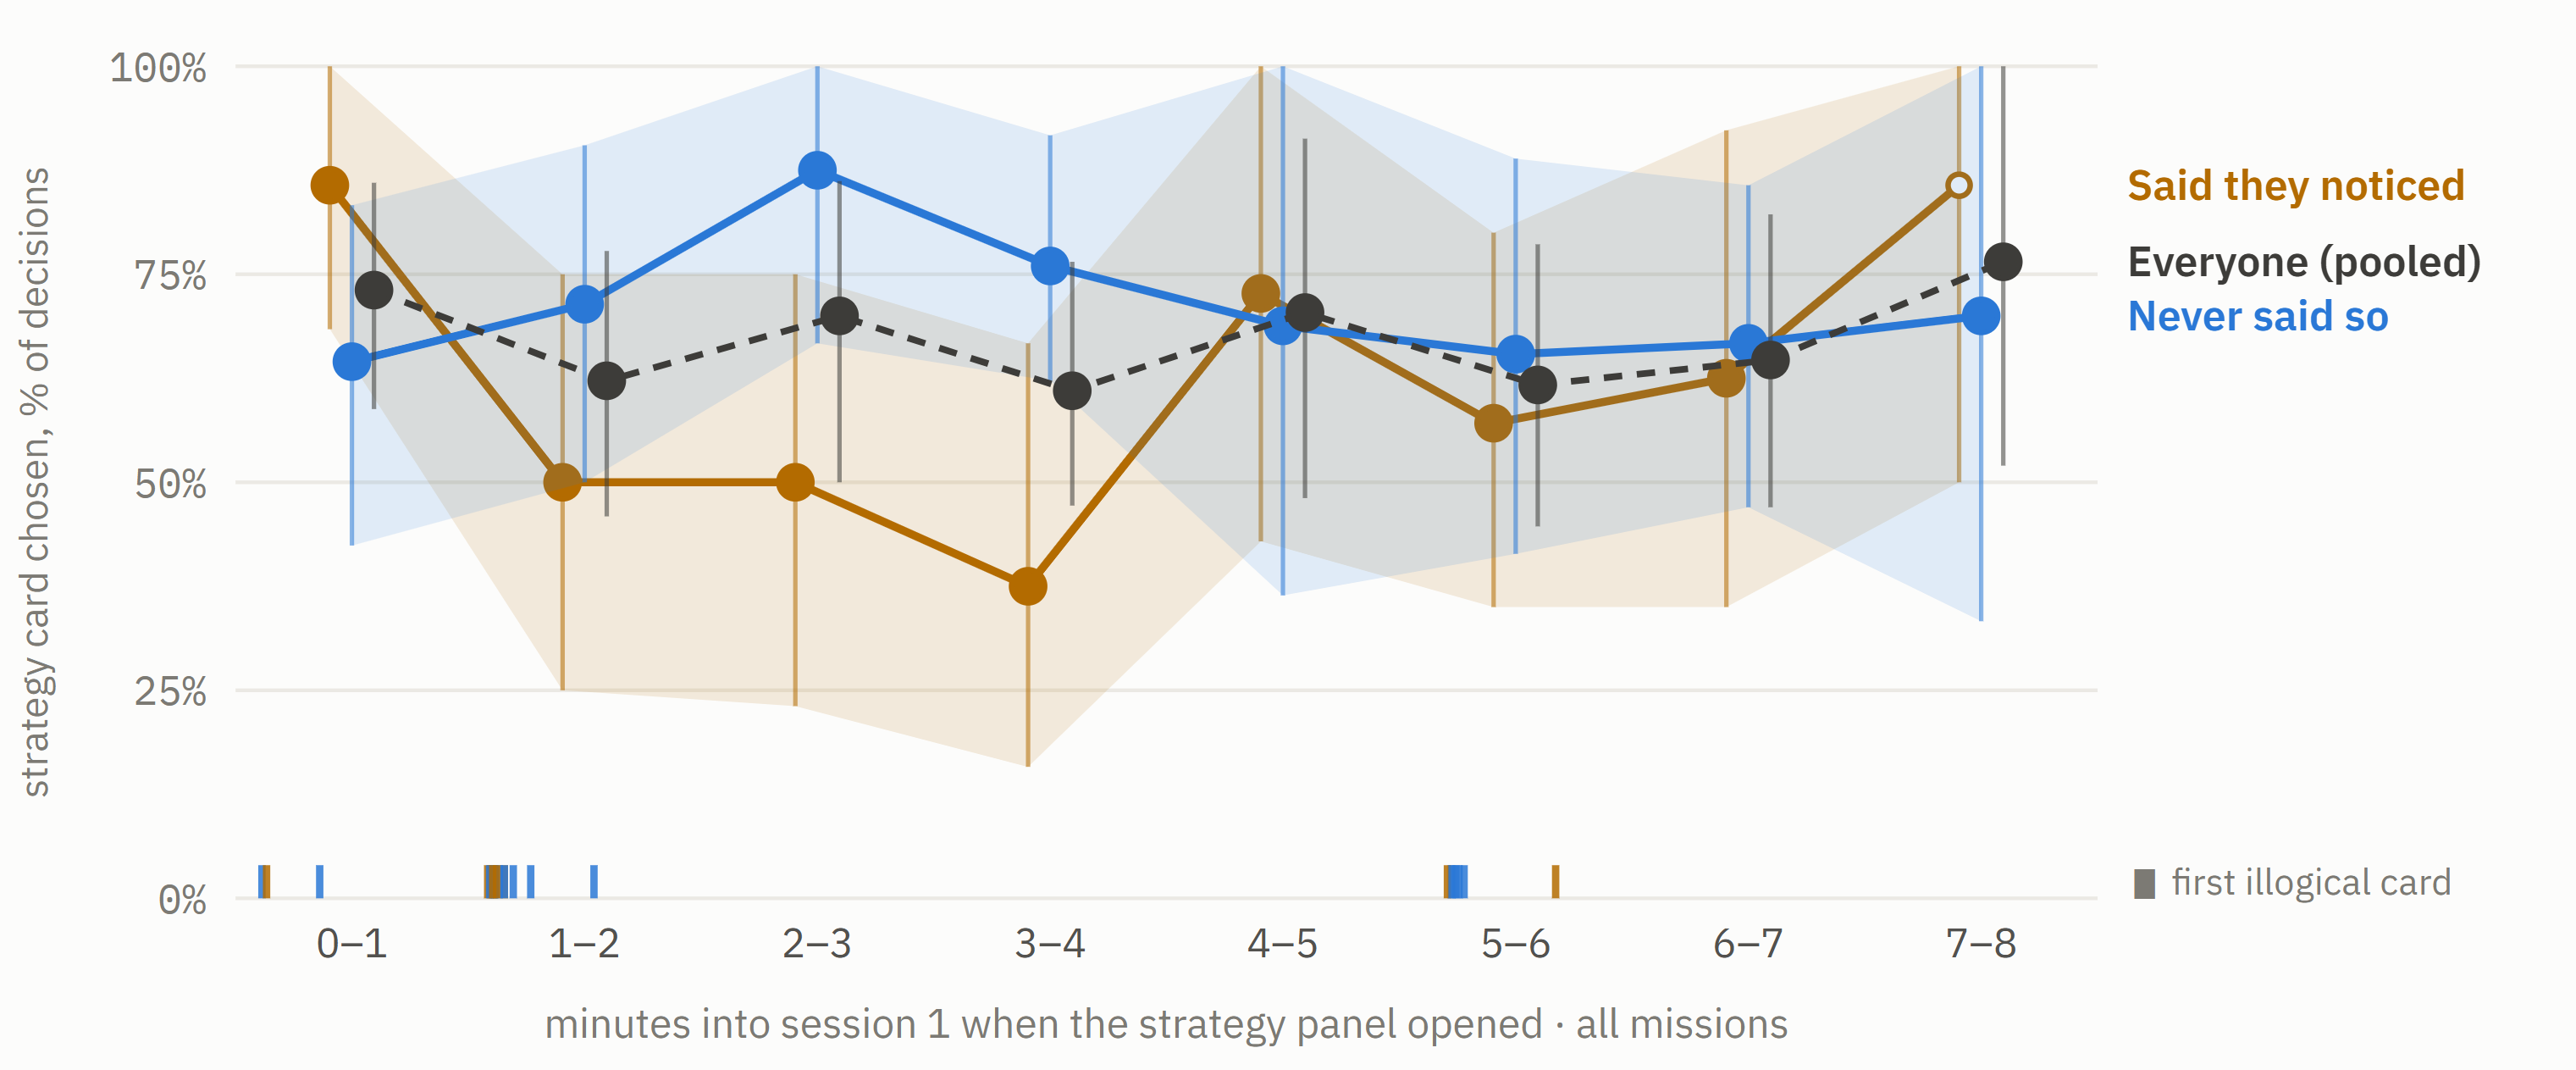
\includegraphics[width=\linewidth,height=0.21\textheight,keepaspectratio]{figs/results/f-flaw-odd__over-time__s1.png}
\caption{Session 1: each group and everyone.}
\label{fig:res:flaw-odd:over-time:s1}
\end{subfigure}
\par\smallskip
\begin{subfigure}[t]{\linewidth}
\centering
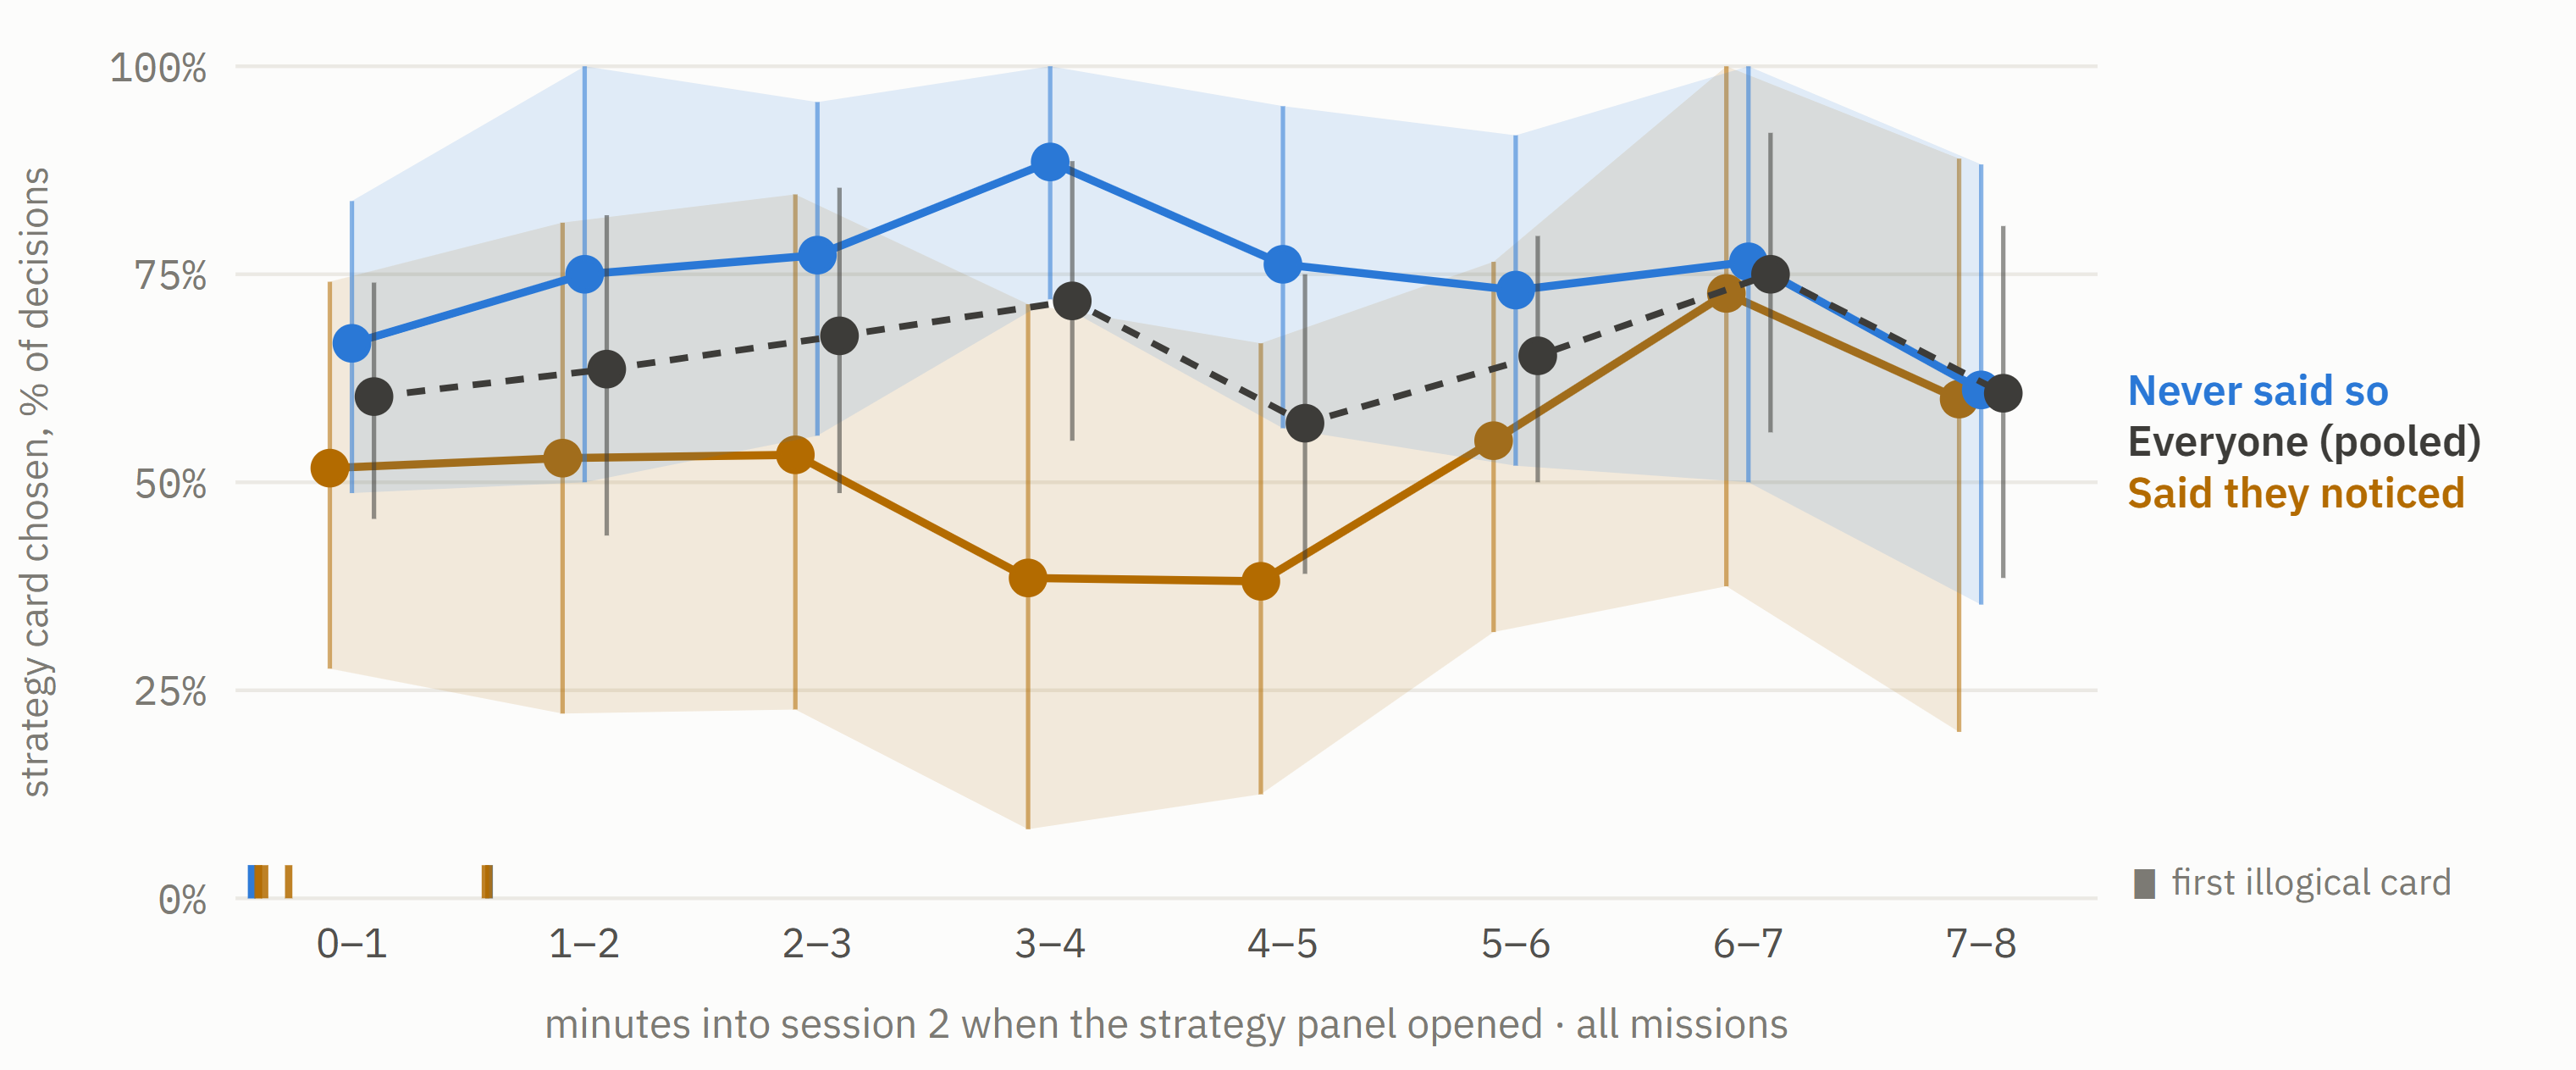
\includegraphics[width=\linewidth,height=0.21\textheight,keepaspectratio]{figs/results/f-flaw-odd__over-time__s2.png}
\caption{Session 2: each group and everyone.}
\label{fig:res:flaw-odd:over-time:s2}
\end{subfigure}
\par\smallskip
\caption{\textbf{Early in the session the two groups move in opposite directions, so pooling them hides the dip.} Share of strategic decisions with a strategy card chosen, by minute of the session, for noticers, the others and everyone (dashed): (a) session 1, (b) session 2.}
\label{fig:res:flaw-odd:over-time}
\end{figure}

% --- f-flaw-odd#by-index (pass 5: for the paper) ---

\phantomsection\label{sec:res:flaw-odd:by-index}
Counted simply by decision number (Figure~\ref{fig:res:flaw-odd:by-index:groups}), noticers chose a strategy card on 80\% of their first decisions of session 1 and 46--50\% of decisions three to five, then 83\% at the sixth, while the others rose to 89--94\% in the same stretch. People who played the Tactical Heavy game first had not yet met an illogical card by decisions three to five (95\% of those decisions came before it), and their noticers dipped just as much ($-21$ points per person, against $-32$ for those who had met it; $p = .79$). Noticers recovered within session 1 ($+24$ points per person) and started session 2 lower again, but so did the others, so a weaker carry-over for noticers cannot be shown (difference at the break $-6$ points [$-32$, $+20$]).

\begin{figure}[H]
\centering
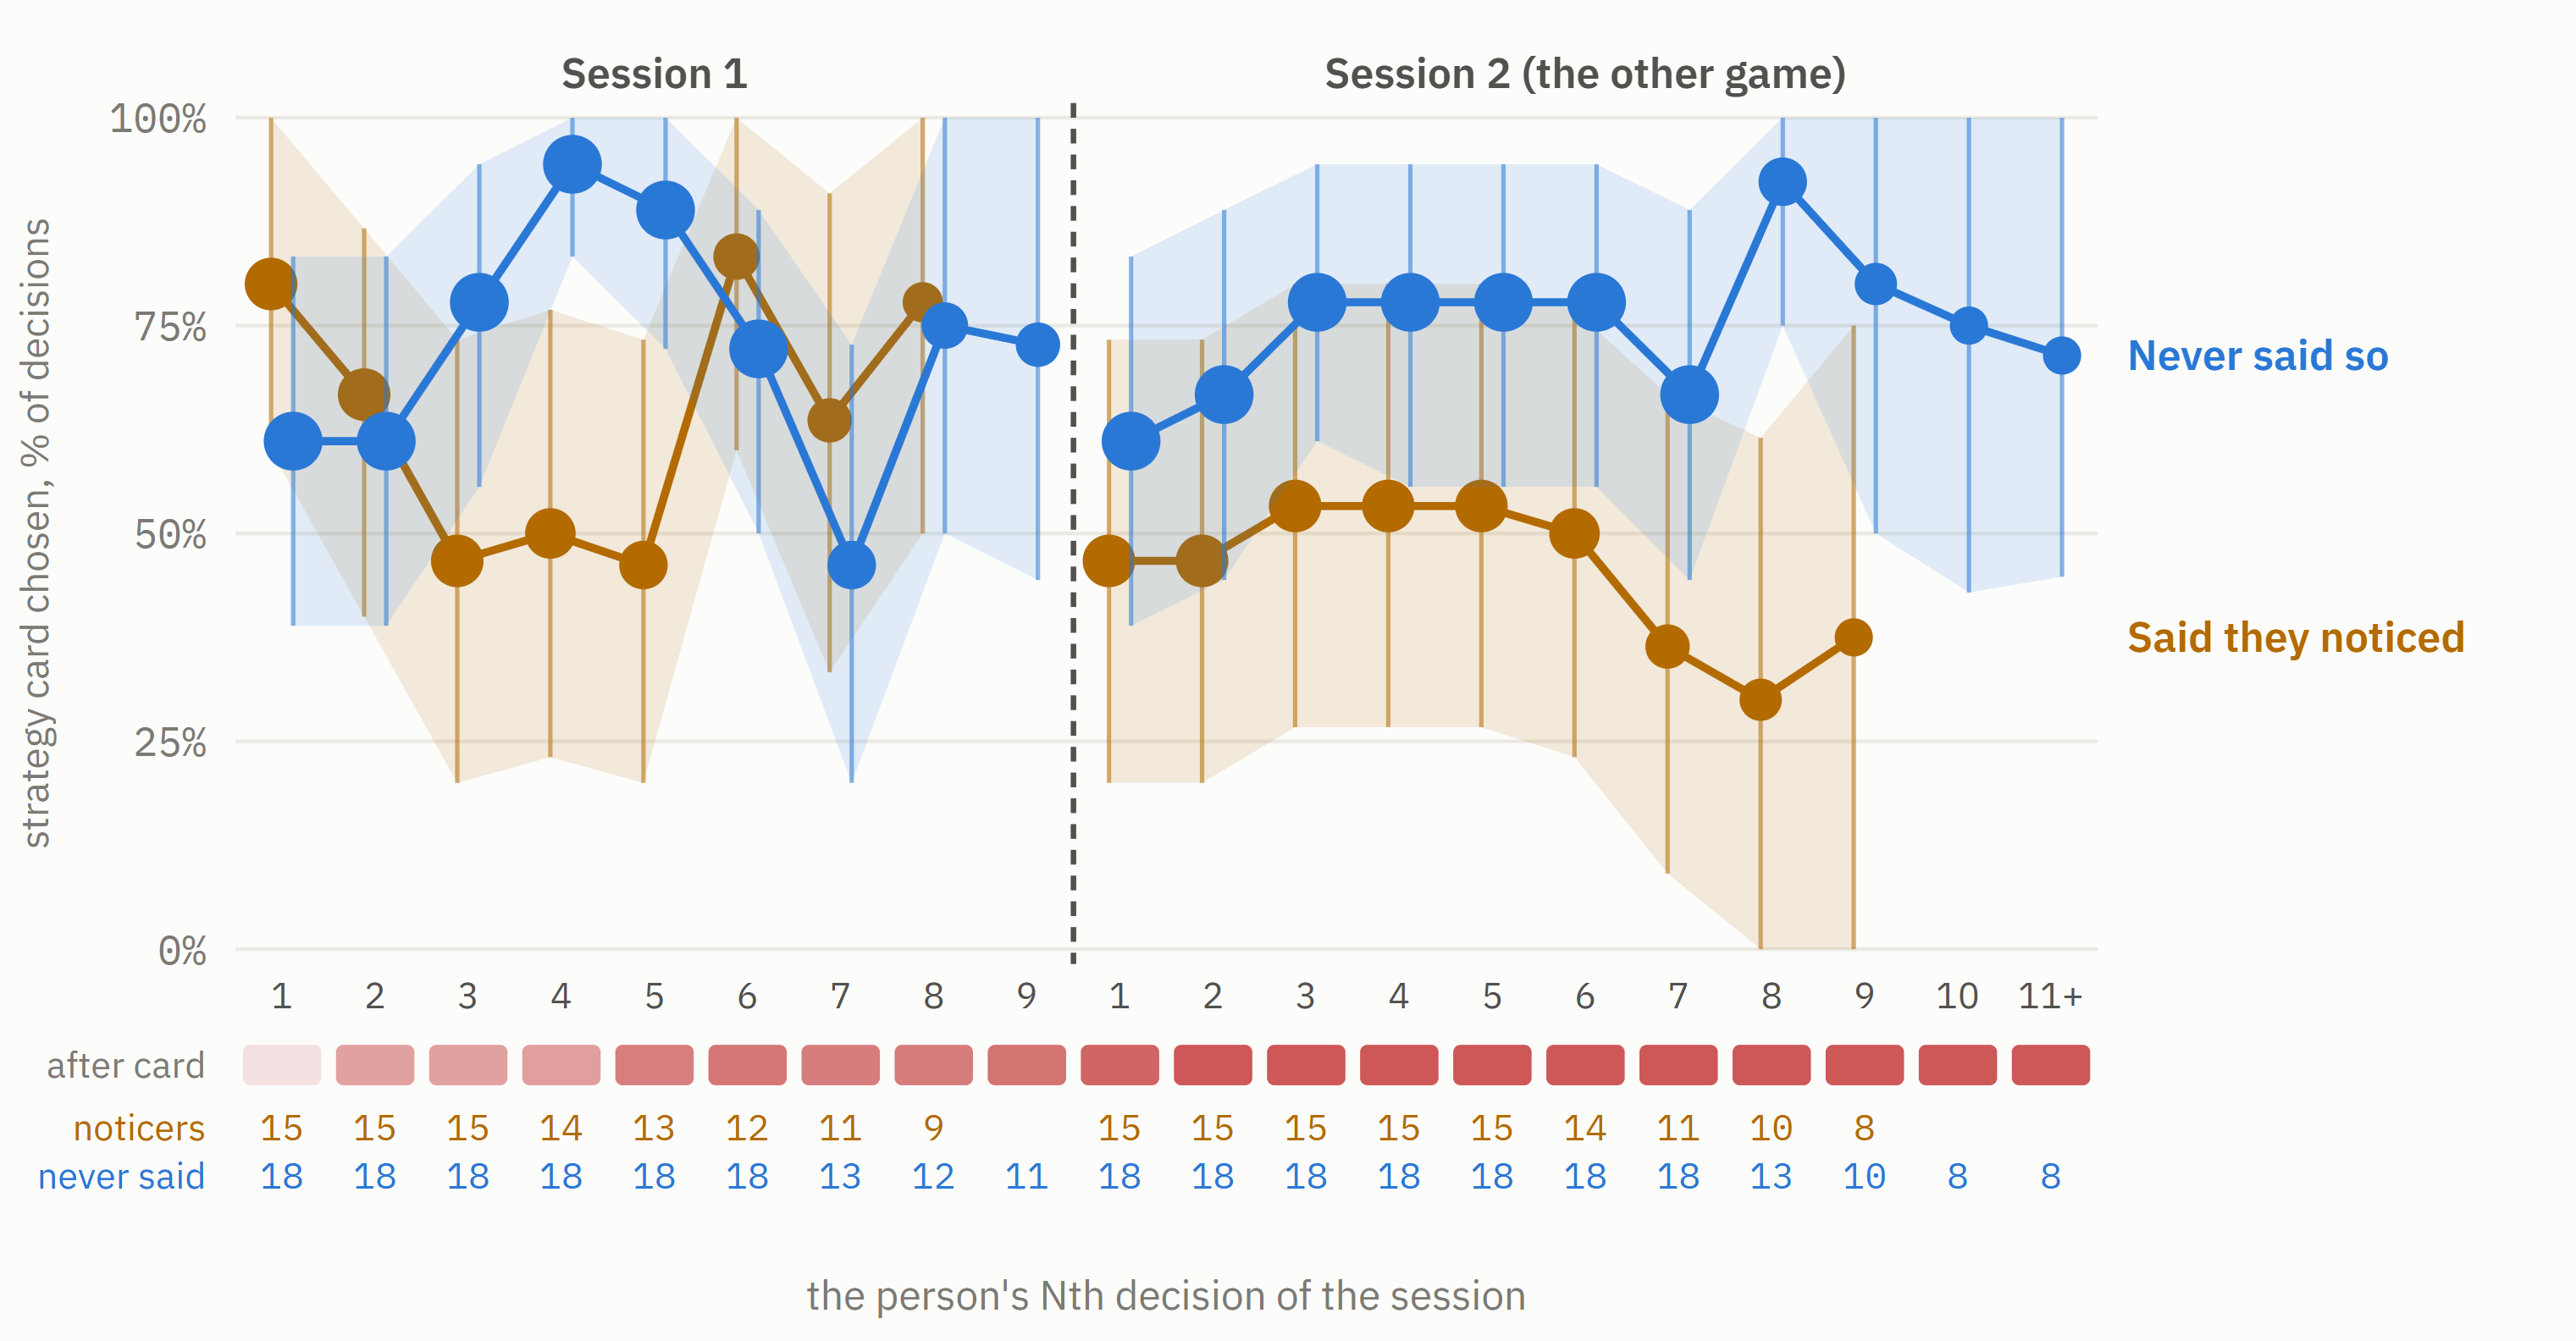
\includegraphics[width=\linewidth,height=0.50\textheight,keepaspectratio]{figs/results/f-flaw-odd__by-index__groups.png}
\caption{\textbf{Counted by decision number, the noticers' dip comes before most of them have met an illogical card.} Share of decisions with a strategy card chosen, session 1 then session 2.}
\label{fig:res:flaw-odd:by-index}
\label{fig:res:flaw-odd:by-index:groups}
\end{figure}

% --- f-flaw-odd#spoken (pass 5: for the paper) ---

\phantomsection\label{sec:res:flaw-odd:spoken}\label{sec:res:flaw-odd:refusal}
Lining people up instead on the moment they said aloud that a card was wrong gives the same direction (Figure~\ref{fig:res:flaw-odd:spoken:strict}). Seven people made such a remark; they went from choosing a strategy card on 80\% of decisions before it to 49\% after (adjusted $-21$ points, $p = .11$), and on the one- and two-type missions that carry the flaw from 83\% to 35\%, although that `before' rests on only six decisions. Seven people cannot settle it, but the direction matches. A failure of the other assistant had no such effect: after the Tactical Assistant first answered `No workable plan' when asked for a recovery plan (18 people), neither strategy card choice ($+2$ points, $p = .62$) nor requests for tactical suggestions ($-1$ point) changed, and nobody said a refusal made them doubt either assistant.

\begin{figure}[H]
\centering
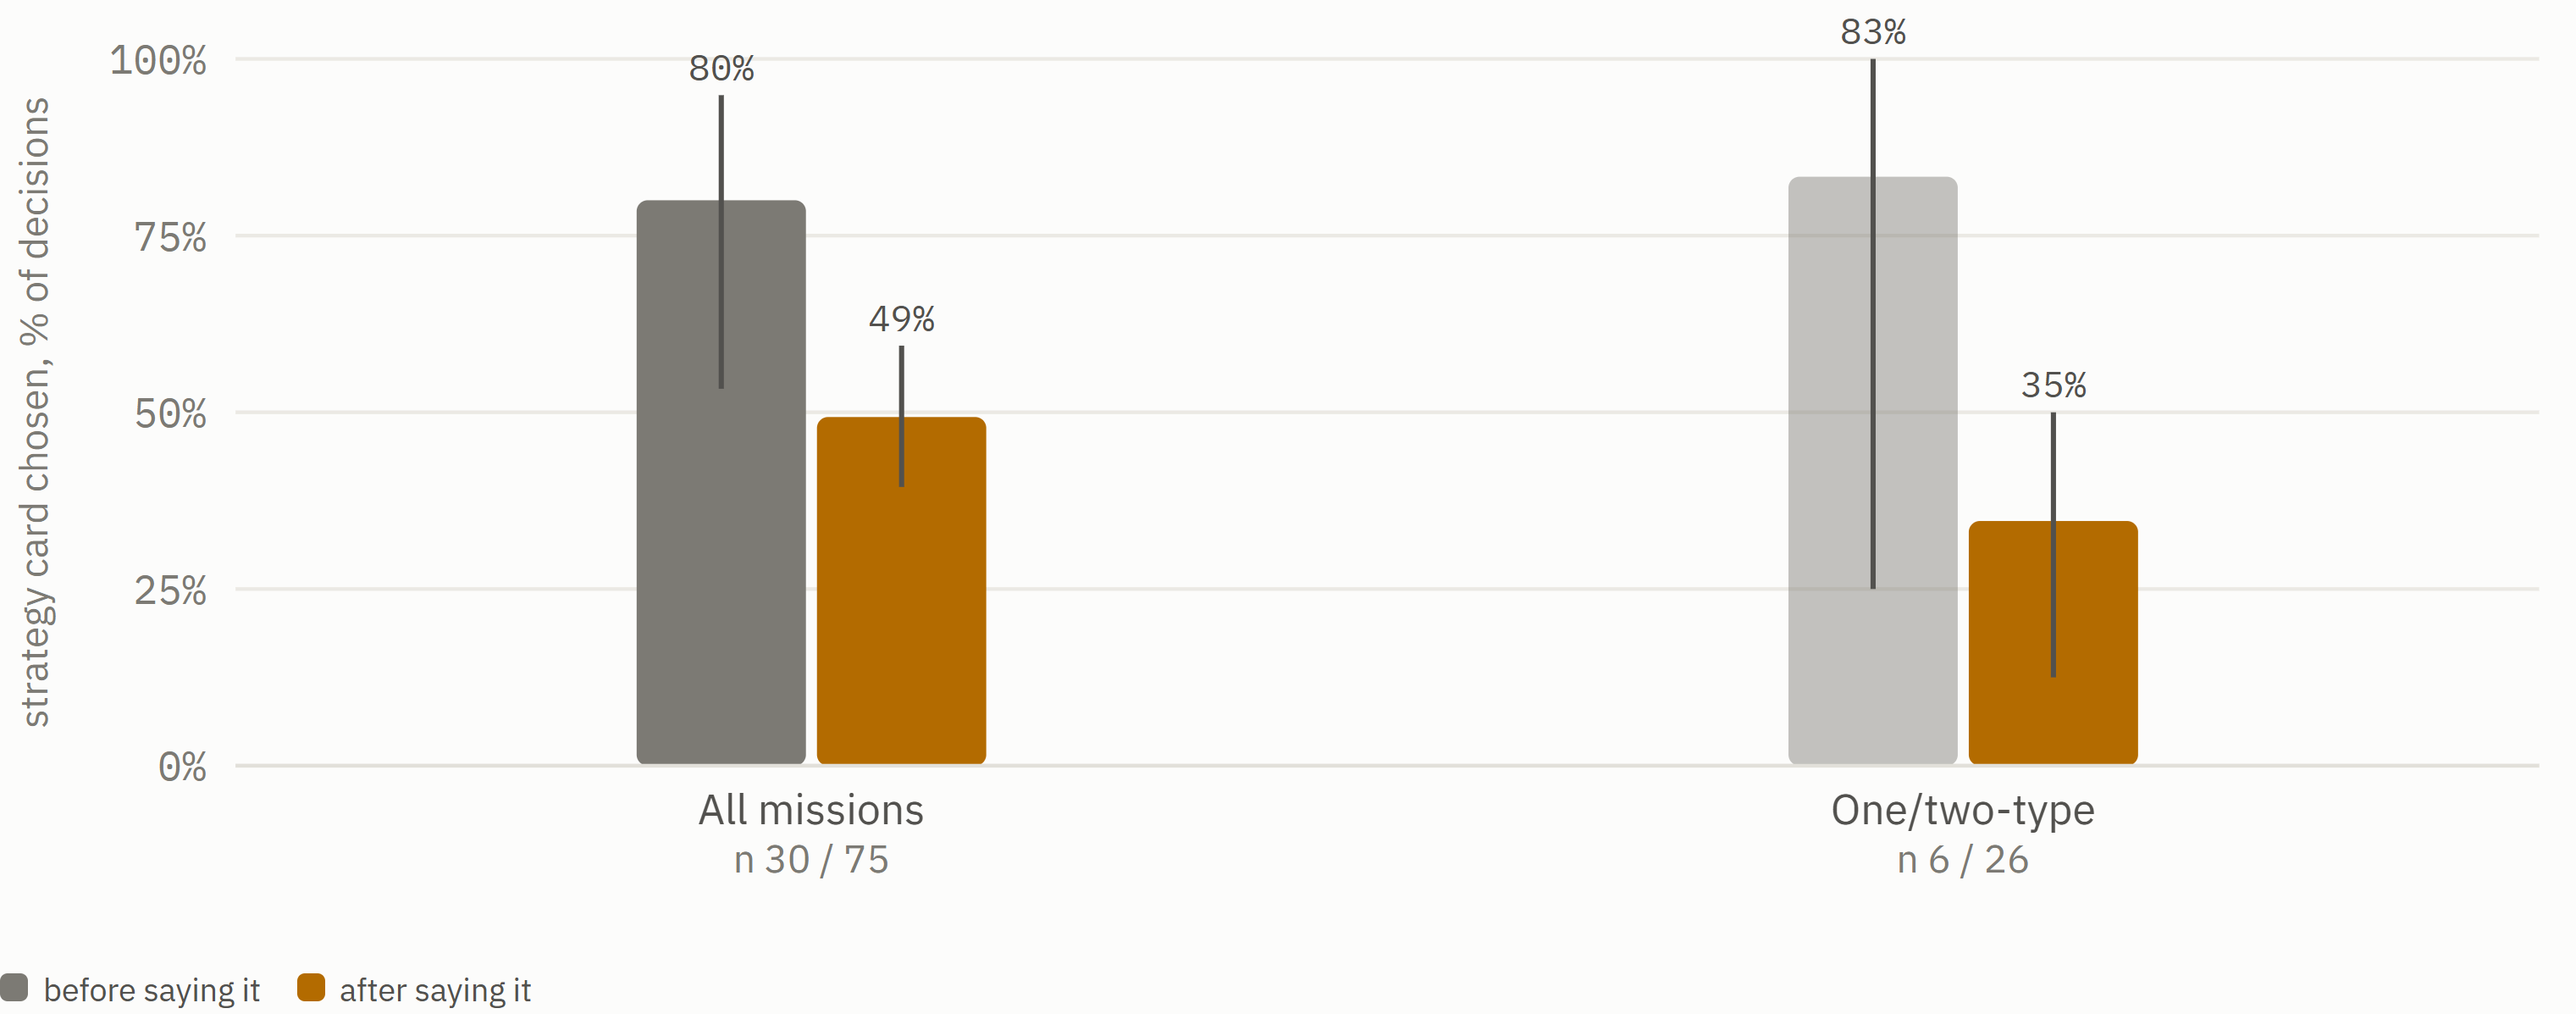
\includegraphics[width=\linewidth,height=0.50\textheight,keepaspectratio]{figs/results/f-flaw-odd__spoken__strict.png}
\caption{\textbf{After saying aloud that a strategy card was wrong, card choice falls (seven people; a direction, not a measured size).} Share of strategic decisions with a strategy card chosen, before and after the remark: all missions, and one- and two-type missions.}
\label{fig:res:flaw-odd:spoken}
\label{fig:res:flaw-odd:spoken:strict}
\end{figure}

\begin{options}
\optshead{Options for this finding}

\optsec{The event study, aligned on the first illogical card (every step, pairs or threes)} {\footnotesize [pass 5: for the paper]}

\par\noindent \begin{minipage}[t]{0.49\linewidth}\centering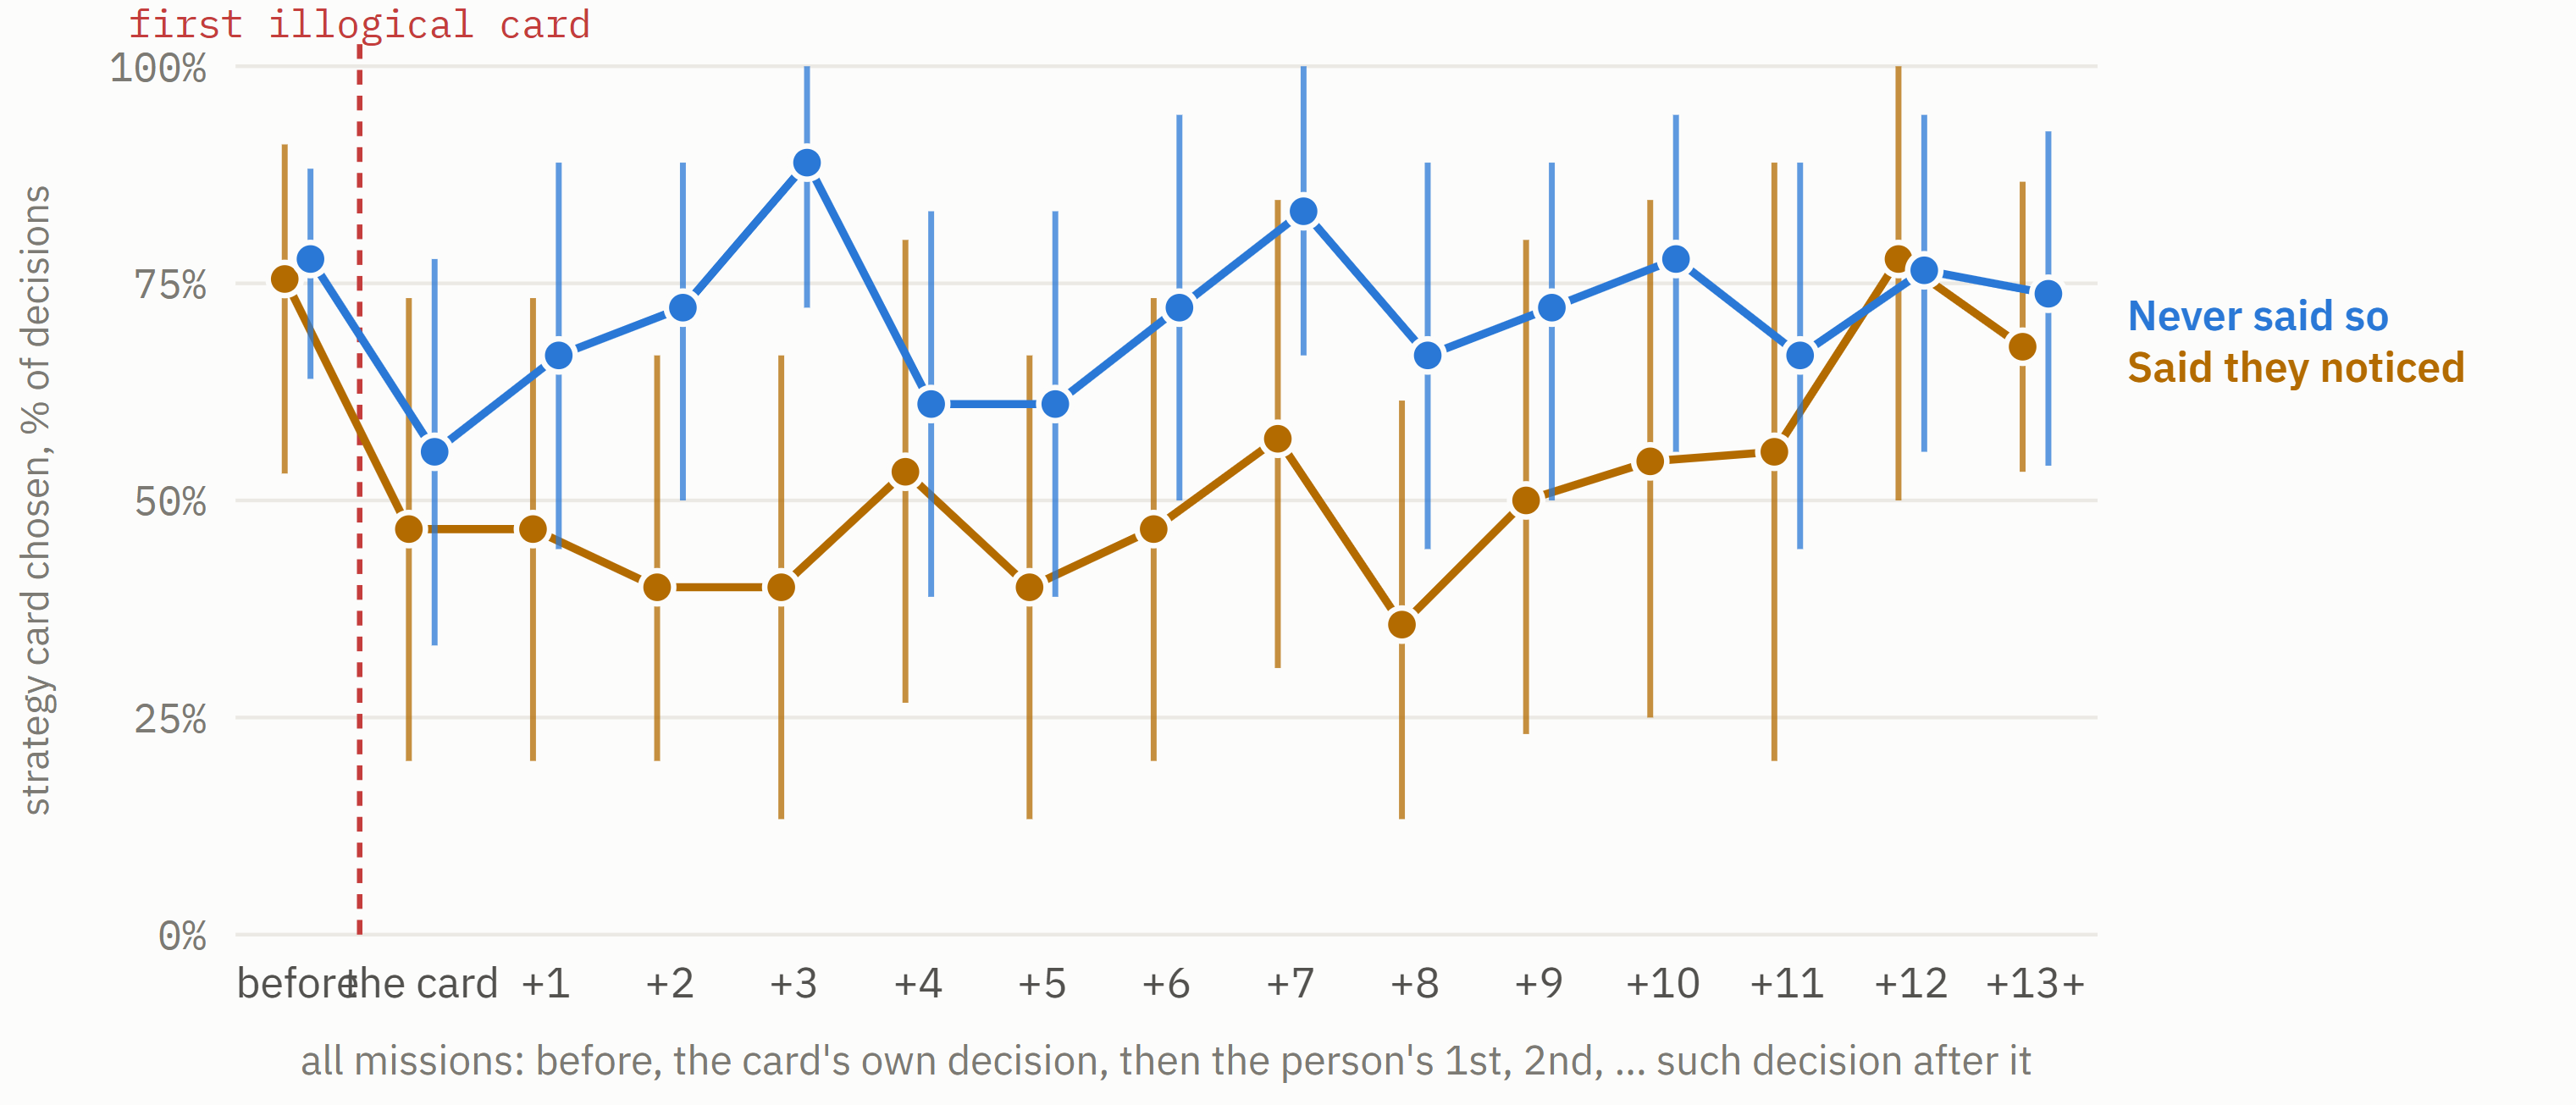
\includegraphics[width=\linewidth,height=0.24\textheight,keepaspectratio]{figs/results/f-flaw-odd__event__steps.png}\par{\scriptsize Other view: All missions, every step.}\end{minipage}

\noindent Key numbers:\begin{itemize}[leftmargin=1.2em,itemsep=0pt]\footnotesize
\item All missions, noticers (15): 76\% before (n 53) $\rightarrow$ card 47\% (n 15) $\rightarrow$ pairs +1--2 to +9--10: 43\%, 47\%, 43\%, 46\%, 52\% $\rightarrow$ 67\% (+11--12) $\rightarrow$ 68\% (13th+, n 31)
\item All missions, never said (18): 78\% before (n 54) $\rightarrow$ 56\% at the card $\rightarrow$ 67--75\% for every later pair
\item All missions, before $\rightarrow$ after, adjusted: noticers $-$14 points, p = .08; never said +9, p = .14; difference $-$14 [$-$30, +1], p = .06
\item Three-type, noticers by pair: 74\% before (n 51), 43\% (n 30), 59\% (n 29), 62\% (n 24), 63\% (n 19), 75\% (n 12)
\item Why expected is lower for noticers: their own-rate term (take rate on all their other decisions) is 56\% vs 70\%; 79\% of a noticer's decisions come at or after the card, where they took 50\% per person vs 72\% (p = .007); before the card the groups were alike (68\% vs 63\%, p = .71)
\item Mission-only expected (own-rate term set to the average): after the card 68\% noticers vs 69\% never-said; before 80\% vs 81\%
\item Steps before the card, all missions: noticers $\leq$$-$4 87\% (n 23), $-$3 88\% (n 8), $-$2 50\% (n 8), $-$1 64\% (n 14); never-said 82\%, 100\%, 88\%, 56\% (n 22, 8, 8, 16)
\item $-$1 against $-$3/$-$2, the 16 people with three steps (all tactical-heavy-first): adjusted $-$13 points [$-$40, +13], p = .29
\item Matched view (8 noticers with 3+ steps, 6 of whom met the card at the start of session 2): 87\%, 88\%, 50\%, 63\% before $\rightarrow$ 38\% at the card $\rightarrow$ 31--44\% for the next ten decisions
\end{itemize}

\noindent Highlighted quotes not used above:\begin{quotelist}
\item ``Why is it that the green ones, there's no green or red, unless I'm missing something.''\,---\,P17 (think-aloud s1 5:25)
\item ``And then when it came to assigning them, I noticed, oh, okay, it's made a mistake.''\,---\,P20 (debrief 0:26:11)
\item ``where we can go conservative, but we don't need any, in this one we don't need any lifter or cameras.''\,---\,P30 (think-aloud s1 1:01)
\item ``But I find that the first task it allocated too much Lifter and Camera. So I think I'm less confident for it.''\,---\,P35 (think-aloud s1 1:22)
\item ``there was one example in the first round where it was required all fast drones. And I think the AI assistant recommended I add some red and green drones.''\,---\,P20 (debrief 0:25:51)
\item ``I mean, it was giving me the wrong type of drones. It required only blue drones and kept giving me red and green ones.''\,---\,P21 (debrief 0:35:03)
\item ``deploy a conservative strategy for that one doesn't make sense, I don't think. Because I don't need any red or blue drones.''\,---\,P20 (think-aloud s1 3:41)
\end{quotelist}

\optsec{Card use through the session, noticers and never-said} {\footnotesize [pass 5: for the paper]}

\noindent Key numbers:\begin{itemize}[leftmargin=1.2em,itemsep=0pt]\footnotesize
\item Session 1, noticers by minute 0--1 to 4--5: 86\% (n 21), 50\% (n 16), 50\% (n 14), 38\% (n 16), 73\% (n 11)
\item Session 1, never said: 65\% (n 31), 71\%, 88\%, 76\%, 69\%
\item Session 2, noticers: 52\% (n 29), 53\%, 53\%, 38\% (n 13), 38\% (n 21), 55\%, 73\%, 60\%; never said 61--89\%
\end{itemize}

\noindent Highlighted quotes not used above:\begin{quotelist}
\item ``I know there is a better choice, but I have no time to tune everything.''\,---\,P28 (debrief 0:30:33)
\end{quotelist}

\optsec{Card use by decision number, session 1 then session 2, not aligned to the card} {\footnotesize [pass 5: for the paper]}

\par\noindent \begin{minipage}[t]{0.49\linewidth}\centering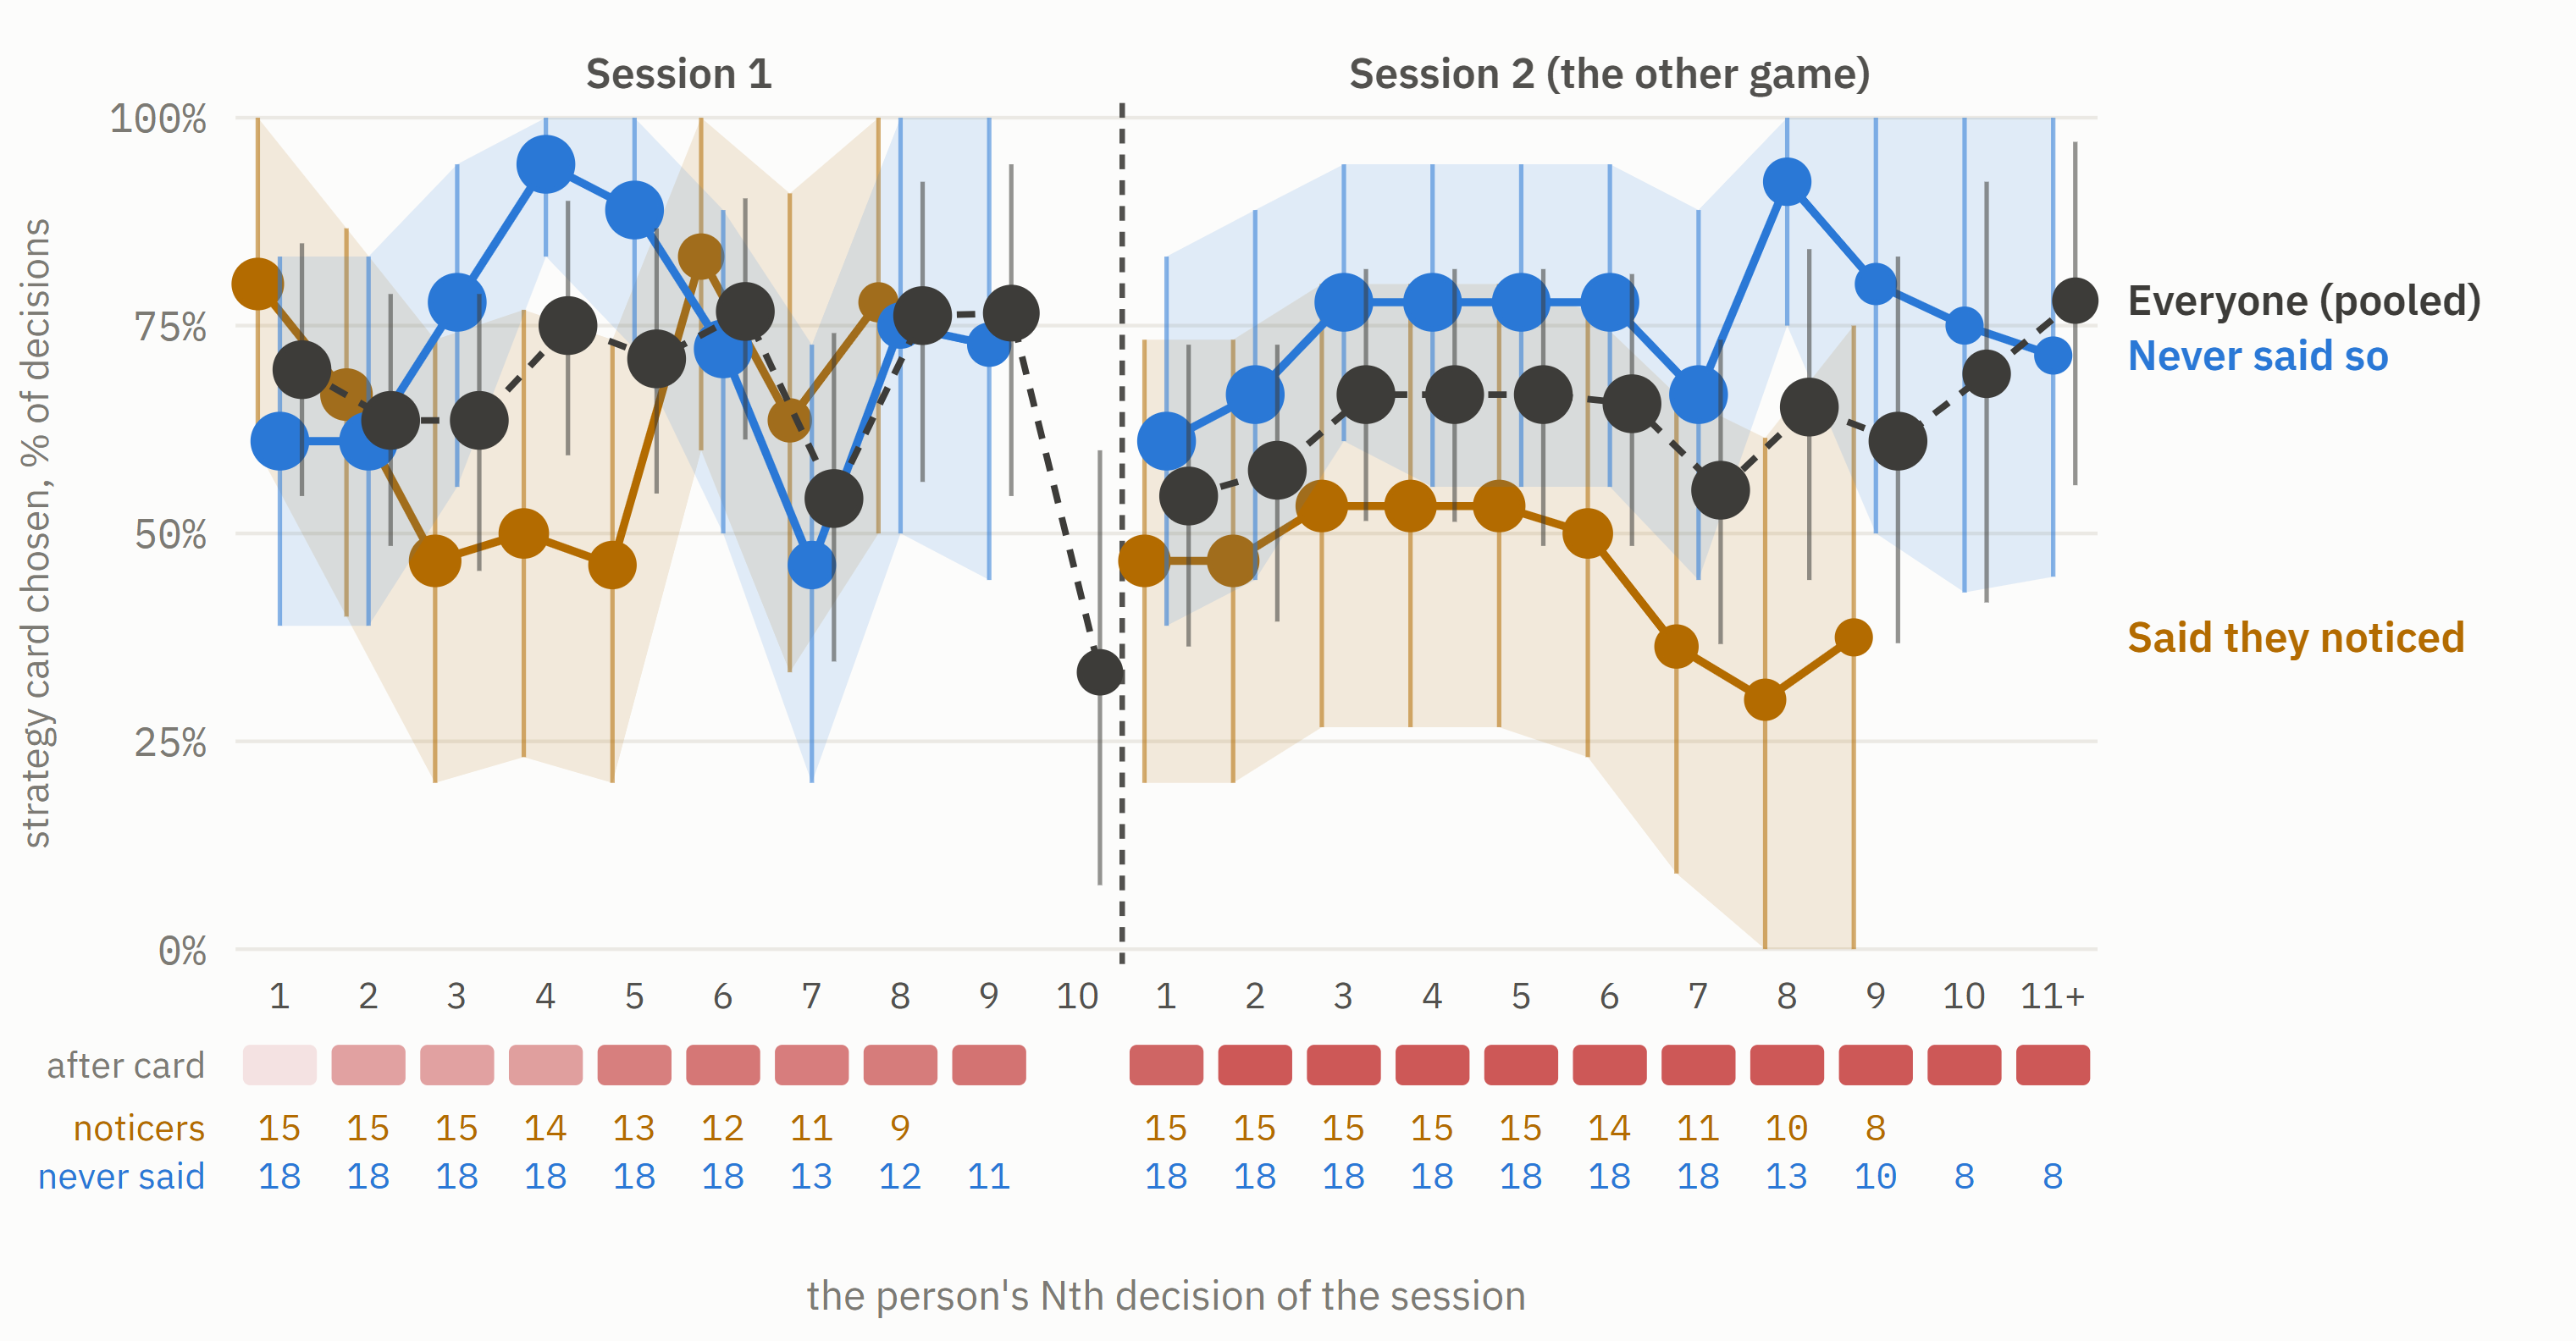
\includegraphics[width=\linewidth,height=0.24\textheight,keepaspectratio]{figs/results/f-flaw-odd__by-index__everyone.png}\par{\scriptsize Other view: Each group and everyone.}\end{minipage}

\noindent Key numbers:\begin{itemize}[leftmargin=1.2em,itemsep=0pt]\footnotesize
\item Everyone, session 1, decisions 1--6: 70\%, 64\%, 64\%, 75\%, 71\%, 77\% (n 33 $\rightarrow$ 30)
\item Noticers, session 1: 80\%, 67\%, 47\%, 50\%, 46\%, 83\%, 64\%, 78\% (decisions 1--8, 15 $\rightarrow$ 9 people); never said: 61\%, 61\%, 78\%, 94\%, 89\%, 72\%, 46\%, 75\%, 73\% (decisions 1--9, 18 $\rightarrow$ 11 people)
\item Session 1 fixed panel (9 noticers, 12 never-said, decisions 1--8): noticers 78, 67, 56, 44, 44, 89, 56, 78\%; never said 50, 42, 67, 92, 83, 67, 50, 75\%
\item Session 1 tail (hidden): decision 9, 6 noticers 83\%; decision 10, 5 noticers 1 of 5 took (20\% [4, 62]), 7 never-said 43\% [16, 75]; 11+, 2 noticers 3 of 7 (one took 3 of 4, the other 0 of 3), 5 never-said 7 of 12. All strategic-heavy-game players; 57--67\% of the 11+ decisions in the last 90 s
\item Session 2 tail (hidden for noticers): decision 10, 5 noticers 60\%; 11+, 4 noticers (all tactical-heavy first, so playing the strategic-heavy game) 12 of 13 = 92\% [67, 99], against 8 never-said 20 of 28 = 71\%. These 4 took cards on 42\% of their decisions 1--6, below their group's 51\%: not keen takers surviving
\item Strategic-heavy game: share of decisions with an illogical card at decisions 7, 8, 9, 10, 11+: 48\%, 55\%, 30\%, 4\%, 5\%. At decisions 7+, noticers took 17\% of illogical-card missions (n 18, 9 people) and 62\% of the rest (n 53); never-said 68\% and 69\%
\item Session 2, no illogical card: noticers 71\% at decisions 7 and 8 (7 people) against never-said 73\% and 70\%; earlier the gap is there (decisions 2--3: 33--47\% against 67--89\%)
\item Session 2 fixed panel (8 noticers, 10 never-said, decisions 1--9): gap over the last 3 decisions $-$47 points [$-$81, $-$12] against $-$19 [$-$50, +12] before; on missions with no illogical card (panel to decision 6) $-$17 [$-$45, +12] against $-$30 [$-$61, +1]
\item At the session break (last 3 of session 1 $\rightarrow$ first 3 of session 2): noticers 64\% $\rightarrow$ 49\%, $-$16 points [$-$38, +4], p = .17; adjusted $-$9 [$-$30, +12]; never-said 76\% $\rightarrow$ 69\%, $-$7 [$-$24, +7]; difference $-$6 [$-$32, +20], p = .66
\item Recovery within session 1 (decisions 3--5 $\rightarrow$ 6+): noticers 48\% (n 42) $\rightarrow$ 66\% (n 50), +24 points per person [+5, +43], p = .04 (window read off the curve, so descriptive)
\end{itemize}

\optsec{Lined up on the moment they said a strategy card was wrong: card use falls (7 people, a direction only)} {\footnotesize [pass 5: for the paper]}

\par\noindent \begin{minipage}[t]{0.49\linewidth}\centering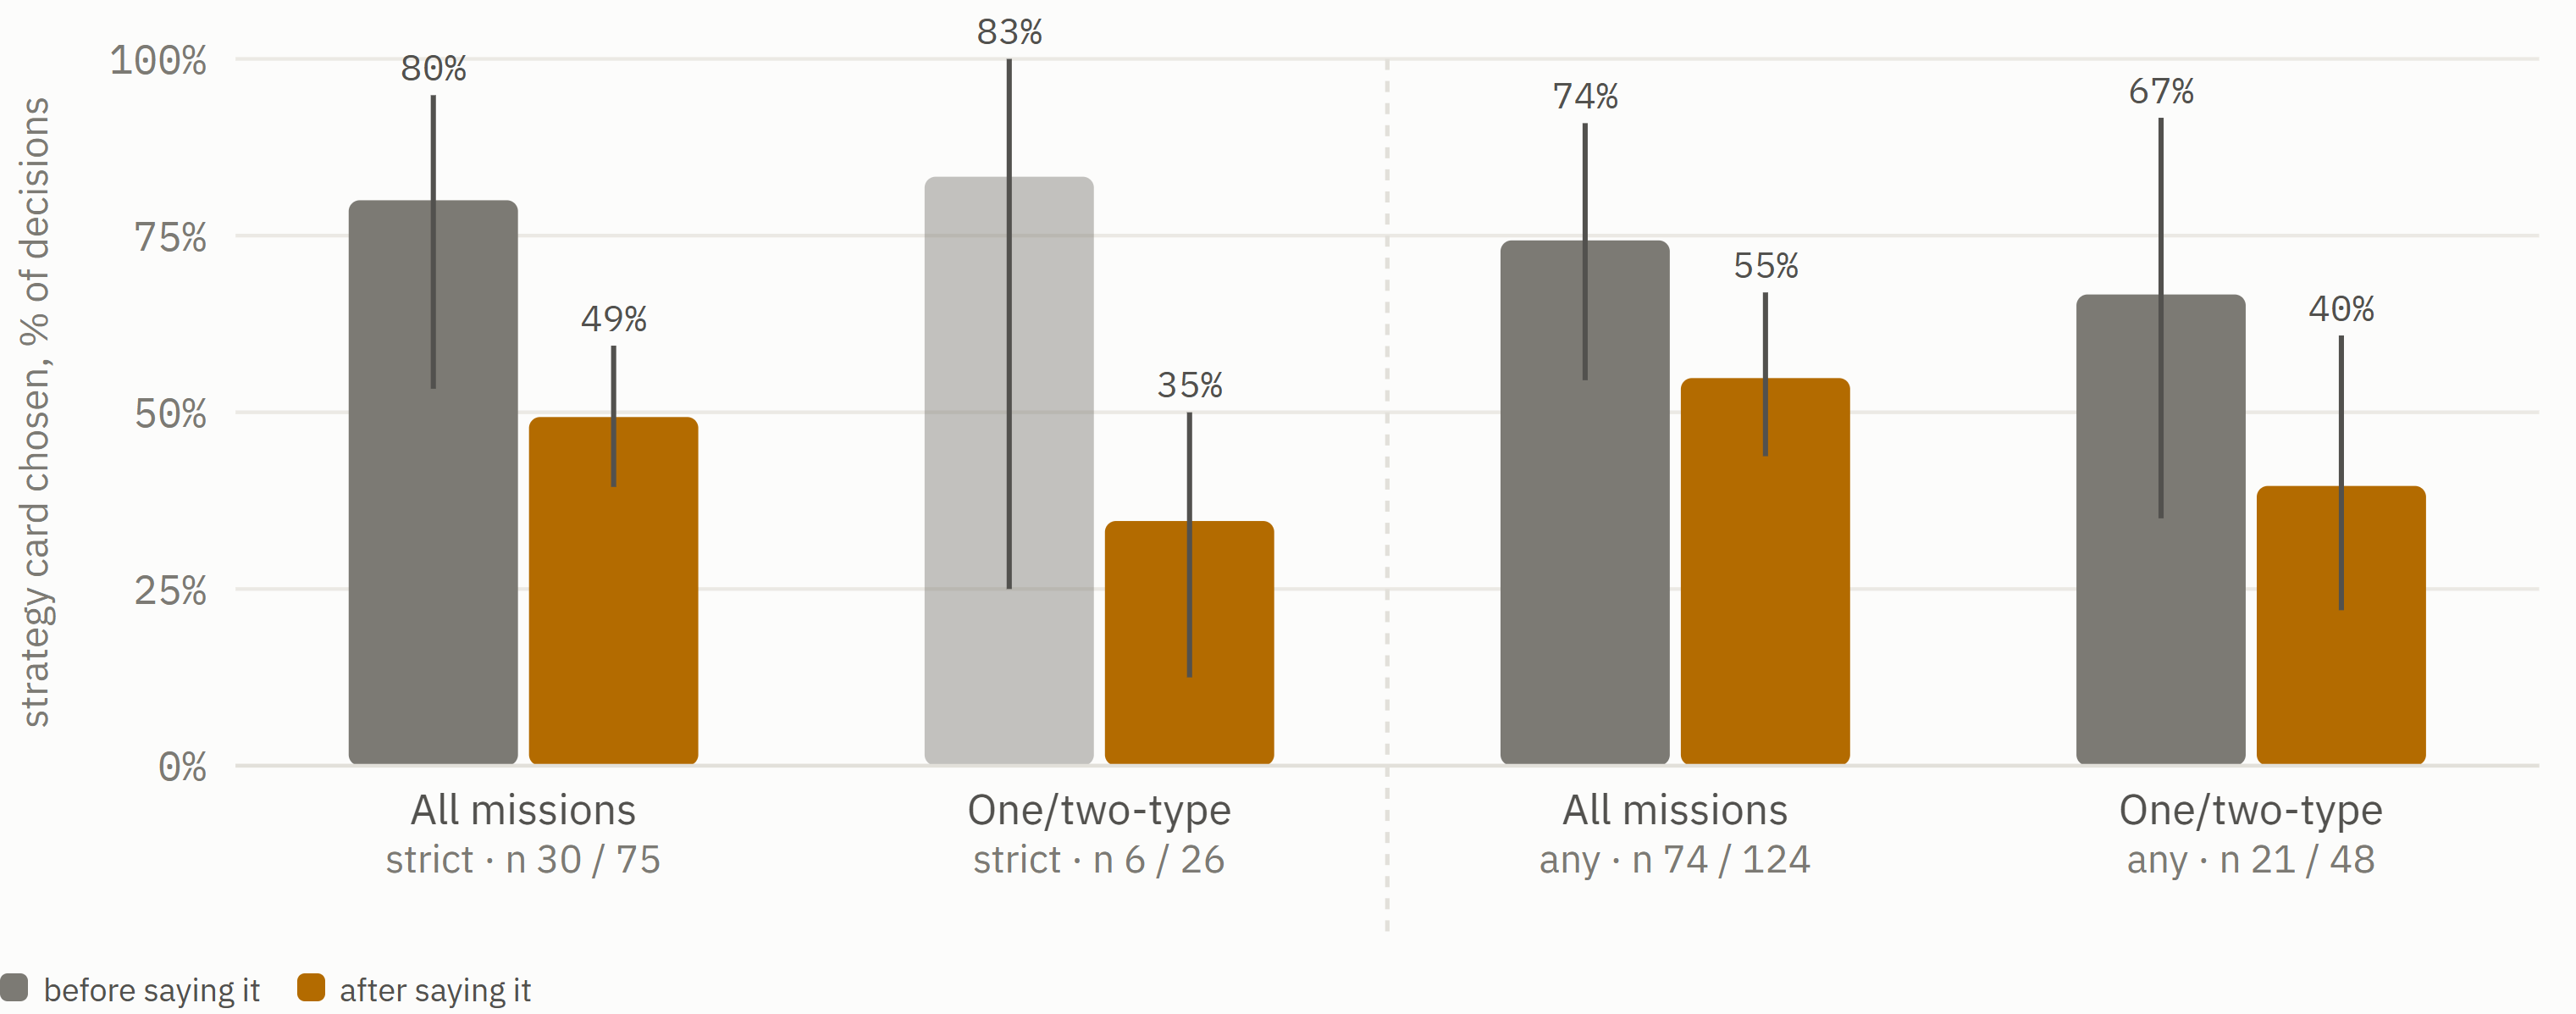
\includegraphics[width=\linewidth,height=0.24\textheight,keepaspectratio]{figs/results/f-flaw-odd__spoken__any.png}\par{\scriptsize Other view: Strict and any remark, side by side.}\end{minipage}

\noindent Key numbers:\begin{itemize}[leftmargin=1.2em,itemsep=0pt]\footnotesize
\item Strict remarks (7 people), all missions: 80\% (n 30) $\rightarrow$ 49\% (n 75); adjusted $-$21 points [$-$49, +7], p = .11; 5 fell, 2 rose; placebo p = .51
\item Strict, one/two-type: 83\% (n 6, 4 people) $\rightarrow$ 35\% (n 26, 7 people); three-type: 79\% (n 24) $\rightarrow$ 57\% (n 49)
\item Any remark (12 people), all missions: 74\% (n 74) $\rightarrow$ 55\% (n 124), adjusted $-$4 points, p = .60; one/two-type 67\% (n 21) $\rightarrow$ 40\% (n 48)
\end{itemize}

\optsec{A different event: after the Tactical Assistant's first 'No workable plan', nothing changes on either tier} {\footnotesize [pass 5: numbers only]}

\par\noindent \begin{minipage}[t]{0.49\linewidth}\centering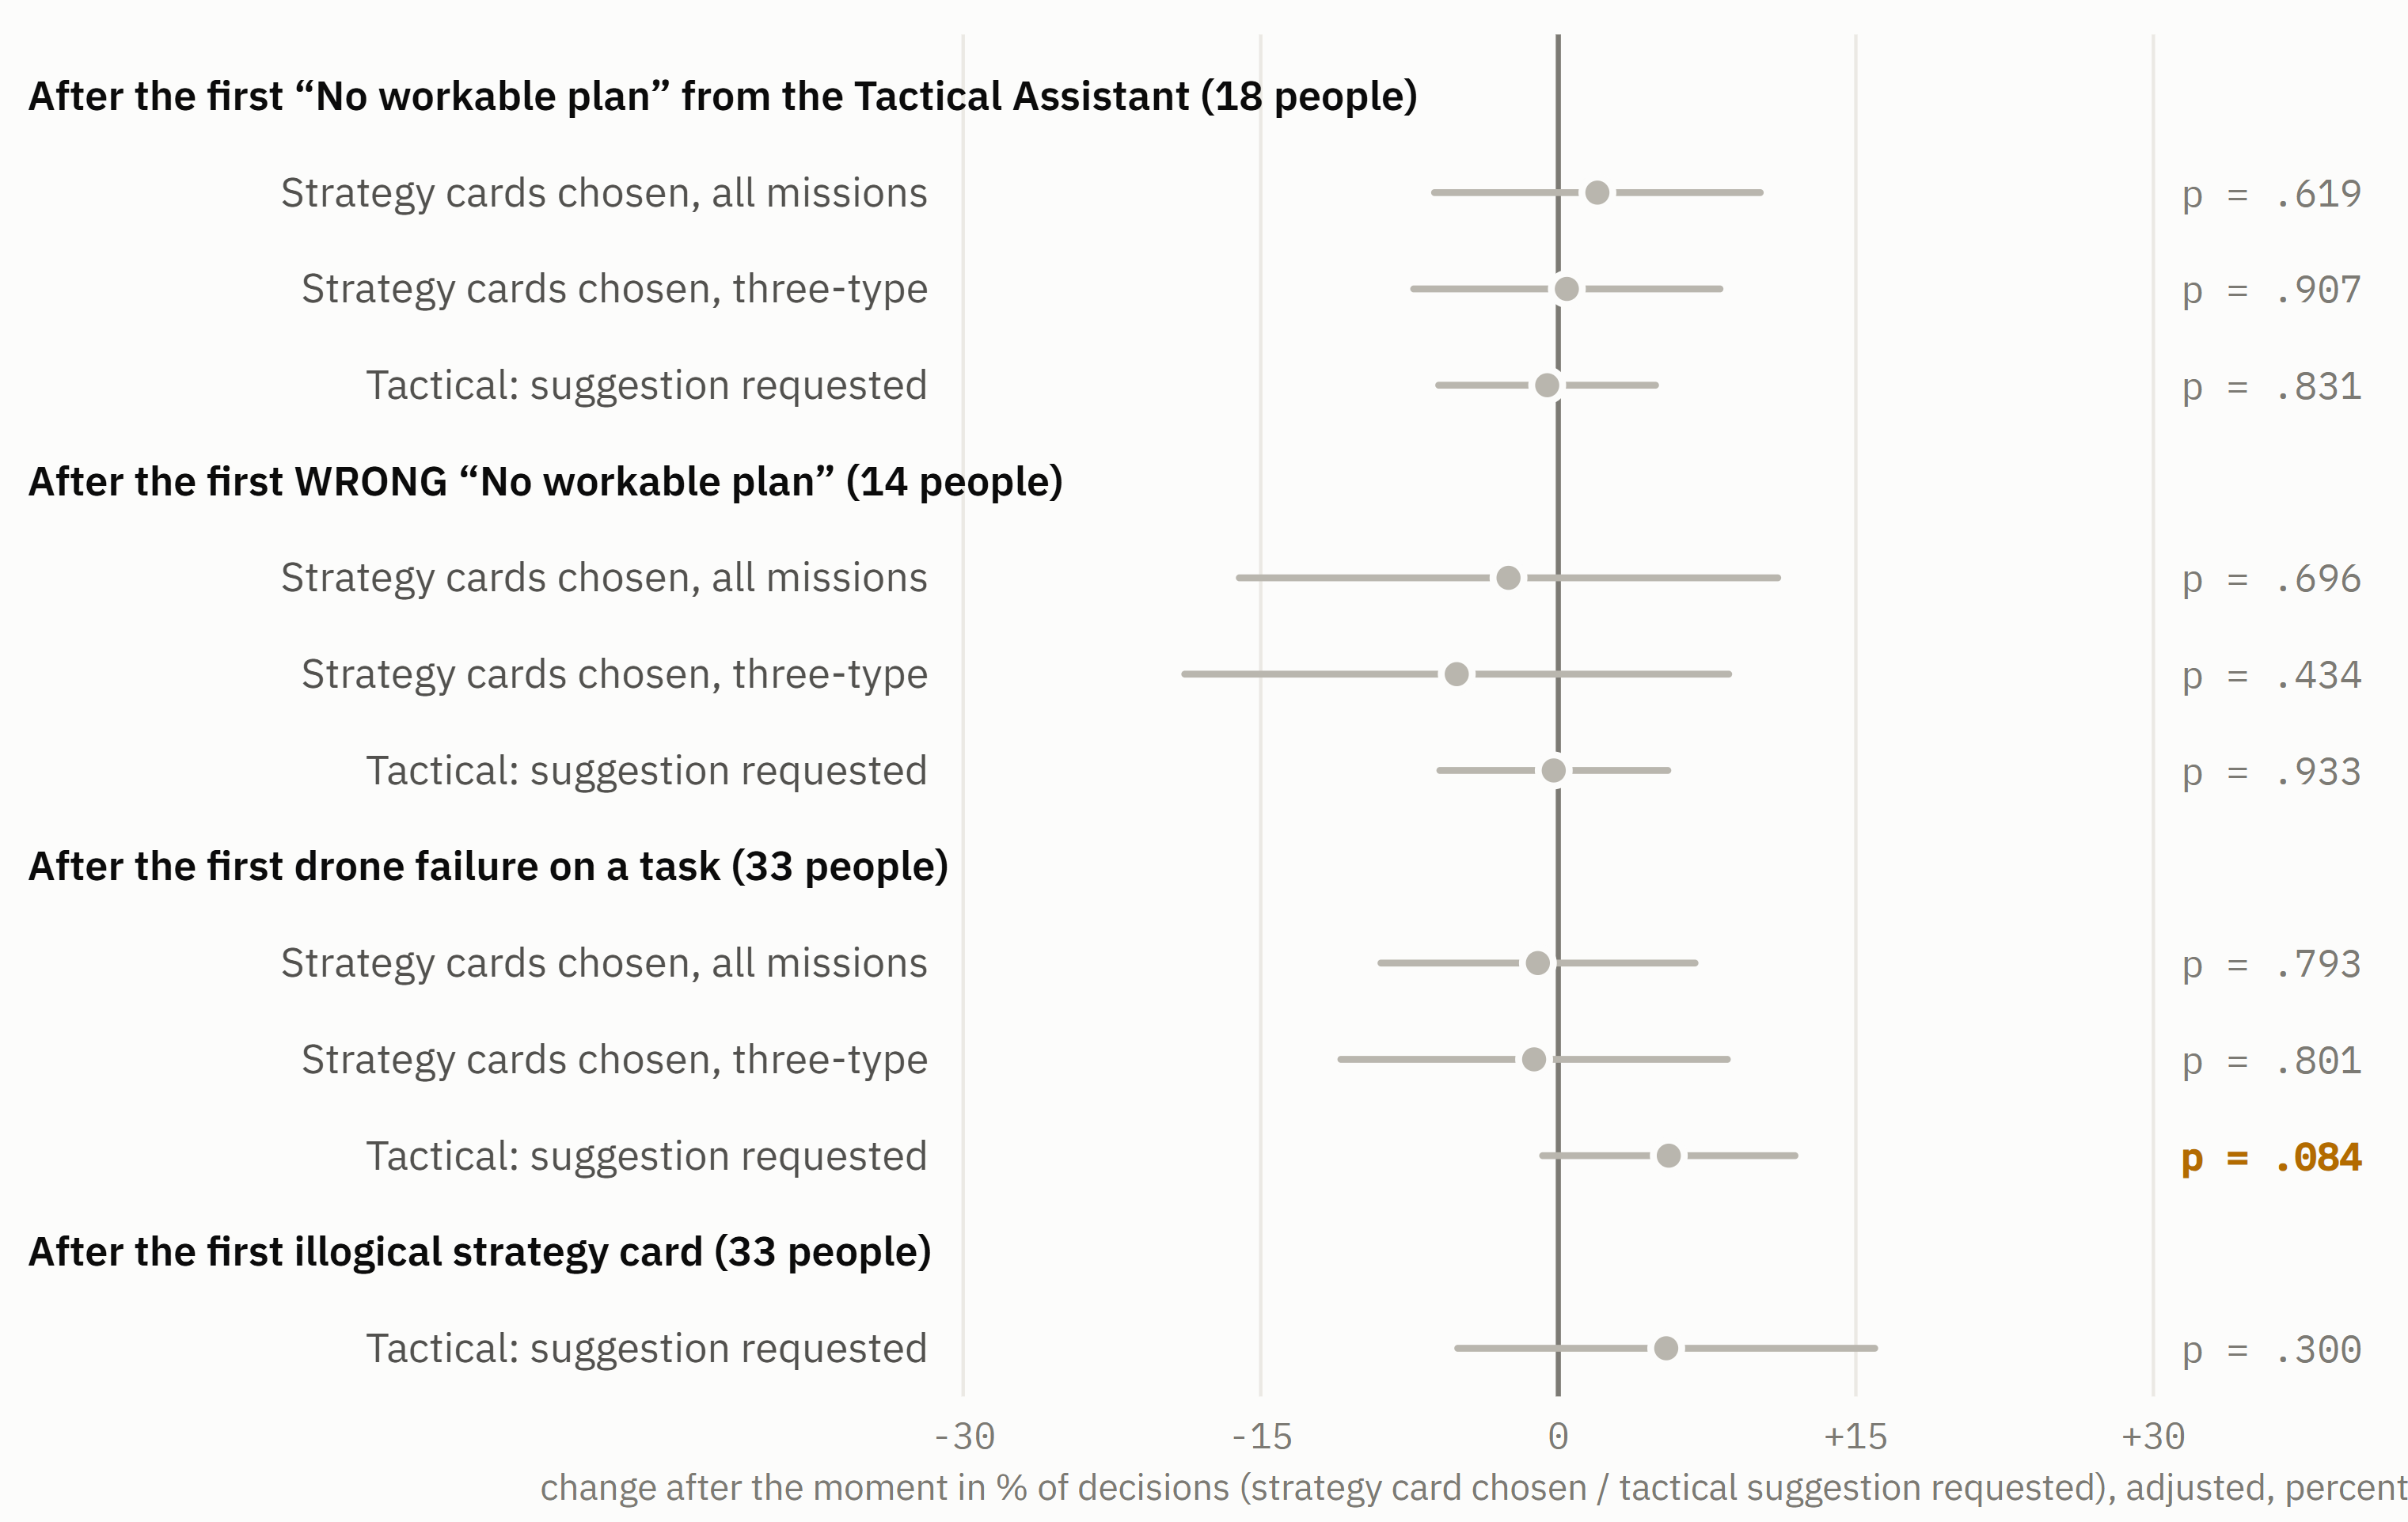
\includegraphics[width=\linewidth,height=0.24\textheight,keepaspectratio]{figs/results/f-flaw-odd__refusal__main.png}\par{\scriptsize Other view: main}\end{minipage}

\noindent Key numbers:\begin{itemize}[leftmargin=1.2em,itemsep=0pt]\footnotesize
\item First refusal (18): strategy cards, all missions, adjusted +2.0 points [$-$6, +10], p = .62; three-type +0.4, p = .91; tactical Suggest $-$0.6 [$-$6, +5], p = .83
\item First WRONG refusal (14): strategy cards $-$2.5 [$-$16, +11], p = .70; three-type $-$5.1, p = .43; tactical $-$0.2, p = .93
\item First drone failure (33): strategy cards $-$1.0, p = .79; tactical +5.6, p = .08
\item After the first illogical card, tactical Suggest +5.4 points, p = .30 (no spill-down either)
\end{itemize}

\optsec{Why the pre-registered test (H8) was dropped} {\footnotesize [not used in the prose above]}

\noindent\regtext{H8 asked whether uptake falls after an operator 'realises' the card can be illogical. Its marker for that realisation was the first time a person went manual on an illogical-card mission and left out the unneeded type. The trouble is that, by that definition, every illogical-card decision \emph{before} the marker was not such a manual choice. So the 'before' window was mostly forced to be card takes, near 100\%. Any later manual choice then shows up as a drop, even if the person never changed at all. A simulation confirmed it. In simulated people who keep the same habits all study, the same marker produced a large 'drop' (average odds ratio 0.37, against the real 0.12). Measured against that, the real drop was ordinary (calibrated p = .30, about $-$10 points after correction). Defining the marker as the first manual choice on a \emph{clean} card produced the same kind of drop. H8 was replaced by tests whose anchor is not defined by the outcome (the first illogical card shown; the moment someone said it), each checked against a placebo. Those are the tests in this finding.}

\noindent Key numbers:\begin{itemize}[leftmargin=1.2em,itemsep=0pt]\footnotesize
\item Pre-registered estimate OR 0.12; the same test on no-change simulations averages OR 0.37; calibrated p = .30 (risk difference)
\item Placebo marker on clean cards: OR 0.22, p = .03, the same kind of 'drop'
\end{itemize}
\end{options}

\clearpage

% ======== f-tier-trust ========

\subsection{The Tactical Assistant is trusted more}\label{sec:res:tier-trust}

On the questionnaire after each session, operators trusted the Tactical Assistant more than the Strategic Assistant (5.44 against 4.61 on a 1--7 scale; 26 of 33 people higher for the tactical, $p = .001$). Most of the gap opened in the second session and in the Strategic Heavy games. Tactical plans got only a few seconds of checking, whatever their size.

% --- f-tier-trust#gap (pass 5: for the paper) ---

\phantomsection\label{sec:res:tier-trust:gap}
The gap is a medium-sized effect (mean $+0.83$ points, $d_z = .62$), and every one of the six questionnaire items points the same way (Figure~\ref{fig:res:tier-trust:gap}). The usual reason given is that the strategy cards visibly wasted drones while the tactical plans matched what the operator would have done: ``So the tactical one seemed to be doing what I was doing. So quite reliably. And obviously the strategic one wasn't.'' (P32). Another put it in terms of blame: ``You can't blame the tactical for drone failures but you can blame the strategic for not having redundancy'' (P03).

\begin{figure}[H]
\centering
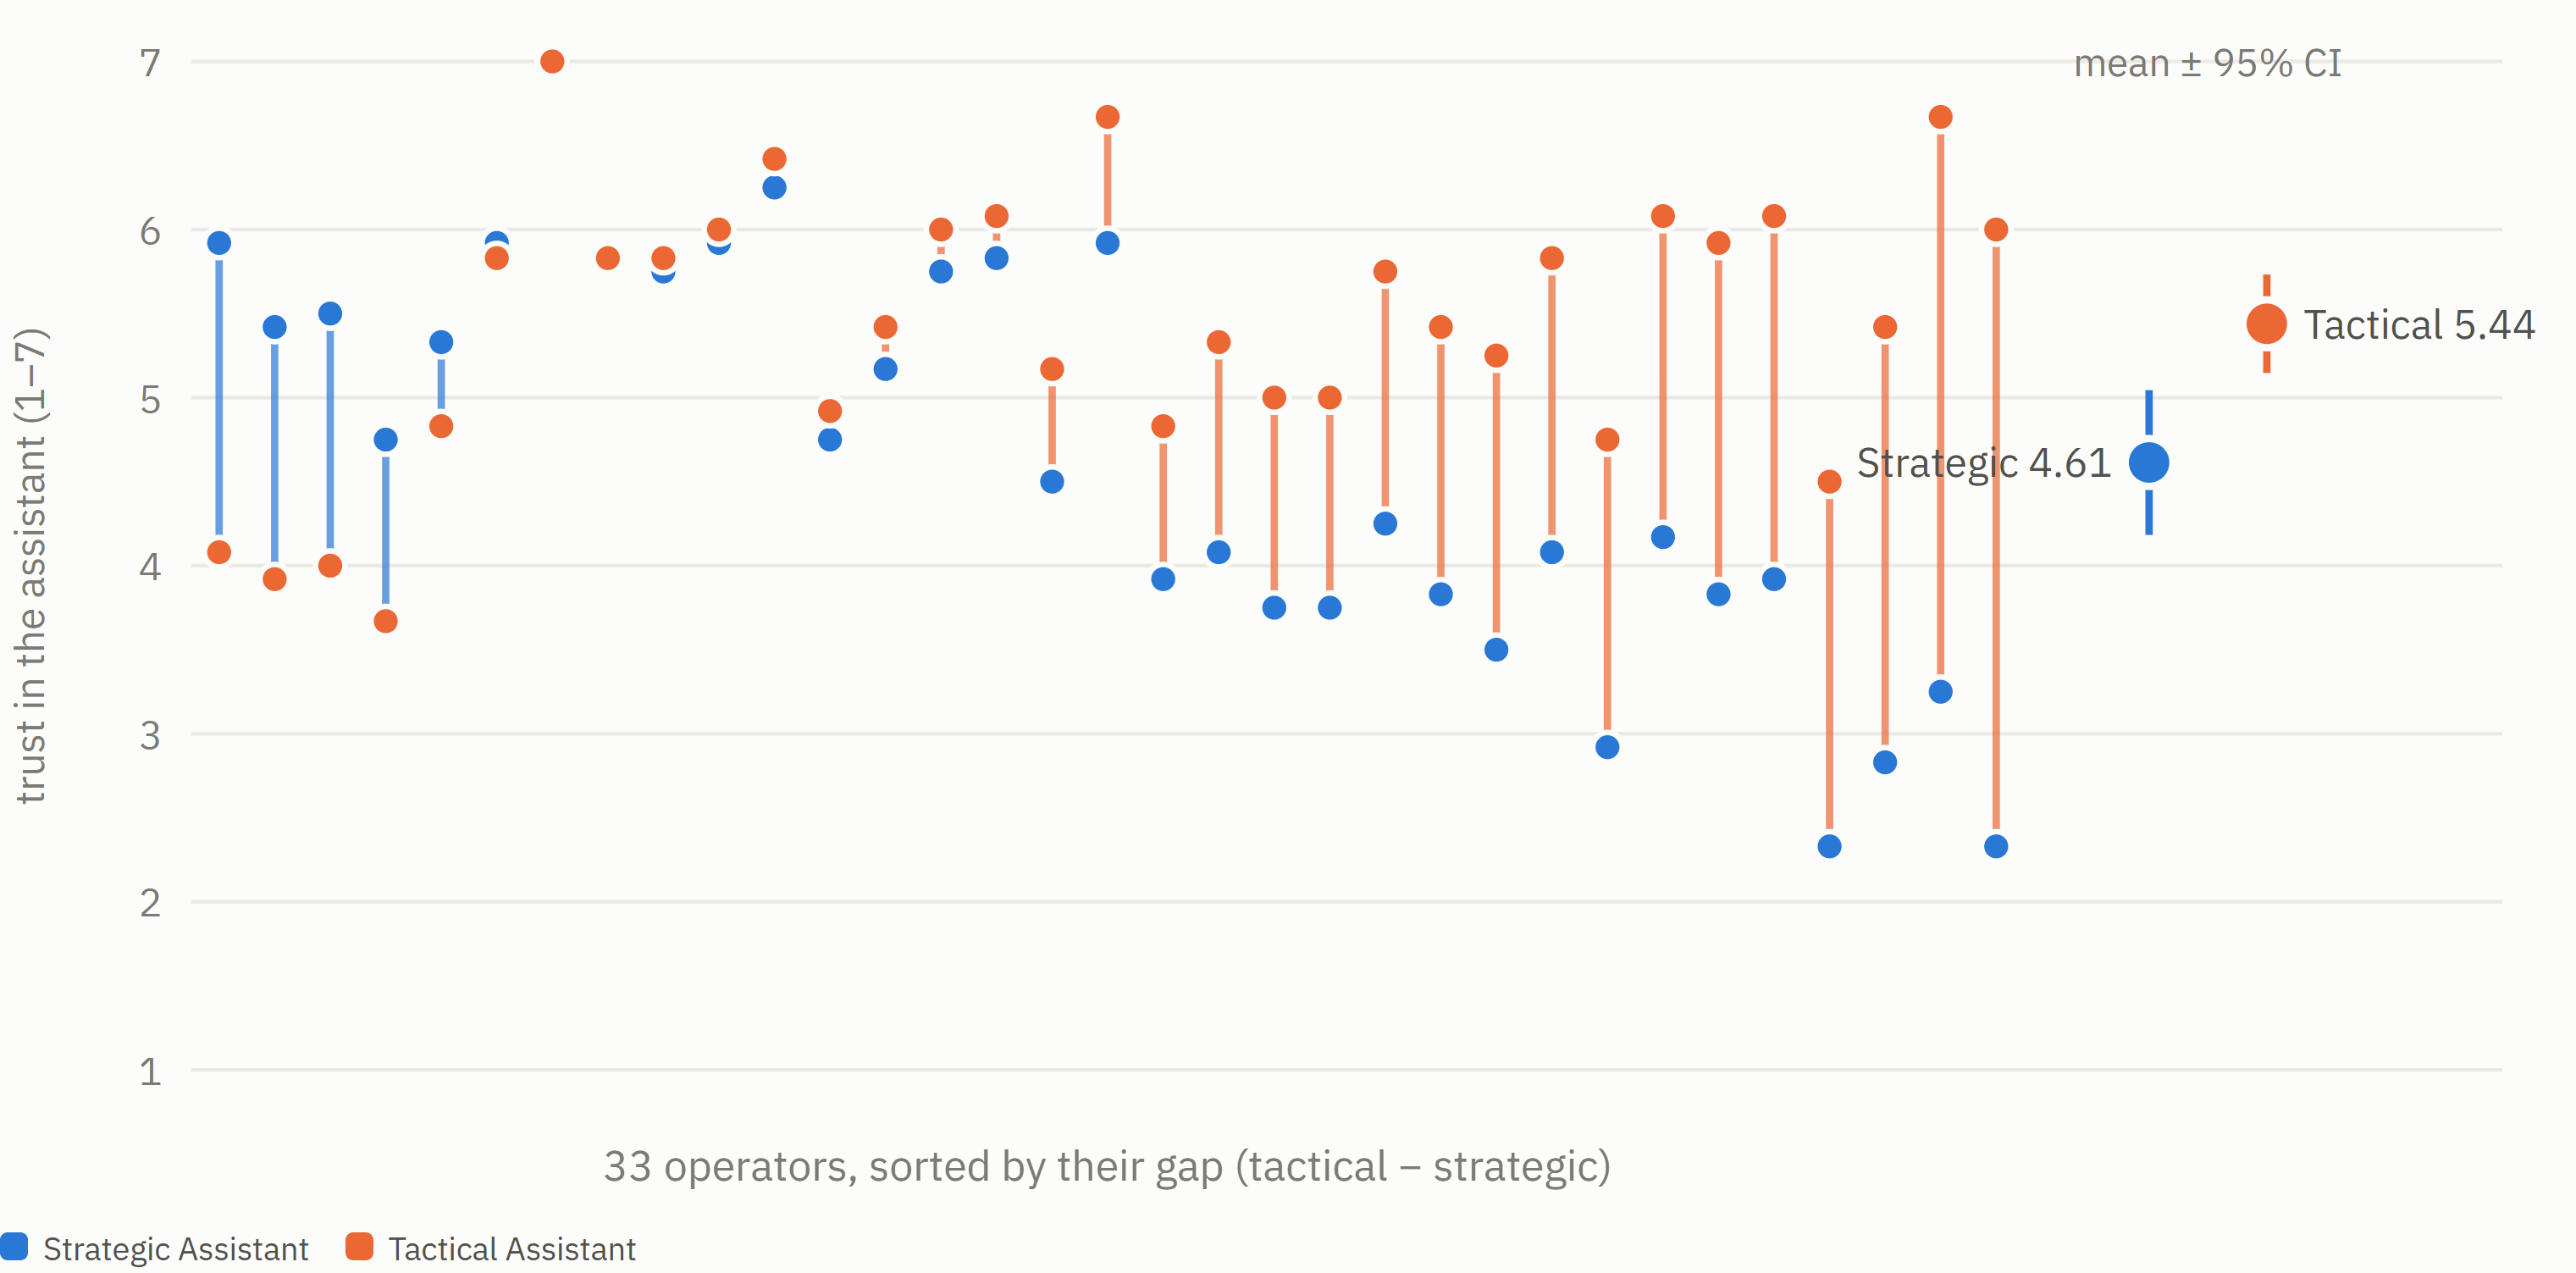
\includegraphics[width=\linewidth,height=0.50\textheight,keepaspectratio]{figs/results/f-tier-trust__gap__main.png}
\caption{\textbf{The Tactical Assistant is trusted more.} Each person's mean trust in each assistant over their two sessions (1--7).}
\label{fig:res:tier-trust:gap}
\end{figure}

% --- f-tier-trust#where (pass 5: for the paper) ---

\phantomsection\label{sec:res:tier-trust:where}
The gap was larger in Strategic Heavy sessions ($+1.13$) than in Tactical Heavy ones ($+0.52$), and small after the first session ($+0.37$) but large after the second ($+1.28$); with both in one model, Strategic Heavy adds about 0.6 to the gap and the second session about 0.9 (Figure~\ref{fig:res:tier-trust:where}). Trust in the Tactical Assistant hardly moved (5.36 to 5.51 across sessions): it is trust in the Strategic Assistant that fell, and most in the scenario where its cards are used most.

\begin{figure}[H]
\centering
\begin{subfigure}[t]{\linewidth}
\centering
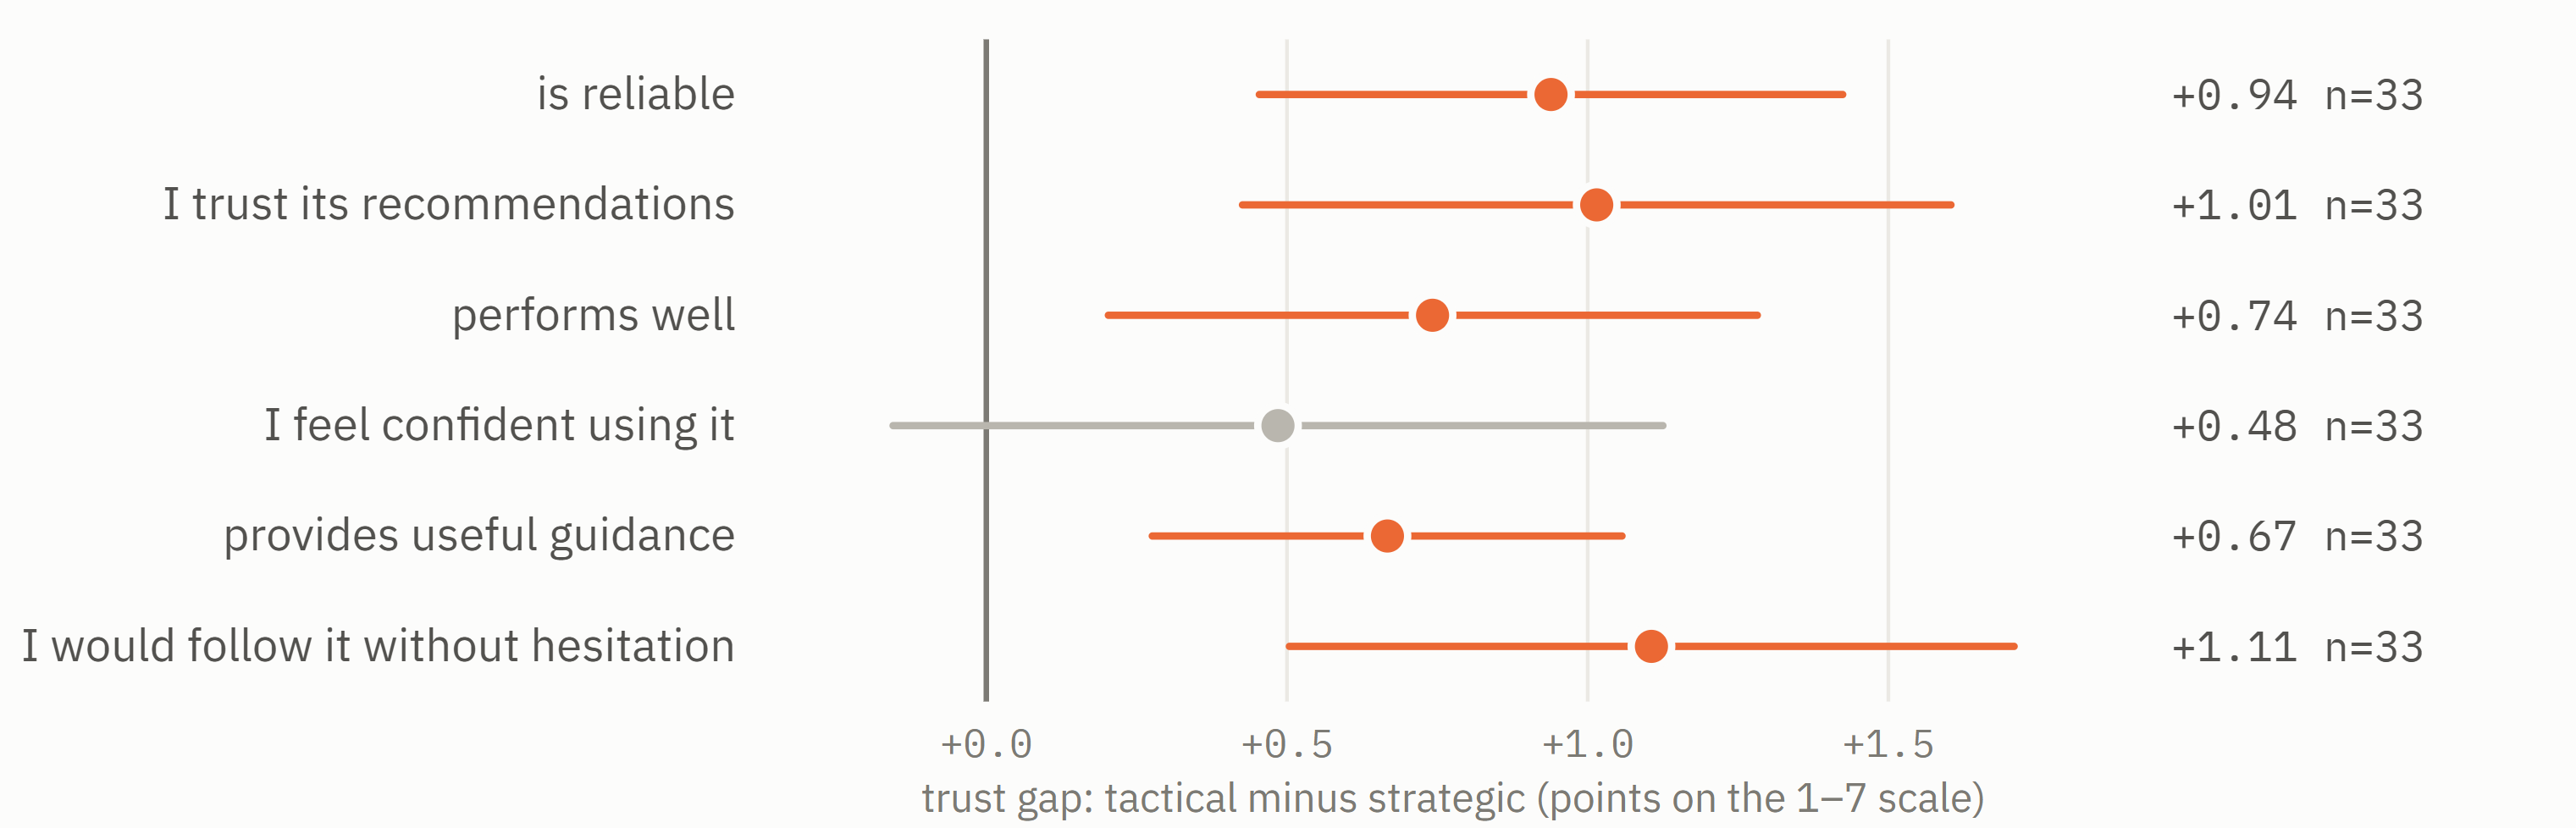
\includegraphics[width=\linewidth,height=0.21\textheight,keepaspectratio]{figs/results/f-tier-trust__where__items.png}
\caption{By questionnaire item.}
\label{fig:res:tier-trust:where:items}
\end{subfigure}
\par\smallskip
\begin{subfigure}[t]{\linewidth}
\centering
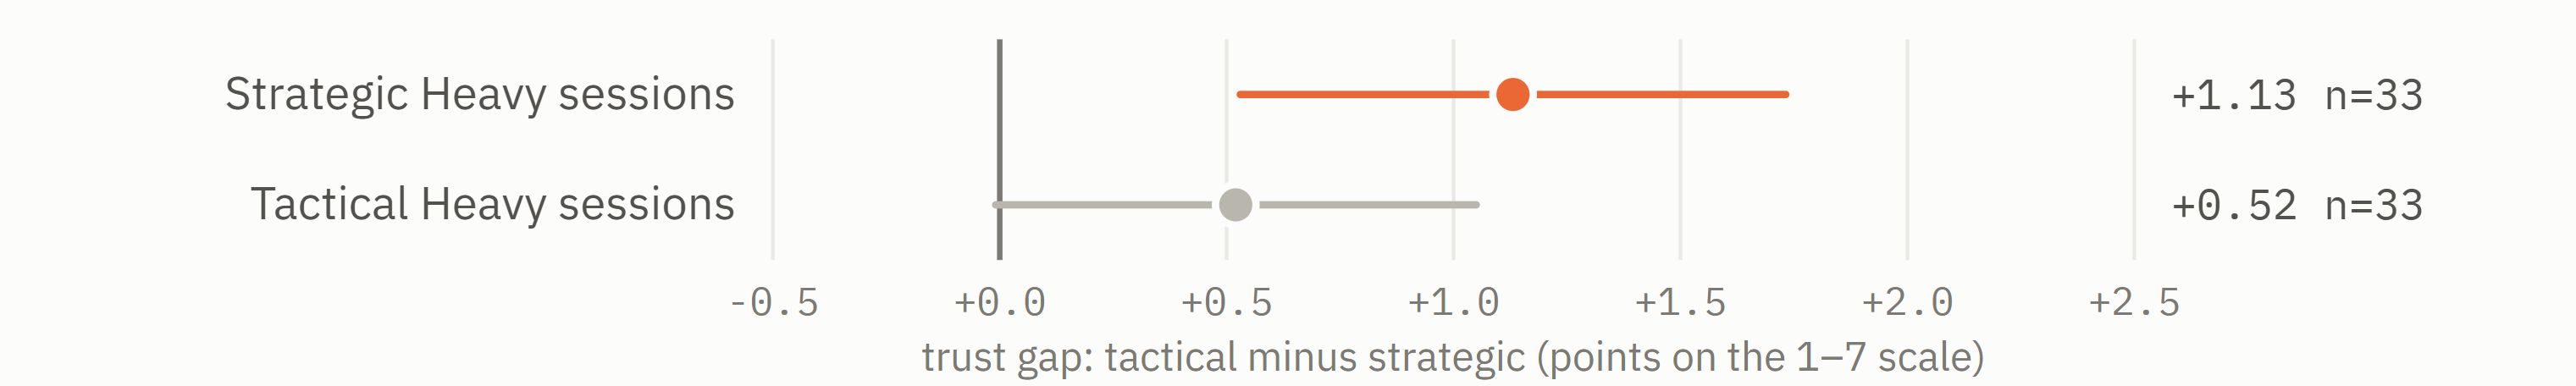
\includegraphics[width=\linewidth,height=0.21\textheight,keepaspectratio]{figs/results/f-tier-trust__where__scenario.png}
\caption{By scenario played.}
\label{fig:res:tier-trust:where:scenario}
\end{subfigure}
\par\smallskip
\caption{\textbf{Where the gap comes from.} Tactical minus strategic trust: (a) by questionnaire item, (b) by scenario played.}
\label{fig:res:tier-trust:where}
\end{figure}

% --- f-tier-trust#checking (pass 5: for the paper) ---

\phantomsection\label{sec:res:tier-trust:checking}\label{sec:res:tier-trust:stated-revealed}\label{sec:res:tier-trust:trust-lead-strip}
Checking a tactical plan was brief and did not grow with the plan (Figure~\ref{fig:res:tier-trust:checking}). As plans grew, operators requested a suggestion more often (63\% of plans with three drones or fewer, 93\% with ten or more) and kept the plan unmodified more often (63\% to 86\%), and once the plan could be deployed they spent a median of 2--4\,s on it whatever its size, against about 9\,s on a strategy card. Almost every suggested plan was deployed as it came: 468 of 486. Participants were candid about why: ``as soon as it got to any sort of non-linear, difficult, high dimensional problem, I just took the AI's word for it, essentially, probably because I couldn't assess in the time'' (P22). The test of this mechanism is fragile, though: it does not survive correction for the round's several tests ($p = .065$).

\begin{figure}[H]
\centering
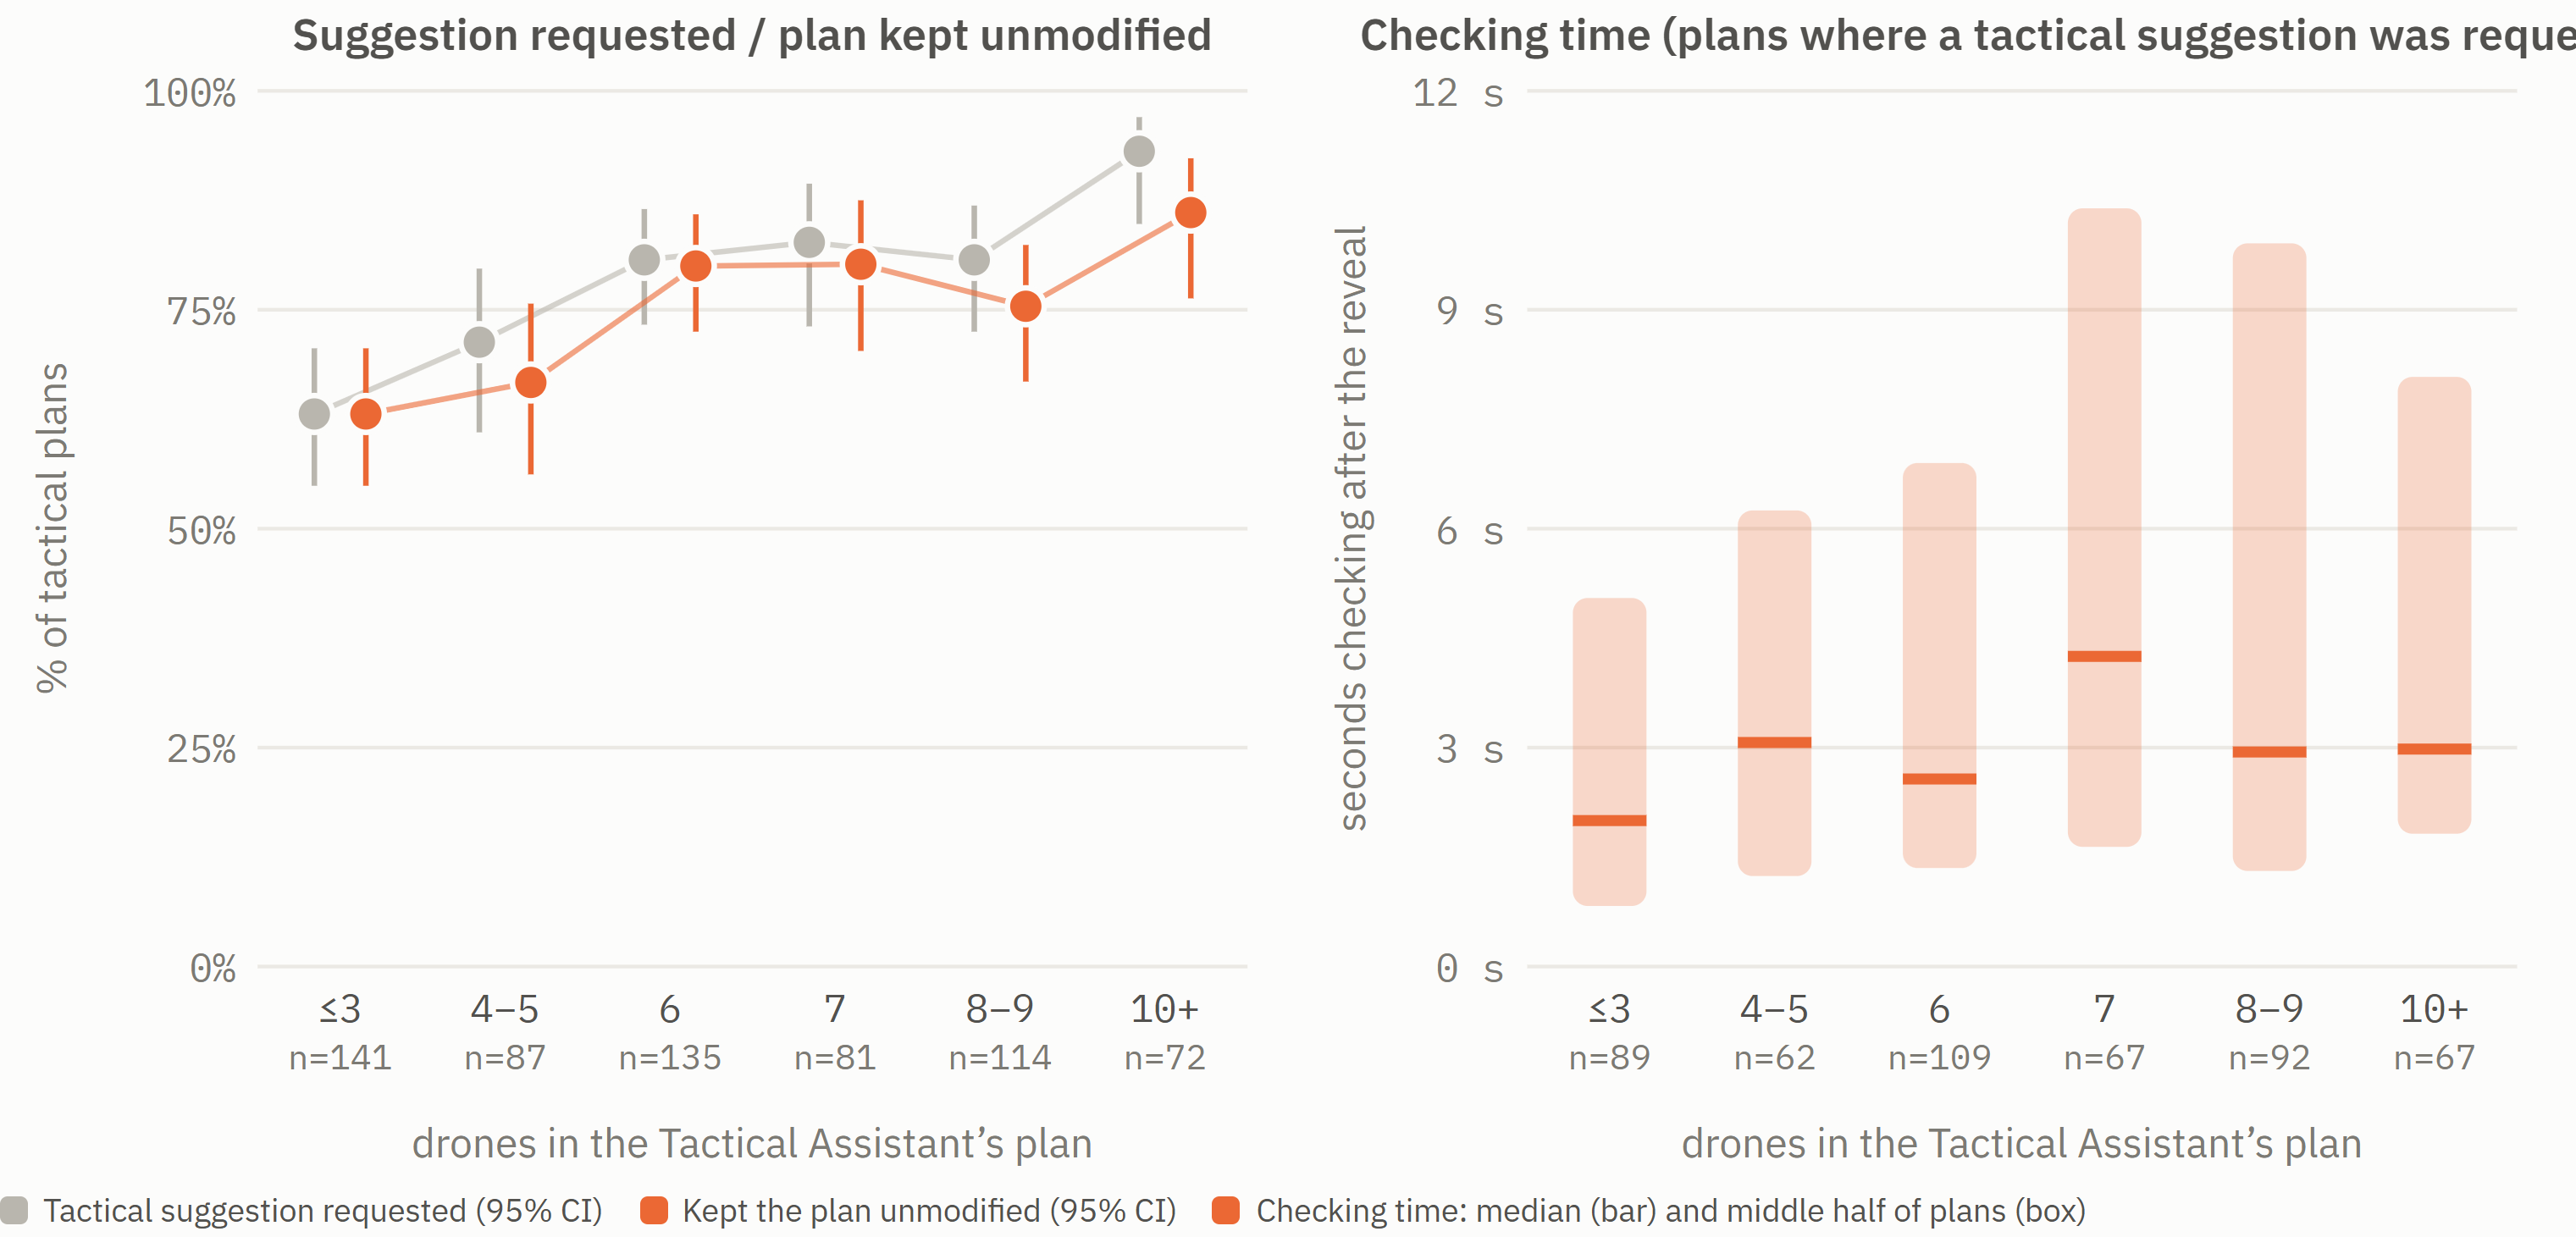
\includegraphics[width=\linewidth,height=0.50\textheight,keepaspectratio]{figs/results/f-tier-trust__checking__main.png}
\caption{\textbf{Checking a tactical plan takes a few seconds, whatever its size.} By plan size: the share of plans with a suggestion requested, the share kept unmodified, and the median checking time once Deploy unlocks.}
\label{fig:res:tier-trust:checking}
\end{figure}

Trust and use line up when people are ranked against each other (the trust gap correlates $\rho = .47$ with the gap in use), but not in size and not over time: a change in a person's trust from one session to the next does not go with a change in their use ($\rho = .16$), and trust after the first session does not predict how their use changes in the second ($\rho = .07$).

\begin{options}
\optshead{Options for this finding}

\optsec{Trusted more: the basic result} {\footnotesize [pass 5: for the paper]}

\noindent Key numbers:\begin{itemize}[leftmargin=1.2em,itemsep=0pt]\footnotesize
\item Strategic 4.61 [4.18, 5.04], Tactical 5.44 [5.15, 5.73] (1--7, person means)
\item Gap +0.83 [+0.35, +1.30]; paired t p = .0012; Wilcoxon p = .0010; dz = .62; n = 33
\item 26 higher for tactical, 6 for strategic, 1 tied
\item Item gaps: follow its recommendations +1.11, I trust it +1.01, reliable +0.94, performs well +0.74, useful +0.67 (all p < .01); confident in it +0.48 (p = .13)
\end{itemize}

\noindent Highlighted quotes not used above:\begin{quotelist}
\item ``But I think in the [tactical level], it works very well.''\,---\,P33 (debrief 0:28:24)
\end{quotelist}

\optsec{Where the gap comes from: the second session and the Strategic Heavy scenario} {\footnotesize [pass 5: for the paper]}

\par\noindent \begin{minipage}[t]{0.49\linewidth}\centering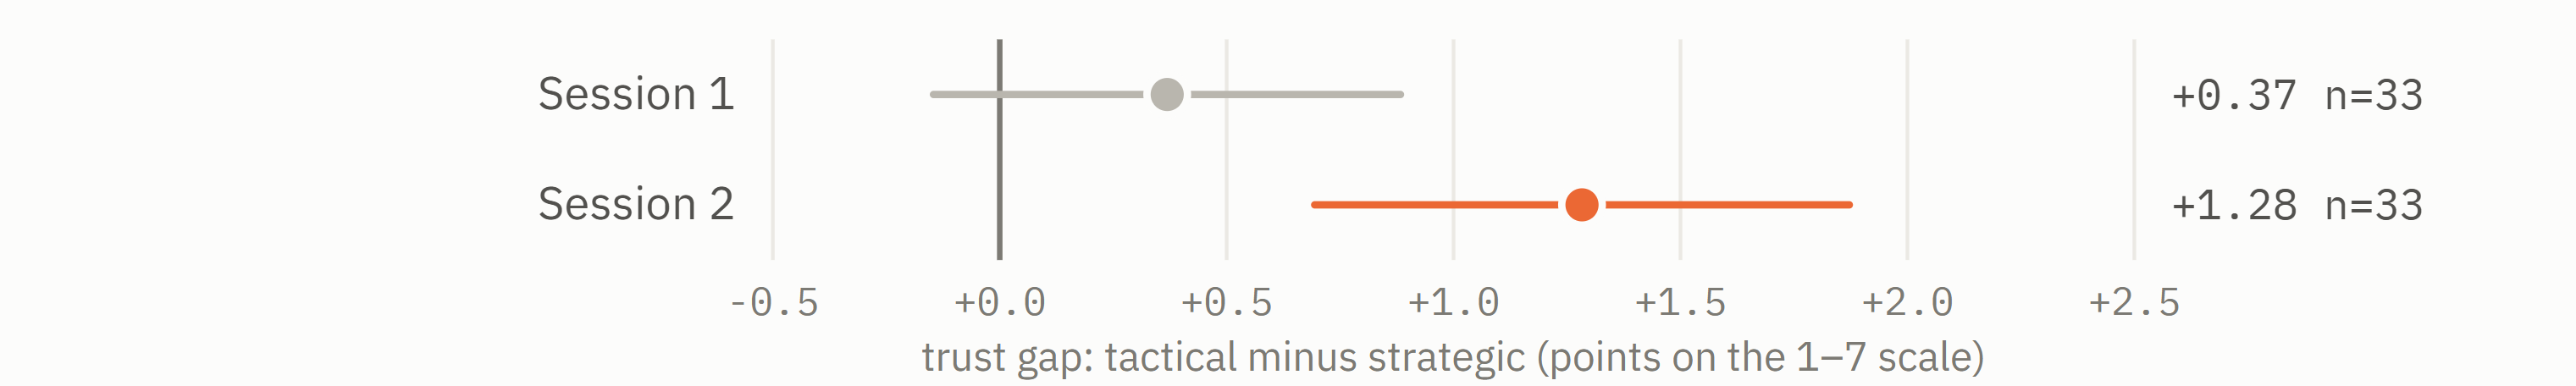
\includegraphics[width=\linewidth,height=0.24\textheight,keepaspectratio]{figs/results/f-tier-trust__where__session.png}\par{\scriptsize Other view: By session order as well.}\end{minipage}

\noindent Key numbers:\begin{itemize}[leftmargin=1.2em,itemsep=0pt]\footnotesize
\item Session 1 gap +0.37 [$-$0.15, +0.88]; session 2 +1.28 [+0.69, +1.87] (n = 33 each)
\item Strategic Heavy sessions +1.13 [+0.53, +1.73]; Tactical Heavy sessions +0.52 [$-$0.01, +1.05] (n = 33 each)
\item Same people, Strategic Heavy minus Tactical Heavy: +0.61 [$-$0.01, +1.23], paired t p = .054, Wilcoxon p = .038; strategic trust $-$0.46 (p = .087), tactical +0.15 (p = .25)
\item Both in one model: Strategic Heavy +0.64 [+0.11, +1.17], p = .019; second session +0.93 [+0.40, +1.47], p < .001
\item Strategic trust 5.00 $\rightarrow$ 4.23 from session 1 to 2; tactical 5.36 $\rightarrow$ 5.51
\end{itemize}

\optsec{Why the tactical plan is kept: checking it is brief and does not grow with the plan} {\footnotesize [pass 5: for the paper]}

\noindent Key numbers:\begin{itemize}[leftmargin=1.2em,itemsep=0pt]\footnotesize
\item Kept unmodified rises with plan size: OR 1.76 per SD [1.25, 2.47], p = .001 (all 630 plans)
\item Consulted rises: OR 2.52 [1.87, 3.38]; kept once consulted FALLS: OR 0.68 [0.50, 0.94], p = .017
\item By bin ($\leq$3, 4--5, 6, 7, 8--9, 10+ drones; n = 141, 87, 135, 81, 114, 72 plans): suggestion requested 63\%, 71\%, 81\%, 83\%, 81\%, 93\%; kept unmodified 63\%, 67\%, 80\%, 80\%, 75\%, 86\%
\item 10+ drones vs $\leq$3: suggestion requested 93\% vs 63\%, OR 10.8 [3.2, 36.0]; kept 86\% vs 63\%, OR 5.2 [2.1, 12.7], both p < .001
\item Median checking time by bin: 2.0, 3.1, 2.6, 4.2, 2.9, 3.0 s; per SD +0.60 s [$-$0.15, +1.35], p = .12; per drone 0.68 s at $\leq$3 drones $\rightarrow$ 0.23 s at 10+
\item 468 of 486 consulted plans deployed unmodified (96\%)
\item Person-median check: tactical 2.85 s vs strategy card 8.80 s (n = 33, Wilcoxon p < .0001)
\item H2 primary p = .019 uncorrected, .065 after Holm correction across round 1
\end{itemize}

\noindent Highlighted quotes not used above:\begin{quotelist}
\item ``My reason is there are so many drones, so I don't have enough energy and attention to just the check them.''\,---\,P27 (think-aloud s1 0:56)
\end{quotelist}

\optsec{Stated vs revealed preference: they line up in rank, not in size or over time} {\footnotesize [pass 5: numbers only]}

\par\noindent \begin{minipage}[t]{0.49\linewidth}\centering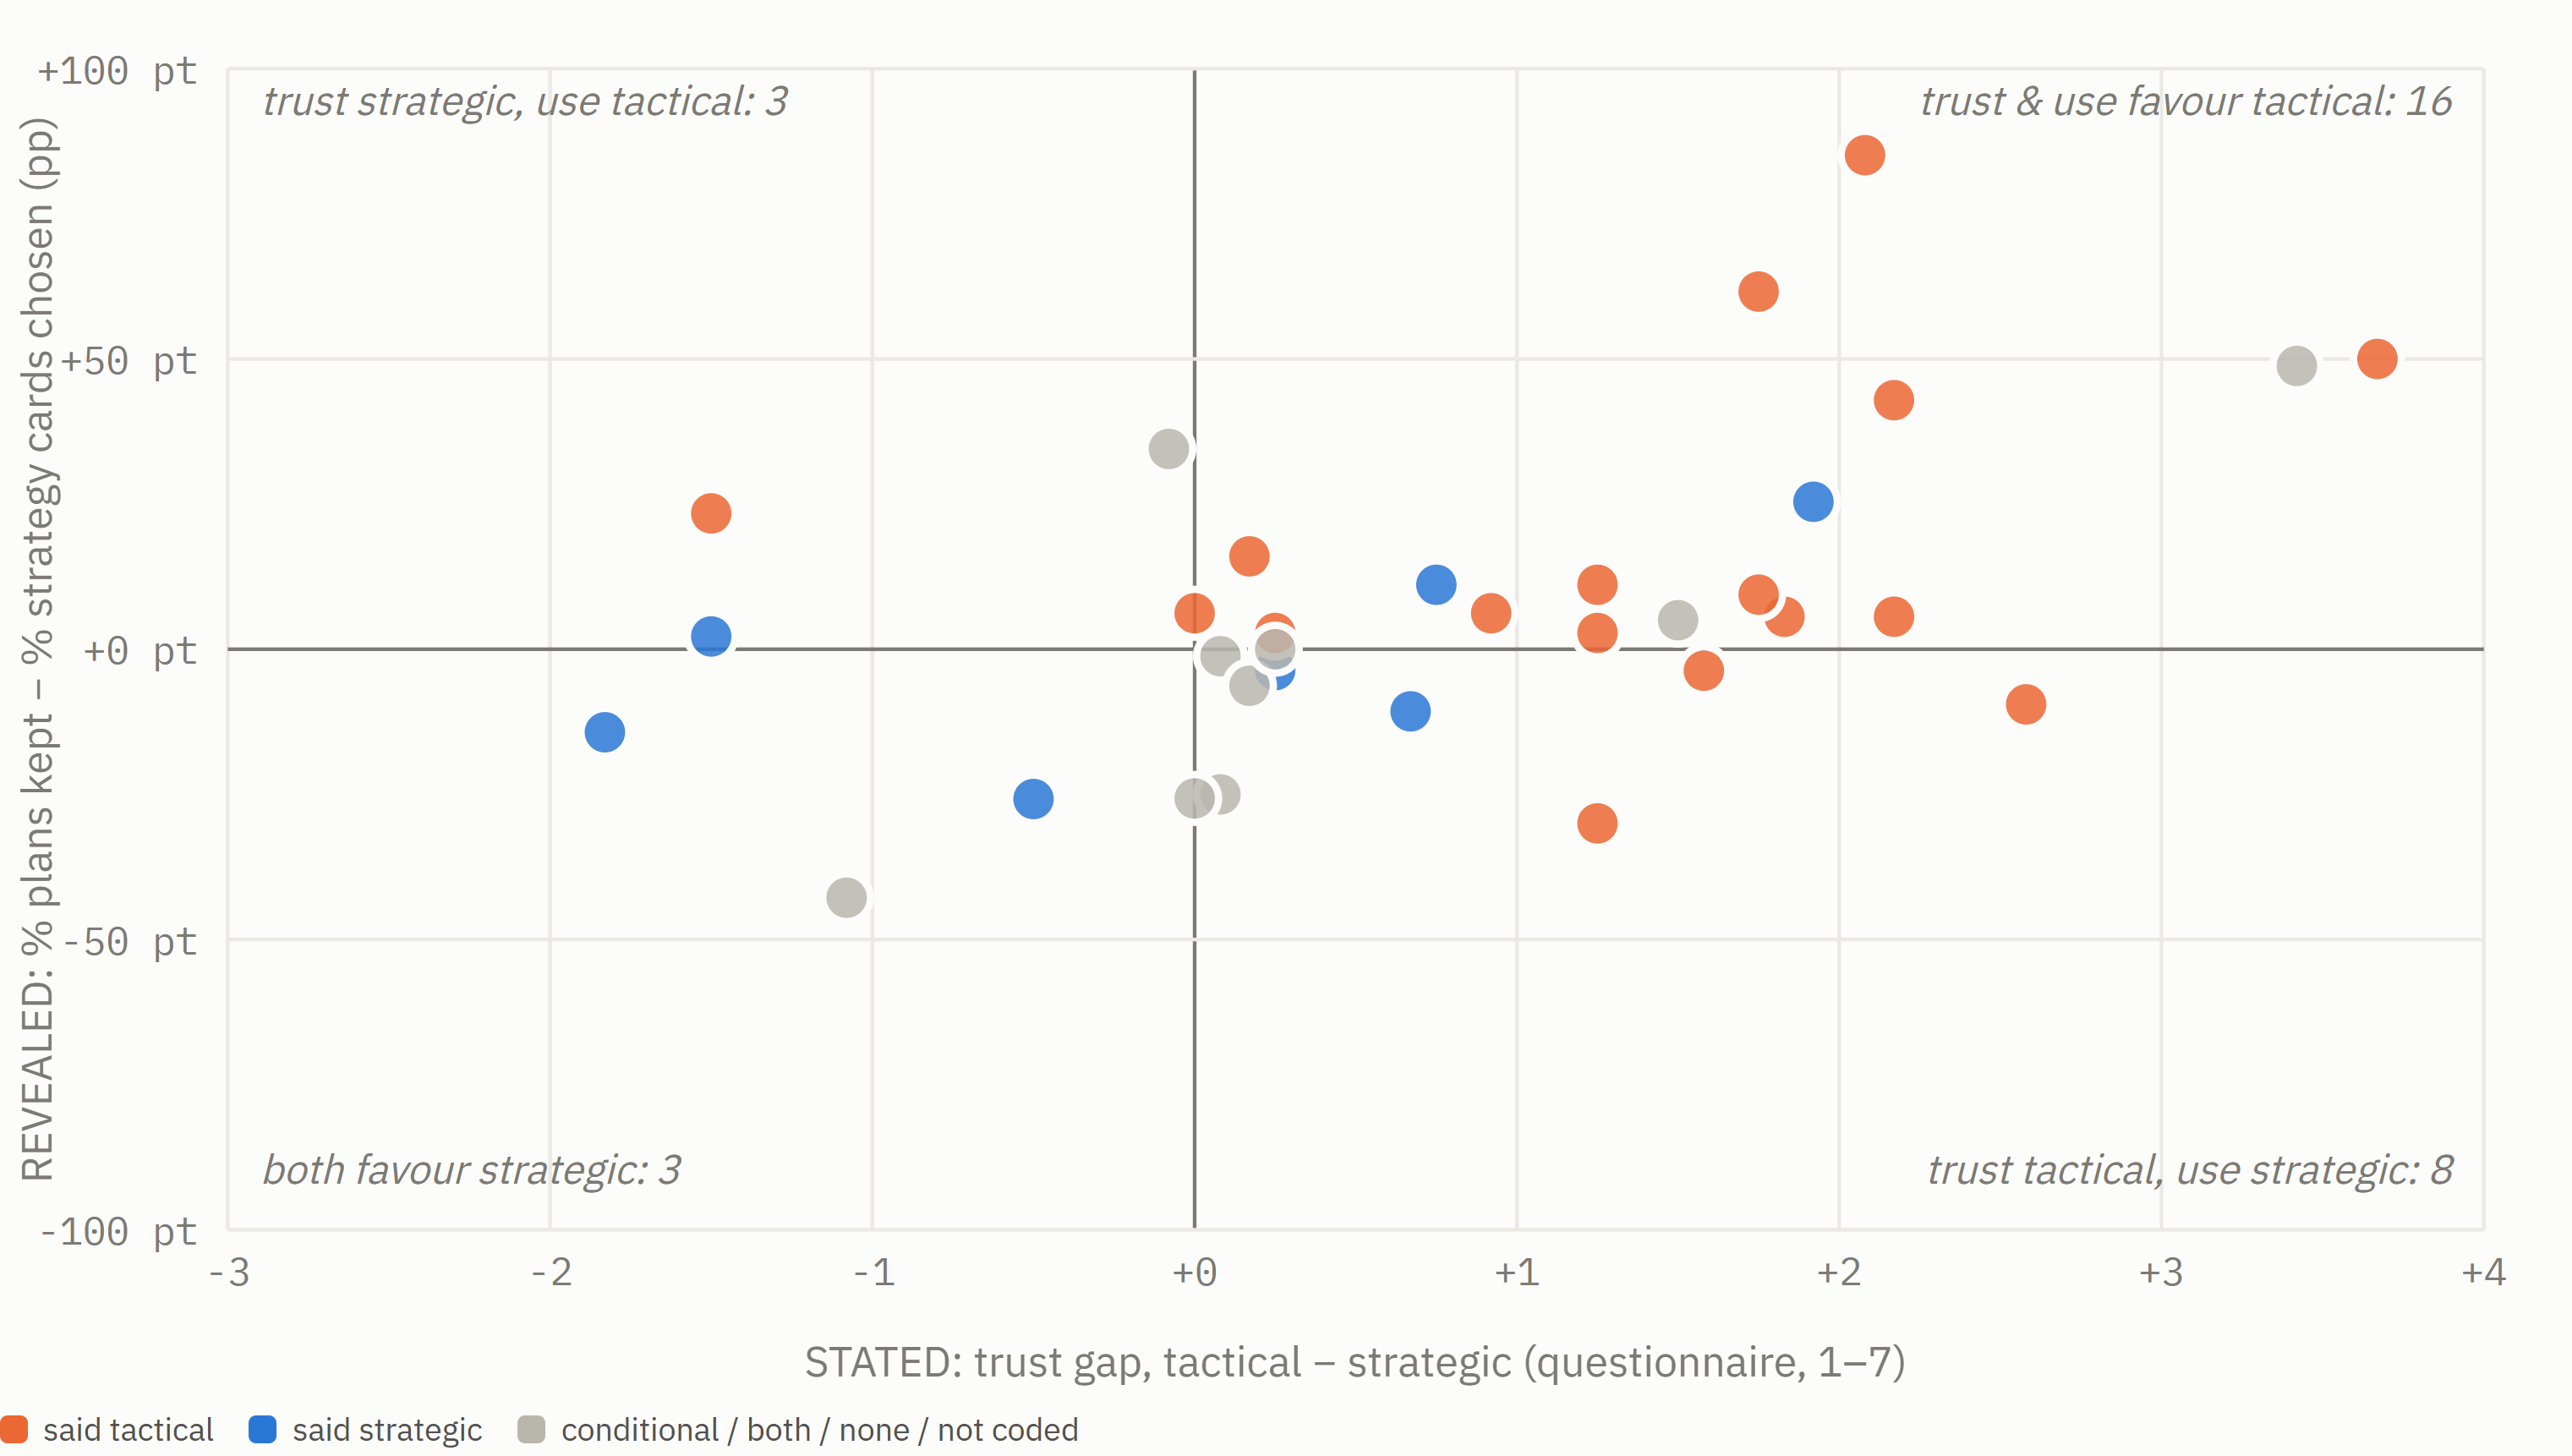
\includegraphics[width=\linewidth,height=0.24\textheight,keepaspectratio]{figs/results/f-tier-trust__stated-revealed__kept.png}\par{\scriptsize Other view: Use measured as keeping the plan unmodified.}\end{minipage}\hfill
\begin{minipage}[t]{0.49\linewidth}\centering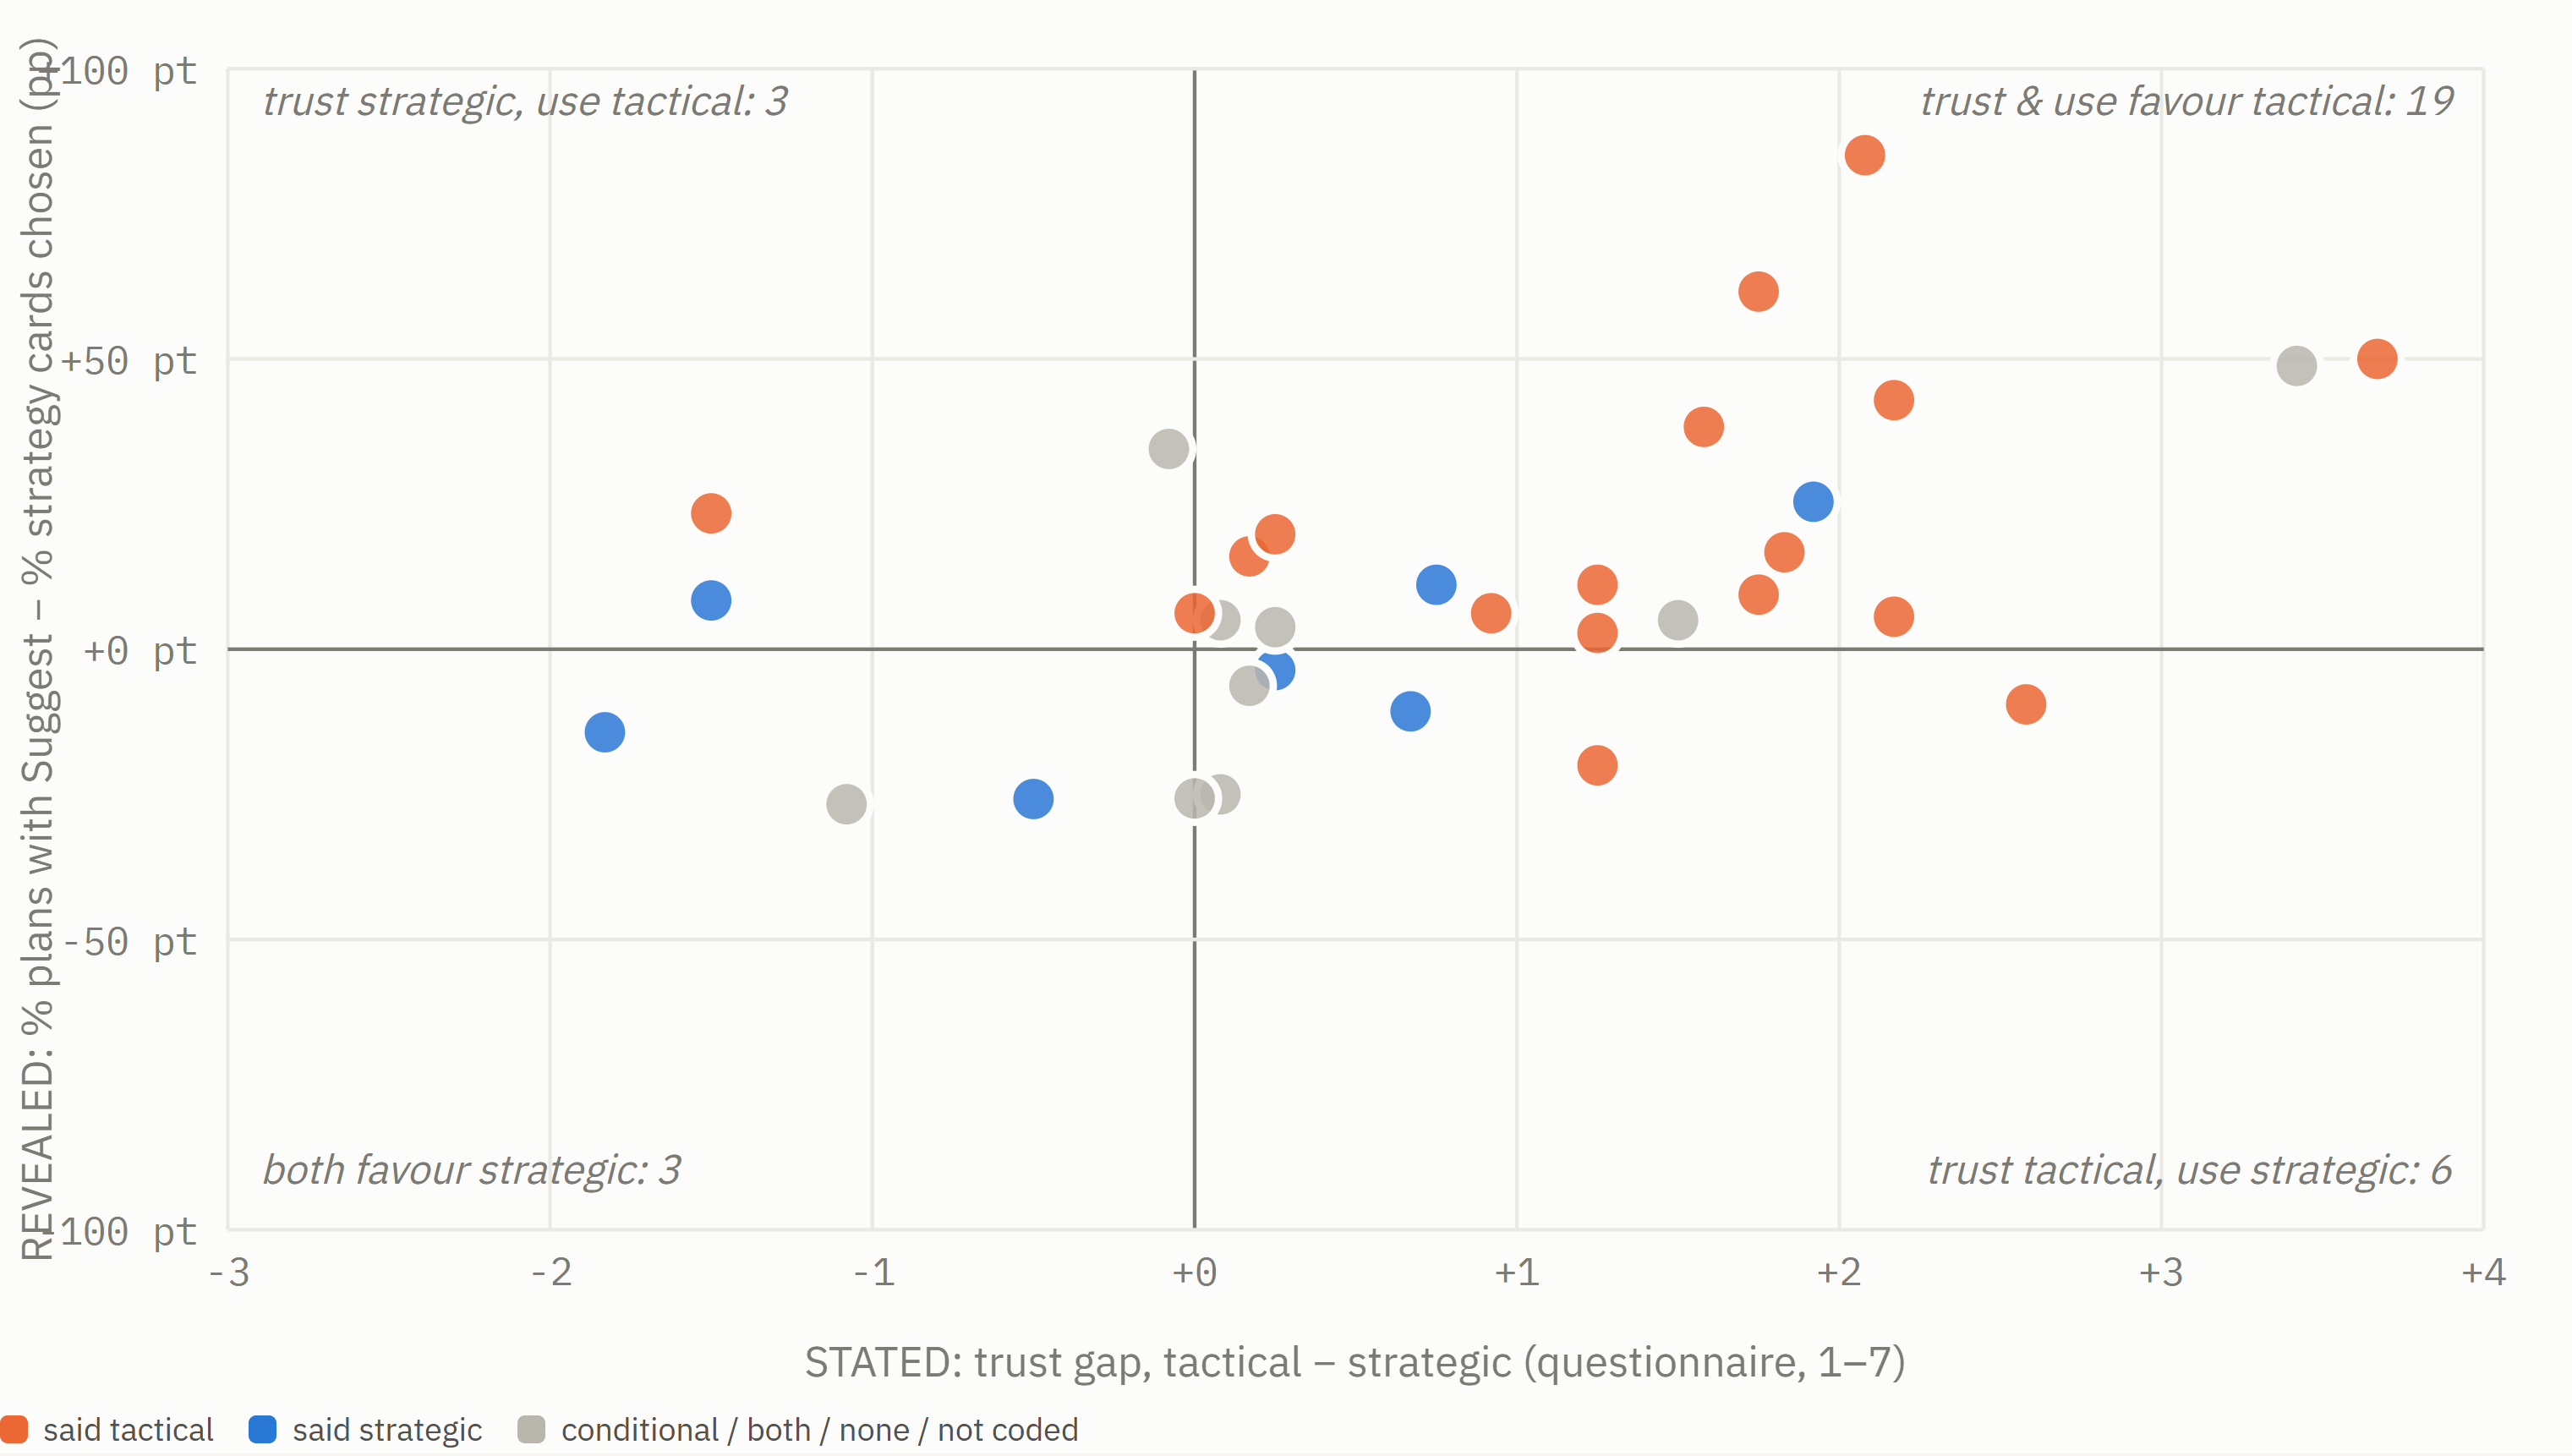
\includegraphics[width=\linewidth,height=0.24\textheight,keepaspectratio]{figs/results/f-tier-trust__stated-revealed__pressed.png}\par{\scriptsize Other view: Use measured as pressing Suggest at all.}\end{minipage}

\noindent Key numbers:\begin{itemize}[leftmargin=1.2em,itemsep=0pt]\footnotesize
\item Trust gap vs usage gap (kept $-$ took): $\rho$ = .47 [.10, .73], p = .006, n = 33
\item Quadrants: both favour tactical 16, both strategic 3, trust tactical/use strategic 9, trust strategic/use tactical 3 (2 on a zero line)
\item Group use: chose a strategy card 64\%, consulted the plan 76\%, kept it 72\%; usage gap +0.08 [$-$0.02, +0.17]
\item Within person, change in strategic trust vs change in strategy card use: $\rho$ = .16 [$-$.27, .52], p = .38
\item Session-1 strategic trust vs change in strategy card use s1$\rightarrow$s2: $\rho$ = .07 [$-$.27, .40], p = .71; tactical .01
\item Between people, strategic trust vs strategy cards chosen $\rho$ = .60 [.30, .78]; tactical trust vs plan kept $\rho$ = .31, p = .08
\end{itemize}

\optsec{All the trust--use correlations in one view} {\footnotesize [pass 5: numbers only]}

\par\noindent \begin{minipage}[t]{0.49\linewidth}\centering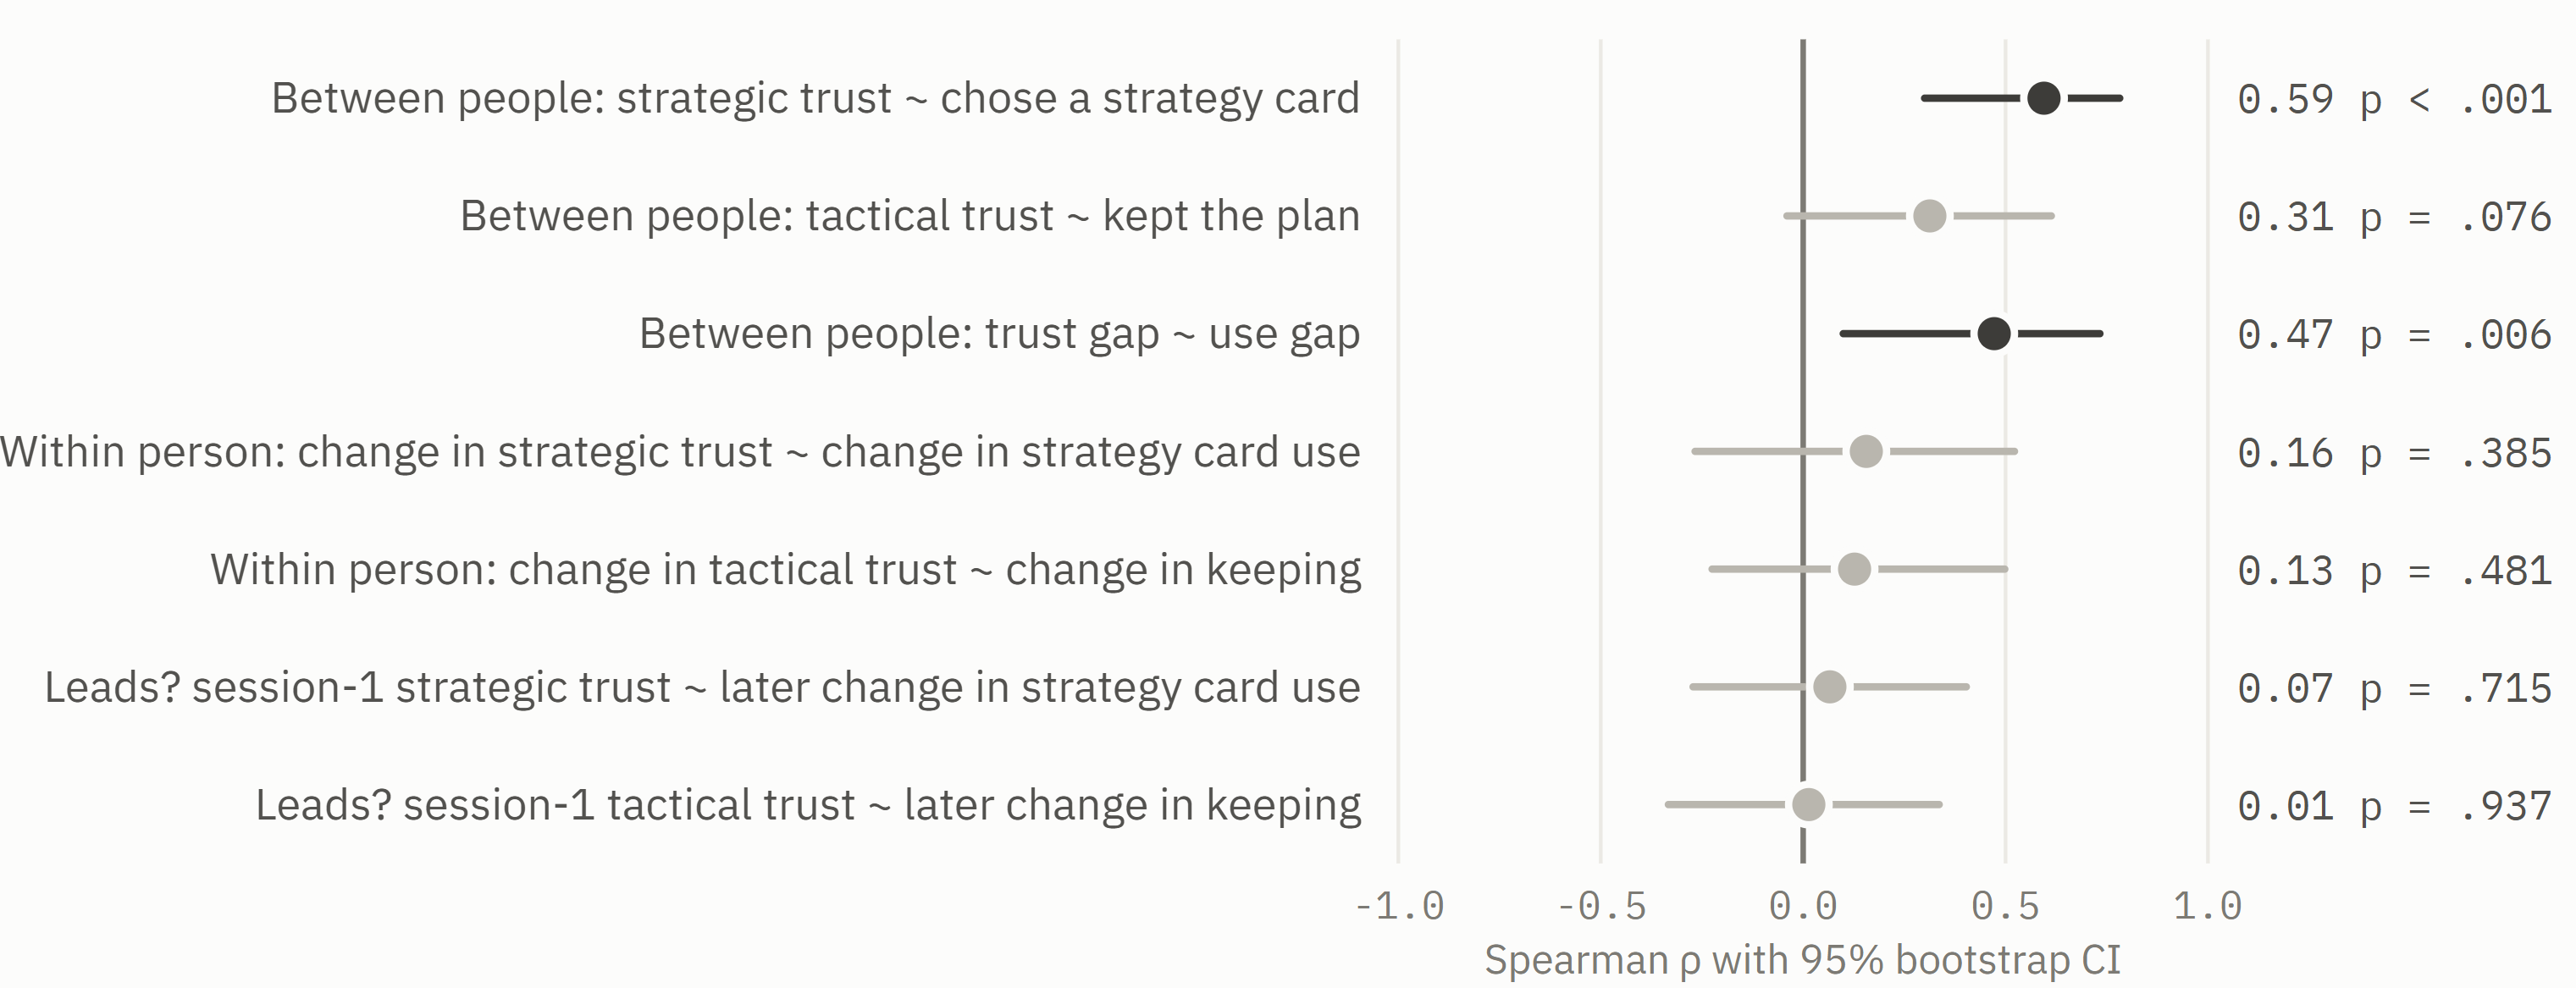
\includegraphics[width=\linewidth,height=0.24\textheight,keepaspectratio]{figs/results/f-tier-trust__trust-lead-strip__main.png}\par{\scriptsize Other view: main}\end{minipage}
\end{options}

\clearpage

% ======== f-operator-wants ========

\subsection{What operators asked for}\label{sec:res:operator-wants}

Asked about real search and rescue, nobody rejected assistants like these, and 9 of 33 said, mostly unprompted, that a human must keep the final decision. What they asked for was mostly information: how the assistants decide, and how likely drones were to fail.

% --- f-operator-wants#wants (pass 5: numbers only) ---

\phantomsection\label{sec:res:operator-wants:wants}\label{sec:res:operator-wants:real-world}\label{sec:res:operator-wants:reasoning}\label{sec:res:operator-wants:failure-data}\label{sec:res:operator-wants:more-automation}\label{sec:res:operator-wants:mental-models}\label{sec:res:operator-wants:tiers-together}\label{sec:res:operator-wants:me-vs-assistant}\label{sec:res:operator-wants:interface}\label{sec:res:operator-wants:real-stakes}\label{sec:res:operator-wants:feelings}
Figure~\ref{fig:res:operator-wants:wants} counts the requests. Beyond a human final say, the most common were failure probabilities or performance data (6), options between the two strategy cards (6) and the assistants' reasoning (5); only four wanted the assistants to do more. Several credited the assistants with more than they had, assuming they learned from the operator or that the two tiers shared one plan, while others saw through them to simple rules. These themes are taken up in Section~\ref{sec:qual}.

\begin{figure}[H]
\centering
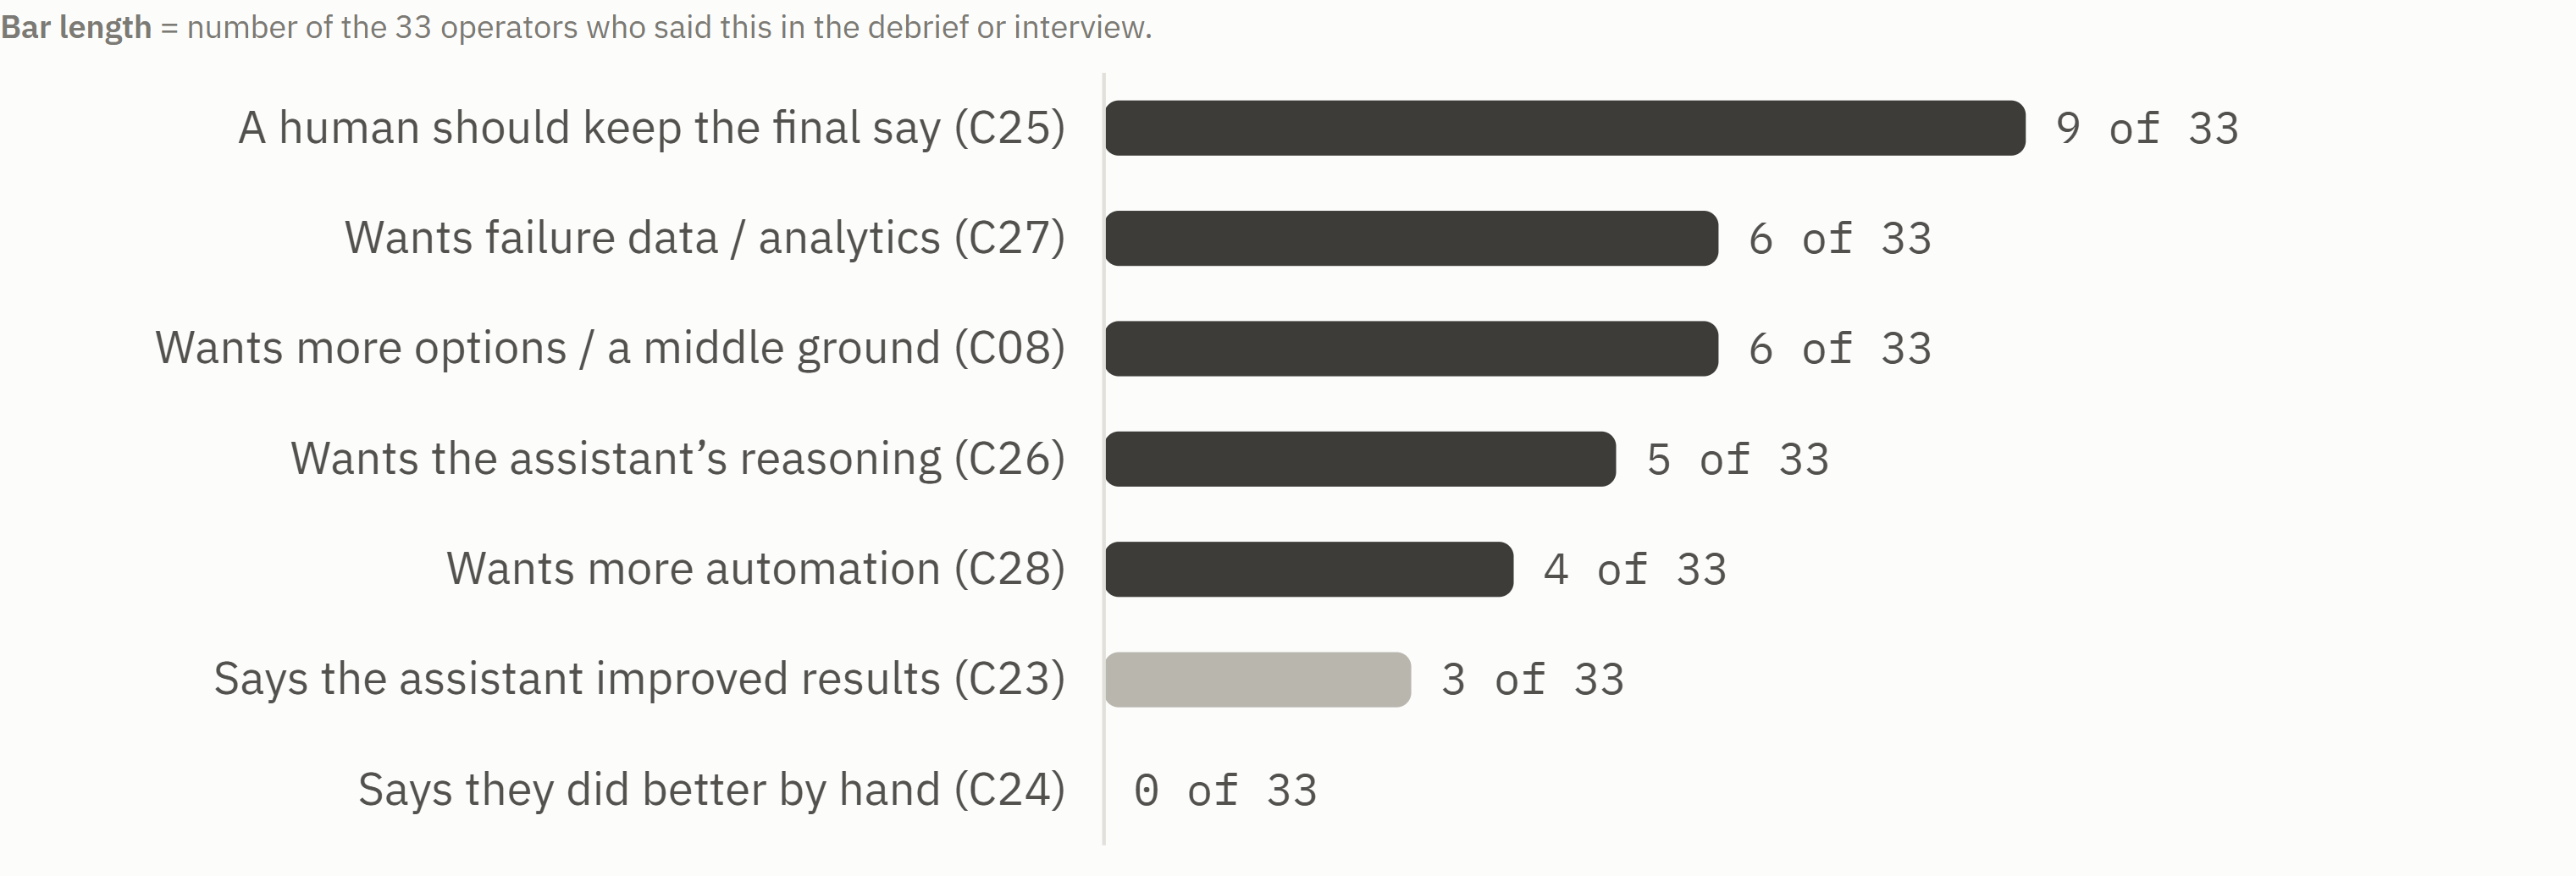
\includegraphics[width=\linewidth,height=0.50\textheight,keepaspectratio]{figs/results/f-operator-wants__wants__main.png}
\caption{\textbf{What operators asked for.} Number of participants raising each request (of 33).}
\label{fig:res:operator-wants:wants}
\end{figure}

\begin{options}
\optshead{Options for this finding}

\optsec{What they asked for} {\footnotesize [pass 5: numbers only]}

\noindent Key numbers:\begin{itemize}[leftmargin=1.2em,itemsep=0pt]\footnotesize
\item Human final say 9 of 33 (8 unprompted); failure data 6; more options 6; reasoning 5; more automation 4 (all unprompted)
\end{itemize}
\end{options}

\clearpage
